\documentclass[10pt,a4paper]{article}
\usepackage[margin=1.7cm]{geometry}
\usepackage{amsmath}
\usepackage{tikz}
\usetikzlibrary{arrows.meta,positioning,shapes.geometric,fit,calc}
\usepackage[most]{tcolorbox}
\usepackage{booktabs,tabularx}
\usepackage{enumitem}
\usepackage{titlesec}
\usepackage{xcolor}
\usepackage{colortbl}
\usepackage[hidelinks]{hyperref}
\setlist{nosep,leftmargin=1.2em}
\setlength{\parindent}{0pt}
\setlength{\parskip}{3pt}
\setlength{\emergencystretch}{3em}
\titlespacing*{\section}{0pt}{8pt}{4pt}
\titlespacing*{\subsection}{0pt}{6pt}{2pt}

% ---------- Atom One Light theme ----------
\makeatletter
\def\XC@clr@rgb@white{0.98039,0.98039,0.98039}% #FAFAFA
\def\XC@clr@gray@white{0.98}
\makeatother
\definecolor{white}{HTML}{FAFAFA}   % background
\definecolor{black}{HTML}{383A42}   % foreground
\definecolor{red}{HTML}{E45649}
\definecolor{orange}{HTML}{986801}
\definecolor{yellow}{HTML}{C18401}
\definecolor{green}{HTML}{50A14F}
\definecolor{cyan}{HTML}{0184BC}
\definecolor{blue}{HTML}{4078F2}
\definecolor{magenta}{HTML}{A626A4}
\definecolor{brown}{HTML}{986801}
\definecolor{gray}{HTML}{A0A1A7}
\definecolor{acc}{HTML}{4078F2}     % blue: headings, key boxes
\definecolor{warn}{HTML}{E45649}    % red: exam tips, highlights
\definecolor{ok}{HTML}{50A14F}      % green
\pagecolor{white}
\AtBeginDocument{\color{black}\def\normalcolor{\color{black}}}
\tcbset{colupper=black,collower=black,coltitle=white}% tcolorbox froze the old black/white at load time
% code font
\usepackage{fontspec}
% text: Fira Sans (pairs with Fira Math); code: AnnotationM
\setmainfont{FiraSans}[Extension=.otf,UprightFont=*-Regular,BoldFont=*-SemiBold,ItalicFont=*-Italic,BoldItalicFont=*-SemiBoldItalic]
\setsansfont{FiraSans}[Extension=.otf,UprightFont=*-Regular,BoldFont=*-SemiBold,ItalicFont=*-Italic,BoldItalicFont=*-SemiBoldItalic]
\setmonofont{AnnotationM Nerd Font Mono}[Scale=MatchLowercase]
\usepackage{unicode-math}
\setmathfont{FiraMath-Regular.otf}[Scale=0.95]
% glyphs missing from AnnotationM and Fira Math: take them from STIX Two
\newfontfamily\symfallback{STIXTwoMath-Regular.otf}
\AtBeginDocument{\renewcommand{\checkmark}{\text{\symfallback\char"2713}}\renewcommand{\bigstar}{\text{\symfallback\char"2605}}}
\titleformat{\section}{\large\bfseries\color{acc}}{\thesection}{0.6em}{}
\titleformat{\subsection}{\normalsize\bfseries}{\thesubsection}{0.5em}{}

\newtcolorbox{keybox}[1][]{colback=acc!6,colframe=acc,boxrule=0.6pt,arc=2pt,left=4pt,right=4pt,top=2pt,bottom=2pt,fonttitle=\bfseries\small,#1}
\newtcolorbox{examtip}{colback=warn!6,colframe=warn,boxrule=0.6pt,arc=2pt,left=4pt,right=4pt,top=2pt,bottom=2pt,title=Exam tips,fonttitle=\bfseries\small}
\newtcolorbox{trap}[1][]{colback=warn!6,colframe=warn,boxrule=0.6pt,arc=2pt,left=4pt,right=4pt,top=2pt,bottom=2pt,title={Trap#1},fonttitle=\bfseries\small}
\newtcolorbox{fixbox}{colback=gray!6,colframe=gray!60,boxrule=0.6pt,arc=2pt,left=4pt,right=4pt,top=2pt,bottom=2pt,title=Corrections to the notes / slides,fonttitle=\bfseries\small,coltitle=black}

\tikzset{
  box/.style={draw,rounded corners=2pt,align=center,font=\small,minimum height=7mm,inner sep=3pt},
  circ/.style={draw,circle,fill=orange!25,font=\small\bfseries,minimum size=8mm},
  arr/.style={-{Stealth[length=2mm]},thick},
  darr/.style={{Stealth[length=2mm]}-{Stealth[length=2mm]},thick}
}
\newcommand{\hl}[1]{\cellcolor{warn!18}\textbf{#1}}
\newcommand{\ttx}[1]{\texttt{#1}}

\usepackage[normalem]{ulem}
\newcommand{\pfcell}[3]{\fill[#3] (#1-1,1-#2) rectangle (#1,-#2);}
\newcommand{\pfletters}[1]{%
  \foreach \row [count=\r] in #1{\foreach \l [count=\c] in \row {\node[font=\small] at (\c-0.5,0.5-\r) {\l};}}
  \foreach \i in {0,...,5}{\draw[gray!70] (\i,0) -- (\i,-5); \draw[gray!70] (0,-\i) -- (5,-\i);}}
\newcommand{\MONARCHY}{{M,O,N,A,R},{C,H,Y,B,D},{E,F,G,{I/J},K},{L,P,Q,S,T},{U,V,W,X,Z}}
\setcounter{tocdepth}{1}

\begin{document}

\begin{center}
{\LARGE\bfseries Cryptography \& Network Security}\\[2pt]
{\large Study Notes}
\end{center}
{\small\tableofcontents}

% Videos: network security model, symmetric cipher model, types of crypto, security of schemes
\section{Model for Network Security}

Sender $S$ wants to send a message to receiver $R$ over an insecure channel (the Internet). An \textbf{opponent} can sniff the channel.

\begin{center}
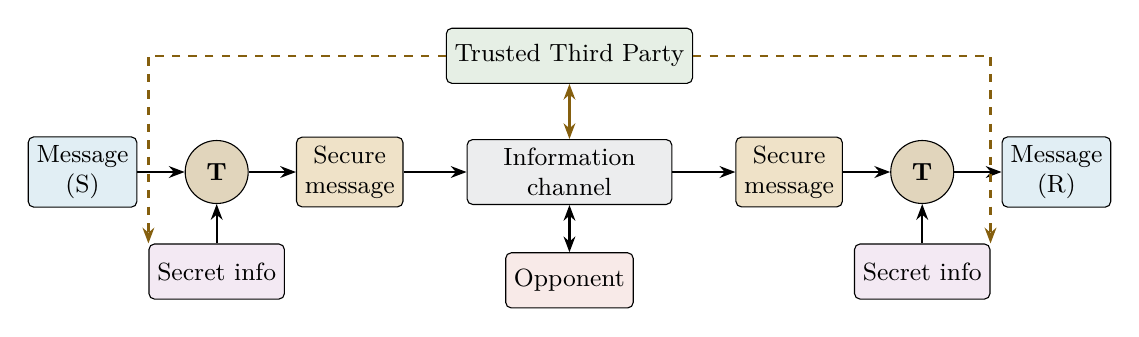
\begin{tikzpicture}[node distance=6mm]
  \node[box,fill=cyan!10] (m1) {Message\\(S)};
  \node[circ,right=of m1] (t1) {T};
  \node[box,below=5mm of t1,fill=magenta!8] (k1) {Secret info};
  \node[box,right=of t1,fill=yellow!20] (c1) {Secure\\message};
  \node[box,right=8mm of c1,minimum width=26mm,fill=gray!15] (ch) {Information\\channel};
  \node[box,right=8mm of ch,fill=yellow!20] (c2) {Secure\\message};
  \node[circ,right=of c2] (t2) {T};
  \node[box,below=5mm of t2,fill=magenta!8] (k2) {Secret info};
  \node[box,right=of t2,fill=cyan!10] (m2) {Message\\(R)};
  \node[box,below=6mm of ch,fill=red!10] (op) {Opponent};
  \node[box,above=7mm of ch,fill=green!12] (ttp) {Trusted Third Party};
  \draw[arr] (m1)--(t1); \draw[arr] (k1)--(t1); \draw[arr] (t1)--(c1);
  \draw[arr] (c1)--(ch); \draw[arr] (ch)--(c2);
  \draw[arr] (c2)--(t2); \draw[arr] (k2)--(t2); \draw[arr] (t2)--(m2);
  \draw[darr] (op)--(ch);
  \draw[darr,orange!80!black] (ttp)--(ch);
  \draw[arr,orange!80!black,dashed] (ttp.west) -| (k1.north west);
  \draw[arr,orange!80!black,dashed] (ttp.east) -| (k2.north east);
\end{tikzpicture}
\end{center}

\begin{itemize}
  \item \textbf{T (security-related transformation)} takes two inputs: the message and \textbf{secret info} (a key). Output: a secure message (ciphertext). $R$ applies the reverse $T$ with its secret info.
  \item It is called $T$, not $E$, because encryption is only one option. \textbf{Steganography} (hiding data inside an image, audio, etc.) is another.
  \item The opponent can intercept the secure message but cannot read it.
  \item Security rests on the \textbf{key} (its secrecy and bit length) and algorithm strength, not on hiding the algorithm. Small key space $\Rightarrow$ brute force works.
  \item \textbf{Trusted Third Party (TTP)}: distributes keys, issues certificates, settles disputes. Example: a Certificate Authority signing a bank's SSL certificate. (Details come later in the course.)
\end{itemize}

\subsection{Four tasks in designing a security service}
\begin{keybox}
\begin{enumerate}[leftmargin=1.5em]
  \item \textbf{Design an algorithm} for $T$ (encrypt at $S$, decrypt at $R$) that the opponent cannot defeat.
  \item \textbf{Generate the secret information} (large keys, so brute force is infeasible).
  \item \textbf{Develop methods to distribute and share} the secret info (get keys to $S$ and $R$ safely).
  \item \textbf{Specify a protocol}: the rules both parties follow to use the algorithm and keys (e.g., SSL/TLS, IPsec).
\end{enumerate}
\end{keybox}
Memory aid: \emph{Algorithm $\to$ Key $\to$ Distribute $\to$ Protocol}.

\section{Network Access Security Model}

Protects a \emph{system} from unwanted access, rather than protecting a message in transit.

\begin{center}
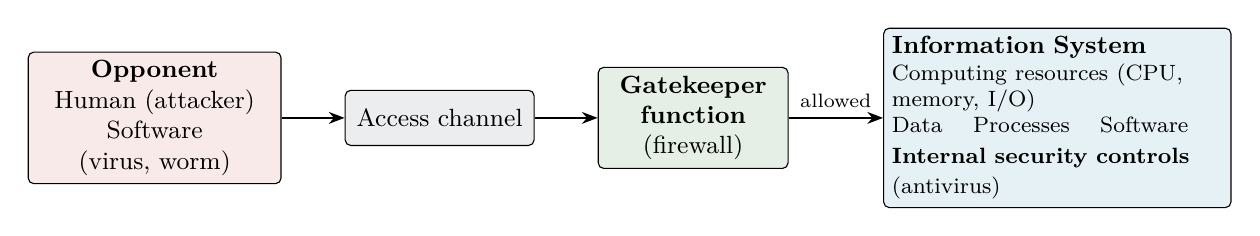
\begin{tikzpicture}[node distance=8mm]
  \node[box,fill=red!10,text width=30mm] (op) {\textbf{Opponent}\\Human (attacker)\\Software (virus, worm)};
  \node[box,right=of op,fill=gray!15,minimum width=24mm] (ac) {Access channel};
  \node[box,right=of ac,fill=green!12,text width=22mm] (gk) {\textbf{Gatekeeper function}\\(firewall)};
  \node[box,right=12mm of gk,fill=cyan!8,text width=42mm,align=left] (is) {\textbf{Information System}\\
    \footnotesize Computing resources (CPU, memory, I/O)\\ \footnotesize Data \quad Processes \quad Software\\
    \footnotesize\textbf{Internal security controls} (antivirus)};
  \draw[arr] (op)--(ac); \draw[arr] (ac)--(gk); \draw[arr] (gk)--node[above,font=\scriptsize]{allowed} (is);
\end{tikzpicture}
\end{center}

\begin{itemize}
  \item \textbf{Opponent}: a human hacker or malicious software.
  \item \textbf{Gatekeeper}: first line of defence, like a guard at a gate. Filters traffic and blocks intruders (firewall, login checks).
  \item \textbf{Internal security controls}: second line, inside the system, catching what slips past the gate (antivirus, OS permissions).
  \item Insiders (e.g., employees) can also attack, but this model focuses on outside threats.
\end{itemize}

\section{Cryptography}

\begin{keybox}[title=Definition]
The art or science of transforming an \textbf{intelligible} message (plaintext) into an \textbf{unintelligible} one (ciphertext), and then \textbf{retransforming} it back to the original form.
\end{keybox}

\subsection{Symmetric cipher model}
\begin{center}
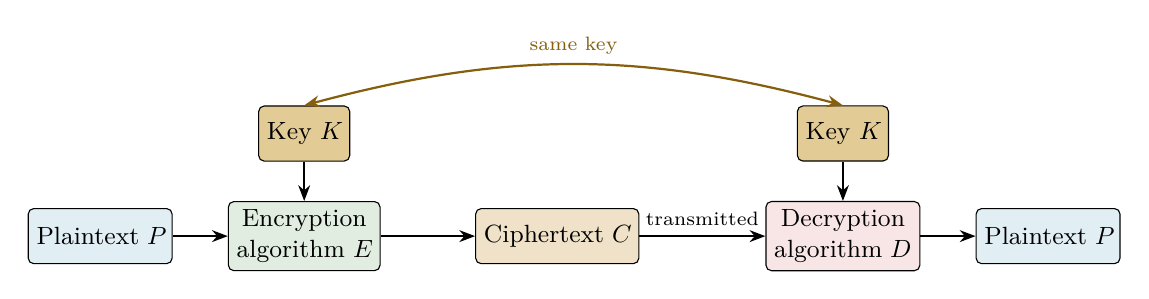
\begin{tikzpicture}[node distance=7mm]
  \node[box,fill=cyan!10] (p1) {Plaintext $P$};
  \node[box,right=of p1,fill=green!15] (e) {Encryption\\algorithm $E$};
  \node[box,right=12mm of e,fill=yellow!20] (c) {Ciphertext $C$};
  \node[box,right=16mm of c,fill=red!12] (d) {Decryption\\algorithm $D$};
  \node[box,right=of d,fill=cyan!10] (p2) {Plaintext $P$};
  \node[box,above=5mm of e,fill=yellow!40] (k1) {Key $K$};
  \node[box,above=5mm of d,fill=yellow!40] (k2) {Key $K$};
  \draw[arr] (p1)--(e); \draw[arr] (k1)--(e); \draw[arr] (e)--(c);
  \draw[arr] (c)--node[above,font=\scriptsize]{transmitted}(d); \draw[arr] (k2)--(d); \draw[arr] (d)--(p2);
  \draw[darr,bend left=15,orange!80!black] (k1.north) to node[above,font=\scriptsize]{same key} (k2.north);
\end{tikzpicture}
\end{center}
\[
C = E(K, P) \qquad\qquad P = D(K, C) = D\big(K, E(K,P)\big)
\]
\begin{itemize}
  \item Encryption needs \textbf{two} inputs ($P$ and $K$); decryption needs $C$ and $K$.
  \item $E$ and $D$ are \textbf{public}. Only $K$ is secret (Kerckhoffs's principle).
  \item If $K$ leaks, \emph{all} past and future messages between $S$ and $R$ can be read.
  \item Toy example: $K = 100$ at both ends. Real keys are huge (128, 256, 2048 bits), so guessing is infeasible.
\end{itemize}

\subsection{Types of cryptography}
\begin{center}
\small
\begin{tabularx}{\textwidth}{@{}l X X@{}}
\toprule
 & \textbf{Symmetric} (private / secret key) & \textbf{Asymmetric} (public key) \\
\midrule
Keys & One shared key & Key pair: public + private \\
Use & Same key encrypts and decrypts & One key encrypts, the other (mathematically related) decrypts \\
Secrecy & Key known only to $S$ and $R$ & Public key published; private key kept by owner \\
Toy example & Encrypt 100, decrypt 100 & Encrypt 100, decrypt 500 \\
\bottomrule
\end{tabularx}
\end{center}
Asymmetric works because the two keys satisfy a mathematical relationship, and the private key cannot practically be computed from the public one. (Which key does what is covered in a later lecture.)

\section{Security of Encryption Schemes}\label{sec:schemes}

\begin{keybox}[title=Unconditionally secure]
The ciphertext does \textbf{not contain enough information to uniquely determine the plaintext}, no matter how much ciphertext is available. Holds even against infinite computing power. Example: one-time pad.
\end{keybox}

\begin{keybox}[title=Computationally secure (either condition)]
\begin{enumerate}[leftmargin=1.5em]
  \item \textbf{Cost} of breaking the cipher $>$ \textbf{value} of the encrypted information.
  \item \textbf{Time} to break the cipher $>$ \textbf{useful lifetime} of the information.
\end{enumerate}
\end{keybox}
\begin{itemize}
  \item Cost: spending \$1{,}000{,}000 to steal a \$1{,}000 message is pointless.
  \item Time: a quote valid for 10 minutes that takes 50 years to crack is useless when cracked.
  \item Real ciphers (AES, RSA) are computationally secure; unconditional security needs a key as long as the message, which is impractical.
\end{itemize}

\begin{examtip}
\begin{itemize}
  \item Draw the network security model with all labels: $S$, $R$, $T$, secret info, secure message, opponent, TTP.
  \item Know the four tasks in order.
  \item ``Why $T$ and not $E$?'' $\Rightarrow$ steganography is also a transformation.
  \item Symmetric = same key; asymmetric = different but related keys.
  \item Quote both conditions of computational security word for word.
\end{itemize}
\end{examtip}

% College Lecture 3 (security goals, attacks) + Lecture 5 (Kerckhoff, cryptanalysis attack types)
\section{Security Goals, Attacks and Cryptanalysis}\label{sec:attacks}

\subsection{Security goals (CIA)}
\begin{center}\small
\begin{tabularx}{\textwidth}{@{}l X@{}}
\toprule
\textbf{Confidentiality} & hide information from unauthorised access, in storage \emph{and} in transmission (military secrets, bank accounts).\\
\textbf{Integrity} & changes only by authorised entities through authorised mechanisms. Violation need not be malicious (a power surge can corrupt data).\\
\textbf{Availability} & information must be accessible to authorised entities when needed; unavailability is as harmful as a breach.\\
\bottomrule
\end{tabularx}
\end{center}

\subsection{Attacks (Forouzan's taxonomy)}
\begin{center}\small
\begin{tabularx}{\textwidth}{@{}l l l X@{}}
\toprule
Attack & Threatens & Type & What happens\\
\midrule
\textbf{Snooping} & confidentiality & passive & unauthorised access/interception of data. Counter: encipherment.\\
\textbf{Traffic analysis} & confidentiality & passive & learning addresses, timing, request/response pairs from traffic even when it's encrypted.\\
\textbf{Modification} & integrity & active & intercept and change (or delete, delay) a message.\\
\textbf{Masquerading} (spoofing) & integrity & active & impersonating someone (stolen card + PIN; a fake bank site).\\
\textbf{Replaying} & integrity & active & capture a message and resend it later (a second payment).\\
\textbf{Repudiation} & integrity & active & a \emph{party to the communication} denies having sent or received a message.\\
\textbf{Denial of service} & availability & active & slow down or stop the service (bogus requests; deleting responses).\\
\bottomrule
\end{tabularx}
\end{center}
\textbf{Passive} attacks only obtain information: they don't change data, are hard to \emph{detect}, and are prevented by encipherment. \textbf{Active} attacks change data or harm the system: they are easier to detect than to prevent.

\textbf{Stallings' four-way picture} (normal flow source $\to$ destination): \textbf{interruption} (availability), \textbf{interception} (confidentiality), \textbf{modification} (integrity), \textbf{fabrication} (authenticity / masquerade).

\begin{trap}[: repudiation is not an outsider attack]
Every other attack is by a third party (Eve). Repudiation is done by Alice or Bob themselves. It is countered by digital signatures (non-repudiation), not encryption.
\end{trap}

\subsection{Kerckhoff's principle and cryptanalysis attacks}
\textbf{Kerckhoff's principle}: assume Eve knows the algorithm; security must rest \emph{only} on the secrecy of the key.
\begin{center}\small
\begin{tabularx}{\textwidth}{@{}l X X@{}}
\toprule
Attack & Eve has & Note\\
\midrule
\textbf{Ciphertext-only} & only ciphertext & most probable. Methods: brute force (key space must be huge), statistical (letter frequencies), pattern attacks.\\
\textbf{Known-plaintext} & earlier plaintext/ciphertext pairs (same key) & easier, less likely (key may have changed).\\
\textbf{Chosen-plaintext} & pairs for plaintexts she chose (access to Alice's machine) & much easier, much less likely.\\
\textbf{Chosen-ciphertext} & plaintexts for ciphertexts she chose (access to Bob's machine) & \\
\bottomrule
\end{tabularx}
\end{center}

\subsection{History notes from the slides}
Atbash (Hebrew, reversed alphabet), scytale (Greek, rod transposition), Caesar (shift 3), Vigen\`ere (1587, broken by Kasiski 1863), Enigma (Scherbius 1918, rotor machine), Shannon (1949, proved OTP unbreakable), DES (IBM, 1970s), Diffie--Hellman (1976), RSA (1977), ECC (Miller, Koblitz 1985), MD5 (Rivest 1991), AES (2001), SHA-512 (2001).

\textbf{ADFGVX} (German army, WWI): a keyed $6 \times 6$ Polybius square (letters $+$ digits, rows/columns labelled A D F G V X) followed by a \textbf{columnar transposition}.
\begin{center}\small
\begin{tabular}{@{}c|cccccc@{}}
 & A&D&F&G&V&X\\ \midrule
A&1&4&7&r&e&g\\
D&i&m&n&t&a&b\\
F&c&d&f&h&j&k\\
G&l&o&p&q&s&u\\
V&v&w&x&y&z&0\\
X&2&3&5&6&8&9\\
\end{tabular}
\quad
\begin{minipage}{0.55\textwidth}
Square keyword \ttx{147regiment} (then the rest of a--z, 0--9). Encrypt \ttx{attackat1200am}: $a \to$ DV, $t \to$ DG, \dots\ giving \ttx{DVDGDGDVFAFXDVDGAAXAVXVXDVDD}. Write it under the transposition key \ttx{PRIVACY}, read columns in alphabetical order of the key letters (A, C, I, P, R, V, Y):\\
\ttx{DXXV GDAD DAAX DVDX VFGV GFAD DVVD} (verified).
\end{minipage}
\end{center}

\begin{fixbox}
\begin{itemize}
  \item Slide 13's figure lists replaying under integrity (correct) but places it visually near confidentiality; use the table above.
  \item The ADFGVX decryption example (keys \ttx{monkeys}/\ttx{zebras}): the transposition step with key \ttx{zebras} does give the slide's intermediate text \ttx{GXFGAXXFDFDAFXDDDXGAAXDFGG}, but a square built from \ttx{monkeys} does not give ``the way is clear''; the slide's square is a different (unshown) one. Learn the method from the encryption example.
\end{itemize}
\end{fixbox}

% Videos: classical techniques, Caesar part 1 & 2 (shift cipher, brute force)
\section{Classical Encryption Techniques}

Plaintext sent in the open over a channel invites attacks:
\textbf{passive} (eavesdropping, reading the data) and \textbf{active} (altering or injecting data).
Encryption turns plaintext into ciphertext so an interceptor learns nothing.

Classical techniques are \textbf{obsolete}: easy to break, keys recovered quickly. We study them because modern ciphers are built on the same two ideas: \emph{substitution} and \emph{transposition}.

\subsection{Substitution technique}
\begin{keybox}
Letters are \textbf{replaced} by other letters or symbols. Positions stay the same.
\end{keybox}
\begin{minipage}[t]{0.48\textwidth}
Key (a mapping table):\quad a$\to$M,\; b$\to$X,\; g$\to$A,\; x$\to$Z\\[3pt]
\begin{tabular}{@{}lccc@{}}
Plaintext  & b & a & g \\
           & $\downarrow$ & $\downarrow$ & $\downarrow$ \\
Ciphertext & \textbf{X} & \textbf{M} & \textbf{A}
\end{tabular}
\end{minipage}\hfill
\begin{minipage}[t]{0.48\textwidth}
\begin{itemize}
  \item The mapping table \emph{is} the key.
  \item Sender and receiver share the same table $\Rightarrow$ symmetric encryption.
\end{itemize}
\end{minipage}

\subsection{Transposition technique}
\begin{keybox}
Apply a \textbf{permutation}: the same letters are \textbf{rearranged}. No new letters appear.
\end{keybox}
Plaintext \ttx{NESO} $\to$ \ttx{ESON}, \ttx{SONE}, \ttx{ONES}, \ttx{ENOS}, \dots
\quad e.g.\ \ttx{ESON} takes letters in order $(2,3,4,1)$; \ttx{SONE} takes $(3,4,1,2)$.

A 4-letter word has only $4! = 24$ arrangements, so short messages are easy to guess.
Transposition is only effective for \textbf{long} plaintexts ($n!$ grows fast).

\subsection{Substitution vs.\ transposition}
\begin{center}\small
\begin{tabularx}{\textwidth}{@{}l X X@{}}
\toprule
 & \textbf{Substitution} & \textbf{Transposition} \\
\midrule
What changes & The letters themselves & The order of the letters \\
Positions & Unchanged & Permuted \\
Letters in ciphertext & New letters / symbols & Exactly the plaintext letters \\
Letter frequencies & Moved onto different symbols & Identical to plaintext \\
\bottomrule
\end{tabularx}
\end{center}

\begin{center}
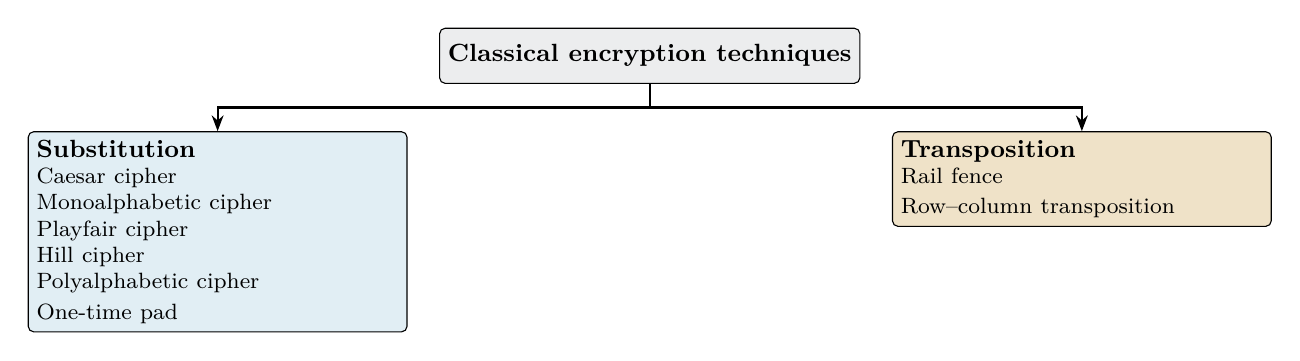
\begin{tikzpicture}[node distance=5mm]
  \node[box,fill=gray!15] (root) {\textbf{Classical encryption techniques}};
  \node[box,fill=cyan!10,below left=6mm and 4mm of root,text width=46mm,align=left] (sub) {\textbf{Substitution}\\
  \footnotesize Caesar cipher\\ \footnotesize Monoalphabetic cipher\\ \footnotesize Playfair cipher\\ \footnotesize Hill cipher\\ \footnotesize Polyalphabetic cipher\\ \footnotesize One-time pad};
  \node[box,fill=yellow!20,below right=6mm and 4mm of root,text width=46mm,align=left] (tra) {\textbf{Transposition}\\
  \footnotesize Rail fence\\ \footnotesize Row--column transposition};
  \draw[arr] (root.south) -- ++(0,-3mm) -| (sub.north);
  \draw[arr] (root.south) -- ++(0,-3mm) -| (tra.north);
\end{tikzpicture}
\end{center}

\section{Caesar Cipher}

\begin{keybox}
Earliest and simplest substitution cipher, used by Julius Caesar. Replace each letter with the letter \textbf{three places further down} the alphabet, wrapping from \ttx{z} back to \ttx{a}.
\end{keybox}

\subsection{Letters as numbers (start at 0)}
\begin{center}\small\setlength{\tabcolsep}{4pt}
\begin{tabular}{*{13}{c}}
\toprule
A&B&C&D&E&F&G&H&I&J&K&L&M\\
0&1&2&3&4&5&6&7&8&9&10&11&12\\
\midrule
N&O&P&Q&R&S&T&U&V&W&X&Y&Z\\
13&14&15&16&17&18&19&20&21&22&23&24&25\\
\bottomrule
\end{tabular}
\end{center}
Numbering from 0 matches the remainders mod 26, which are exactly $0,1,\dots,25$.

\subsection{Algorithm}
\begin{minipage}[c]{0.55\textwidth}
\begin{keybox}[title=Encryption and decryption]
\vspace{-6pt}
\begin{align*}
C &= E(p,k) = (p + k) \bmod 26\\
p &= D(C,k) = (C - k) \bmod 26
\end{align*}
Caesar cipher: $k = 3$.
\end{keybox}
\begin{itemize}
  \item $p$ = plaintext letter's number, $C$ = ciphertext letter's number, $k$ = key (shift).
  \item Convention: plaintext in lowercase, ciphertext in UPPERCASE.
  \item \textbf{mod gives the remainder, not the quotient.} $27 \bmod 26 = 1$.
  \item Negative during decryption? Add 26. \;$-2 \bmod 26 = 24$.
\end{itemize}
\end{minipage}\hfill
\begin{minipage}[c]{0.42\textwidth}
\centering
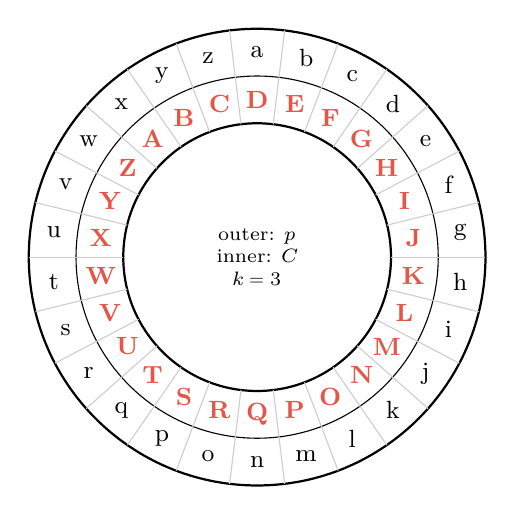
\begin{tikzpicture}
  \draw[thick] (0,0) circle (2.9);
  \draw (0,0) circle (2.3);
  \draw[thick] (0,0) circle (1.7);
  \foreach \pl/\cl [count=\n from 0] in {a/D,b/E,c/F,d/G,e/H,f/I,g/J,h/K,i/L,j/M,k/N,l/O,m/P,n/Q,o/R,p/S,q/T,r/U,s/V,t/W,u/X,v/Y,w/Z,x/A,y/B,z/C}{
    \pgfmathsetmacro{\ang}{90-\n*360/26}
    \pgfmathsetmacro{\sep}{\ang+180/26}
    \node[font=\small] at (\ang:2.6) {\pl};
    \node[font=\small\bfseries,text=warn] at (\ang:2.0) {\cl};
    \draw[gray!50] (\sep:1.7) -- (\sep:2.9);
  }
  \node[font=\scriptsize,align=center] at (0,0) {outer: $p$\\inner: $C$\\$k=3$};
\end{tikzpicture}
\end{minipage}

\subsection{Worked example: encrypt ``neso academy'' ($k=3$)}
\begin{center}\small\setlength{\tabcolsep}{5pt}
\begin{tabular}{@{}l*{4}{c}|*{7}{c}@{}}
\toprule
Plaintext & n&e&s&o & a&c&a&d&e&m&y\\
$p$ & 13&4&18&14 & 0&2&0&3&4&12&24\\
$p+3$ & 16&7&21&17 & 3&5&3&6&7&15&\hl{27}\\
$\bmod 26$ & 16&7&21&17 & 3&5&3&6&7&15&\hl{1}\\
Ciphertext & \textbf{Q}&\textbf{H}&\textbf{V}&\textbf{R} & \textbf{D}&\textbf{F}&\textbf{D}&\textbf{G}&\textbf{H}&\textbf{P}&\textbf{B}\\
\bottomrule
\end{tabular}
\end{center}
Answer: \textbf{\ttx{QHVR DFDGHPB}}.
The only wrap-around is \ttx{y}: $24+3 = 27$, and $27 = 26\times 1 + \mathbf{1}$, so $C = 1 = $ \ttx{B}.
(Counting on: y $\to$ z $\to$ a $\to$ \textbf{b}.) For the other letters you can just count three letters forward.

\subsection{Homework 1: decrypt ``QHWZRUN VHFXULWB'' ($k=3$)}
\begin{center}\small\setlength{\tabcolsep}{3.6pt}
\begin{tabular}{@{}l*{7}{c}|*{8}{c}@{}}
\toprule
Ciphertext & Q&H&W&Z&R&U&N & V&H&F&X&U&L&W&B\\
$C$ & 16&7&22&25&17&20&13 & 21&7&5&23&20&11&22&1\\
$C-3$ & 13&4&19&22&14&17&10 & 18&4&2&20&17&8&19&\hl{$-2$}\\
$\bmod 26$ & 13&4&19&22&14&17&10 & 18&4&2&20&17&8&19&\hl{24}\\
Plaintext & n&e&t&w&o&r&k & s&e&c&u&r&i&t&y\\
\bottomrule
\end{tabular}
\end{center}
Answer: \textbf{network security}. Note the last letter: $1-3=-2$, add 26 $\Rightarrow 24 =$ \ttx{y}.

\section{Shift Cipher (the general form)}

\begin{keybox}
Same formulas, but the key $k$ can be any of $1,2,\dots,25$. \textbf{Caesar cipher = shift cipher with $k=3$.}
\end{keybox}
\begin{itemize}
  \item $k=0$ is useless: $C = (p+0) \bmod 26 = p$, so the ciphertext equals the plaintext. (Homework: ``Neso'', $k=0$ $\Rightarrow$ \ttx{NESO}.)
  \item $k=26$ is the same as $k=0$. So there are only \textbf{25 usable keys}.
\end{itemize}

\textbf{Example:} ``Neso'', $k=4$: \;
N $13{+}4{=}17\to$\textbf{R},\;
e $4{+}4{=}8\to$\textbf{I},\;
s $18{+}4{=}22\to$\textbf{W},\;
o $14{+}4{=}18\to$\textbf{S} \;$\Rightarrow$\; \textbf{\ttx{RIWS}}.

\textbf{Homework 2:} ``cryptography'', $k=4$:
\begin{center}\small\setlength{\tabcolsep}{4.5pt}
\begin{tabular}{@{}l*{12}{c}@{}}
\toprule
Plaintext & c&r&y&p&t&o&g&r&a&p&h&y\\
$p$ & 2&17&24&15&19&14&6&17&0&15&7&24\\
$p+4 \bmod 26$ & 6&21&\hl{2}&19&23&18&10&21&4&19&11&\hl{2}\\
Ciphertext & G&V&C&T&X&S&K&V&E&T&L&C\\
\bottomrule
\end{tabular}
\end{center}
Answer: \textbf{\ttx{GVCTXSKVETLC}} (both \ttx{y}'s wrap: $24+4=28 \equiv 2$).

\textbf{In code:} the 0--25 numbering is a convention. With ASCII (\ttx{A}=65, \ttx{a}=97), shift to 0 first, then back:
\;$C = \big((p - 65 + k) \bmod 26\big) + 65$ for uppercase (use 97 for lowercase).

\subsection{Pros and cons of the Caesar cipher}
\begin{minipage}[t]{0.3\textwidth}
\textbf{Pros}
\begin{enumerate}[leftmargin=1.5em]
  \item Simple.
  \item Easy to implement.
\end{enumerate}
\end{minipage}\hfill
\begin{minipage}[t]{0.66\textwidth}
\textbf{Cons}
\begin{enumerate}[leftmargin=1.5em]
  \item The encryption and decryption algorithms are known.
  \item Only 25 keys to try $\Rightarrow$ vulnerable to \textbf{brute-force attack}.
  \item The plaintext language is known and easily recognisable, so you can tell when you have hit the right key.
\end{enumerate}
\end{minipage}

\section{Brute-Force Attack on the Caesar/Shift Cipher}

\begin{keybox}
\textbf{Brute force}: try every possible key until readable plaintext appears. With 25 keys this takes seconds by hand.
\end{keybox}

Ciphertext: \ttx{SQDYMZK}. Shift every letter forward by 0, 1, 2, \dots, 25 and look for a real word:

\begin{center}\small\ttfamily\setlength{\tabcolsep}{6pt}
\begin{tabular}{@{}ccl@{}}
\toprule
\rmfamily\bfseries Fwd & \rmfamily\bfseries Back & \rmfamily\bfseries Result\\
\midrule
0 & 26 & SQDYMZK\\
1 & 25 & TREZNAL\\
2 & 24 & USFAOBM\\
3 & 23 & VTGBPCN\\
4 & 22 & WUHCQDO\\
5 & 21 & XVIDREP\\
6 & 20 & YWJESFQ\\
7 & 19 & ZXKFTGR\\
8 & 18 & AYLGUHS\\
9 & 17 & BZMHVIT\\
10 & 16 & CANIWJU\\
11 & 15 & DBOJXKV$^\ast$\\
12 & 14 & ECPKYLW\\
\bottomrule
\end{tabular}
\qquad
\begin{tabular}{@{}ccl@{}}
\toprule
\rmfamily\bfseries Fwd & \rmfamily\bfseries Back & \rmfamily\bfseries Result\\
\midrule
13 & 13 & FDQLZMX\\
\rowcolor{warn!18} \textbf{14} & \textbf{12} & \textbf{GERMANY}\\
15 & 11 & HFSNBOZ\\
16 & 10 & IGTOCPA\\
17 & 9 & JHUPDQB\\
18 & 8 & KIVQERC\\
19 & 7 & LJWRFSD\\
20 & 6 & MKXSGTE\\
21 & 5 & NLYTHUF\\
22 & 4 & OMZUIVG$^\ast$\\
23 & 3 & PNAVJWH\\
24 & 2 & QOBWKXI\\
25 & 1 & RPCXLYJ\\
\bottomrule
\end{tabular}
\end{center}
{\footnotesize $^\ast$ Recomputed; the notes had these rows slightly wrong (see corrections box).}

\begin{itemize}
  \item Forward $+$ back $= 26$, because shifting forward 14 is the same as shifting back 12: $\;C + 14 \equiv C - 12 \pmod{26}$.
  \item Only one row is English: \textbf{GERMANY}. The attacker now has the plaintext \emph{and} the key.
  \item \textbf{Which number is the key?} The sender encrypted with $k = \mathbf{12}$ (G $6+12=18=$ S, \dots, Y $24+12=36\equiv10=$ K). The 14 is the forward shift that \emph{undoes} it. The lecture calls 14 ``the key''; be clear which one you mean in an exam.
\end{itemize}

\begin{keybox}[title=Decryption vs.\ cryptanalysis]
\textbf{Decryption}: the receiver \emph{has} the key and reverses the encryption.\\
\textbf{Cryptanalysis}: an attacker \emph{without} the key recovers the plaintext and/or the key (e.g.\ by brute force).
\end{keybox}

\begin{examtip}
\begin{itemize}
  \item Substitution = replace letters; transposition = rearrange letters. Know the list of ciphers under each.
  \item Write both formulas: $C=(p+k)\bmod 26$, $p=(C-k)\bmod 26$. Caesar is $k=3$.
  \item Always show the wrap-around step (e.g.\ $27 \bmod 26 = 1$) and fix negatives by adding 26.
  \item Key space is 25 (not 26): $k=0$ changes nothing.
  \item Three cons of Caesar: algorithms known, only 25 keys, language recognisable.
  \item For brute force: draw the table, box the readable row, state the key.
\end{itemize}
\end{examtip}

\begin{fixbox}
\begin{itemize}
  \item ``neso academy'' encrypts to \ttx{QHVR DFDGHPB}. The notes' final answer \ttx{QHVRDFDGHB} drops the \ttx{P}.
  \item Brute-force table: row 11 is \ttx{DBOJXKV} and row 22 is \ttx{OMZUIVG}. Row 12 (\ttx{ECPKYLW}) was already correct.
  \item The notes call con \#1 a ``Kerckhoffs violation''. It isn't: public algorithms are normal (see the intro sheet). The problem is a public algorithm \emph{plus} only 25 keys.
  \item Slide typo: ``used \emph{be} Julius Caesar'' $\to$ ``used \emph{by}''.
\end{itemize}
\end{fixbox}

% Videos: monoalphabetic ciphers, Playfair part 1 & 2, Playfair solved question
\newcommand{\NESOACADEMY}{{N,E,S,O,A},{C,D,M,Y,B},{F,G,H,{I/J},K},{L,P,Q,R,T},{U,V,W,X,Z}}
\newcommand{\JUPITER}{{{I/J},U,P,T,E},{R,A,B,C,D},{F,G,H,K,L},{M,N,O,Q,S},{V,W,X,Y,Z}}
\newcommand{\NESOAPP}{{N,E,S,O,A},{P,B,C,D,F},{G,H,{I/J},K,L},{M,Q,R,T,U},{V,W,X,Y,Z}}

\section{Monoalphabetic Cipher}

\textbf{Why:} Caesar shifts every letter by the \emph{same} amount, and there are only 25 keys. Find the shift for one letter and you have the whole message.

\subsection{Permutations}
\begin{keybox}
A \textbf{permutation} of a finite set $S$ is an ordered sequence of all the elements of $S$, with \textbf{each element appearing exactly once}.
\end{keybox}
$S=\{a,b,c\}$ has $3! = 6$ permutations: \ttx{abc, acb, bac, bca, cab, cba}.\quad
In general $n$ elements have $n! = n(n-1)\cdots 2\cdot 1$ permutations ($2! = 2$, $4! = 24$).

\subsection{The cipher}
\begin{keybox}
The ``cipher'' line can be \textbf{any permutation of the 26 letters}. Each plaintext letter always maps to the same ciphertext letter, and no two plaintext letters share a ciphertext letter.
\end{keybox}
\begin{itemize}
  \item Key space: $26! \approx 4 \times 10^{26}$ keys. This \emph{seems} to rule out brute force (compare 25 for Caesar).
  \item It is still a \textbf{substitution} cipher. The permutation is applied to the \emph{alphabet} (to build the key), not to the message (that would be transposition).
\end{itemize}

\textbf{Example:} ``Neso'' $\to$ \ttx{DULA}. The distance moved differs for every letter, so one letter's mapping tells you nothing about the others:
\begin{center}\small\setlength{\tabcolsep}{6pt}
\begin{tabular}{@{}lcccc@{}}
\toprule
Plaintext & N (13) & E (4) & S (18) & O (14)\\
Ciphertext & \textbf{D} (3) & \textbf{U} (20) & \textbf{L} (11) & \textbf{A} (0)\\
Shift $(C-p) \bmod 26$ & 16 & 16 & 19 & 12\\
\bottomrule
\end{tabular}
\qquad Caesar: shift is always 3.
\end{center}

\subsection{Breaking it: frequency analysis}
Letters in English are \textbf{not equally common}. A monoalphabetic cipher only renames letters, so the ciphertext keeps the same frequency pattern.
\begin{center}
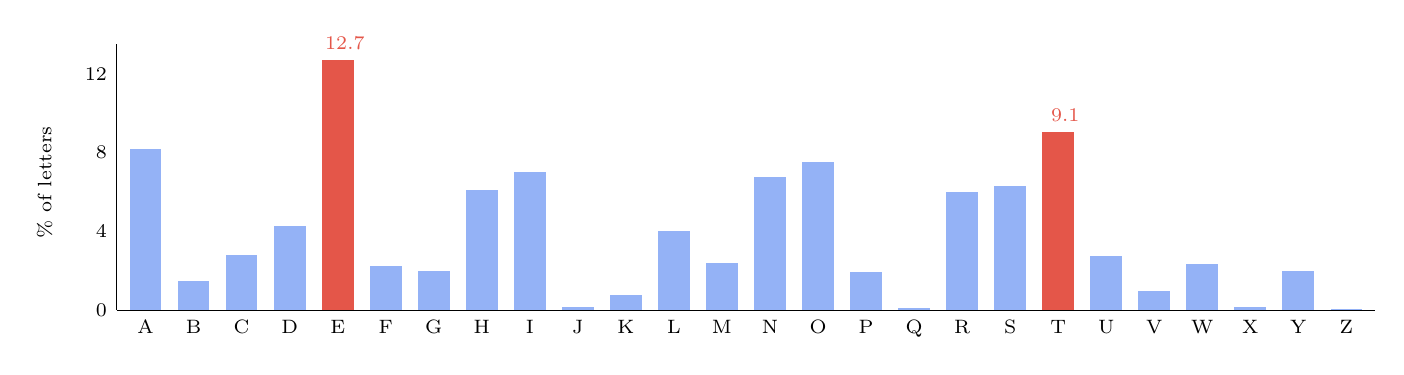
\begin{tikzpicture}[x=6.1mm,y=2.5mm]
  \foreach \L/\v [count=\i] in {A/8.167,B/1.492,C/2.782,D/4.253,E/12.702,F/2.228,G/2.015,H/6.094,I/6.996,J/0.153,K/0.772,L/4.025,M/2.406,N/6.749,O/7.507,P/1.929,Q/0.095,R/5.987,S/6.327,T/9.056,U/2.758,V/0.978,W/2.360,X/0.150,Y/1.974,Z/0.074}{
    \fill[acc!55] (\i-0.33,0) rectangle (\i+0.33,\v);
    \node[font=\scriptsize,below] at (\i,0) {\L};
  }
  \fill[warn] (5-0.33,0) rectangle (5.33,12.702) node[above,font=\scriptsize,xshift=-1.1mm] {12.7};
  \fill[warn] (20-0.33,0) rectangle (20.33,9.056) node[above,font=\scriptsize,xshift=-1.1mm] {9.1};
  \draw (0.4,0) -- (26.6,0);
  \draw (0.4,0) -- (0.4,13.5);
  \foreach \y in {0,4,8,12} \node[font=\scriptsize,left] at (0.4,\y) {\y};
  \node[font=\scriptsize,rotate=90] at (-1.1,6.5) {\% of letters};
\end{tikzpicture}
\end{center}
Most common: \textbf{E} (12.7\%), \textbf{T} (9.1\%), then A, O, I, N, S, H, R. Rarest: J, X, Q, Z.

\textbf{Method:} count ciphertext letters $\to$ the most frequent one is probably \ttx{e}, the next \ttx{t} $\to$ look for common words (\ttx{the}, \ttx{that}) and fill in the rest by guessing.

\textbf{Lecture example} (120 letters):
\begin{center}\small\ttfamily
UZQSOVUOHXMOPVGPOZPEVSGZWSZOPFPESXUDBMETSXAIZ\\
VUEPHZHMDZSHZOWSFPAPPDTSVPQUZWYMXUZUHSX\\
EPYEPOPDZSZUFPOMBZWPFUPZHMDJUDTMOHMQ
\end{center}
\begin{enumerate}[leftmargin=1.5em]
  \item Count: \ttx{P} appears 16 times (13.33\%), \ttx{Z} 14 times (11.67\%). Guess \ttx{P}$=$e, \ttx{Z}$=$t.
  \item \ttx{ZW} shows up 3 times and \ttx{ZWP} appears once: t?e $\Rightarrow$ ``the'', so \ttx{W}$=$h.
  \item Keep guessing with common words until it reads as English:
\end{enumerate}
\begin{center}\small
\emph{it was disclosed yesterday that several informal but direct contacts have been made with political representatives of the viet cong in moscow}
\end{center}
Recovered key (cipher $\to$ plain):
\begin{center}\small\setlength{\tabcolsep}{2.6pt}
\begin{tabular}{@{}l*{21}{c}@{}}
\toprule
Cipher & A&B&D&E&F&G&H&I&J&M&O&\textbf{P}&Q&S&T&U&V&\textbf{W}&X&Y&\textbf{Z}\\
Plain  & b&f&n&r&v&y&c&u&g&o&s&\textbf{e}&w&a&m&i&d&\textbf{h}&l&p&\textbf{t}\\
\bottomrule
\end{tabular}
\end{center}

\subsection{Pros, cons, countermeasure}
\begin{minipage}[t]{0.3\textwidth}
\textbf{Pros}
\begin{enumerate}[leftmargin=1.5em]
  \item Better security than Caesar cipher.
\end{enumerate}
\end{minipage}\hfill
\begin{minipage}[t]{0.66\textwidth}
\textbf{Cons}
\begin{enumerate}[leftmargin=1.5em]
  \item Easy to break because the ciphertext reflects the frequency data of the original alphabet.
  \item Prone to guessing attacks using English letter frequencies.
\end{enumerate}
\end{minipage}

\textbf{Countermeasure: homophones.} Give a common letter several possible substitutes (e.g.\ \ttx{e} gets many symbols, picked at random each time). This flattens the frequency peaks.

\subsection{Homework: encrypt with a key phrase}
Key: ``The quick brown fox jumps over the lazy dog''. Drop spaces and every repeated letter. It uses all 26 letters, so it becomes the whole cipher line:
\begin{center}\small\setlength{\tabcolsep}{2.4pt}
\begin{tabular}{@{}l*{26}{c}@{}}
\toprule
Plain & a&b&c&d&e&f&g&h&i&j&k&l&m&n&o&p&q&r&s&t&u&v&w&x&y&z\\
Cipher & T&H&E&Q&U&I&C&K&B&R&O&W&N&F&X&J&M&P&S&V&L&A&Z&Y&D&G\\
\bottomrule
\end{tabular}
\end{center}
``Attack postponed to tomorrow and do not use our secret paper until further info'' $\to$
\begin{center}\small\ttfamily
TVVTEO JXSVJXFUQ VX VXNXPPXZ TFQ QX FXV LSU XLP SUEPUV JTJUP LFVBW ILPVKUP BFIX
\end{center}
(Check one: a$\to$T, t$\to$V, t$\to$V, a$\to$T, c$\to$E, k$\to$O $\Rightarrow$ \ttx{TVVTEO}.)

\section{Playfair Cipher}\label{sec:playfair}

\begin{itemize}
  \item Also called the Playfair square or Wheatstone--Playfair cipher. A manual \textbf{symmetric} technique.
  \item \textbf{Invented} in 1854 by \textbf{Charles Wheatstone}; named after \textbf{Lord Playfair}, who \textbf{promoted} it.
  \item The first literal \textbf{digram} substitution cipher: it encrypts \textbf{two letters at a time}.
\end{itemize}

\begin{keybox}[title=Single-letter vs.\ multiple-letter]
Caesar and monoalphabetic: a letter always becomes the \emph{same} ciphertext letter.\\
Playfair: a letter's ciphertext depends on its \emph{partner} in the pair, so the same letter can become different letters. Single-letter frequencies are hidden.
\end{keybox}

\subsection{Building the 5$\times$5 key matrix}
\begin{minipage}[c]{0.6\textwidth}
\begin{enumerate}[leftmargin=1.5em]
  \item Write the keyword row by row, \textbf{skipping repeated letters}.
  \item Fill the remaining cells with the unused letters \textbf{in alphabetical order}.
  \item 26 letters, 25 cells: \textbf{I and J share one cell}. If the keyword contains I or J, that cell is already used.
\end{enumerate}
Keyword \textbf{MONARCHY} (highlighted), then B, D, E, F, G, I/J, K, L, P, Q, S, T, U, V, W, X, Z.
\end{minipage}\hfill
\begin{minipage}[c]{0.36\textwidth}
\centering
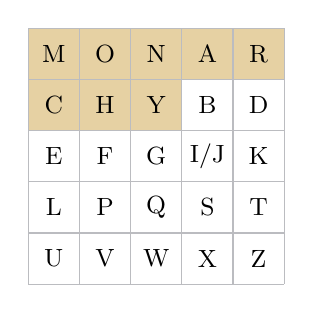
\begin{tikzpicture}[x=6.5mm,y=6.5mm]
  \foreach \c in {1,...,5}{\pfcell{\c}{1}{yellow!35}}
  \foreach \c in {1,2,3}{\pfcell{\c}{2}{yellow!35}}
  \pfletters{\MONARCHY}
\end{tikzpicture}
\end{minipage}

\subsection{Step 1: split the plaintext into digrams}
\begin{itemize}
  \item Split into pairs. \textbf{Two identical letters in one pair} $\Rightarrow$ insert filler \ttx{x} between them and re-pair from there.
  \item \textbf{Odd letter left over} at the end $\Rightarrow$ add filler \ttx{x}.
\end{itemize}
\begin{center}\small
\begin{tabular}{@{}lll@{}}
\toprule
Plaintext & Digrams & Why\\
\midrule
attack & \ttx{at ta ck} & nothing to fix (\ttx{tt} is split across two pairs)\\
neso academy & \ttx{ne so ac ad em yx} & 11 letters: \ttx{y} is left over, add \ttx{x}\\
balloon & \ttx{ba lx lo on} & \ttx{ll} in one pair: \ttx{l x}, then re-pair \ttx{l o o n}\\
\bottomrule
\end{tabular}
\end{center}

\subsection{Step 2: encrypt each pair (three cases)}
\begin{keybox}[title=Encryption rules]
\begin{enumerate}[leftmargin=1.5em]
  \item \textbf{Same row}: take the letter to the \textbf{right} of each (wrap to the start of the row).
  \item \textbf{Same column}: take the letter \textbf{below} each (wrap to the top).
  \item \textbf{Rectangle} (different row and column): each letter is replaced by the letter \textbf{in its own row}, in the \textbf{other letter's column}. Order matters: \ttx{at}$\to$\ttx{RS} but \ttx{ta}$\to$\ttx{SR}.
\end{enumerate}
\end{keybox}

\begin{center}
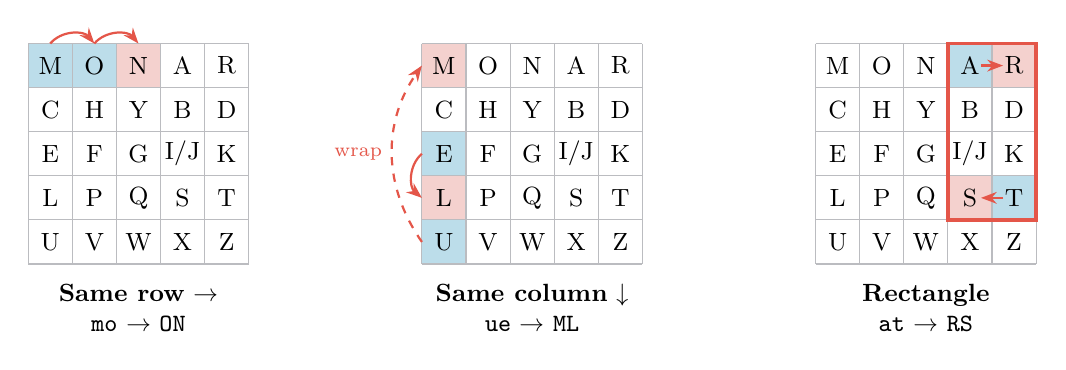
\begin{tikzpicture}[x=5.6mm,y=5.6mm]
  % same row: mo -> ON
  \begin{scope}
    \pfcell{1}{1}{cyan!25}\pfcell{2}{1}{cyan!25}\pfcell{3}{1}{warn!25}
    \pfletters{\MONARCHY}
    \draw[arr,warn] (0.5,0) to[bend left=50] (1.5,0);
    \draw[arr,warn] (1.5,0) to[bend left=50] (2.5,0);
    \node[font=\small,align=center] at (2.5,-6) {\textbf{Same row} $\to$\\\ttx{mo} $\to$ \ttx{ON}};
  \end{scope}
  % same column: ue -> ML
  \begin{scope}[xshift=50mm]
    \pfcell{1}{3}{cyan!25}\pfcell{1}{5}{cyan!25}\pfcell{1}{4}{warn!25}\pfcell{1}{1}{warn!25}
    \pfletters{\MONARCHY}
    \draw[arr,warn] (0,-2.5) to[bend right=50] (0,-3.5);
    \draw[arr,warn,dashed] (0,-4.5) to[bend left=35] node[left,font=\scriptsize]{wrap} (0,-0.5);
    \node[font=\small,align=center] at (2.5,-6) {\textbf{Same column} $\downarrow$\\\ttx{ue} $\to$ \ttx{ML}};
  \end{scope}
  % rectangle: at -> RS
  \begin{scope}[xshift=100mm]
    \pfcell{4}{1}{cyan!25}\pfcell{5}{4}{cyan!25}\pfcell{5}{1}{warn!25}\pfcell{4}{4}{warn!25}
    \pfletters{\MONARCHY}
    \draw[very thick,warn] (3,0) rectangle (5,-4);
    \draw[arr,warn] (3.75,-0.5) -- (4.25,-0.5);
    \draw[arr,warn] (4.25,-3.5) -- (3.75,-3.5);
    \node[font=\small,align=center] at (2.5,-6) {\textbf{Rectangle}\\\ttx{at} $\to$ \ttx{RS}};
  \end{scope}
\end{tikzpicture}\\[2pt]
{\footnotesize blue = plaintext pair, red = ciphertext}
\end{center}

\subsection{Worked examples (keyword MONARCHY)}
\begin{minipage}[t]{0.48\textwidth}
\textbf{``attack''} $\to$ \ttx{at ta ck}
\begin{itemize}
  \item \ttx{at}: rectangle $\to$ \ttx{RS}
  \item \ttx{ta}: rectangle $\to$ \ttx{SR}
  \item \ttx{ck}: rectangle (C row 2, K row 3) $\to$ \ttx{DE}
\end{itemize}
Answer: \textbf{\ttx{RSSRDE}}
\end{minipage}\hfill
\begin{minipage}[t]{0.48\textwidth}
\textbf{``mosque''} $\to$ \ttx{mo sq ue}
\begin{itemize}
  \item \ttx{mo}: same row $\to$ \ttx{ON}
  \item \ttx{sq}: same row $\to$ \ttx{TS}
  \item \ttx{ue}: same column, U wraps to top $\to$ \ttx{ML}
\end{itemize}
Answer: \textbf{\ttx{ONTSML}}
\end{minipage}

\medskip
\textbf{Rapid fire:}
\begin{center}\small\setlength{\tabcolsep}{5pt}
\begin{tabular}{@{}l*{8}{c}@{}}
\toprule
Digram & \ttx{oa} & \ttx{ab} & \ttx{gk} & \ttx{dc} & \ttx{rz} & \ttx{zr} & \ttx{mz} & \ttx{rm}\\
Case & row & column & row & row & column & column & rectangle & row\\
Wrap? & & & K$\to$E & D$\to$C & Z$\to$R & Z$\to$R & & R$\to$M\\
Answer & \textbf{NR} & \textbf{BI} & \textbf{IE} & \textbf{CH} & \textbf{DR} & \textbf{RD} & \textbf{RU} & \textbf{MO}\\
\bottomrule
\end{tabular}
\end{center}
(\ttx{BI}/\ttx{IE}: the I/J cell can be written as I or J.)

\subsection{Solved question}
\textbf{Encrypt ``Hide the gold under the carpet'' with keyword ``Neso Academy''.}

\begin{minipage}[c]{0.36\textwidth}
\centering
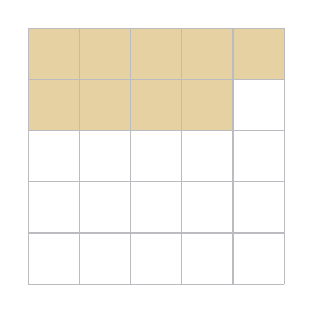
\begin{tikzpicture}[x=6.5mm,y=6.5mm]
  \foreach \c in {1,...,5}{\pfcell{\c}{1}{yellow!35}}
  \foreach \c in {1,...,4}{\pfcell{\c}{2}{yellow!35}}
  \pfletters{\NESOACADEMY}
\end{tikzpicture}\\[2pt]
{\footnotesize Keyword letters: N E S O A C D M Y}
\end{minipage}\hfill
\begin{minipage}[c]{0.6\textwidth}
25 letters (odd), so the last \ttx{t} gets a filler \ttx{x}. No pair has a repeated letter.\\[3pt]
\ttx{hi de th eg ol du nd er th ec ar pe tx}\\[3pt]
\small
\begin{tabular}{@{}lll|lll@{}}
\toprule
Pair & Case & Out & Pair & Case & Out\\
\midrule
hi & row & IK & er & rect. & OP\\
de & column & GD & th & rect. & QK\\
th & rect. & QK & ec & rect. & ND\\
eg & column & DP & ar & rect. & OT\\
ol & rect. & NR & pe & column & VD\\
du & rect. & CV & tx & rect. & RZ\\
nd & rect. & EC & & &\\
\bottomrule
\end{tabular}
\end{minipage}

\medskip
Answer: \textbf{\ttx{IKGDQKDPNRCVECOPQKNDOTVDRZ}}

The plaintext \ttx{e} became \ttx{D} (in \ttx{de}, \ttx{eg}, \ttx{pe}), \ttx{O} (in \ttx{er}) and \ttx{N} (in \ttx{ec}). That is the multiple-letter property.
But the same \emph{pair} always gives the same output (\ttx{th}$\to$\ttx{QK} both times). \emph{(Not in the lecture: this is why Playfair can still be attacked using pair frequencies.)}

\subsection{When I or J is in the keyword or the message}
\begin{keybox}[title=I/J rules]
\begin{itemize}
  \item I and J share one cell, so \textbf{replace every J with I before you do anything else}.
  \item In the \textbf{keyword}: a J takes the I/J cell. A later I (or J) in the keyword is then a \textbf{repeat}, so skip it.
  \item In the \textbf{message}: after the swap, \ttx{ij} or \ttx{ji} becomes \ttx{ii}, which is a \textbf{double letter} and needs a filler.
  \item The ciphertext never contains J; the cell is written as I. The receiver uses context to decide between i and j.
\end{itemize}
\end{keybox}

\textbf{Example:} encrypt ``meet me in fiji'' with keyword \textbf{JUPITER}.

\begin{minipage}[c]{0.36\textwidth}
\centering
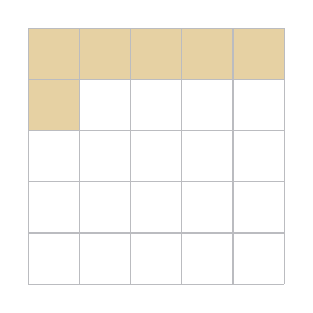
\begin{tikzpicture}[x=6.5mm,y=6.5mm]
  \foreach \c in {1,...,5}{\pfcell{\c}{1}{yellow!35}}
  \pfcell{1}{2}{yellow!35}
  \pfletters{\JUPITER}
\end{tikzpicture}\\[2pt]
{\footnotesize Keyword: J U P \sout{I} T E R}
\end{minipage}\hfill
\begin{minipage}[c]{0.6\textwidth}
\textbf{Matrix:} J goes into the first cell as I/J. The I in ``JUPITER'' is a repeat of that cell, so it is skipped. Then come U P T E R and the rest of the alphabet.

\textbf{Digrams:} \ttx{meetmeinfiji} $\to$ swap J: \ttx{meetmeinfi\underline{i}i}
\begin{itemize}
  \item \ttx{me et}: the \ttx{ee} is split across two pairs, so \textbf{no filler}.
  \item \ttx{fi}, then \ttx{ii} (was \ttx{ji}) is a double: \ttx{ix}, then the last \ttx{i} is alone: \ttx{ix}.
\end{itemize}
\ttx{me et me in fi ix ix}
\end{minipage}

\begin{center}\small
\begin{tabular}{@{}llll|llll@{}}
\toprule
Pair & Case & & Out & Pair & Case & & Out\\
\midrule
me & rectangle & & SI & fi & column & F$\to$M, I$\to$R & MR\\
et & row & E wraps to I & IE & ix & rectangle & I$\to$P, X$\to$V & PV\\
me & rectangle & & SI & ix & rectangle & & PV\\
in & rectangle & I$\to$U, N$\to$M & UM & & & &\\
\bottomrule
\end{tabular}
\end{center}
Ciphertext: \textbf{\ttx{SIIESIUMMRPVPV}}.\quad
Decrypting gives \ttx{me et me in fi ix ix}. Drop the fillers to get ``meet me in fiii''; context says \textbf{meet me in fiji}.

\subsection{Decryption}
\begin{keybox}[title=Reverse the rules]
Same row $\Rightarrow$ move \textbf{left}.\quad Same column $\Rightarrow$ move \textbf{up}.\quad Rectangle $\Rightarrow$ \textbf{same} rule as encryption. Then drop the filler \ttx{x}'s.
\end{keybox}

\textbf{Homework:} decrypt \ttx{ODZFQSEZSONTSW} with keyword ``Neso App''.

\begin{minipage}[c]{0.36\textwidth}
\centering
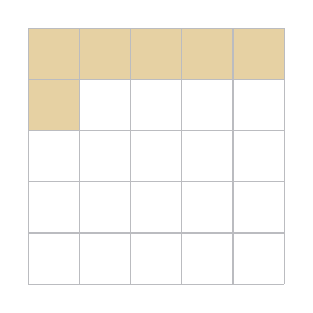
\begin{tikzpicture}[x=6.5mm,y=6.5mm]
  \foreach \c in {1,...,5}{\pfcell{\c}{1}{yellow!35}}
  \pfcell{1}{2}{yellow!35}
  \pfletters{\NESOAPP}
\end{tikzpicture}\\[2pt]
{\footnotesize Keyword letters: N E S O A P}
\end{minipage}\hfill
\begin{minipage}[c]{0.6\textwidth}
\small
\begin{tabular}{@{}lll@{}}
\toprule
Pair & Case & Plain\\
\midrule
OD & column (up; O wraps to bottom) & yo\\
ZF & column (up) & ua\\
QS & rectangle & re\\
EZ & rectangle & aw\\
SO & row (left) & es\\
NT & rectangle & om\\
SW & rectangle & ex\\
\bottomrule
\end{tabular}
\end{minipage}

\medskip
\ttx{yo ua re aw es om ex} $\to$ drop the filler $\to$ \textbf{you are awesome}.

\begin{examtip}
\begin{itemize}
  \item Monoalphabetic key space is $26!$; Caesar's is 25. A bigger key space still falls to \textbf{frequency analysis}.
  \item Know E and T are the most frequent English letters; know what homophones are for.
  \item Playfair: inventor \textbf{Wheatstone} (1854), promoter \textbf{Lord Playfair}. It is a \textbf{digram} (multiple-letter) cipher.
  \item Matrix: keyword without repeats, then the rest of the alphabet, I/J in one cell. Always draw it.
  \item Fix digrams \emph{before} encrypting: split doubled letters with \ttx{x}, pad an odd length with \ttx{x}.
  \item Row $\to$ right, column $\to$ down (with wrap), rectangle $\to$ own row, other's column. Decrypt: left, up, rectangle unchanged.
\end{itemize}
\end{examtip}

\begin{fixbox}
\begin{itemize}
  \item \textbf{Frequency example:} Gemini's copy of the ciphertext has an extra \ttx{Z}. The correct text (above) has 120 letters, with \ttx{P} 16 times and \ttx{Z} 14 times (the notes said 131 letters, \ttx{P} 18 times). In the notes, the step ``\ttx{S} = h, \ttx{ZSZ} = that'' is wrong: \ttx{W} = h (from \ttx{ZWP} = the) and \ttx{S} = a.
  \item \textbf{Short frequency example} (``\ttx{GZGEWVGRNCP}'' $\to$ ``we execute plan'') is left out. The letters in the notes don't produce that sentence (11 letters vs.\ 13, and the given mapping yields ``ewexcteplan''). Check the video at 11:08 if you need it.
  \item Neso App homework: \ttx{F}$\to$\ttx{A} is not a wrap (F is in row 2). Only \ttx{O}$\to$\ttx{Y} wraps.
  \item Video 3 (about 08:00): the speaker says ``W'' / ``MW'' but means \ttx{O} / \ttx{mo}. The slide is right: \ttx{mo}$\to$\ttx{ON}.
  \item Not covered in the video: if the filler itself would double (e.g.\ \ttx{xx}), a different filler such as \ttx{q} or \ttx{z} is normally used.
\end{itemize}
\end{fixbox}

% Videos: Hill cipher encryption, Hill cipher decryption, Vigenere & autokey, Vernam
\section{Hill Cipher}

\begin{itemize}
  \item A \textbf{multiletter} substitution cipher by mathematician \textbf{Lester Hill (1929)}. Better security than Playfair.
  \item Encrypts a \textbf{block of $m$ letters at a time} using an $m\times m$ \textbf{key matrix} $K$: $2\times2$ for digraphs, $3\times3$ for trigraphs, $m\times m$ for polygraphs.
  \item Like Playfair, the same letter can become different ciphertext letters depending on its block.
  \item Maths needed: matrix multiplication mod 26 (enough for encryption); \textbf{determinant} and \textbf{multiplicative inverse} mod 26 (needed for decryption).
\end{itemize}

\begin{keybox}[title=Hill cipher]
\vspace{-6pt}
\[
\text{Encrypt: } C = PK \bmod 26 \qquad\qquad \text{Decrypt: } P = CK^{-1} \bmod 26
\]
Works because $CK^{-1} = (PK)K^{-1} = P(KK^{-1}) = PI = P$.
\end{keybox}

For $m = 3$, the plaintext block is a \textbf{row vector} $(P_1\;P_2\;P_3)$:
\[
(C_1\;C_2\;C_3) = (P_1\;P_2\;P_3)\begin{pmatrix}K_{11}&K_{12}&K_{13}\\K_{21}&K_{22}&K_{23}\\K_{31}&K_{32}&K_{33}\end{pmatrix} \bmod 26
\qquad
\begin{aligned}
C_1 &= (P_1K_{11}+P_2K_{21}+P_3K_{31}) \bmod 26\\
C_2 &= (P_1K_{12}+P_2K_{22}+P_3K_{32}) \bmod 26\\
C_3 &= (P_1K_{13}+P_2K_{23}+P_3K_{33}) \bmod 26
\end{aligned}
\]
Sizes: $(1\times3)(3\times3) = (1\times3)$. Each $C_j$ = plaintext row $\cdot$ column $j$ of $K$.

\textbf{$PK$ vs.\ $KP$:} this lecture uses $C = PK$ (plaintext as a row). Some books use a \textbf{column} vector: $C = KP$, and then decryption is $P = K^{-1}C$. Use one convention consistently.

\subsection{Encryption example: ``pay more money''}
\[
K = \begin{pmatrix}17&17&5\\21&18&21\\2&2&19\end{pmatrix}
\qquad\text{Blocks of 3: } \ttx{pay | mor | emo | ney} \quad\text{(pad with \ttx{x} if needed)}
\]
Block 1, \ttx{pay} $= (15\;0\;24)$:
\[
\begin{aligned}
C_1 &= 15\cdot17 + 0\cdot21 + 24\cdot2 = 255+0+48 = 303 = 11\cdot26 + \mathbf{17} &&\to \ttx{R}\\
C_2 &= 15\cdot17 + 0\cdot18 + 24\cdot2 = 255+0+48 = 303 \equiv \mathbf{17} &&\to \ttx{R}\\
C_3 &= 15\cdot5 + 0\cdot21 + 24\cdot19 = 75+0+456 = 531 = 20\cdot26 + \mathbf{11} &&\to \ttx{L}
\end{aligned}
\]
\begin{center}\small
\begin{tabular}{@{}lcccc@{}}
\toprule
Block & $P$ & $PK$ (before mod) & $\bmod 26$ & Ciphertext\\
\midrule
pay & (15, 0, 24) & (303, 303, 531) & (17, 17, 11) & \textbf{RRL}\\
mor & (12, 14, 17) & (532, 490, 677) & (12, 22, 1) & \textbf{MWB}\\
emo & (4, 12, 14) & (348, 312, 538) & (10, 0, 18) & \textbf{KAS}\\
ney & (13, 4, 24) & (353, 341, 605) & (15, 3, 7) & \textbf{PDH}\\
\bottomrule
\end{tabular}
\end{center}
Answer: \textbf{\ttx{RRLMWBKASPDH}}.

\subsection{Decryption: finding $K^{-1}$}
\begin{keybox}[title=Recipe]
$K^{-1} = \big(\det K\big)^{-1} \cdot \operatorname{adj}(K) \bmod 26$
\begin{enumerate}[leftmargin=1.5em]
  \item $\det K \bmod 26$.
  \item Its multiplicative inverse mod 26.
  \item $\operatorname{adj}(K) \bmod 26$.
  \item Multiply (2) by (3), reduce mod 26. Check $KK^{-1} \equiv I$.
\end{enumerate}
\end{keybox}

\textbf{Step 1: determinant} (expand along row 1, signs $+\,-\,+$):
\[
\det K = 17\begin{vmatrix}18&21\\2&19\end{vmatrix} - 17\begin{vmatrix}21&21\\2&19\end{vmatrix} + 5\begin{vmatrix}21&18\\2&2\end{vmatrix}
= 17(300) - 17(357) + 5(6) = 5100 - 6069 + 30 = -939
\]
$-939 = -36\cdot26 - 3$, so $\det K \equiv -3 \equiv -3 + 26 = \mathbf{23} \pmod{26}$.

\textbf{Step 2: inverse of 23 mod 26.} Find $x$ with $23x \bmod 26 = 1$ by trying $x = 1, 2, 3, \dots$
\begin{center}\small\setlength{\tabcolsep}{3.2pt}
\begin{tabular}{@{}l*{17}{c}@{}}
\toprule
$x$ & 1&2&3&4&5&6&7&8&9&10&11&12&13&14&15&16&\hl{17}\\
$23x \bmod 26$ & 23&20&17&14&11&8&5&2&25&22&19&16&13&10&7&4&\hl{1}\\
\bottomrule
\end{tabular}
\end{center}
$23 \times 17 = 391 = 15\cdot26 + 1$, so $\mathbf{23^{-1} \equiv 17}$.
An inverse exists only if $\gcd(\det K, 26) = 1$, i.e.\ $\det K$ is odd and not 13. Otherwise the key can't be used, because messages could not be decrypted.

\textbf{Step 3: adjoint, using the $5\times5$ shortcut.}
\begin{enumerate}[leftmargin=1.5em]
  \item Copy the first two columns to the right, then the first two rows to the bottom ($5\times5$).
  \item Delete the first row and first column. That leaves a $4\times4$ grid.
  \item Slide a $2\times2$ window over the grid. Each window gives $ad - bc$.
  \textbf{Columns 1--2 of the grid give row 1 of $\operatorname{adj}K$} (windows at rows 1--2, 2--3, 3--4); columns 2--3 give row 2; columns 3--4 give row 3. The signs come out automatically.
\end{enumerate}
\begin{center}\small
\begin{tabular}{ccccc}
\color{gray}17&\color{gray}17&\color{gray}5&\color{gray}17&\color{gray}17\\
\color{gray}21&18&21&21&18\\
\color{gray}2&2&19&2&2\\
\color{gray}17&17&5&17&17\\
\color{gray}21&18&21&21&18
\end{tabular}
\quad$\Rightarrow$\quad
\begin{tabular}{|cc|cc|}
\hline
\cellcolor{cyan!20}18&\cellcolor{cyan!20}21&21&18\\
\cellcolor{cyan!20}2&\cellcolor{cyan!20}19&2&2\\
17&5&17&17\\
18&21&21&18\\
\hline
\end{tabular}
\quad
{\footnotesize first window: $18\cdot19 - 21\cdot2 = 300$}
\end{center}
\[
\operatorname{adj}K =
\begin{pmatrix}
18\cdot19-21\cdot2 & 2\cdot5-19\cdot17 & 17\cdot21-5\cdot18\\
21\cdot2-21\cdot19 & 19\cdot17-2\cdot5 & 5\cdot21-17\cdot21\\
21\cdot2-18\cdot2 & 2\cdot17-2\cdot17 & 17\cdot18-17\cdot21
\end{pmatrix}
=
\begin{pmatrix}300&-313&267\\-357&313&-252\\6&0&-51\end{pmatrix}
\]
\[
\equiv
\begin{pmatrix}14&-1&7\\-19&1&-18\\6&0&-25\end{pmatrix}
\equiv
\begin{pmatrix}14&25&7\\7&1&8\\6&0&1\end{pmatrix} \pmod{26}
\]
(Reduce mod 26, then add 26 to each negative: $-1\to25$, $-19\to7$, $-18\to8$, $-25\to1$.)

\textbf{Step 4: combine.}
\[
K^{-1} = 17\begin{pmatrix}14&25&7\\7&1&8\\6&0&1\end{pmatrix}
= \begin{pmatrix}238&425&119\\119&17&136\\102&0&17\end{pmatrix}
\equiv \boxed{\begin{pmatrix}4&9&15\\15&17&6\\24&0&17\end{pmatrix}} \pmod{26}
\]
Check: $KK^{-1} = \begin{pmatrix}443&442&442\\858&495&780\\494&52&365\end{pmatrix} \equiv \begin{pmatrix}1&0&0\\0&1&0\\0&0&1\end{pmatrix} = I$ \checkmark\;
($443 = 17\cdot26+1$, $442 = 17\cdot26$, \dots)

\subsection{Decryption example: \ttx{RRLMWBKASPDH}}
\begin{center}\small
\begin{tabular}{@{}lcccc@{}}
\toprule
Block & $C$ & $CK^{-1}$ (before mod) & $\bmod 26$ & Plaintext\\
\midrule
RRL & (17, 17, 11) & (587, 442, 544) & (15, 0, 24) & \textbf{pay}\\
MWB & (12, 22, 1) & (402, 482, 329) & (12, 14, 17) & \textbf{mor}\\
KAS & (10, 0, 18) & (472, 90, 456) & (4, 12, 14) & \textbf{emo}\\
PDH & (15, 3, 7) & (273, 186, 362) & (13, 4, 24) & \textbf{ney}\\
\bottomrule
\end{tabular}
\end{center}
e.g.\ $P_1 = 17\cdot4 + 17\cdot15 + 11\cdot24 = 68 + 255 + 264 = 587 = 22\cdot26 + 15 \to \ttx{p}$.\quad Answer: \textbf{pay more money}.

{\small\emph{Not in the lecture:} Hill hides single-letter frequencies well, but it is linear. If an attacker knows some plaintext--ciphertext pairs, they can solve for $K$.}

\section{Polyalphabetic Ciphers}\label{sec:poly}

Monoalphabetic ciphers fall to frequency analysis because every letter always gets the same substitute. \textbf{Polyalphabetic} ciphers use \textbf{different} monoalphabetic rules at different positions:
\begin{keybox}
\begin{enumerate}[leftmargin=1.5em]
  \item A \textbf{set of related monoalphabetic substitution rules} is used.
  \item A \textbf{key} decides which rule is used for each letter.
\end{enumerate}
\end{keybox}

\subsection{Vigen\`ere cipher}
The rule set is the \textbf{26 Caesar ciphers} (shifts 0--25). Each key letter picks the shift for one plaintext letter. The key is \textbf{repeated} to the length of the message.
\begin{keybox}[title=Vigen\`ere (key length $m$)]
\vspace{-6pt}
\[
C_i = \big(P_i + K_{i \bmod m}\big) \bmod 26 \qquad\qquad P_i = \big(C_i - K_{i \bmod m}\big) \bmod 26
\]
\end{keybox}

\textbf{Example:} plaintext \ttx{wearediscoveredsaveyourself} (27 letters), key \ttx{deceptive} (9 letters, repeated 3 times).
\begin{center}\footnotesize\setlength{\tabcolsep}{2.9pt}
\begin{tabular}{@{}l*{14}{c}@{}}
\toprule
Key & d&e&c&e&p&t&i&v&e&d&e&c&e&p\\
$K$ & 3&4&2&4&15&19&8&21&4&3&4&2&4&15\\
Plain & w&e&a&r&e&d&i&s&c&o&v&e&r&e\\
$P$ & 22&4&0&17&4&3&8&18&2&14&21&4&17&4\\
$(P{+}K) \bmod 26$ & 25&8&2&21&19&22&16&\hl{13}&6&17&25&6&21&19\\
Cipher & \textbf{Z}&\textbf{I}&\textbf{C}&\textbf{V}&\textbf{T}&\textbf{W}&\textbf{Q}&\textbf{N}&\textbf{G}&\textbf{R}&\textbf{Z}&\textbf{G}&\textbf{V}&\textbf{T}\\
\bottomrule
\end{tabular}
\\[4pt]
\begin{tabular}{@{}l*{13}{c}@{}}
\toprule
Key & t&i&v&e&d&e&c&e&p&t&i&v&e\\
$K$ & 19&8&21&4&3&4&2&4&15&19&8&21&4\\
Plain & d&s&a&v&e&y&o&u&r&s&e&l&f\\
$P$ & 3&18&0&21&4&24&14&20&17&18&4&11&5\\
$(P{+}K) \bmod 26$ & 22&\hl{0}&21&25&7&\hl{2}&16&24&\hl{6}&\hl{11}&12&\hl{6}&9\\
Cipher & \textbf{W}&\textbf{A}&\textbf{V}&\textbf{Z}&\textbf{H}&\textbf{C}&\textbf{Q}&\textbf{Y}&\textbf{G}&\textbf{L}&\textbf{M}&\textbf{G}&\textbf{J}\\
\bottomrule
\end{tabular}
\end{center}
Answer: \textbf{\ttx{ZICVTWQNGRZGVTWAVZHCQYGLMGJ}} (highlighted cells wrapped past 25).

\textbf{Why it's stronger:} the same plaintext letter gets different ciphertext letters. \ttx{e} at position 2 (key \ttx{e}=4) $\to 8 =$ \ttx{I}; \ttx{e} at position 5 (key \ttx{p}=15) $\to 19 =$ \ttx{T}. Letter frequencies get flattened.

\textbf{Cryptanalysis:} the weakness is that the \textbf{key repeats}. Once the attacker finds the key length $m$, they split the ciphertext into $m$ groups (every $m$-th letter). Each group is just a \textbf{Caesar cipher}, which falls to frequency analysis or brute force.

\subsection{Autokey system}
To stop the key from repeating, Vigen\`ere proposed the \textbf{autokey}: the keyword is followed by the \textbf{plaintext itself}, giving a \textbf{running key} as long as the message.
\begin{center}\small\ttfamily\setlength{\tabcolsep}{2.2pt}
\begin{tabular}{@{}l*{27}{c}@{}}
\rmfamily Key & \textbf{d}&\textbf{e}&\textbf{c}&\textbf{e}&\textbf{p}&\textbf{t}&\textbf{i}&\textbf{v}&\textbf{e}&w&e&a&r&e&d&i&s&c&o&v&e&r&e&d&s&a&v\\
\rmfamily Plain & w&e&a&r&e&d&i&s&c&o&v&e&r&e&d&s&a&v&e&y&o&u&r&s&e&l&f\\
\rmfamily Cipher & Z&I&C&V&T&W&Q&N&G&K&Z&E&I&I&G&A&S&X&S&T&S&L&V&V&W&L&A
\end{tabular}
\end{center}
Answer: \textbf{\ttx{ZICVTWQNGKZEIIGASXSTSLVVWLA}}. The first 9 letters match Vigen\`ere (same key); after that the key is the plaintext (\ttx{w e a r e \dots}).
\begin{itemize}
  \item No period to find, so the key-length attack above fails.
  \item Still breakable: the key is ordinary English too, so key and plaintext \textbf{share the same letter frequencies}, and statistics can still be applied.
\end{itemize}

\subsection{Vernam cipher}
\begin{itemize}
  \item \textbf{Gilbert Vernam}, AT\&T engineer, \textbf{1918}.
  \item Works on \textbf{binary bits}, not letters.
  \item Goal: a key \textbf{as long as the message} that \textbf{does not repeat}, so no statistical pattern is left.
\end{itemize}
\begin{minipage}[c]{0.5\textwidth}
\begin{keybox}[title=Vernam]
\vspace{-6pt}
\[
C_i = P_i \oplus K_i \qquad\qquad P_i = C_i \oplus K_i
\]
$\oplus$ = XOR: output 1 if the bits differ, 0 if they are equal.
\end{keybox}
Decryption works because XOR undoes itself:
\[
C_i \oplus K_i = P_i \oplus K_i \oplus K_i = P_i \oplus 0 = P_i
\]
\end{minipage}\hfill
\begin{minipage}[c]{0.45\textwidth}
\centering\small
\begin{tabular}{cc|c}
\toprule
$a$ & $b$ & $a\oplus b$\\
\midrule
0&0&0\\ 0&1&1\\ 1&0&1\\ 1&1&0\\
\bottomrule
\end{tabular}
\qquad
\begin{tabular}{@{}r@{\;}l@{}}
$P$ & \ttx{1011}\\
$K$ & \ttx{0110}\\
\midrule
$C$ & \ttx{1101}\\
$C\oplus K$ & \ttx{1011} $= P$
\end{tabular}\\[2pt]
{\footnotesize (bit example is mine, not from the lecture)}
\end{minipage}

\begin{center}
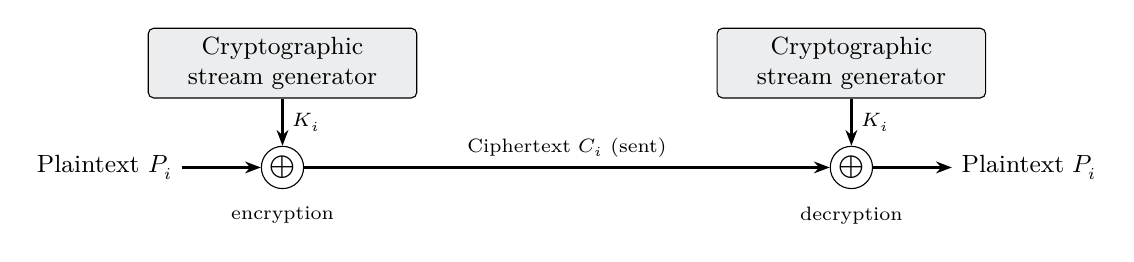
\begin{tikzpicture}[node distance=6mm]
  \node[box,fill=gray!15,text width=32mm] (g1) {Cryptographic stream generator};
  \node[draw,circle,below=6mm of g1,font=\large,inner sep=1pt] (x1) {$\oplus$};
  \node[left=10mm of x1,font=\small] (p1) {Plaintext $P_i$};
  \node[box,fill=gray!15,text width=32mm,right=38mm of g1] (g2) {Cryptographic stream generator};
  \node[draw,circle,below=6mm of g2,font=\large,inner sep=1pt] (x2) {$\oplus$};
  \node[right=10mm of x2,font=\small] (p2) {Plaintext $P_i$};
  \draw[arr] (g1) -- node[right,font=\scriptsize]{$K_i$} (x1);
  \draw[arr] (g2) -- node[right,font=\scriptsize]{$K_i$} (x2);
  \draw[arr] (p1) -- (x1);
  \draw[arr] (x1) -- node[above,font=\scriptsize]{Ciphertext $C_i$ (sent)} (x2);
  \draw[arr] (x2) -- (p2);
  \node[below=1mm of x1,font=\scriptsize] {encryption};
  \node[below=1mm of x2,font=\scriptsize] {decryption};
\end{tikzpicture}
\end{center}
Both sides need the \textbf{same, synchronised key stream}.

\textbf{Weakness:} Vernam's machine read the key from a \textbf{loop of paper tape}, so the key eventually \textbf{repeated}. With enough ciphertext, and some known or probable plaintext, it can be broken.
\textbf{Fix:} make the key truly random, as long as the message, and never reused. That is the \textbf{one-time pad}, which gives perfect secrecy (next topic).

\begin{examtip}
\begin{itemize}
  \item Hill: $C = PK \bmod 26$, $P = CK^{-1} \bmod 26$. State which convention ($PK$ or $KP$) you use.
  \item $K^{-1} = (\det K)^{-1}\operatorname{adj}K \bmod 26$. Show every step: det, inverse (table), adjoint, product, then check $KK^{-1}=I$.
  \item Negative numbers mod 26: add 26 until the result is in $0$--$25$.
  \item The key matrix must have $\gcd(\det K, 26) = 1$, or it can't be inverted.
  \item Polyalphabetic = many monoalphabetic rules, and the key picks which one. Vigen\`ere = 26 Caesar ciphers.
  \item Vigen\`ere weakness: the repeating key. Autokey fixes it (keyword + plaintext), but key and plaintext share frequencies.
  \item Vernam: Gilbert Vernam, 1918, bits, XOR. Weakness: repeating tape. Leads to the one-time pad.
\end{itemize}
\end{examtip}

\begin{fixbox}
\begin{itemize}
  \item All of Gemini's numbers for this batch are correct (Hill encryption, det, adjoint, $K^{-1}$, decryption, Vigen\`ere, autokey; checked by script).
  \item Slide typos noted by Gemini: for \ttx{ney}, the slide shows the old vector $(348, 312, 538)$ instead of $(353, 341, 605)$. For \ttx{RRL}, the slide shows $(17\;17\;14)$ labelled $C$; it should be $(17\;17\;11)$ and the output is $P$.
  \item The notes put ``key and plaintext share letter frequencies'' under Vigen\`ere cryptanalysis. That point is really about the autokey system, where the key \emph{is} plaintext, so it is placed there above.
\end{itemize}
\end{fixbox}

% Videos: one-time pad, rail fence, row column transposition
\newcommand{\railfence}[1]{%
  \foreach \l/\r [count=\i] in {#1}{\node[font=\small] (rf\i) at (\i*0.5,-\r*0.6) {\l};}}

\section{One-Time Pad}\label{sec:otp}

The last substitution technique. It is an \textbf{improvement to the Vernam cipher}:
\begin{keybox}[title=One-time pad]
\begin{itemize}
  \item The key is \textbf{random} and \textbf{as long as the message}, so it never repeats.
  \item The key is used to encrypt and decrypt \textbf{a single message}, then \textbf{discarded}. Each new message needs a new key of the same length.
  \item Such a scheme is \textbf{unbreakable}: ``the ultimate in security''.
\end{itemize}
\end{keybox}

\subsection{How it grew out of the earlier ciphers}
\begin{center}\small
\begin{tabularx}{\textwidth}{@{}l X X@{}}
\toprule
Cipher & Key & What goes wrong\\
\midrule
Vigen\`ere & short keyword, \textbf{repeated} & repeats every $m$ letters $\Rightarrow$ split into Caesar ciphers\\
Autokey & keyword + plaintext & key is English $\Rightarrow$ has English letter frequencies\\
Vernam & long key stream (paper tape) & tape loops, so the key \textbf{eventually repeats}\\
\textbf{One-time pad} & \textbf{truly random}, \textbf{same length} as message, \textbf{used once} & nothing to exploit\\
\bottomrule
\end{tabularx}
\end{center}
The OTP is a Vigen\`ere/Vernam cipher whose key \emph{never} repeats and has \emph{no} pattern. The formulas don't change:
\[
C_i = (P_i + K_i) \bmod 26,\quad P_i = (C_i - K_i) \bmod 26 \quad\text{(letters)}\qquad\qquad C_i = P_i \oplus K_i,\quad P_i = C_i \oplus K_i \quad\text{(bits)}
\]

\subsection{Example 1: letters}
Plaintext \ttx{attackatdawn}, random key \ttx{qvhzmxkbplwe} (12 letters for 12 letters):
\begin{center}\small\setlength{\tabcolsep}{4.5pt}
\begin{tabular}{@{}l*{12}{c}@{}}
\toprule
Plain & a&t&t&a&c&k&a&t&d&a&w&n\\
$P$ & 0&19&19&0&2&10&0&19&3&0&22&13\\
Key & q&v&h&z&m&x&k&b&p&l&w&e\\
$K$ & 16&21&7&25&12&23&10&1&15&11&22&4\\
$P+K$ & 16&\hl{40}&\hl{26}&25&14&\hl{33}&10&20&18&11&\hl{44}&17\\
$\bmod 26$ & 16&14&0&25&14&7&10&20&18&11&18&17\\
Cipher & \textbf{Q}&\textbf{O}&\textbf{A}&\textbf{Z}&\textbf{O}&\textbf{H}&\textbf{K}&\textbf{U}&\textbf{S}&\textbf{L}&\textbf{S}&\textbf{R}\\
\bottomrule
\end{tabular}
\end{center}
Ciphertext \textbf{\ttx{QOAZOHKUSLSR}}. The receiver computes $(C - K) \bmod 26$ letter by letter to get \ttx{attackatdawn} back, then destroys the key.
Note the two \ttx{t}'s in \ttx{att} became \ttx{O} and \ttx{A}. The two \ttx{S}'s in the ciphertext came from different letters (\ttx{d}, \ttx{w}).

\subsection{Example 2: bits}
``HI'' in 8-bit ASCII, XOR a random key:
\begin{center}\small\ttfamily
\begin{tabular}{@{}r@{\quad}l@{\quad}l@{}}
\rmfamily Plaintext (H, I) & 01001000 & 01001001\\
\rmfamily Key & 10110101 & 01101100\\
\midrule
\rmfamily Ciphertext $P\oplus K$ & 11111101 & 00100101\\
\rmfamily $C \oplus K$ & 01001000 & 01001001 \rmfamily\;= ``HI'' again\\
\end{tabular}
\end{center}

\subsection{Why it can't be broken}
\begin{itemize}
  \item It produces random output with \textbf{no statistical relationship to the plaintext}.
  \item The ciphertext contains \textbf{no information whatsoever} about the plaintext, so there is simply no way to break the code.
  \item The security comes \textbf{entirely from the randomness of the key}.
\end{itemize}

\textbf{Look at one letter.} The attacker sees \ttx{Q}. Every plaintext letter could have produced it, each with exactly one key letter:
\begin{center}\small\setlength{\tabcolsep}{5pt}
\begin{tabular}{@{}l*{7}{c}@{}}
\toprule
If the plaintext was & a & b & c & d & e & \dots & z\\
then the key was & q & p & o & n & m & \dots & r\\
\bottomrule
\end{tabular}
\end{center}
The key is random, so all 26 cases are \textbf{equally likely}. Seeing \ttx{Q} tells the attacker nothing.

\textbf{Look at the whole message.} The same ciphertext decrypts to anything of the same length, depending on the key:
\begin{center}\small
\begin{tabular}{@{}lll@{}}
\toprule
Ciphertext & Key tried & Result\\
\midrule
\ttx{QOAZOHKUSLSR} & \ttx{qvhzmxkbplwe} & \textbf{attack at dawn}\\
\ttx{QOAZOHKUSLSR} & \ttx{zkhikhruztku} & \textbf{retreat at six}\\
\ttx{KXFUDM} & \ttx{kemubc} & \textbf{attack}\\
\ttx{KXFUDM} & \ttx{htaqqj} & \textbf{defend}\\
\bottomrule
\end{tabular}
\end{center}
Brute force produces \emph{every} meaningful message of that length, and there is nothing to say which one is right. (Compare Caesar: only one of the 25 tries made sense, GERMANY.)

\subsection{The rules, and what breaks if you bend them}
\begin{keybox}[title=Rule 1: never reuse a key (the ``two-time pad'')]
Encrypt a second message \ttx{holdposition} with the \emph{same} key \ttx{qvhzmxkbplwe}: $C_2 = $ \ttx{XJSCBLCJITKR}.
\begin{itemize}
  \item Subtracting the ciphertexts cancels the key: $C_1 - C_2 = (P_1 + K) - (P_2 + K) = P_1 - P_2$ \;(\ttx{TFIXNWILKSIA} both ways). What's left is two English texts mixed together, which has structure the attacker can attack.
  \item Worse: if the attacker knows or guesses $P_1$ (``attack at dawn'' is a common phrase), then $K = C_1 - P_1 =$ \ttx{qvhzmxkbplwe}, and $P_2 = C_2 - K =$ \textbf{hold position}.
\end{itemize}
With bits it is the same: $C_1 \oplus C_2 = P_1 \oplus P_2$.
\end{keybox}
\begin{keybox}[title=Rule 2: the key must be truly random]
If the key is text from a book (a ``running key''), it has English letter frequencies, and it can be attacked like the autokey. If it comes from a formula or a short seed, it is really a stream cipher: at best \emph{computationally} secure, not perfect.
\end{keybox}
\begin{keybox}[title=Rule 3: the key must be at least as long as the message]
A shorter key has to repeat, and then you're back to Vigen\`ere/Vernam and their weaknesses.
\end{keybox}
\textbf{Known plaintext doesn't hurt an OTP.} If the attacker learns one plaintext and its ciphertext, they get $K = C - P$, but only for that message. That key is never used again.

\subsection{Two fundamental difficulties}
\begin{enumerate}[leftmargin=1.5em]
  \item \textbf{Making large quantities of random keys.} Every message needs fresh random key material of the same size.
  \item Even more daunting: \textbf{key distribution and protection}. Both sides need the same huge key, delivered and stored securely. (If you had a secure way to send that much key, you could send the message that way instead.)
\end{enumerate}
So the one-time pad is of \textbf{limited use}. It suits \textbf{low-bandwidth channels that need very high security}.

\subsection{Perfect secrecy}
\begin{keybox}
The one-time pad is the \textbf{only} cryptosystem with \textbf{perfect secrecy}: the ciphertext reveals \textbf{absolutely nothing} about the plaintext.
\end{keybox}
This is exactly the \textbf{unconditionally secure} idea from Section~\ref{sec:schemes}: no amount of ciphertext or computing power helps. (Formally, $P(\text{plaintext} \mid \text{ciphertext}) = P(\text{plaintext})$, a definition due to Shannon.)
Everything else in this course (AES, RSA, \dots) is only \textbf{computationally} secure: breaking it is possible in principle, just too slow or too costly.

\section{Transposition Ciphers}

\begin{keybox}
Some sort of \textbf{permutation} is applied to the plaintext letters. Letters are \textbf{not replaced}; only their \textbf{positions} change. The simplest such cipher is the \textbf{rail fence}.
\end{keybox}

\subsection{Rail fence}
Write the plaintext \textbf{down and up along diagonals} over $D$ rows (the \textbf{depth}), then \textbf{read off row by row}. Spaces and punctuation are dropped.

\textbf{Example:} ``neso academy is the best'', depth 2 (20 letters):
\begin{center}
\begin{tikzpicture}
  \railfence{n/0,e/1,s/0,o/1,a/0,c/1,a/0,d/1,e/0,m/1,y/0,i/1,s/0,t/1,h/0,e/1,b/0,e/1,s/0,t/1}
  \foreach \i in {1,...,19}{\pgfmathtruncatemacro{\j}{\i+1}\draw[gray!50] (rf\i) -- (rf\j);}
  \node[font=\scriptsize,anchor=east] at (0.2,0) {row 1};
  \node[font=\scriptsize,anchor=east] at (0.2,-0.6) {row 2};
\end{tikzpicture}
\end{center}
Row 1: \ttx{NSAAEYSHBS}\quad Row 2: \ttx{EOCDMITEET}\quad $\Rightarrow$\quad \textbf{\ttx{NSAAEYSHBSEOCDMITEET}}

\textbf{Depth 3}, ``Thank you very much'' (16 letters). The path goes 1, 2, 3, 2, 1, 2, 3, \dots\ (repeats every $2(D-1) = 4$ letters):
\begin{center}
\begin{tikzpicture}
  \railfence{t/0,h/1,a/2,n/1,k/0,y/1,o/2,u/1,v/0,e/1,r/2,y/1,m/0,u/1,c/2,h/1}
  \foreach \i in {1,...,15}{\pgfmathtruncatemacro{\j}{\i+1}\draw[gray!50] (rf\i) -- (rf\j);}
\end{tikzpicture}
\end{center}
Rows: \ttx{TKVM} + \ttx{HNYUEYUH} + \ttx{AORC} $\Rightarrow$ \textbf{\ttx{TKVMHNYUEYUHAORC}}

\textbf{Homework} (``neso academy is the best'', depth 3): rows \ttx{NAESB} + \ttx{EOCDMITEET} + \ttx{SAYHS}\\ $\Rightarrow$ \textbf{\ttx{NAESBEOCDMITEETSAYHS}}.

\subsection{Decrypting a rail fence}
The receiver knows the depth $D$. The problem is that they don't know where one row ends and the next begins in the ciphertext. So first work out \textbf{how many letters each row holds}.
\begin{keybox}[title={Rail fence decryption, step by step}]
\begin{enumerate}[leftmargin=1.5em]
  \item Count the letters $L$. The zig-zag pattern of rows repeats every $2(D-1)$ letters.
  \item Write the \textbf{row number of every position} (1, 2, \dots, $D$, \dots, 2, 1, 2, \dots) and \textbf{count} how many times each row appears.
  \item \textbf{Cut} the ciphertext into pieces of those lengths: the first piece is row 1, the next is row 2, and so on.
  \item Put each piece back into its row's positions, left to right. Then \textbf{read along the zig-zag} (position 1, 2, 3, \dots).
\end{enumerate}
\end{keybox}

\textbf{Example 1: depth 2.} \ttx{NSAAEYSHBSEOCDMITEET} (20 letters). Pattern 1 2 1 2 \dots\ so each row has 10 letters:
row 1 $=$ \ttx{NSAAEYSHBS}, row 2 $=$ \ttx{EOCDMITEET}. Take letters alternately from row 1 and row 2:
\ttx{N}\textbf{\ttx{E}}\ttx{S}\textbf{\ttx{O}}\ttx{A}\textbf{\ttx{C}}\dots\ $\Rightarrow$ \textbf{nesoacademyisthebest}.
(Depth-2 shortcut: split in half and interleave. With an odd length, row 1 gets the extra letter.)

\textbf{Example 2: depth 3.} \ttx{TKVMHNYUEYUHAORC} (16 letters). The pattern repeats every $2(3-1) = 4$:
\begin{center}\small\setlength{\tabcolsep}{4pt}
\begin{tabular}{@{}l*{16}{c}@{}}
\toprule
Position & 1&2&3&4&5&6&7&8&9&10&11&12&13&14&15&16\\
Row & 1&2&3&2&1&2&3&2&1&2&3&2&1&2&3&2\\
\bottomrule
\end{tabular}
\end{center}
Row 1 appears 4 times, row 2 8 times, row 3 4 times. Cut: \ttx{TKVM | HNYUEYUH | AORC}.
Fill the row-1 positions (1, 5, 9, 13) with T K V M, the row-2 positions with H N Y U E Y U H, and the row-3 positions with A O R C. Reading positions 1 to 16 gives \textbf{thankyouverymuch}.

\textbf{Example 3: depth 4, unequal rows} (the tricky case). \ttx{CGIRORYSYTAHFNPPU} (17 letters). The pattern repeats every $2(4-1) = 6$:
\begin{center}\small\setlength{\tabcolsep}{4pt}
\begin{tabular}{@{}l*{17}{c}@{}}
\toprule
Position & 1&2&3&4&5&6&7&8&9&10&11&12&13&14&15&16&17\\
Row & 1&2&3&4&3&2&1&2&3&4&3&2&1&2&3&4&3\\
\bottomrule
\end{tabular}
\end{center}
Counts: row 1 $= 3$, row 2 $= 5$, row 3 $= 6$, row 4 $= 3$ (total 17 \checkmark). Cut: \ttx{CGI | RORYS | YTAHFN | PPU}. Put the pieces back:
\begin{center}
\begin{tikzpicture}
  \railfence{C/0,R/1,Y/2,P/3,T/2,O/1,G/0,R/1,A/2,P/3,H/2,Y/1,I/0,S/1,F/2,U/3,N/2}
  \foreach \i in {1,...,16}{\pgfmathtruncatemacro{\j}{\i+1}\draw[gray!50] (rf\i) -- (rf\j);}
  \node[font=\scriptsize,anchor=east] at (0.2,0) {row 1: CGI};
  \node[font=\scriptsize,anchor=east] at (0.2,-0.6) {row 2: RORYS};
  \node[font=\scriptsize,anchor=east] at (0.2,-1.2) {row 3: YTAHFN};
  \node[font=\scriptsize,anchor=east] at (0.2,-1.8) {row 4: PPU};
\end{tikzpicture}
\end{center}
Read along the line: \textbf{cryptographyisfun} (``cryptography is fun'').
\emph{Trap:} don't assume the rows are equal, or that the middle rows are equal to each other. Here rows 2 and 3 have different lengths because the message stops partway through a cycle.

\textbf{Check yourself:} decrypt the homework answer \ttx{NAESBEOCDMITEETSAYHS} (depth 3). The counts are 5, 10, 5.

\subsection{Row--column transposition}
\begin{keybox}[title=A more complex scheme]
\textbf{Write} the message into a rectangle \textbf{row by row}. \textbf{Read} it \textbf{column by column}. The \textbf{key} is the \textbf{order of the columns}. Fill leftover cells with filler letters (e.g.\ \ttx{x y z}).
\end{keybox}

\textbf{Example:} ``Kill Corona Virus at twelve am tomorrow'' (33 letters), 7 columns $\times$ 5 rows = 35 cells, so 2 fillers (\ttx{y}, \ttx{z}). Key \textbf{4 3 1 2 5 6 7}.
\begin{center}\small
\begin{minipage}[c]{0.4\textwidth}\centering
\begin{tabular}{|*{7}{c|}}
\multicolumn{1}{c}{4}&\multicolumn{1}{c}{3}&\multicolumn{1}{c}{\textbf{1}}&\multicolumn{1}{c}{2}&\multicolumn{1}{c}{5}&\multicolumn{1}{c}{6}&\multicolumn{1}{c}{7}\\
\hline
k&i&\cellcolor{warn!18}l&l&c&o&r\\ \hline
o&n&\cellcolor{warn!18}a&v&i&r&u\\ \hline
s&a&\cellcolor{warn!18}t&t&w&e&l\\ \hline
v&e&\cellcolor{warn!18}a&m&t&o&m\\ \hline
o&r&\cellcolor{warn!18}r&o&w&\textit{y}&\textit{z}\\ \hline
\end{tabular}\\[2pt]
{\footnotesize numbers above = read order}
\end{minipage}
\begin{minipage}[c]{0.5\textwidth}
\begin{tabular}{@{}lll@{}}
\toprule
Order & Column & Letters\\
\midrule
1 & col 3 & LATAR\\
2 & col 4 & LVTMO\\
3 & col 2 & INAER\\
4 & col 1 & KOSVO\\
5 & col 5 & CIWTW\\
6 & col 6 & OREOY\\
7 & col 7 & RULMZ\\
\bottomrule
\end{tabular}
\end{minipage}
\end{center}
Answer: \textbf{\ttx{LATARLVTMOINAERKOSVOCIWTWOREOYRULMZ}}

\subsection{Two stages: more complex}
A single transposition leaves patterns that can be pieced back together. So \textbf{feed the ciphertext back in} and transpose again with the same key:
\begin{center}\small
\begin{minipage}[c]{0.4\textwidth}\centering
\begin{tabular}{|*{7}{c|}}
\multicolumn{1}{c}{4}&\multicolumn{1}{c}{3}&\multicolumn{1}{c}{\textbf{1}}&\multicolumn{1}{c}{2}&\multicolumn{1}{c}{5}&\multicolumn{1}{c}{6}&\multicolumn{1}{c}{7}\\
\hline
L&A&\cellcolor{warn!18}T&A&R&L&V\\ \hline
T&M&\cellcolor{warn!18}O&I&N&A&E\\ \hline
R&K&\cellcolor{warn!18}O&S&V&O&C\\ \hline
I&W&\cellcolor{warn!18}T&W&O&R&E\\ \hline
O&Y&\cellcolor{warn!18}R&U&L&M&Z\\ \hline
\end{tabular}
\end{minipage}
\begin{minipage}[c]{0.5\textwidth}
Read columns 3, 4, 2, 1, 5, 6, 7:\\[2pt]
\ttx{TOOTR AISWU AMKWY LTRIO RNVOL LAORM VECEZ}
\end{minipage}
\end{center}
Answer: \textbf{\ttx{TOOTRAISWUAMKWYLTRIORNVOLLAORMVECEZ}}.
The full key is now: the rectangle size, the column order and the number of stages.

{\small\emph{Decrypting (not shown in the lecture):} the receiver knows the rectangle size, so each column has 5 letters. Write the ciphertext \emph{into columns} in key order, then read the rows. For two stages, do this twice.}

\section{Classical Ciphers at a Glance}
\begin{center}\small
\begin{tabularx}{\textwidth}{@{}l l l X@{}}
\toprule
Cipher & Type & Key & Main weakness\\
\midrule
Caesar & substitution, 1 letter & shift 3 (fixed) & algorithm known, no real key\\
Shift & substitution, 1 letter & shift 1--25 & only 25 keys: brute force\\
Monoalphabetic & substitution, 1 letter & permutation ($26!$) & letter frequencies preserved\\
Playfair & substitution, 2 letters & 5$\times$5 keyword matrix & same pair $\to$ same output\\
Hill & substitution, $m$ letters & invertible $m\times m$ matrix & linear (known plaintext)\\
Vigen\`ere & polyalphabetic & repeating keyword & key repeats: split into Caesars\\
Autokey & polyalphabetic & keyword + plaintext & key has English frequencies\\
Vernam & polyalphabetic, bits (XOR) & key stream & tape key repeated\\
One-time pad & substitution & random, once, message length & none (perfect secrecy); key generation and distribution\\
Rail fence & transposition & depth & few possibilities\\
Row--column & transposition & column order (+ stages) & one stage can be reconstructed\\
\bottomrule
\end{tabularx}
\end{center}
Transposition ciphers keep the letter frequencies of the plaintext unchanged (only positions move).

\begin{examtip}
\begin{itemize}
  \item OTP: random key, same length as message, used once then discarded $\Rightarrow$ unbreakable, perfect secrecy.
  \item Reusing an OTP key: $C_1 - C_2 = P_1 - P_2$ (or $C_1\oplus C_2 = P_1\oplus P_2$), so the key cancels out. One known plaintext then reveals the other message.
  \item Know the two difficulties word for word: (1) making large quantities of random keys; (2) key distribution and protection.
  \item Substitution changes letters; transposition changes positions.
  \item Rail fence: draw the zig-zag, then read row by row. State the depth.
  \item Row--column: draw the grid with the key above it, pad the last row, and read columns in key order. Two stages = do it again on the ciphertext.
\end{itemize}
\end{examtip}

\begin{fixbox}
\begin{itemize}
  \item ``Thank you very much'', depth 3, is \ttx{TKVMHNYUEYUH}\textbf{\ttx{AORC}}. The notes' final string ends in \ttx{AORE}, but their own row reading gives \ttx{AORC}.
  \item Row--column: the speaker says ``R U L M C'' for column 7, but the grid (and slide) give \ttx{RULMZ}. All other results were checked by script and are correct.
  \item The OTP formulas, Shannon and $P(M\mid C) = P(M)$ come from Gemini's notes, not the slides. They are standard and correct.
\end{itemize}
\end{fixbox}

% College Lecture 5 topics not in the Neso videos: multiplicative/affine, cryptanalysis of Vigenere/Hill/affine, rotor, keyed transposition, stream vs block
\section{Traditional Ciphers: Remaining Topics (Lecture 5)}\label{sec:classextra}

\subsection{Multiplicative and affine ciphers}
\begin{center}\small
\begin{tabular}{@{}lll@{}}
\toprule
Cipher & Encrypt & Decrypt / key space\\
\midrule
Additive (shift) & $C = (P + k) \bmod 26$ & $P = (C - k) \bmod 26$; \; 26 keys\\
Multiplicative & $C = (P \times k) \bmod 26$ & $P = (C \times k^{-1}) \bmod 26$; \; $k \in \mathbb{Z}_{26}^*$: \textbf{12 keys}\\
Affine & $C = (P k_1 + k_2) \bmod 26$ & $P = ((C - k_2) k_1^{-1}) \bmod 26$; \; $12 \times 26 = \mathbf{312}$ keys\\
\bottomrule
\end{tabular}
\end{center}
$\mathbb{Z}_{26}^* = \{1, 3, 5, 7, 9, 11, 15, 17, 19, 21, 23, 25\}$ (odd and not 13).
\begin{itemize}
  \item Multiplicative, $k = 7$: \ttx{hello} $= 7, 4, 11, 11, 14 \to 49, 28, 77, 77, 98 \bmod 26 = 23, 2, 25, 25, 20 =$ \ttx{XCZZU}.
  \item Affine, $(k_1, k_2) = (7, 2)$: \ttx{hello} $\to$ \ttx{ZEBBW}. Decrypt with $7^{-1} = 15$: $(25 - 2) \cdot 15 = 345 \equiv 7 = h$, etc.
\end{itemize}

\textbf{Chosen-plaintext attack on affine} (slide example): Eve encrypts \ttx{et} on Alice's machine with two candidate algorithms and gets \ttx{WC} and \ttx{WF}.
\begin{itemize}
  \item \ttx{et}$\to$\ttx{WC}: $4k_1 + k_2 \equiv 22$, $19k_1 + k_2 \equiv 2$. Subtract: $15k_1 \equiv -20 \equiv 6$ $\Rightarrow k_1 = 16$: \textbf{rejected} ($\gcd(16, 26) \ne 1$).
  \item \ttx{et}$\to$\ttx{WF}: $15k_1 \equiv 5 - 22 \equiv 9$, $15^{-1} = 7$, $k_1 = 63 \bmod 26 = \mathbf{11}$, $k_2 = 22 - 44 \equiv \mathbf{4}$. Decrypting the intercepted text gives ``best time of the year is spring when flowers bloom''.
\end{itemize}

\subsection{Cryptanalysis of Vigen\`ere: the Kasiski test}
\begin{enumerate}[leftmargin=1.5em]
  \item Find repeated segments ($\ge 3$ letters) in the ciphertext; note the distances $d_1, d_2, \dots$
  \item The key length $m$ divides $\gcd(d_1, d_2, \dots)$.
  \item Split the ciphertext into $m$ interleaved pieces (letters $1, m{+}1, 2m{+}1, \dots$); each piece is a plain shift cipher, so break each by frequency analysis.
\end{enumerate}
Slide example: JSU (100), SUM (48), VWV (60), MPH (8): $\gcd = 4$ $\Rightarrow$ try $m = 4$. Each piece keeps single-letter frequencies even though the whole ciphertext doesn't.

\subsection{Cryptanalysis of Hill: known-plaintext}
Brute force is hopeless ($26^{m \times m}$ keys) and Hill hides single-letter, digram and trigram statistics. But with $m$ known plaintext/ciphertext blocks, stack them as rows of $P$ and $C$: since $C = PK$, \;$\boxed{K = P^{-1}C}$ (if $P$ is invertible mod 26; otherwise use other blocks).
\[
P = \begin{pmatrix}5&7&10\\13&17&7\\0&5&4\end{pmatrix},\;
C = \begin{pmatrix}3&6&0\\14&16&9\\3&17&11\end{pmatrix},\;
\det P \equiv 9,\;
P^{-1} = \begin{pmatrix}21&14&1\\0&8&25\\13&3&8\end{pmatrix},\;
K = P^{-1}C = \begin{pmatrix}2&3&7\\5&7&9\\1&2&11\end{pmatrix}
\]
(All entries mod 26, verified.)

\subsection{Rotor ciphers and Enigma}
A \textbf{rotor cipher} is a monoalphabetic substitution whose mapping \textbf{changes after every character} (the rotor turns one position). \textbf{Enigma} (Scherbius; German army, WWII): keyboard, plugboard, three rotors (slow, middle, fast) and a reflector; the wiring changes as you type.

\subsection{Transposition: keyless, keyed, combined}
\begin{itemize}
  \item \textbf{Keyless}: rail fence (\ttx{meetmeatthepark} $\to$ \ttx{MEMATEAKETETHPR}), or write row by row into 4 columns and read column by column ($\to$ \ttx{MMTAEEHREAEKTTP}).
  \item \textbf{Keyed (block) transposition}: split into blocks and permute each with the key. \ttx{enemy attac kston ightz}, encryption key \ttx{3 1 4 5 2} (output position $i$ takes input character key[$i$]) $\to$ \ttx{EEMYN TAACT TKONS HITZG}.
  \item \textbf{Keyed columnar (combined)}: write row by row, permute columns with the key, read column by column $\to$ \ttx{ETTHEAKIMAOTYCNZNTSG}.
  \item \textbf{Key inversion}: for each index $i$, \ttx{DecKey[EncKey[i]] = i}. Encryption key \ttx{3 1 4 5 2} $\to$ decryption key \ttx{2 5 1 3 4}; \;\ttx{2 6 3 1 4 7 5} $\to$ \ttx{4 1 3 5 7 2 6}.
  \item \textbf{As matrices}: the key is a permutation matrix (one 1 in each row and column); $C = PK$, and $K^{-1} = K^{T}$, so decryption just transposes the key matrix.
  \item \textbf{Cryptanalysis}: single-letter frequencies survive (statistical attack); brute force over $1! + 2! + \dots + L!$ keys, but the column count must divide $L$ ($L = 20 \Rightarrow 2, 4, 5, 10$); \textbf{pattern attack} on the regular position pattern (03 08 13 18 01 06 \dots). \textbf{Double transposition} (repeat the whole thing, usually with the same key) destroys the regular pattern.
\end{itemize}

\subsection{Stream vs.\ block ciphers}
\textbf{Stream}: one symbol at a time with a key stream, $c_i = E_{k_i}(p_i)$: additive, monoalphabetic, Vigen\`ere, OTP. \textbf{Block}: $m > 1$ symbols encrypted together with one key; each ciphertext block depends on the whole plaintext block: Playfair, Hill.

\begin{trap}[: Vigen\`ere is a stream cipher]
Even though the key repeats every $m$ letters, Vigen\`ere encrypts one character at a time, each with its own key element: a \textbf{stream} cipher. Playfair works on pairs, Hill on $m$-letter blocks: \textbf{block} ciphers.
\end{trap}

% Videos: steganography, LSB steganography demo, cryptography solved questions, abstract algebra & number theory intro, prime numbers
\definecolor{puregreen}{RGB}{0,255,0}
\definecolor{modgreen}{RGB}{0,252,0}

\section{Steganography}

\begin{keybox}
\textbf{Steganography} \textbf{conceals the existence} of the message: the message is hidden. It is \textbf{not an encryption scheme}.\\
\textbf{Cryptography} renders the message \textbf{unintelligible} to outsiders by transforming the text.
\end{keybox}
\begin{center}\small
\begin{tabularx}{\textwidth}{@{}l X X@{}}
\toprule
 & \textbf{Cryptography} & \textbf{Steganography}\\
\midrule
Hides & the \textbf{meaning} & the \textbf{existence}\\
Attacker sees & a scrambled message; knows something secret is being sent & an ordinary-looking text/image; doesn't suspect anything\\
Output & ciphertext & a normal-looking \textbf{cover} (text, image, audio) with the message inside\\
\bottomrule
\end{tabularx}
\end{center}
This is the other kind of ``security-related transformation $T$'' mentioned in the network security model (Section 1): $T$ doesn't have to be encryption.

\textbf{Examples from the lecture} (read the first letters):
\begin{itemize}
  \item \textbf{S}imply \textbf{e}ncrypt \textbf{c}orrect \textbf{r}eading \textbf{e}xactly \textbf{t}wice. $\Rightarrow$ \textbf{Secret}
  \item \textbf{T}ell \textbf{h}enry \textbf{a}lice \textbf{n}ot \textbf{k}ane / \textbf{Y}esterday \textbf{o}urplan \textbf{u}ndone! $\Rightarrow$ \textbf{Thank You}
\end{itemize}

\subsection{Historical techniques}
\begin{center}\small
\begin{tabularx}{\textwidth}{@{}l X@{}}
\toprule
Character marking & Chosen letters of a printed text are overwritten faintly in pencil. Visible only when the paper is held at an angle to bright light.\\
Invisible ink & Written with a substance (e.g.\ lemon juice) that leaves no trace until heat or a chemical is applied.\\
Pin punctures & Tiny pin holes on selected letters. Invisible until the paper is held up to a light.\\
Typewriter correction ribbon & Text typed between the lines with a correction ribbon. Visible only under strong light.\\
\bottomrule
\end{tabularx}
\end{center}

\subsection{Drawbacks}
\begin{enumerate}[leftmargin=1.5em]
  \item \textbf{Lots of overhead}: a large cover is needed to hide a few bits of message.
  \item \textbf{Once the system is discovered, it becomes virtually worthless}. Unlike encryption, there is no secret key left to protect the message.
\end{enumerate}
\begin{keybox}[title=Best of both]
A message can be \textbf{first encrypted and then hidden} using steganography. If the hiding is discovered, the attacker still only has ciphertext.
\end{keybox}
\begin{center}
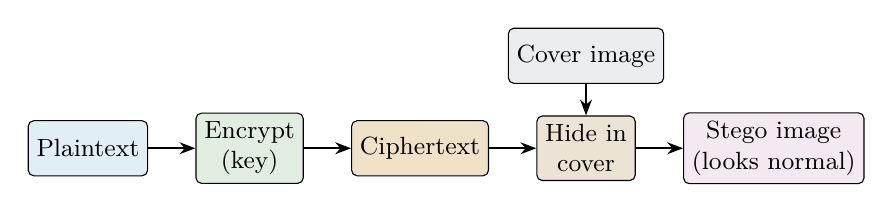
\begin{tikzpicture}[node distance=6mm]
  \node[box,fill=cyan!10] (p) {Plaintext};
  \node[box,fill=green!15,right=of p] (e) {Encrypt\\(key)};
  \node[box,fill=yellow!20,right=of e] (c) {Ciphertext};
  \node[box,fill=orange!15,right=of c] (h) {Hide in\\cover};
  \node[box,fill=gray!15,above=4mm of h] (cv) {Cover image};
  \node[box,fill=magenta!8,right=of h] (s) {Stego image\\(looks normal)};
  \draw[arr] (p)--(e); \draw[arr] (e)--(c); \draw[arr] (c)--(h); \draw[arr] (cv)--(h); \draw[arr] (h)--(s);
\end{tikzpicture}
\end{center}

\subsection{LSB steganography}
\textbf{LSB} = least significant bit(s): the rightmost bits of a number, which change its value the least.
\[
1010\,10\underbrace{01}_{\text{LSBs}} \qquad\text{bit weights: } 128\;64\;32\;16\;8\;4\;\underline{2\;1}
\]
\textbf{RGB model:} each pixel is 24 bits, 8 each for Red, Green and Blue (0--255).
\begin{center}\small Red $(255,0,0) = (\ttx{11111111}, \ttx{00000000}, \ttx{00000000})$ \quad Green $(0,255,0)$ \quad Blue $(0,0,255)$\end{center}

\begin{center}
\begin{tikzpicture}
  \fill[puregreen] (0,0) rectangle (3.2,1.4);
  \fill[modgreen] (4.2,0) rectangle (7.4,1.4);
  \node[font=\small,below] at (1.6,0) {$(0, 255, 0)$, G $=$ \ttx{111111\textbf{11}}};
  \node[font=\small,below] at (5.8,0) {$(0, 252, 0)$, G $=$ \ttx{111111\textbf{00}}};
\end{tikzpicture}
\end{center}
The two boxes look identical, but the last 2 bits differ. \textbf{Those LSBs can store hidden information.}
Using 2 LSBs in each of R, G and B hides $2 \times 3 = \mathbf{6}$ \textbf{bits per pixel}, and no channel value changes by more than 3.

\textbf{Worked example} (mine): hide the bits \ttx{11 01 10} in the pixel $(100, 50, 200)$:
\begin{center}\small
\begin{tabular}{@{}lllll@{}}
\toprule
Channel & Value & Binary & Replace last 2 bits & New value\\
\midrule
R & 100 & \ttx{011001\textbf{00}} & \ttx{011001\textbf{11}} & 103 ($+3$)\\
G & 50 & \ttx{001100\textbf{10}} & \ttx{001100\textbf{01}} & 49 ($-1$)\\
B & 200 & \ttx{110010\textbf{00}} & \ttx{110010\textbf{10}} & 202 ($+2$)\\
\bottomrule
\end{tabular}
\end{center}
To extract, the receiver just reads the last 2 bits of each channel. \textbf{Capacity:} an $800\times600$ image holds $800 \cdot 600 \cdot 6 = 2{,}880{,}000$ bits $= 360{,}000$ bytes.

\textbf{Blue orchids:} the lecture shows the image without and with hidden information side by side, and you can't tell them apart.

\subsection{Watermarking vs.\ image steganography}
\begin{center}\small
\begin{tabularx}{\textwidth}{@{}l X X@{}}
\toprule
 & \textbf{Watermarking} & \textbf{Image steganography}\\
\midrule
Purpose & prove \textbf{ownership} / copyright & \textbf{secret communication}\\
Is the mark secret? & no; it's often visible (like the \ttx{nesoacademy.org} logo) & yes; its \textbf{existence} is hidden\\
Hidden data & logo, owner info & any message or file\\
\bottomrule
\end{tabularx}
\end{center}

\subsection{OpenStego demo}
\begin{enumerate}[leftmargin=1.5em]
  \item \textbf{Hide Data:} message file \ttx{My Message.txt} (``Kill Corona Virus'', 17 bytes) + cover file \ttx{Blue Orchids.jpg} (58.4 KB) $\to$ stego file \ttx{BO.png} (824 KB). No password. ``Message embedded into 1 cover file(s).''
  \item \textbf{Extract Data:} input \ttx{BO.png} $\to$ output folder. ``Message file extracted successfully'', and the text file comes back unchanged.
\end{enumerate}
{\small\emph{Why PNG and why so much bigger (not explained in the video):} JPEG compression slightly changes pixel values, which would wipe out the LSBs. So the stego image is saved in the lossless PNG format, which is much larger. That size jump is itself a hint something is going on.}

\section{Solved Exam Questions}

\textbf{Q1.} Sender and receiver use the \textbf{same key}: \textbf{(b) private key} and \textbf{(c) symmetric} cryptography are both correct (two names for the same thing).

\textbf{Q2.} $19 \bmod 3$: $19 = 6 \cdot 3 + \mathbf{1}$, so the answer is \textbf{(d) 1}. (mod gives the remainder.)

\textbf{Q3 (UGC NET 2016).} An attacker captures information and \textbf{retransmits it later without altering it}. Options: DoS / masquerade / simple / complex. Official answer: \textbf{(a) denial of service}. Reason given: repeated retransmissions flood the receiver so it can't serve real users.
\begin{keybox}[title=Exam note]
The textbook name for ``capture and retransmit later'' is a \textbf{replay attack}. If \emph{replay} is one of the options, choose it. Here it isn't, so DoS is the best available answer.
\end{keybox}

\textbf{Q4 (ISRO 2020).} Columnar transposition, plaintext ``the tomato is a plant in the night shade family'', keyword \textbf{TOMATO}.
38 letters, 6 columns $\Rightarrow$ 7 rows (42 cells), 4 fillers \ttx{x}. Number the keyword letters alphabetically; \textbf{for repeated letters, go left to right}:
\begin{center}\small
\begin{minipage}[c]{0.4\textwidth}\centering
\begin{tabular}{|*{6}{c|}}
\multicolumn{1}{c}{T}&\multicolumn{1}{c}{O}&\multicolumn{1}{c}{M}&\multicolumn{1}{c}{A}&\multicolumn{1}{c}{T}&\multicolumn{1}{c}{O}\\
\multicolumn{1}{c}{5}&\multicolumn{1}{c}{3}&\multicolumn{1}{c}{2}&\multicolumn{1}{c}{\textbf{1}}&\multicolumn{1}{c}{6}&\multicolumn{1}{c}{4}\\
\hline
t&h&e&\cellcolor{warn!18}t&o&m\\\hline
a&t&o&\cellcolor{warn!18}i&s&a\\\hline
p&l&a&\cellcolor{warn!18}n&t&i\\\hline
n&t&h&\cellcolor{warn!18}e&n&i\\\hline
g&h&t&\cellcolor{warn!18}s&h&a\\\hline
d&e&f&\cellcolor{warn!18}a&m&i\\\hline
l&y&\textit{x}&\cellcolor{warn!18}\textit{x}&\textit{x}&\textit{x}\\\hline
\end{tabular}
\end{minipage}
\begin{minipage}[c]{0.5\textwidth}
Read order A, M, O, O, T, T $=$ columns 4, 3, 2, 6, 1, 5:\\[3pt]
\ttx{TINESAX EOAHTFX HTLTHEY MAIIAIX TAPNGDL OSTNHMX}\\[3pt]
Answer: \textbf{(a)}.\\[2pt]
{\footnotesize (The slide gave both O's the number 3 and both T's the number 4, then read left to right. That is the same order.)}
\end{minipage}
\end{center}

\textbf{Q5 (GATE 2015).} $N$ people, every pair needs its own \textbf{symmetric} key that nobody else knows. One key per pair:
\[
\binom{N}{2} = \frac{N(N-1)}{2} \qquad (N=2: 1,\; N=3: 3,\; N=4: 6,\; N=5: 10) \qquad\text{Answer: \textbf{(c)}}
\]
{\small\emph{Common follow-up (not in the video):} with \textbf{public-key} cryptography, each person needs just one key pair: $N$ pairs, $2N$ keys in total. This is one big reason public-key cryptography exists.}

\section{Prime Numbers}
\begin{keybox}
\textbf{Prime}: $> 1$ with exactly two divisors (1 and itself). \textbf{Composite}: more than two divisors. \textbf{1 is neither}; 2 is the only even prime. Every $n > 1$ factors uniquely into primes (fundamental theorem of arithmetic), e.g.\ $14688 = 2^5 \cdot 3^3 \cdot 17$.
\end{keybox}
\subsection{Why primes matter in cryptography}
\begin{keybox}
Many encryption algorithms (e.g.\ RSA) are based on primes. \textbf{Multiplying} two large primes is \textbf{very fast}. The \textbf{reverse} (\textbf{factoring} the product back into its primes) is \textbf{extremely slow}.
\end{keybox}
\[
p, q \;\xrightarrow{\text{easy}}\; n = p \cdot q \qquad\qquad n \;\xrightarrow{\text{very hard}}\; p, q
\]
This ``easy one way, hard to reverse'' shape is called a \textbf{one-way (trapdoor) function}.


\begin{examtip}
\begin{itemize}
  \item Steganography hides the \emph{existence}; cryptography hides the \emph{meaning}. Steganography is not encryption.
  \item Two drawbacks: lots of overhead; worthless once discovered. Fix: encrypt first, then hide.
  \item LSB: 2 LSBs $\times$ 3 channels $=$ 6 bits per pixel; each value changes by at most 3.
  \item Watermarking proves ownership (not secret); steganography hides communication.
  \item Symmetric keys for $N$ people: $N(N-1)/2$. Public key: $N$ pairs.
  \item Columnar key with repeated letters: number them left to right.
  \item 1 is not prime; 2 is the only even prime. Security rests on \emph{factoring the product} being hard.
\end{itemize}
\end{examtip}

\begin{fixbox}
\begin{itemize}
  \item \textbf{Slide wording:} ``Factoring very large prime numbers is very hard'' should say factoring the \emph{product} of two large primes. A prime can't be factored at all.
  \item The factorisation table writes $11 = 1^1 \times 11^1$ and lists 1 as a prime factor. 1 is not prime; 11 and 37 are simply prime.
  \item The notes call watermarks ``typically visible''. The lecture's example is visible, but watermarks can also be invisible. The real difference is the purpose (ownership vs.\ secret communication).
  \item Fermat's and Euler's theorems need $\gcd(a,p) = 1$ / $\gcd(a,n) = 1$; the notes omitted this condition.
  \item Everything else checked: TOMATO $\to$ (a) (by script), $N(N-1)/2$, all six numbers prime, factorisations correct.
\end{itemize}
\end{fixbox}

% Videos: modular arithmetic parts 1-2; college Lecture 4 (residues, inverses, Diophantine)
\section{Modular Arithmetic}\label{sec:modular}

\begin{keybox}[title=Definitions]
\vspace{-6pt}
\[
a \equiv b \pmod m \iff m \mid (a - b) \iff a = km + b \text{ for some } k \in \mathbb{Z}
\]
The operator $a \bmod m$ always returns the \textbf{least non-negative residue} $0 \le r < m$. \textbf{Residue class} $[a]_m$: all integers $\equiv a \pmod m$. $\mathbb{Z}_n = \{0, \dots, n-1\}$; $\mathbb{Z}_n^* = \{a \in \mathbb{Z}_n : \gcd(a,n) = 1\}$; for a prime $p$, $\mathbb{Z}_p^* = \{1, \dots, p-1\}$.
\end{keybox}

\textbf{Negative numbers}: $-255 = (-23)(11) + (-2)$ has $r < 0$; fix it by $q \to q - 1$, $r \to r + n$: $-255 = (-24)(11) + 9$, so $-255 \bmod 11 = 9$.

\begin{center}\small
\begin{tabular}{@{}llll@{}}
\toprule
Statement & $a - b$ & Divisible by $m$? & \\
\midrule
$38 \equiv 14 \pmod{12}$ & 24 & yes & \textbf{valid} (but $38 \bmod 12 = 2$, not 14)\\
$10 \equiv 2 \pmod 6$ & 8 & no & \textbf{invalid}\\
$13 \equiv 3 \pmod{13}$ & 10 & no & \textbf{invalid}\\
$-8 \equiv 7 \pmod 5$ & $-15$ & yes & \textbf{valid}\\
$-3 \equiv -8 \pmod 5$ & 5 & yes & \textbf{valid}\\
\bottomrule
\end{tabular}
\end{center}

\subsection{Reduce first}
\begin{keybox}
\vspace{-6pt}
\[
(a \pm b) \bmod n = [(a \bmod n) \pm (b \bmod n)] \bmod n \qquad (a b) \bmod n = [(a \bmod n)(b \bmod n)] \bmod n
\]
There is \textbf{no division rule}: dividing by $a$ means multiplying by $a^{-1}$, which exists only if $\gcd(a, n) = 1$.
\end{keybox}
E.g.\ $(123 \times 456) \bmod 7 = (4 \times 1) \bmod 7 = 4$; \; $3^{100} \bmod 10 = (3^4)^{25} \bmod 10 = 1$.

\subsection{Properties of $\mathbb{Z}_n$ and inverses}
$+$ and $\times$ are commutative, associative, distributive; identities 0 and 1. Subtraction is not commutative.
\begin{itemize}
  \item \textbf{Additive inverse}: $b = n - a$ (every element has one). Pairs in $\mathbb{Z}_{10}$: (0,0), (1,9), (2,8), (3,7), (4,6), (5,5).
  \item \textbf{Multiplicative inverse}: $a \cdot a^{-1} \equiv 1 \pmod n$, \textbf{exists iff $\gcd(a, n) = 1$}. Found with the extended Euclidean algorithm (Section~\ref{sec:exteuclid}). $8^{-1}$ in $\mathbb{Z}_{10}$: none. $11^{-1} \bmod 26 = 19$; $23^{-1} \bmod 100 = 87$; $12^{-1} \bmod 26$: none ($\gcd = 2$).
\end{itemize}
\begin{center}\small\setlength{\tabcolsep}{6pt}
\begin{tabular}{@{}l*{8}{c}@{}}
\toprule
$a$ in $\mathbb{Z}_8$ & 0&1&2&3&4&5&6&7\\
$-a$ & 0&7&6&5&4&3&2&1\\
$a^{-1}$ & --&1&--&3&--&5&--&7\\
\bottomrule
\end{tabular}
\end{center}
Caesar decryption $=$ adding the additive inverse of the key; Hill decryption needs $(\det K)^{-1} \bmod 26$, so $\gcd(\det K, 26) = 1$.

\subsection{Linear congruences $ax \equiv b \pmod n$}
Let $d = \gcd(a, n)$. If $d \nmid b$: \textbf{no solution}. If $d \mid b$: \textbf{exactly $d$ solutions}. Divide through by $d$, solve $x_0 = (b/d)(a/d)^{-1} \bmod (n/d)$; the solutions are $x_0 + k(n/d)$, $k = 0, \dots, d-1$.
\begin{itemize}
  \item $10x \equiv 2 \pmod{15}$: $d = 5 \nmid 2$ $\Rightarrow$ no solution.
  \item $14x \equiv 12 \pmod{18}$: $d = 2$; $7x \equiv 6 \pmod 9$, $7^{-1} = 4$, $x_0 = 24 \bmod 9 = 6$; solutions \textbf{6, 15}.
  \item $3x + 4 \equiv 6 \pmod{13}$: $3x \equiv 2$, $3^{-1} = 9$, $x = 18 \bmod 13 = \mathbf{5}$.
\end{itemize}

\begin{examtip}
\begin{itemize}
  \item $a \equiv b \pmod m \iff m \mid (a - b)$: fastest validity test.
  \item ``$\equiv \pmod m$'' allows any representative; ``$\bmod$'' gives only $0..m-1$.
  \item $a^{-1} \bmod n$ exists only when $\gcd(a, n) = 1$; a linear congruence has $\gcd(a,n)$ solutions or none.
\end{itemize}
\end{examtip}

% Videos: modular exponentiation part 1 (direct reduction), part 2 (repeated squaring)
\section{Modular Exponentiation}\label{sec:modexp}

\begin{keybox}
Exponentiation performed over a modulus: $\;a^b \bmod m$, which means $(a^b) \bmod m$. The mod applies to the \textbf{whole power}, not just the exponent.
It is the core operation of \textbf{RSA} ($C = M^e \bmod n$), \textbf{Diffie--Hellman} ($g^{ab} \bmod p$), ECC and the Rabin cryptosystem.
\end{keybox}
The point is to \textbf{never compute the huge number}. $3^{100}$ has 48 digits, but $3^{100} \bmod 29$ can be done by hand.

\begin{keybox}[title=The two tools]
\begin{enumerate}[leftmargin=1.5em]
  \item \textbf{Reduce the base first}: if $a \equiv r \pmod m$ then $a^b \equiv r^b \pmod m$. Pick the \textbf{smallest} $r$, which may be \textbf{negative}: if $r > m/2$, use $r - m$ (e.g.\ $23 \equiv -7 \pmod{30}$).
  \item \textbf{Repeated squaring}: build $a^1, a^2, a^4, a^8, \dots$ (each the square of the previous one, reduced mod $m$). Then multiply the ones whose exponents add up to $b$.
\end{enumerate}
\textbf{Never reduce the exponent mod $m$}: only the base can be reduced. (See practice Q41.)
\end{keybox}

\subsection{Part 1: when the base is close to the modulus}
\begin{center}\small
\begin{tabularx}{\textwidth}{@{}l l X l@{}}
\toprule
Problem & Base becomes & Working & Answer\\
\midrule
$23^3 \bmod 30$ & $23 \equiv -7$ & $(-7)^3 = 49 \times (-7) = -133 \equiv -13 \equiv -13 + 30$ & \textbf{17}\\
$31^{500} \bmod 30$ & $31 \equiv 1$ & $1^{500} = 1$, however large the exponent & \textbf{1}\\
$242^{329} \bmod 243$ & $242 \equiv -1$ & $329$ is odd, so $(-1)^{329} = -1 \equiv -1 + 243$ & \textbf{242}\\
$11^{7} \bmod 13$ & $11 \equiv -2$ & $(-2)^7 = -128 = -10\cdot13 + 2$ & \textbf{2}\\
\bottomrule
\end{tabularx}
\end{center}
\begin{itemize}
  \item $(-1)^n = +1$ if $n$ is even, $-1$ if $n$ is odd. So $a \equiv -1$ makes any power trivial.
  \item A negative result? Add $m$: $-133 \equiv -13 \equiv 17 \pmod{30}$. (Formally $-133 = -5\cdot30 + 17$.)
  \item Check by brute force once: $23^3 = 12167 = 405 \cdot 30 + 17$ \checkmark. For big exponents this is impossible, which is why the tools matter.
\end{itemize}

\subsection{Part 2: repeated squaring}
When the base is far from the modulus (e.g.\ $88$ vs.\ $187$: $88 - 187 = -99$ is no smaller), use repeated squaring:
\begin{keybox}[title=Repeated squaring]
\begin{enumerate}[leftmargin=1.5em]
  \item Write $b$ as a \textbf{sum of powers of 2} (its binary form): e.g.\ $7 = 4 + 2 + 1$, $100 = 64 + 32 + 4$.
  \item Compute $a^1, a^2, a^4, \dots$ up to the biggest power of 2 that is $\le b$. Each is the \textbf{square of the previous}, reduced mod $m$ (use negatives to keep numbers small).
  \item \textbf{Multiply} the values you need, reducing mod $m$ after each multiplication.
\end{enumerate}
\end{keybox}
\textbf{Why it's fast:} $3^{100}$ needs 6 squarings ($3^2, 3^4, \dots, 3^{64}$) and 2 multiplications, 8 in total instead of 99. For a 2048-bit RSA exponent that's about 4000 steps instead of $2^{2048}$.

\subsubsection*{Example 1: $88^7 \bmod 187$ \quad ($7 = 4 + 2 + 1$)}
\begin{center}\small
\begin{tabular}{@{}lll@{}}
\toprule
Power & Computation & mod 187\\
\midrule
$88^1$ & & 88\\
$88^2$ & $88 \times 88 = 7744 = 41\cdot187 + 77$ & 77\\
$88^4$ & $77 \times 77 = 5929 = 31\cdot187 + 132$ & 132\\
\bottomrule
\end{tabular}
\end{center}
$88^7 = 88^4 \cdot 88^2 \cdot 88^1 \equiv 132 \cdot 77 \cdot 88$. The lecture multiplies everything first ($894{,}432 = 4783\cdot187 + 11$). It's easier to reduce after each step:
$132 \cdot 77 = 10164 \equiv 66$, then $66 \cdot 88 = 5808 \equiv \mathbf{11}$.
\begin{keybox}[title=Bookmark this (the lecturer's advice)]
$88^7 \bmod 187 = 11$ appears again in the \textbf{RSA} lecture. The homework is the reverse: $11^{23} \bmod 187 = 88$ (practice Q37). Together they are an RSA encryption/decryption pair: $e = 7$, $d = 23$, $n = 187$.
\end{keybox}

\subsubsection*{Example 2: last two digits of $29^5$}
The last $k$ digits of a number are the number $\bmod 10^k$ (last digit: mod 10; last two: mod 100; last three: mod 1000). So find $29^5 \bmod 100$, with $5 = 4 + 1$:
\begin{center}\small
\begin{tabular}{@{}llll@{}}
\toprule
Power & Computation & mod 100 & or\\
\midrule
$29^1$ & & \textbf{29} & $-71$\\
$29^2$ & $29 \times 29 = 841$ & 41 & $-59$\\
$29^4$ & $41 \times 41 = 1681$ & 81 & $\mathbf{-19}$\\
\bottomrule
\end{tabular}
\end{center}
$29^5 = 29^4 \cdot 29^1 \equiv (-19)(29) = -551 \equiv -51 \equiv \mathbf{49}$. Check another way: $29^2 \cdot 29^2 \cdot 29 = 41 \cdot 41 \cdot 29 = 48749 \to 49$ \checkmark.
Choose whichever of $r$ and $r - m$ is smaller in size: $29$ beats $-71$, and $-19$ beats $81$.

\subsubsection*{Example 3: $3^{100} \bmod 29$ \quad ($100 = 64 + 32 + 4$, binary \ttx{1100100})}
\begin{center}\small
\begin{tabular}{@{}lllll@{}}
\toprule
Power & Computation & mod 29 & or & Use\\
\midrule
$3^1$ & & 3 & $-26$ & 3\\
$3^2$ & $3 \times 3$ & 9 & $-20$ & 9\\
$3^4$ & $9 \times 9 = 81$ & 23 & $-6$ & \textbf{$-6$} $\leftarrow$ needed\\
$3^8$ & $(-6)^2 = 36$ & 7 & $-22$ & 7\\
$3^{16}$ & $7 \times 7 = 49$ & 20 & $-9$ & $-9$\\
$3^{32}$ & $(-9)^2 = 81$ & 23 & $-6$ & \textbf{$-6$} $\leftarrow$ needed\\
$3^{64}$ & $(-6)^2 = 36$ & 7 & $-22$ & \textbf{7} $\leftarrow$ needed\\
\bottomrule
\end{tabular}
\end{center}
$3^{100} = 3^{64}\cdot3^{32}\cdot3^4 \equiv 7 \cdot (-6) \cdot (-6) = 252 = 8\cdot29 + 20 \Rightarrow \mathbf{20}$.
Notice the values repeat ($-6 \to 7 \to -9 \to -6 \to 7$): powers mod $m$ always eventually cycle.
{\small\emph{Preview (Fermat, coming up):} 29 is prime, so $3^{28} \equiv 1$ and $3^{100} = 3^{3\cdot28 + 16} \equiv 3^{16} \equiv 20$ \checkmark.}

\subsubsection*{Example 4: $23^{16} \bmod 30$ (exponent is a power of 2)}
When $b = 2^k$, just square $k$ times, reducing each time:
\[
23^{16} = \Big(\big((23^2)^2\big)^2\Big)^2:\quad 23 \equiv -7 \;\xrightarrow{\;^2\;}\; 49 \equiv 19 \equiv -11 \;\xrightarrow{\;^2\;}\; 121 \equiv 1 \;\xrightarrow{\;^2\;}\; 1 \;\xrightarrow{\;^2\;}\; \mathbf{1}
\]
Once you hit 1, every further square stays 1.

\textbf{Lecture homework:} (1) $11^{23} \bmod 187$; (2) the last 3 digits of $175^{209}$. Full solutions are in the practice section (Q37, Q38).

\begin{examtip}
\begin{itemize}
  \item $a^b \bmod m = (a^b) \bmod m$. Reduce the \textbf{base}, never the exponent (mod $m$).
  \item Base $\equiv 1$: the answer is 1. Base $\equiv -1$: the answer is 1 or $m - 1$, depending on whether the exponent is even or odd.
  \item Repeated squaring: write the exponent as powers of 2, build a table $a^1, a^2, a^4, \dots$, then multiply the needed rows.
  \item Use negative residues ($r - m$) when they are smaller in size, and turn the final answer positive.
  \item ``Last $k$ digits'' means $\bmod 10^k$.
  \item Remember $88^7 \bmod 187 = 11$ for RSA.
\end{itemize}
\end{examtip}

\begin{fixbox}
\begin{itemize}
  \item All of Gemini's numbers are correct (checked by script: 17, 1, 242, 2, 11, 49, 20, 1).
  \item Slide glitches noted by Gemini: in Example 2 the summary line briefly reads ``$88^7 \bmod 187 = 49$'' (copy--paste error; it should be $29^5 \bmod 100 = 49$). Example 3's slide stops at ``$252 \bmod 29$'' (the answer, 20, is only spoken).
  \item $-133 \bmod 30$: the lecture writes the intermediate step as $-13$ (truncated division), then adds 30. Formally $-133 = -5\cdot30 + 17$. Same answer.
  \item The slide writes $-7^3$ for $(-7)^3$. Strictly $-7^3 = -(7^3)$; the brackets matter when the exponent is even (e.g.\ $(-7)^2 = 49$ but $-7^2 = -49$).
\end{itemize}
\end{fixbox}

% Videos: GCD - Euclidean algorithm method 1 (table), method 2 (recursive)
\section{GCD and the Euclidean Algorithm}

\textbf{Divisibility}: $n \mid a$ iff $a = qn$. Properties: $a \mid 1 \Rightarrow a = \pm1$; $a \mid b$ and $b \mid a \Rightarrow a = \pm b$; $a \mid b, b \mid c \Rightarrow a \mid c$; $a \mid b, a \mid c \Rightarrow a \mid (mb + nc)$.

\subsection{The key fact}
\begin{keybox}
\vspace{-6pt}
\[
\gcd(a, b) = \gcd(b,\; a \bmod b) \qquad\qquad \gcd(a, 0) = a
\]
\end{keybox}
\textbf{Why it's true:} $a = qb + r$. Anything that divides $a$ and $b$ also divides $r = a - qb$. Anything that divides $b$ and $r$ also divides $a = qb + r$. So the pairs $(a, b)$ and $(b, r)$ have exactly the same common divisors, and therefore the same GCD. Each step replaces the numbers with smaller ones until one of them is 0.

\subsection{Method 1: the Q A B R table}
\begin{enumerate}[leftmargin=1.5em]
  \item Columns $Q$ (quotient), $A$, $B$, $R$ (remainder). Start with $A$ = larger number, $B$ = smaller number.
  \item Each row: $Q = \lfloor A/B \rfloor$, $R = A \bmod B$.
  \item Next row: \textbf{$B$ moves into $A$} and \textbf{$R$ moves into $B$} (the diagonal arrows).
  \item \textbf{Stop when $B = 0$} (you can't divide by 0; write X for $Q$ and $R$). \textbf{The GCD is the $A$ in that row.}
\end{enumerate}

\begin{center}
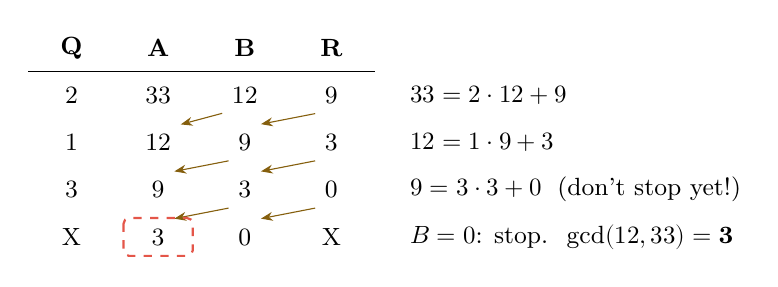
\begin{tikzpicture}[x=11mm,y=6mm]
  \foreach \h [count=\c] in {Q,A,B,R}{\node[font=\small\bfseries] at (\c,0) {\h};}
  \draw (0.5,-0.5) -- (4.5,-0.5);
  \foreach \q/\a/\b/\r [count=\i] in {2/33/12/9, 1/12/9/3, 3/9/3/0, X/3/0/X}{
    \node[font=\small] at (1,-\i) {\q};
    \node[font=\small] (a\i) at (2,-\i) {\a};
    \node[font=\small] (b\i) at (3,-\i) {\b};
    \node[font=\small] (r\i) at (4,-\i) {\r};
  }
  \foreach \i in {1,2,3}{\pgfmathtruncatemacro{\j}{\i+1}
    \draw[-{Stealth[length=1.5mm]},orange!80!black] (b\i.south west) -- (a\j.north east);
    \draw[-{Stealth[length=1.5mm]},orange!80!black] (r\i.south west) -- (b\j.north east);}
  \draw[warn,thick,dashed,rounded corners=2pt] (1.6,-3.6) rectangle (2.4,-4.4);
  \node[font=\small,anchor=west] at (4.8,-1) {$33 = 2\cdot12 + 9$};
  \node[font=\small,anchor=west] at (4.8,-2) {$12 = 1\cdot9 + 3$};
  \node[font=\small,anchor=west] at (4.8,-3) {$9 = 3\cdot3 + 0$ \;(don't stop yet!)};
  \node[font=\small,anchor=west] at (4.8,-4) {$B = 0$: stop. \;$\gcd(12, 33) = \mathbf{3}$};
\end{tikzpicture}
\end{center}

\begin{minipage}[t]{0.48\textwidth}
\centering\small
$\gcd(750, 900)$\\[2pt]
\begin{tabular}{cccc}
\toprule
Q&A&B&R\\
\midrule
1&900&750&150\\
5&750&150&0\\
X&\textbf{150}&0&X\\
\bottomrule
\end{tabular}
\end{minipage}\hfill
\begin{minipage}[t]{0.48\textwidth}
\centering\small
$\gcd(252, 105)$\\[2pt]
\begin{tabular}{cccc}
\toprule
Q&A&B&R\\
\midrule
2&252&105&42\\
2&105&42&21\\
2&42&21&0\\
X&\textbf{21}&0&X\\
\bottomrule
\end{tabular}
\end{minipage}

\medskip
\textbf{Shortcut:} the GCD is the \textbf{last non-zero remainder} (9, 3, \textbf{3} then 0; or 42, \textbf{21} then 0). The extra ``$B = 0$'' row is just where the lecture reads it off.

\subsection{Method 2: recursion}
\begin{center}
\begin{minipage}{0.45\textwidth}
\small\ttfamily
Prerequisite: a > b\\
Euclid\_GCD(a, b):\\
\hspace*{1.5em}if b = 0 then\\
\hspace*{3em}return a;\\
\hspace*{1.5em}else\\
\hspace*{3em}return Euclid\_GCD(b, a mod b);
\end{minipage}
\end{center}
\begin{minipage}[t]{0.42\textwidth}
\small
\textbf{$\gcd(50, 12)$}\\
$= \gcd(12, 50 \bmod 12) = \gcd(12, 2)$\\
$= \gcd(2, 12 \bmod 2) = \gcd(2, 0)$\\
$= \mathbf{2}$
\end{minipage}\hfill
\begin{minipage}[t]{0.55\textwidth}
\small
\textbf{$\gcd(83, 19)$}\\
$= \gcd(19, 7)$ \quad ($83 = 4\cdot19 + 7$)\\
$= \gcd(7, 5)$ \quad ($19 = 2\cdot7 + 5$)\\
$= \gcd(5, 2)$ \quad ($7 = 1\cdot5 + 2$)\\
$= \gcd(2, 1)$ \quad ($5 = 2\cdot2 + 1$)\\
$= \gcd(1, 0) = \mathbf{1}$ \quad ($2 = 2\cdot1 + 0$)
\end{minipage}

\medskip
Both methods do exactly the same divisions; use whichever you like. If you're given $a < b$ (e.g.\ $\gcd(10, 20)$), swap them first.
(The algorithm fixes it on its own anyway: $\gcd(12, 33) \to \gcd(33, 12 \bmod 33) = \gcd(33, 12)$, which wastes one step.)

\subsection{Relatively prime}
\begin{keybox}
$a$ and $b$ are \textbf{relatively prime} (coprime) if $\gcd(a, b) = 1$. Example: 83 and 19.
Coprime numbers need not be prime themselves: $\gcd(8, 9) = 1$.
\end{keybox}
\textbf{Why cryptography cares:}
\begin{itemize}
  \item $a^{-1} \bmod n$ exists \textbf{only if} $\gcd(a, n) = 1$. That was the Hill key condition $\gcd(\det K, 26) = 1$.
  \item The \textbf{extended} Euclidean algorithm (next on the roadmap) runs these same divisions backwards to actually \emph{find} $a^{-1}$, instead of the trial table we used for $23^{-1} \bmod 26$.
  \item RSA key generation picks an $e$ with $\gcd(e, \phi(n)) = 1$.
\end{itemize}
{\small\emph{Not in the lecture:} Euclid is fast because the remainder at least halves every two steps. The slowest inputs are consecutive Fibonacci numbers, e.g.\ $\gcd(89, 55)$ takes 9 divisions, all with quotient 1.}

\textbf{Lecture homework:} $\gcd(1005, 105)$ and $\gcd(529, 123)$. Solutions are in practice Q43.

\begin{examtip}
\begin{itemize}
  \item GCD $=$ HCF. $\gcd(a, b) = \gcd(b, a \bmod b)$, and $\gcd(a, 0) = a$.
  \item Table method: stop when $B = 0$ (not when $R = 0$); the answer is that row's $A$, i.e.\ the last non-zero remainder.
  \item Put the larger number first.
  \item $\gcd = 1$ means relatively prime (coprime), which is exactly when a multiplicative inverse exists.
  \item Show every division as $a = q\cdot b + r$ in exams.
\end{itemize}
\end{examtip}

\begin{fixbox}
\begin{itemize}
  \item All results are correct (checked by script): 3, 25, 1, 3, 150, 21, 2, 1.
  \item Verbal slips only: ``divisors of 13'' means 33 (video 1); ``a = 9'' means 19 (video 2). The slides are right.
  \item Wording: ``$A$ mod $B$'' gives the \emph{remainder}; ``$A$ divided by $B$'' gives the quotient $Q$. The table needs both.
\end{itemize}
\end{fixbox}

% College Lecture 2 (extended Euclid) + Lecture 4 (inverses, Diophantine). All tables generated by script.
\section{Extended Euclidean Algorithm}\label{sec:exteuclid}

Finds $s, t$ with $\boxed{s \cdot a + t \cdot b = \gcd(a, b)}$ along with the gcd.
\begin{keybox}[title=Algorithm (Forouzan table)]
$r_1 = a, r_2 = b$; \; $s_1 = 1, s_2 = 0$; \; $t_1 = 0, t_2 = 1$. While $r_2 > 0$:
\[
q = \lfloor r_1 / r_2 \rfloor,\quad r = r_1 - q r_2,\quad s = s_1 - q s_2,\quad t = t_1 - q t_2;\quad\text{shift } (r_1, r_2) \leftarrow (r_2, r),\ (s_1,s_2) \leftarrow (s_2,s),\ (t_1,t_2) \leftarrow (t_2,t).
\]
At the end: $\gcd = r_1$, \;$s = s_1$, \;$t = t_1$.
\end{keybox}

\textbf{Example}: $a = 161$, $b = 28$.
\begin{center}\small
\begin{tabular}{@{}r|rrr|rrr|rrr@{}}
\toprule
$q$ & $r_1$ & $r_2$ & $r$ & $s_1$ & $s_2$ & $s$ & $t_1$ & $t_2$ & $t$\\
\midrule
5 & 161 & 28 & 21 & 1 & 0 & 1 & 0 & 1 & $-5$\\
1 & 28 & 21 & 7 & 0 & 1 & $-1$ & 1 & $-5$ & 6\\
3 & 21 & 7 & 0 & 1 & $-1$ & 4 & $-5$ & 6 & $-23$\\
 & \textbf{7} & 0 & & $\mathbf{-1}$ & 4 & & \textbf{6} & $-23$ & \\
\bottomrule
\end{tabular}
\end{center}
$\gcd(161, 28) = 7$, $s = -1$, $t = 6$: \;$(-1)(161) + 6(28) = 7$ \checkmark. Other results: $(84, 320) \to \gcd 4$, $s = -19$, $t = 5$; \;$(17, 0) \to 17, 1, 0$; \;$(0, 45) \to 45, 0, 1$.

\subsection{Multiplicative inverse with the table}
To find $b^{-1} \bmod n$: run the table with $r_1 = n$, $r_2 = b$, \textbf{only the $t$ columns} (start $t_1 = 0, t_2 = 1$). If the final $r_1 = 1$, then $b^{-1} = t_1 \bmod n$; if $r_1 \ne 1$, no inverse.
\begin{center}\small
\begin{tabular}{@{}r|rrr|rrr@{}}
\multicolumn{7}{c}{$11^{-1} \bmod 26$}\\
\toprule
$q$ & $r_1$ & $r_2$ & $r$ & $t_1$ & $t_2$ & $t$\\
\midrule
2 & 26 & 11 & 4 & 0 & 1 & $-2$\\
2 & 11 & 4 & 3 & 1 & $-2$ & 5\\
1 & 4 & 3 & 1 & $-2$ & 5 & $-7$\\
3 & 3 & 1 & 0 & 5 & $-7$ & 26\\
 & \textbf{1} & 0 & & $\mathbf{-7}$ & 26 & \\
\bottomrule
\end{tabular}
\quad
\begin{tabular}{@{}r|rrr|rrr@{}}
\multicolumn{7}{c}{$23^{-1} \bmod 100$}\\
\toprule
$q$ & $r_1$ & $r_2$ & $r$ & $t_1$ & $t_2$ & $t$\\
\midrule
4 & 100 & 23 & 8 & 0 & 1 & $-4$\\
2 & 23 & 8 & 7 & 1 & $-4$ & 9\\
1 & 8 & 7 & 1 & $-4$ & 9 & $-13$\\
7 & 7 & 1 & 0 & 9 & $-13$ & 100\\
 & \textbf{1} & 0 & & $\mathbf{-13}$ & 100 & \\
\bottomrule
\end{tabular}
\end{center}
$11^{-1} \equiv -7 \equiv \mathbf{19} \pmod{26}$; \;$23^{-1} \equiv -13 \equiv \mathbf{87} \pmod{100}$; \;$12^{-1} \bmod 26$: final $r_1 = 2$, no inverse.

\subsection{Linear Diophantine equations $ax + by = c$}
Let $d = \gcd(a, b)$. If $d \nmid c$: no solution. If $d \mid c$: infinitely many. Divide by $d$, find $s, t$ with $s(a/d) + t(b/d) = 1$; then
\[
\text{particular: } x_0 = (c/d)\,s,\ \ y_0 = (c/d)\,t \qquad \text{general: } x = x_0 + k\,(b/d),\ \ y = y_0 - k\,(a/d).
\]
\begin{itemize}
  \item $21x + 14y = 35$: $d = 7$; $3x + 2y = 5$, $s = 1$, $t = -1$; particular $(5, -5)$; general $x = 5 + 2k$, $y = -5 - 3k$: $(5,-5), (7,-8), (9,-11), \dots$
  \item Cash a Rs.~100 cheque in Rs.~20 and Rs.~5 notes: $20x + 5y = 100$, $d = 5$, $4x + y = 20$, $s = 0$, $t = 1$; particular $(0, 20)$; non-negative solutions $(0,20), (1,16), (2,12), (3,8), (4,4), (5,0)$.
\end{itemize}

\begin{examtip}
\begin{itemize}
  \item Always show the full table with all columns; the exam awards marks per row.
  \item For an inverse, run with $r_1 = n$ (the modulus) first; a negative $t_1$ is fine, add $n$ at the end.
  \item Check: $s a + t b = \gcd$, or $b \cdot b^{-1} \bmod n = 1$.
\end{itemize}
\end{examtip}

% Videos: relatively prime numbers, Euler's totient (concept), Euler's totient (formulas, solved examples)
\section{Relatively Prime Numbers and Euler's Totient}

\subsection{Relatively prime (co-prime) numbers}
\begin{keybox}
Two numbers are \textbf{relatively prime} if they have no prime factors in common and their only common factor is 1:
\[
\gcd(a, b) = 1 \iff a, b \text{ are relatively prime (co-prime)}
\]
\end{keybox}
\begin{center}\small
\begin{tabular}{@{}lllcl@{}}
\toprule
$a$, $b$ & Divisors & GCD & Co-prime? & Note\\
\midrule
4, 13 & $\{1,2,4\}$, $\{1,13\}$ & 1 & yes & composite + prime\\
15, 21 & $\{1,3,5,15\}$, $\{1,3,7,21\}$ & 3 & \textbf{no} & share the factor 3\\
11, 17 & & 1 & yes & both prime\\
11, 21 & & 1 & yes & prime + composite ($21 = 3\cdot7$)\\
12, 77 & & 1 & yes & \textbf{both composite} ($2^2\cdot3$ and $7\cdot11$)\\
83, 19 & (Euclid: $\gcd(19,7) = \dots = \gcd(1,0)$) & 1 & yes & \\
\bottomrule
\end{tabular}
\end{center}
\textbf{Never judge by looks.} Co-prime numbers can both be composite (12, 77). Always compute the GCD, using Euclid for big numbers.
Lecture homework: $\gcd(790, 121)$ (answer in practice Q48).

\subsection{Euler's totient function $\Phi(n)$}
\begin{keybox}
$\Phi(n)$ = the number of \textbf{positive integers less than $n$} that are \textbf{relatively prime to $n$}.
(Zero and negative numbers don't count.)
\end{keybox}
\textbf{By hand:} check $\gcd(k, n)$ for every $k = 1, \dots, n-1$ and count the 1s.
\begin{center}\small\setlength{\tabcolsep}{5pt}
\begin{tabular}{@{}l*{7}{c}l@{}}
\toprule
$k$ & 1&2&3&4&5&6&7&\\
$\gcd(k, 8)$ & 1&2&1&4&1&2&1&\\
co-prime? & \checkmark&$\times$&\checkmark&$\times$&\checkmark&$\times$&\checkmark& $\Rightarrow \Phi(8) = \mathbf{4}$\\
\bottomrule
\end{tabular}
\end{center}
Similarly $\Phi(5) = 4$ (all of 1--4) and $\Phi(11) = 10$ (all of 1--10). For $n = 1000$ this would take 999 GCDs, hence the formulas.

\subsection{Formulas}
\begin{center}\small
\begin{tabularx}{\textwidth}{@{}l X l@{}}
\toprule
Case & Formula & Example\\
\midrule
1. $n$ is prime & $\Phi(n) = n - 1$ & $\Phi(7) = 6$, $\Phi(31) = 30$\\
2. $n = p \times q$, \textbf{distinct} primes & $\Phi(n) = (p-1)(q-1)$ & $\Phi(21) = 2\cdot6 = 12$\\
3. anything else & $\Phi(n) = n\left(1 - \frac{1}{p_1}\right)\left(1 - \frac{1}{p_2}\right)\cdots$, \;$p_i$ = the \textbf{distinct} primes dividing $n$ & $\Phi(1000) = 400$\\
\bottomrule
\end{tabularx}
\end{center}
The formula in case 3 works for \emph{every} $n$: for a prime, $n(1 - \frac1n) = n - 1$; for $pq$, $pq(1-\frac1p)(1-\frac1q) = (p-1)(q-1)$. Cases 1 and 2 are shortcuts.

\textbf{Example: $\Phi(35)$}, with $35 = 5 \times 7$: $\;(5-1)(7-1) = 4 \times 6 = \mathbf{24}$. Check by crossing out the multiples of 5 and 7 among 1--34:
\begin{center}
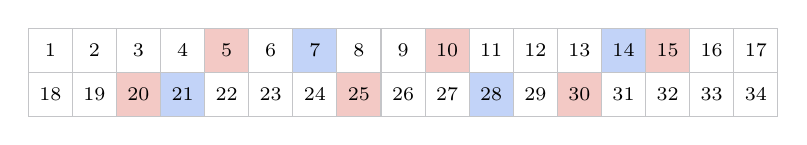
\begin{tikzpicture}[x=5.6mm,y=5.6mm]
  \foreach \k in {1,...,34}{
    \pgfmathtruncatemacro{\col}{mod(\k-1,17)}
    \pgfmathtruncatemacro{\row}{(\k-1)/17}
    \pgfmathtruncatemacro{\mf}{mod(\k,5)}
    \pgfmathtruncatemacro{\ms}{mod(\k,7)}
    \ifnum\mf=0 \fill[warn!30] (\col,-\row) rectangle ++(1,-1);\fi
    \ifnum\ms=0 \fill[acc!30] (\col,-\row) rectangle ++(1,-1);\fi
    \draw[gray!60] (\col,-\row) rectangle ++(1,-1);
    \node[font=\scriptsize] at (\col+0.5,-\row-0.5) {\k};
  }
\end{tikzpicture}\\[2pt]
{\footnotesize red = multiple of 5 (6 numbers), blue = multiple of 7 (4 numbers); $34 - 10 = 24$ white cells}
\end{center}

\begin{keybox}[title=Trap: repeated prime factors]
$25 = 5 \times 5$, but $p$ and $q$ must be \textbf{different}. $(5-1)(5-1) = 16$ is \textbf{wrong}.
Use case 3: $\Phi(25) = 25\left(1 - \frac15\right) = \mathbf{20}$. (Check: of 1--24, only 5, 10, 15, 20 share a factor with 25, so $24 - 4 = 20$.)
\end{keybox}

\textbf{Example: $\Phi(1000)$.} $1000 = 2^3 \cdot 5^3$; the distinct primes are 2 and 5 (\textbf{the exponents don't appear}):
$\;1000 \cdot \frac12 \cdot \frac45 = \mathbf{400}$.

\textbf{Example: $\Phi(7000)$.} $7000 = 2^3 \cdot 5^3 \cdot 7$:
$\;7000 \cdot \frac12 \cdot \frac45 \cdot \frac67 = 7000 \cdot \frac{24}{70} = \mathbf{2400}$.

\textbf{Lecture homework:} $\Phi(369)$ and $\Phi(372)$. Answers in practice Q48.

\subsection{Other useful formulas (mentioned but not shown in the lecture)}
\begin{itemize}
  \item \textbf{Prime power:} $\Phi(p^k) = p^k - p^{k-1}$ (remove the $p^{k-1}$ multiples of $p$). E.g.\ $\Phi(25) = 25 - 5 = 20$, $\Phi(8) = 8 - 4 = 4$.
  \item \textbf{Multiplicative:} $\Phi(mn) = \Phi(m)\,\Phi(n)$ \emph{when $\gcd(m, n) = 1$}. E.g.\ $\Phi(1000) = \Phi(8)\Phi(125) = 4 \cdot 100 = 400$. (If $\gcd \ne 1$ it fails: $\Phi(4) = 2 \ne \Phi(2)\Phi(2) = 1$.)
  \item By convention $\Phi(1) = 1$.
\end{itemize}

\subsection{Why cryptography cares}
\begin{itemize}
  \item $\Phi(n)$ counts the numbers that \textbf{have a multiplicative inverse} mod $n$. $\Phi(26) = 12$: that's exactly the 12 valid Hill determinants (practice Q46).
  \item \textbf{RSA:} $n = p \cdot q$ and $\Phi(n) = (p-1)(q-1)$. The keys satisfy $e \cdot d \equiv 1 \pmod{\Phi(n)}$.
  The bookmarked example: $187 = 11 \cdot 17$, $\Phi(187) = 10 \cdot 16 = 160$, and $7 \cdot 23 = 161 \equiv 1 \pmod{160}$. That's why $88^7 \to 11$ and $11^{23} \to 88$ undo each other.
  \item \textbf{Euler's theorem} (coming next): $a^{\Phi(n)} \equiv 1 \pmod n$ when $\gcd(a, n) = 1$.
\end{itemize}

\begin{examtip}
\begin{itemize}
  \item Co-prime $\iff \gcd = 1$. Neither number has to be prime.
  \item $\Phi(n)$ counts $1 \le k < n$ with $\gcd(k, n) = 1$.
  \item Prime: $n - 1$. Two \textbf{distinct} primes: $(p-1)(q-1)$. Otherwise: $n\prod(1 - 1/p)$ over the \textbf{distinct} primes.
  \item $\Phi(p^2) \ne (p-1)^2$: $\Phi(25) = 20$, not 16.
  \item Always factorise completely first, and ignore the exponents in the product formula.
\end{itemize}
\end{examtip}

\begin{fixbox}
\begin{itemize}
  \item All results correct (checked by script): $\Phi(5) = 4$, $\Phi(11) = 10$, $\Phi(8) = 4$, $\Phi(35) = 24$, $\Phi(25) = 20$, $\Phi(1000) = 400$, $\Phi(7000) = 2400$. Gemini's homework answers ($\Phi(369) = 240$, $\Phi(372) = 120$) are also correct.
  \item The slide's ``case 3'' (``either or both of $a, b$ composite'') makes the product formula look like a last resort. It actually works for all $n$.
  \item ``Less than $n$'' gives $\Phi(1) = 0$, but the standard convention is $\Phi(1) = 1$ (count $1 \le k \le n$). It only matters for $n = 1$.
\end{itemize}
\end{fixbox}

% Videos: Fermat's little theorem, Euler's theorem, primitive roots, multiplicative inverse
\section{Fermat, Euler, Primitive Roots and Inverses}\label{sec:fermat}

\subsection{Fermat's little theorem}
\begin{keybox}
If $p$ is \textbf{prime} and $a$ is a positive integer \textbf{not divisible by $p$}, then
\[
a^{p-1} \equiv 1 \pmod p
\]
\end{keybox}
\textbf{Check both conditions first.} If $p$ isn't prime, or $p \mid a$, the theorem says nothing.
\begin{center}\small
\begin{tabular}{@{}llll@{}}
\toprule
$p$, $a$ & Conditions & Working & Result\\
\midrule
5, 2 & prime, $5 \nmid 2$ & $2^4 = 16 = 3\cdot5 + 1$ & $\equiv 1$ \checkmark\\
13, 11 & prime, $13 \nmid 11$ & $11 \equiv -2$: $(-2)^{12} = \big((-2)^4\big)^3 = 16^3 \equiv 3^3 = 27 \equiv 1$ & $\equiv 1$ \checkmark\\
6, 2 & \textbf{6 not prime} & $2^5 = 32 = 5\cdot6 + 2$ & $\equiv 2 \ne 1$: doesn't apply\\
11, 5 (homework) & prime, $11 \nmid 5$ & $5^2 \equiv 3$, $5^4 \equiv 9 \equiv -2$, $5^8 \equiv 4$, $5^{10} \equiv 4\cdot3 = 12$ & $\equiv 1$ \checkmark\\
\bottomrule
\end{tabular}
\end{center}

\textbf{Three ways the exam uses Fermat}:
\begin{enumerate}[leftmargin=1.5em]
  \item \textbf{Shrink a huge exponent}: $a^b \equiv a^{\,b \bmod (p-1)} \pmod p$ (when $p \nmid a$).
  E.g.\ $145^{102} \bmod 101$: $102 \bmod 100 = 2$, so $44^2 \equiv 17$ (2024--25 paper, Q5).
  \item \textbf{Find an inverse}: $a^{-1} \equiv a^{p-2} \pmod p$, because $a \cdot a^{p-2} = a^{p-1} \equiv 1$. E.g.\ $2^{-1} \bmod 13 = 2^{11} \bmod 13 = 7$ (check $2\cdot7 = 14 \equiv 1$).
  \item \textbf{Second form}, true for \emph{every} $a$: $a^p \equiv a \pmod p$. E.g.\ $658^{17} \equiv 658 \equiv 12 \pmod{17}$ (same paper).
\end{enumerate}
\textbf{Fermat as a primality test, and its trap:} if $a^{n-1} \not\equiv 1 \pmod n$, then $n$ is \textbf{definitely composite} (e.g.\ $2^{14} \bmod 15 = 4$). But $a^{n-1} \equiv 1$ does \textbf{not} prove $n$ prime: $2^{340} \equiv 1 \pmod{341}$, yet $341 = 11\cdot31$.

\subsection{Euler's theorem}
\begin{keybox}
For positive integers $a$ and $n$ that are \textbf{relatively prime} ($\gcd(a, n) = 1$):
\[
a^{\Phi(n)} \equiv 1 \pmod n
\]
$n$ need not be prime. When $n = p$ is prime, $\Phi(p) = p - 1$ and this \textbf{is} Fermat's theorem.
\end{keybox}
\begin{center}\small
\begin{tabular}{@{}llll@{}}
\toprule
$a$, $n$ & $\gcd$ & Working & Result\\
\midrule
3, 10 & 1 & $\Phi(10) = 4$; $3^4 = 81 = 8\cdot10 + 1$ & $\equiv 1$ \checkmark\\
2, 10 & \textbf{2} & $2^4 = 16 \equiv 6$ & $\ne 1$: doesn't apply\\
10, 11 & 1 & $\Phi(11) = 10$; $10 \equiv -1$, $(-1)^{10} = 1$ & $\equiv 1$ \checkmark\\
11, 33 (homework) & \textbf{11} & $\Phi(33) = 20$; $11^k \bmod 33$ alternates $11, 22, 11, 22, \dots$ & $11^{20} \equiv 22 \ne 1$\\
\bottomrule
\end{tabular}
\end{center}
In the homework, every power of 11 is a multiple of 11, so it can never be $\equiv 1 \pmod{33}$. That's \emph{why} $\gcd = 1$ is required.

\textbf{The same three tools, for any $n$} (with $\gcd(a, n) = 1$):
\begin{itemize}
  \item Exponent reduction: $a^b \equiv a^{\,b \bmod \Phi(n)} \pmod n$. E.g.\ $11^{2024} \bmod 35$: $\Phi(35) = 24$, $2024 \bmod 24 = 8$, so $11^8 \equiv 16$.
  \item Inverse: $a^{-1} \equiv a^{\Phi(n) - 1} \pmod n$. E.g.\ $7^{-1} \bmod 15 = 7^7 \bmod 15 = 13$ ($7 \cdot 13 = 91 = 6\cdot15 + 1$).
  \item RSA works because of Euler: $e\cdot d \equiv 1 \pmod{\Phi(n)}$ gives $M^{ed} = M^{1 + k\Phi(n)} \equiv M \pmod n$.
\end{itemize}

\subsection{Primitive roots}
Needed for \textbf{Diffie--Hellman key exchange}.
\begin{keybox}
$\alpha$ is a \textbf{primitive root} of the prime $p$ if $\;\alpha^1, \alpha^2, \dots, \alpha^{p-1} \pmod p\;$ are all \textbf{distinct}, i.e.\ they produce every number $1, \dots, p-1$ exactly once.
(General form: every number co-prime to $n$ is a power of $\alpha$ mod $n$.)
\end{keybox}
\begin{center}\small
\begin{tabular}{@{}lll@{}}
\toprule
Test & Powers $\alpha^1, \alpha^2, \dots$ (mod $p$) & Verdict\\
\midrule
2 mod 5 & 2, 4, 3, 1 & all distinct: \textbf{yes}\\
3 mod 7 & 3, 2, 6, 4, 5, 1 & \textbf{yes}\\
2 mod 7 & 2, 4, \textbf{1}, 2, 4, 1 & 1 at step 3, repeats: \textbf{no}\\
2 mod 11 (homework) & 2, 4, 8, 5, 10, 9, 7, 3, 6, 1 & \textbf{yes}\\
\bottomrule
\end{tabular}
\end{center}
\textbf{Chain trick:} get each power from the previous one ($3^4 \equiv 6 \times 3 = 18 \equiv 4$); never compute $3^6 = 729$.
\textbf{Early stop:} once you reach 1 (or any repeat) before $\alpha^{p-1}$, the powers start cycling, so it's not a primitive root.

\textbf{Homework, primitive roots of 5:} 1 never works ($1^k = 1$). 2 works (above). $3$: 3, 4, 2, 1, so yes. $4$: 4, 1, 4, 1, so no. Answer: \textbf{2 and 3}.

\subsubsection*{Going further (not in the lecture, but standard and useful)}
\begin{itemize}
  \item The \textbf{order} of $a$ mod $p$ is the smallest $k$ with $a^k \equiv 1$. A primitive root has order $p - 1$ (the maximum).
  Mod 7 the orders are: 1$\to$1, 2$\to$3, \textbf{3$\to$6}, 4$\to$3, \textbf{5$\to$6}, 6$\to$2. The order always divides $p - 1$.
  \item A prime $p$ has exactly $\boldsymbol{\Phi(p-1)}$ primitive roots: 5 has $\Phi(4) = 2$ (2, 3); 7 has 2 (3, 5); 11 has 4 (2, 6, 7, 8); 13 has 4 (2, 6, 7, 11).
  \item \textbf{Fast test:} $\alpha$ is a primitive root of $p$ $\iff$ $\alpha^{(p-1)/q} \not\equiv 1$ for every prime $q \mid (p-1)$. E.g.\ 3 mod 17: $16 = 2^4$, so check only $3^8 \bmod 17 = 16 \ne 1$, and 3 \textbf{is} a primitive root.
  \item Not every modulus has one: $\mathbb{Z}_8^* = \{1, 3, 5, 7\}$ has every order $\le 2$ but $\Phi(8) = 4$, so \textbf{none}. (Primitive roots exist only for $n = 2, 4, p^k, 2p^k$.)
\end{itemize}

\subsection{Multiplicative inverse mod $n$}
\begin{keybox}
$A^{-1}$ is the multiplicative inverse of $A$ mod $n$ if $\;A \times A^{-1} \equiv 1 \pmod n$.
It \textbf{exists if and only if $\gcd(A, n) = 1$}, and it \textbf{depends on $n$}.
\end{keybox}
\begin{center}\small
\begin{tabular}{@{}lllll@{}}
\toprule
$A \bmod n$ & $\gcd$ & Search & Inverse & Note\\
\midrule
$3 \bmod 5$ & 1 & $3\cdot2 = 6 \equiv 1$ & \textbf{2} & so $2^{-1} \bmod 5 = 3$ too\\
$2 \bmod 11$ & 1 & $2\cdot6 = 12 \equiv 1$ & \textbf{6} & \\
$4 \bmod 5$ & 1 & $4\cdot4 = 16 \equiv 1$ & \textbf{4} & its own inverse ($4 \equiv -1$)\\
$2 \bmod 7$ & 1 & $2\cdot4 = 8 \equiv 1$ & \textbf{4} & not 3: depends on $n$!\\
$5 \bmod 10$ & \textbf{5} & $5k \bmod 10 \in \{0, 5\}$ only & \textbf{none} & \\
\bottomrule
\end{tabular}
\end{center}
\textbf{Which method?}
\begin{center}\small
\begin{tabularx}{\textwidth}{@{}l X@{}}
\toprule
Trial ($A\cdot1, A\cdot2, \dots$) & small $n$ only\\
Fermat: $A^{p-2} \bmod p$ & $n$ prime (use repeated squaring)\\
Euler: $A^{\Phi(n)-1} \bmod n$ & you know $\Phi(n)$; e.g.\ $8^{-1} \bmod 77 = 8^{59} \bmod 77 = 29$\\
\textbf{Extended Euclid} & the general method; also detects ``no inverse''. \textbf{This is what the exam asks} (Section~\ref{sec:pastpapers} method box; 2024--25 Q7)\\
\bottomrule
\end{tabularx}
\end{center}

\begin{examtip}
\begin{itemize}
  \item Fermat: $p$ prime and $p \nmid a$. Euler: $\gcd(a, n) = 1$. State the conditions before using either.
  \item Reduce exponents mod $p - 1$ (Fermat) or mod $\Phi(n)$ (Euler), \emph{never} mod $p$ or $n$.
  \item $a^{-1} \equiv a^{p-2} \pmod p$ and $a^{-1} \equiv a^{\Phi(n)-1} \pmod n$.
  \item Primitive root table: chain-multiply by $\alpha$, stop at the first repeat. Count $= \Phi(p-1)$.
  \item $a^{n-1} \not\equiv 1$ proves $n$ composite; $a^{n-1} \equiv 1$ proves nothing (341).
\end{itemize}
\end{examtip}

\begin{fixbox}
\begin{itemize}
  \item All results checked by script; Gemini's homework answers are correct ($5^{10} \equiv 1 \pmod{11}$; $11^{20} \equiv 22 \pmod{33}$; 2 is a primitive root of 11; the primitive roots of 5 are 2 and 3).
  \item Slide notation: ``$-2^{12}$'' and ``$-1^{10}$'' mean $(-2)^{12}$ and $(-1)^{10}$. Without brackets, $-2^{12} = -(2^{12})$. Write the brackets in exams.
  \item The general definition of a primitive root (for any $n$) was given but not explained. Only $n = 2, 4, p^k, 2p^k$ have primitive roots ($\mathbb{Z}_8^*$ has none).
\end{itemize}
\end{fixbox}

% College Lectures 10-11: primes, primality tests, Fermat/Euler (second versions), factorization, CRT, exponentiation, discrete logs. All numbers verified by script.
\section{Primes, Primality Tests, CRT and Discrete Logs}

\subsection{Counting and checking primes}
\begin{itemize}
  \item Infinitely many primes. $\pi(n)$ $=$ number of primes $\le n$: $\pi(10) = 4$, $\pi(20) = 8$, $\pi(50) = 15$, $\pi(100) = 25$. Bounds (Gauss, Lagrange): $\dfrac{n}{\ln n} < \pi(n) < \dfrac{n}{\ln n - 1.08366}$; for $n = 10^6$: $72{,}382 < \pi(n) < 78{,}543$ (actual 78{,}498).
  \item \textbf{Is $n$ prime?} Test divisibility by every prime $\le \lfloor\sqrt n\rfloor$. $97$: $\lfloor\sqrt{97}\rfloor = 9$, none of 2, 3, 5, 7 divide $\Rightarrow$ prime. $301$: check primes $\le 17$; $7 \mid 301$ ($= 7 \times 43$) $\Rightarrow$ composite.
  \item \textbf{Mersenne} $M_p = 2^p - 1$: prime for $p = 2, 3, 5, 7, 13, 17$ but $M_{11} = 2047 = 23 \times 89$. \textbf{Fermat} $F_n = 2^{2^n} + 1$: $F_0..F_4 = 3, 5, 17, 257, 65537$ are prime; $F_5 = 4294967297 = 641 \times 6700417$.
\end{itemize}

\subsection{Fermat and Euler: second versions and inverses}
\begin{center}\small
\begin{tabular}{@{}lll@{}}
\toprule
 & First version & Second version (no coprime condition)\\
\midrule
Fermat ($p$ prime) & $a^{p-1} \equiv 1 \pmod p$ if $p \nmid a$ & $a^p \equiv a \pmod p$\\
Euler & $a^{\phi(n)} \equiv 1 \pmod n$ if $\gcd(a,n) = 1$ & $a^{k\phi(n)+1} \equiv a \pmod n$ (for $n = pq$)\\
\bottomrule
\end{tabular}
\end{center}
\textbf{Inverses without extended Euclid}: $a^{-1} \equiv a^{p-2} \pmod p$; \;$a^{-1} \equiv a^{\phi(n)-1} \pmod n$.
\begin{center}\small
\begin{tabular}{@{}ll@{\qquad}ll@{}}
\toprule
$8^{-1} \bmod 17 = 8^{15}$ & $= 15$ & $8^{-1} \bmod 77 = 8^{59}$ & $= 29$ \;($\phi = 60$)\\
$5^{-1} \bmod 23 = 5^{21}$ & $= 14$ & $7^{-1} \bmod 15 = 7^{7}$ & $= 13$ \;($\phi = 8$)\\
$60^{-1} \bmod 101 = 60^{99}$ & $= 32$ & $60^{-1} \bmod 187 = 60^{159}$ & $= 53$ \;($\phi = 160$)\\
$22^{-1} \bmod 211 = 22^{209}$ & $= 48$ & $71^{-1} \bmod 100 = 71^{39}$ & $= 31$ \;($\phi = 40$)\\
\bottomrule
\end{tabular}
\end{center}
Examples: $6^{10} \bmod 11 = 1$; \;$3^{12} \bmod 11 = 3^{11} \cdot 3 \equiv 3 \cdot 3 = 9$; \;$6^{24} \bmod 35 = 1$ ($\phi(35) = 24$); \;$20^{62} \bmod 77 = 20^{60+1} \cdot 20 \equiv 20 \cdot 20 = 400 \equiv \mathbf{15}$.

$\phi$ refresher: $\phi(240) = \phi(2^4)\phi(3)\phi(5) = 8 \cdot 2 \cdot 4 = 64$; \;$\phi(49) = 7^2 - 7 = 42$ (\textbf{not} $\phi(7)^2 = 36$: 7 and 7 aren't coprime); $|\mathbb{Z}_{14}^*| = \phi(14) = 6$: $\{1, 3, 5, 9, 11, 13\}$. For $n > 2$, $\phi(n)$ is even.

\subsection{Primality testing}
\textbf{Deterministic}: divisibility test (exponential: $2^{n/2}$ bit operations for an $n$-bit number), AKS (polynomial, $O((\log_2 n)^{12})$). \textbf{Probabilistic}: fast, may wrongly say ``prime''.
\begin{itemize}
  \item \textbf{Fermat test}: if $a^{n-1} \not\equiv 1 \pmod n$, $n$ is composite; if $\equiv 1$, ``probably prime''. Fooled by \textbf{Carmichael numbers}: $2^{560} \equiv 1 \pmod{561}$ but $561 = 3 \cdot 11 \cdot 17$.
  \item \textbf{Square-root test}: if $n$ is prime, the only square roots of 1 mod $n$ are $\pm1$. Mod 7: $\{1, 6\}$; mod 17: $\{1, 16\}$; mod 8: $\{1, 3, 5, 7\}$ (composite); mod 22: only $\{1, 21\}$ even though 22 is composite, so the test is one-way.
\end{itemize}
\begin{keybox}[title=Miller--Rabin test (base $a$)]
Write $n - 1 = m \cdot 2^k$ with $m$ odd. $T = a^m \bmod n$. If $T = \pm1$: \textbf{prime}. Then repeat up to $k - 1$ times: $T \leftarrow T^2 \bmod n$; if $T = +1$: \textbf{composite}; if $T = -1$: \textbf{prime}. If the loop ends: \textbf{composite}.
\end{keybox}
\begin{center}\small
\begin{tabular}{@{}llll@{}}
\toprule
$n$, base & $n - 1 = m \cdot 2^k$ & $T$ sequence & Result\\
\midrule
561, 2 & $35 \cdot 2^4$ & 263, 166, 67, \textbf{1} & composite (correct: Carmichael caught)\\
27, 2 & $13 \cdot 2^1$ & 11 (no loop since $k - 1 = 0$) & composite\\
61, 2 & $15 \cdot 2^2$ & 11, \textbf{60} ($= -1$) & prime\\
4033, 2 & $63 \cdot 2^6$ & 3521, \textbf{4032} ($= -1$) & ``prime'' (wrong: $4033 = 37 \times 109$)\\
4033, 3 & $63 \cdot 2^6$ & 3551, 2443, 3442, 2443, 3442, 2443 & composite\\
\bottomrule
\end{tabular}
\end{center}
\textbf{Recommended practice}: divisibility test by small primes first, then Miller--Rabin with several bases (4033 fools base 2 but not base 3).

\subsection{Factorization}
\textbf{Fundamental theorem}: $n = p_1^{e_1} \cdots p_k^{e_k}$ uniquely. $\gcd = \prod p_i^{\min(a_i, b_i)}$, \;$\operatorname{lcm} = \prod p_i^{\max(a_i, b_i)}$, \;$\gcd \times \operatorname{lcm} = a \times b$.
\begin{itemize}
  \item \textbf{Trial division}: divide by $a = 2, 3, \dots \le \sqrt n$, repeatedly. $1233 = 3^2 \times 137$; $1523357784 = 2^3 \times 3^2 \times 13 \times 37 \times 43987$.
  \item \textbf{Fermat's method}: find $x$ with $x^2 - n = y^2$; then $n = (x + y)(x - y)$. Start $x = \lceil\sqrt n\rceil$ and step up. $n = 5959$: $x = 78$, $w = 125$; $79$: $282$; $80$: $441 = 21^2$ $\Rightarrow 5959 = 101 \times 59$. Fast when the factors are close (for $4033$ it takes 10 steps: $73^2 - 4033 = 36^2$, so $109 \times 37$).
  \item Others (named on slides): Pollard $p - 1$, Pollard rho, quadratic sieve, number field sieve.
\end{itemize}

\subsection{Chinese remainder theorem}
Solves $x \equiv a_1 \pmod{m_1}, \dots, x \equiv a_k \pmod{m_k}$ with \textbf{pairwise coprime} moduli; the solution is unique mod $M$.
\begin{keybox}[title=Four steps]
1.\ $M = m_1 m_2 \cdots m_k$. \;2.\ $M_i = M / m_i$. \;3.\ $M_i^{-1} \bmod m_i$. \;4.\ $x = \left(\sum a_i M_i M_i^{-1}\right) \bmod M$.
\end{keybox}
\begin{center}\small
\begin{tabular}{@{}lllll@{}}
\toprule
System & $M$ & $M_i$ & $M_i^{-1}$ & $x$\\
\midrule
$x \equiv 2 \ (3),\ 3\ (5),\ 2\ (7)$ & 105 & 35, 21, 15 & 2, 1, 1 & $(140 + 63 + 30) \bmod 105 = \mathbf{23}$\\
$x \equiv 3\ (7),\ 3\ (13),\ 0\ (12)$ & 1092 & 156, 84, 91 & 4, 11, 7 & \textbf{276}\\
$S \equiv 1\ (11),\ 12\ (13),\ 2\ (17)$ & 2431 & 221, 187, 143 & 1, 8, 5 & \textbf{155}\\
\bottomrule
\end{tabular}
\end{center}
\textbf{Uses}: secret sharing (the third row: any 3 of the 4 shares $\{1, 12, 2, 3\}$ mod $\{11, 13, 17, 19\}$ recover $S = 155$); arithmetic on big numbers with small moduli: $123 + 334$ via residues mod 99, 98, 97 gives $z \equiv 61, 65, 69$ $\Rightarrow z = 457$; RSA decryption speed-up.

\subsection{Fast exponentiation (square-and-multiply)}
Scan the exponent bits from the least significant: multiply $y$ by the current $a$ when the bit is 1; square $a$ every step. $17^{22} \bmod 21$, $22 = 10110_2$:
\begin{center}\small
\begin{tabular}{@{}ccll@{}}
\toprule
$i$ & $x_i$ & Multiply ($y$, start 1) & Square ($a$, start 17)\\
\midrule
0 & 0 & -- & $a = 17^2 \bmod 21 = 16$\\
1 & 1 & $y = 1 \cdot 16 = 16$ & $a = 16^2 \bmod 21 = 4$\\
2 & 1 & $y = 16 \cdot 4 \bmod 21 = 1$ & $a = 16$\\
3 & 0 & -- & $a = 4$\\
4 & 1 & $y = 1 \cdot 4 = \mathbf{4}$ & (not needed)\\
\bottomrule
\end{tabular}
\end{center}
Cost: about $\log_2 x$ squarings, versus $x$ multiplications naively. (Section~\ref{sec:modexp} has the left-to-right version used in the Neso videos.)

\subsection{Order, primitive roots, discrete logarithms}
\begin{itemize}
  \item \textbf{Order of the group} $|\mathbb{Z}_n^*| = \phi(n)$; e.g.\ $|\mathbb{Z}_{21}^*| = 12$: $\{1, 2, 4, 5, 8, 10, 11, 13, 16, 17, 19, 20\}$.
  \item \textbf{Order of an element} $\operatorname{ord}(a)$: smallest $i$ with $a^i \equiv 1$; it \textbf{divides} $\phi(n)$ (Lagrange). In $\mathbb{Z}_{10}^*$: $\operatorname{ord}(1, 3, 7, 9) = 1, 4, 4, 2$. In $\mathbb{Z}_8^*$: all non-identity elements have order 2, so \textbf{no primitive root}.
  \item \textbf{Primitive root}: $\operatorname{ord}(a) = \phi(n)$. Exist only for $n = 2, 4, p^t, 2p^t$; if they exist there are $\phi(\phi(n))$ of them. $\mathbb{Z}_7^*$: orders $1, 3, 6, 3, 6, 2$ for $a = 1..6$; primitive roots \textbf{3 and 5} ($\phi(6) = 2$ \checkmark).
  \item \textbf{Discrete log}: if $g$ is a primitive root of $p$, every $y \in \mathbb{Z}_p^*$ is $g^x$ for a unique $x \in [1, p-1]$; $x = L_g\, y$. Easy one way (fast exponentiation), believed hard the other way (exhaustive search) $\Rightarrow$ basis of Diffie--Hellman and ElGamal.
\end{itemize}
\begin{center}\small
\begin{tabular}{@{}c|cccccc@{}}
$y$ & 1&2&3&4&5&6\\ \midrule
$L_3 y$ (mod 7) & 6&2&1&4&5&3\\
$L_5 y$ (mod 7) & 6&4&5&2&1&3\\
\end{tabular}
\qquad
\begin{minipage}{0.45\textwidth}\small
$4 \equiv 3^x \pmod 7 \Rightarrow x = L_3 4 = 4$.\\
$6 \equiv 5^x \pmod 7 \Rightarrow x = L_5 6 = 3$.\\
Rules (mod $\phi(n)$): $L_g 1 = 0$, \;$L_g(xy) = L_g x + L_g y$, \;$L_g x^k = k L_g x$.
\end{minipage}
\end{center}

\begin{fixbox}
\begin{itemize}
  \item Slide: ``561 = 33 $\times$ 17'' is true but not the factorisation into primes: $561 = 3 \times 11 \times 17$ (a Carmichael number).
  \item Slide's $\phi(1) = 0$ (Forouzan's convention for ``integers smaller than $n$''); the standard convention is $\phi(1) = 1$. It never matters in RSA.
  \item Euler's second version $a^{k\phi(n)+1} \equiv a$ holds for squarefree $n$ (like $n = pq$ in RSA), not every $n$; e.g.\ it fails for $n = 4$, $a = 2$.
\end{itemize}
\end{fixbox}

% College Lecture 6: groups, rings, fields, GF(p), GF(2^n). All polynomial results verified by script.
\section{Algebraic Structures: Groups, Rings, Fields}\label{sec:algebra}

\subsection{Groups}
A \textbf{group} $G = \langle S, \bullet \rangle$: a set with one operation satisfying
\textbf{closure}, \textbf{associativity}, \textbf{identity} $e$ ($a \bullet e = e \bullet a = a$), \textbf{inverse} ($a \bullet a' = e$). Add \textbf{commutativity} $\Rightarrow$ \textbf{abelian} (commutative) group.
\begin{itemize}
  \item $\langle \mathbb{Z}_n, + \rangle$: abelian, identity 0, inverse of $a$ is $n - a$ (so subtraction works).
  \item $\langle \mathbb{Z}_n^*, \times \rangle$: abelian, identity 1, inverses via extended Euclid (so division works).
  \item \textbf{Permutation group} (all 6 permutations of 3 elements under composition): a group but \textbf{not abelian}. Closure means two successive permutations equal one permutation, so \textbf{applying two transposition ciphers in a row is no stronger than one}.
  \item From an operation table: the identity is the element whose row copies the header; the inverse of $a$ is wherever the identity appears in $a$'s row. (Slide table on $\{a,b,c,d\}$: identity $a$, inverse pairs $(a,a), (b,d), (c,c)$.)
\end{itemize}
\textbf{Finite group}, \textbf{order} $|G|$ (number of elements). \textbf{Subgroup}: a subset that is a group under the \emph{same} operation. ($\langle \mathbb{Z}_{10}, + \rangle$ is \textbf{not} a subgroup of $\langle \mathbb{Z}_{12}, + \rangle$: the operations differ, mod 10 vs mod 12.)

\textbf{Cyclic subgroup} generated by $a$: $\{a^0, a^1, a^2, \dots\}$ (powers mean repeated application of the operation). \textbf{Cyclic group}: generated by one element, called a \textbf{generator}.
\begin{center}\small
\begin{tabular}{@{}lll@{}}
\toprule
Group & Cyclic subgroups & Generators\\
\midrule
$\langle \mathbb{Z}_6, + \rangle$ & $\{0\}$, $\{0, 2, 4\}$ (from 2, 4), $\{0, 3\}$, all of $\mathbb{Z}_6$ (from 1, 5) & 1, 5\\
$\langle \mathbb{Z}_{10}^*, \times \rangle = \{1, 3, 7, 9\}$ & $\{1\}$, $\{1, 9\}$, all of $G$ (from 3, 7) & 3, 7\\
\bottomrule
\end{tabular}
\end{center}
\textbf{Lagrange}: $|H|$ divides $|G|$. \textbf{Order of an element} $=$ order of the cyclic subgroup it generates: in $\mathbb{Z}_6$, ord$(0..5) = 1, 6, 3, 2, 3, 6$; in $\mathbb{Z}_{10}^*$, ord$(1, 3, 7, 9) = 1, 4, 4, 2$.

\subsection{Rings and fields}
\begin{center}\small
\begin{tabularx}{\textwidth}{@{}l X X l@{}}
\toprule
Structure & First operation ($+$) & Second operation ($\times$) & Example\\
\midrule
Group & all 4 (5 if abelian) & -- & $\mathbb{Z}_n$, $\mathbb{Z}_n^*$\\
Ring & all 5 & closure, associativity (+ commutativity: commutative ring); distributes over $+$ & $\langle \mathbb{Z}, +, \times \rangle$\\
Field & all 5 & all 5, except 0 has no multiplicative inverse & $\mathbb{Z}_p$, GF$(2^n)$\\
\bottomrule
\end{tabularx}
\end{center}
$\langle \mathbb{Z}, +, \times\rangle$ is a commutative ring, not a field: $12 / 5 = 2.4 \notin \mathbb{Z}$. A field supports $+, -, \times, \div$ (except $\div 0$).

\subsection{Finite fields}
\begin{keybox}
\textbf{Galois}: a finite field must have $p^n$ elements ($p$ prime, $n \ge 1$): GF$(p^n)$. For $n = 1$, GF$(p) = \mathbb{Z}_p$ with $+$ and $\times$ mod $p$.
\end{keybox}
\textbf{GF(2)} $= \{0, 1\}$: addition $=$ subtraction $=$ \textbf{XOR}, multiplication $=$ \textbf{AND}. \textbf{GF(5)}: multiplicative inverses $1 \leftrightarrow 1$, $2 \leftrightarrow 3$, $4 \leftrightarrow 4$; additive inverses $(1,4), (2,3)$.

\textbf{Why GF$(2^n)$?} Computers store $n$-bit words ($0..2^n - 1$), but $2^n$ isn't prime, so $\mathbb{Z}_{2^n}$ isn't a field. Using the largest prime below $2^n$ wastes values (for $n = 8$: 251 is the largest prime, so 251--255 are unusable). GF$(2^n)$ uses \emph{all} $n$-bit words.

\subsection{GF$(2^n)$ arithmetic}
An $n$-bit word is a polynomial of degree $\le n - 1$ with coefficients in GF(2): \ttx{10011001} $= x^7 + x^4 + x^3 + 1$; \;$x^5 + x^2 + x \to$ \ttx{00100110}.
\begin{itemize}
  \item \textbf{Addition $=$ subtraction $=$ XOR} of the bit strings (no reduction needed): $(x^5 + x^2 + x) + (x^3 + x^2 + 1)$ $=$ \ttx{00100110} $\oplus$ \ttx{00001101} $=$ \ttx{00101011} $= x^5 + x^3 + x + 1$.
  \item \textbf{Multiplication}: multiply normally (coefficients mod 2), then reduce modulo an \textbf{irreducible polynomial} of degree $n$ (cannot be factored into lower-degree polynomials; plays the role of a prime). AES uses $m(x) = x^8 + x^4 + x^3 + x + 1$ (\ttx{0x11B}).
\end{itemize}
Irreducible polynomials: degree 1: $x$, $x + 1$; degree 2: $x^2 + x + 1$; degree 3: $x^3 + x + 1$, $x^3 + x^2 + 1$; degree 4: $x^4 + x + 1$, $x^4 + x^3 + 1$, $x^4 + x^3 + x^2 + x + 1$.

\begin{keybox}[title={Worked: $(x^5 + x^2 + x) \otimes (x^7 + x^4 + x^3 + x^2 + x)$ in GF$(2^8)$}]
Product: $x^{12} + x^9 + x^8 + x^7 + x^6 + \dots$; after cancelling pairs, $x^{12} + x^7 + x^2$.\\
Divide by $x^8 + x^4 + x^3 + x + 1$: quotient $x^4 + 1$, \textbf{remainder $x^5 + x^3 + x^2 + x + 1$} (the answer).\\
\textbf{Shortcut} (repeated multiply-by-$x$): $x \cdot f$ is a left shift; if a bit falls off the top (degree 8), XOR with \ttx{00011011}. With $P_2 = x^7 + x^4 + x^3 + x^2 + x$:
\begin{center}\small
\begin{tabular}{@{}lll@{}}
$x^0 P_2$ & $x^7 + x^4 + x^3 + x^2 + x$ & \\
$x^1 P_2$ & $x^5 + x^2 + x + 1$ & reduced\\
$x^2 P_2$ & $x^6 + x^3 + x^2 + x$ & \\
$x^3 P_2$ & $x^7 + x^4 + x^3 + x^2$ & \\
$x^4 P_2$ & $x^5 + x + 1$ & reduced\\
$x^5 P_2$ & $x^6 + x^2 + x$ & \\
\end{tabular}
\end{center}
$P_1 \otimes P_2 = x^5P_2 + x^2P_2 + xP_2 = (x^6 + x^2 + x) + (x^6 + x^3 + x^2 + x) + (x^5 + x^2 + x + 1) = x^5 + x^3 + x^2 + x + 1$ \checkmark.
\end{keybox}

\textbf{Inverses}: extended Euclid on polynomials (subtraction $=$ XOR), $r_1 = m(x)$, $r_2 = a(x)$, track $t$.
\begin{center}\small
\begin{tabular}{@{}llllll@{}}
\multicolumn{6}{c}{$(x^2 + 1)^{-1}$ in GF$(2^4)$ mod $x^4 + x + 1$}\\
\toprule
$q$ & $r_1$ & $r_2$ & $r$ & $t_1$, $t_2$ & $t$\\
\midrule
$x^2 + 1$ & $x^4 + x + 1$ & $x^2 + 1$ & $x$ & $0$, $1$ & $x^2 + 1$\\
$x$ & $x^2 + 1$ & $x$ & $1$ & $1$, $x^2 + 1$ & $x^3 + x + 1$\\
$x$ & $x$ & $1$ & $0$ & $x^2 + 1$, $x^3 + x + 1$ & \\
\bottomrule
\end{tabular}
\end{center}
$\Rightarrow (x^2 + 1)^{-1} = \mathbf{x^3 + x + 1}$. Likewise $(x^5)^{-1} = x^5 + x^4 + x^3 + x$ in GF$(2^8)$ (4 rows; quotients $x^3$, $x + 1$, $x$, $x^3 + x^2 + 1$).

\textbf{GF$(2^2)$} with modulus $x^2 + x + 1$ (elements 00, 01, 10, 11 $= 0, 1, x, x+1$): $x \cdot x = x + 1$, \;$x(x + 1) = 1$, \;$(x+1)^2 = x$. GF$(2^3)$ uses $x^3 + x^2 + 1$ on the slides.

\begin{examtip}
\begin{itemize}
  \item Define group/ring/field by listing the properties per operation; give $\mathbb{Z}_n$, $\mathbb{Z}$, $\mathbb{Z}_p$ as the examples.
  \item In GF$(2^n)$: add with XOR; multiply then reduce; check degree $< n$; the past papers ask for an inverse with the full extended-Euclid table (Section~\ref{sec:pastpapers}).
\end{itemize}
\end{examtip}

\begin{fixbox}
\begin{itemize}
  \item Slide: a field's second operation ``satisfies all five properties \dots\ except that the identity of the first operation has no inverse''. Read as: every element except 0 has a multiplicative inverse.
\end{itemize}
\end{fixbox}

% College Lecture 7: modern symmetric-key ciphers
\section{Modern Symmetric-Key Ciphers}

Traditional ciphers are character-oriented; modern ones are \textbf{bit-oriented} (text, numbers, images, audio all become bits). A \textbf{modern block cipher} encrypts an $n$-bit block with a $k$-bit key; decryption must be the inverse.

\textbf{Padding}: 100 characters of 8-bit ASCII $= 800$ bits; blocks of 64: $|Pad| = -800 \bmod 64 = 32$ bits $\Rightarrow$ 832 bits $=$ 13 blocks (only the last is padded).

\begin{keybox}[title=Diffusion vs.\ confusion (Shannon)]
\textbf{Diffusion} hides the relation between \textbf{ciphertext and plaintext}: changing one plaintext bit changes many ciphertext bits (defeats ciphertext statistics).\\
\textbf{Confusion} hides the relation between \textbf{ciphertext and key}: changing one key bit changes most ciphertext bits (stops recovering the key).\\
P-boxes give diffusion; S-boxes give confusion.
\end{keybox}

\subsection{Components}
\textbf{P-box} (permutation box, bit transposition):
\begin{center}\small
\begin{tabular}{@{}llll@{}}
\toprule
Type & In/out & Table entries & Invertible?\\
\midrule
Straight & $n \to n$ & a permutation of $1..n$ ($n!$ possible) & \textbf{yes}\\
Expansion & $n \to m$, $m > n$ & $m$ entries, some inputs repeated & no\\
Compression & $n \to m$, $m < n$ & $m$ entries, some inputs missing (blocked) & no\\
\bottomrule
\end{tabular}
\end{center}
Example: an $8 \times 8$ straight P-box moving the middle bits 4, 5 to the ends without disturbing the others: table \ttx{[4 1 2 3 6 7 8 5]} (output position $i$ takes input bit table[$i$]). Slides' $12 \times 16$ expansion table repeats inputs 1, 3, 9, 12; the $32 \times 24$ compression table blocks inputs 7, 8, 9, 15, 16, 23, 24, 25.

\textbf{S-box}: a small substitution, $n$ input bits to $m$ output bits ($m$, $n$ may differ). \textbf{Linear} if each output bit is an XOR of input bits, $y_i = a_{i1}x_1 \oplus \dots \oplus a_{in}x_n$ (e.g.\ $y_1 = x_1 \oplus x_2 \oplus x_3$, $y_2 = x_1$); \textbf{nonlinear} otherwise ($y_1 = x_1^3 + x_2$). Real S-boxes must be nonlinear. Invertible only if $m = n$.

\textbf{XOR} (addition in GF$(2^n)$): closure, associativity, commutativity, identity $00\dots0$, and every word is \textbf{its own inverse} ($x \oplus x = 0$). Also circular shift, swap, split, combine.

\textbf{Rounds}: an \textbf{iterated product cipher} repeats a round (S-boxes, P-boxes, key mixing/whitening by XOR with a round key) $N$ times; intermediate text is the \textbf{middle text}; a \textbf{key schedule} creates the round keys.

\subsection{Feistel vs.\ non-Feistel}
\begin{center}\small
\begin{tabularx}{\textwidth}{@{}l X X@{}}
\toprule
 & \textbf{Feistel} (DES) & \textbf{Non-Feistel} (AES)\\
\midrule
Components & invertible, self-invertible \emph{and noninvertible} & \textbf{only invertible} (equal-size S-boxes, straight P-boxes)\\
Structure & split into $L$, $R$; mixer $L \oplus f(R, K)$ + swapper & whole block; each component has an inverse component\\
Decryption & same structure, round keys reversed & inverse components, round keys reversed\\
\bottomrule
\end{tabularx}
\end{center}
\textbf{Why Feistel works}: $f$ may be noninvertible because it is only ever XORed in:
\[
C = P \oplus f(K) \;\Rightarrow\; C \oplus f(K) = P \oplus f(K) \oplus f(K) = P.
\]
Slide example: $P = 0111$, $K = 101$; $f$ takes key bits 1 and 3 ($11_2 = 3$), squares it ($9 = 1001$). $C = 0111 \oplus 1001 = \mathbf{1110}$; decrypt: $1110 \oplus 1001 = 0111$ \checkmark.

\textbf{Improved design}: $f$ also takes the right half as input: $L_2 = L_1 \oplus f(R_1, K)$, $R_2 = R_1$. Flaw: $R$ never changes, so Eve reads half the plaintext from the ciphertext. \textbf{Final design}: more rounds, plus a \textbf{swapper} after each mixer (except the last), so both halves get mixed. The mixer and swapper are each self-inverse, so decryption is the same circuit with keys in reverse order.

\subsection{Attacks on modern block ciphers}
\begin{itemize}
  \item \textbf{Brute force}: infeasible with large keys.
  \item \textbf{Differential cryptanalysis} (Biham--Shamir; \textbf{chosen-plaintext}): study how input differences $P_1 \oplus P_2$ propagate to output differences $C_1 \oplus C_2$. For a cipher that is only an XOR with the key, $C_1 \oplus C_2 = P_1 \oplus P_2$ regardless of the key.
  \item \textbf{Linear cryptanalysis} (Matsui; \textbf{known-plaintext}): approximate the S-boxes by linear equations that hold with probability $\neq 1/2$, and solve for key bits.
\end{itemize}

\subsection{Modern stream ciphers}
Encrypt $r$ bits at a time: $c_i = p_i \oplus k_i$. \textbf{Synchronous}: key stream independent of plaintext/ciphertext (one-time pad; LFSR generators). \textbf{Nonsynchronous}: each key element depends on earlier plaintext or ciphertext.

\begin{fixbox}
\begin{itemize}
  \item Feistel example: the slide first says $f$ uses the \emph{first and third} key bits, then ``extracts the first and second bits to get 11''. For $K = 101$ the first and second bits are \ttx{10} $= 2$; only the first and third give \ttx{11} $= 3$ and the stated $f = 1001$. Use first and third.
  \item The stream-cipher slide says ``In \emph{a}synchronous stream cipher the key is independent of the plaintext'': that's a typo for \textbf{synchronous}.
\end{itemize}
\end{fixbox}

% College Lecture 8: DES. Examples verified by script.
\section{Data Encryption Standard (DES)}\label{sec:des}

\textbf{DES}: NIST's symmetric \textbf{block cipher}: 64-bit block, \textbf{56-bit key} (given as 64 bits with 8 parity bits), \textbf{16 Feistel rounds}, sixteen 48-bit round keys.
\begin{center}
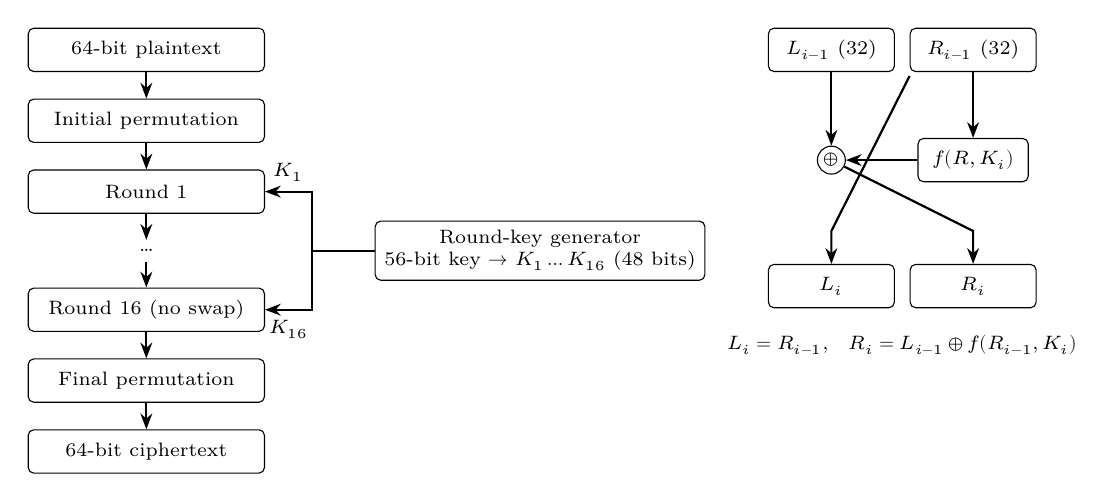
\begin{tikzpicture}[font=\scriptsize,b/.style={draw,rounded corners=2pt,minimum width=3.0cm,minimum height=5.5mm,align=center}]
  \node[b] (p) at (0,0) {64-bit plaintext};
  \node[b] (ip) at (0,-0.9) {Initial permutation};
  \node[b] (r1) at (0,-1.8) {Round 1};
  \node (dots) at (0,-2.55) {\dots};
  \node[b] (r16) at (0,-3.3) {Round 16 (no swap)};
  \node[b] (fp) at (0,-4.2) {Final permutation};
  \node[b] (c) at (0,-5.1) {64-bit ciphertext};
  \foreach \a/\b in {p/ip,ip/r1,r16/fp,fp/c}{\draw[arr] (\a)--(\b);}
  \draw[arr] (r1)--(dots); \draw[arr] (dots)--(r16);
  \node[b,minimum width=3.4cm] (kg) at (5.0,-2.55) {Round-key generator\\56-bit key $\to$ $K_1 \dots K_{16}$ (48 bits)};
  \draw[arr] (kg.west) -- ++(-0.8,0) |- (r1.east) node[pos=0.75,above]{$K_1$};
  \draw[arr] (kg.west) -- ++(-0.8,0) |- (r16.east) node[pos=0.75,below]{$K_{16}$};
  \begin{scope}[xshift=9.6cm]
  \node[b,minimum width=1.6cm] (L) at (-0.9,0) {$L_{i-1}$ (32)};
  \node[b,minimum width=1.6cm] (R) at (0.9,0) {$R_{i-1}$ (32)};
  \node[draw,circle,inner sep=1pt] (x) at (-0.9,-1.4) {$\oplus$};
  \node[b,minimum width=1.4cm] (f) at (0.9,-1.4) {$f(R, K_i)$};
  \draw[arr] (L)--(x); \draw[arr] (R)--(f); \draw[arr] (f)--(x);
  \node[b,minimum width=1.6cm] (L2) at (-0.9,-3.0) {$L_i$};
  \node[b,minimum width=1.6cm] (R2) at (0.9,-3.0) {$R_i$};
  \draw[arr] (x) -- (0.9,-2.3) -- (R2); \draw[arr] (R.south west) ++(0,-0.05) -- (-0.9,-2.3) -- (L2);
  \node[align=center] at (0,-3.75) {$L_i = R_{i-1}$, \; $R_i = L_{i-1} \oplus f(R_{i-1}, K_i)$};
  \end{scope}
\end{tikzpicture}
\end{center}

\subsection{Initial and final permutations}
Keyless straight P-boxes, inverses of each other, with \textbf{no cryptographic significance}. IP table starts \ttx{58 50 42 34 26 18 10 02 | 60 52 44 \dots}: output bit 1 $=$ input bit 58; input bit 1 goes to output 40.\\
\textbf{Example}: input \ttx{0x0002 0000 0000 0001} has only bits 15 and 64 set. In the IP table, 15 is at position 63 and 64 is at position 25 $\Rightarrow$ output \ttx{0x0000 0080 0000 0002} (bits 25 and 63). FP maps it back.

\subsection{The round function $f(R_{i-1}, K_i)$}
\begin{enumerate}[leftmargin=1.5em]
  \item \textbf{Expansion P-box} 32 $\to$ 48: 8 groups of 4 bits become 6 by copying the neighbouring bits (first row \ttx{32 01 02 03 04 05}, last row \ttx{28 29 30 31 32 01}).
  \item \textbf{Whitener}: XOR with the 48-bit round key $K_i$.
  \item \textbf{8 S-boxes}, each \textbf{6 bits $\to$ 4 bits} (the confusion, ``real mixing''). Row $=$ bits 1 and 6 (0--3), column $=$ bits 2--5 (0--15).
  \item \textbf{Straight P-box} 32 $\to$ 32 (\ttx{16 07 20 21 29 12 28 17 \dots}: input bit 16 becomes output bit 1, input bit 7 becomes output bit 2).
\end{enumerate}
\begin{center}\small\setlength{\tabcolsep}{3.5pt}
\begin{tabular}{@{}c|*{16}{c}@{}}
S1 & 0&1&2&3&4&5&6&7&8&9&10&11&12&13&14&15\\ \midrule
0 & 14&4&13&1&2&15&11&8&3&10&6&12&5&9&0&7\\
1 & 0&15&7&4&14&2&13&1&10&6&12&11&9&5&3&8\\
2 & 4&1&14&8&13&6&2&11&15&12&9&7&3&10&5&0\\
3 & 15&12&8&2&4&9&1&7&5&11&3&14&10&0&6&13\\
\end{tabular}
\end{center}
\textbf{Example}: input \ttx{100011} to S1: row $= (1\,1)_2 = 3$, column $= (0001)_2 = 1$ $\Rightarrow$ 12 $=$ \ttx{1100}. (Others: \ttx{000000} $\to$ 14 $=$ \ttx{1110}; \ttx{111111} $\to$ row 3 col 15 $=$ 13 $=$ \ttx{1101}.)

\textbf{Cipher vs.\ reverse cipher}: each round $=$ mixer ($L \oplus f(R, K)$) $+$ swapper; the \textbf{last round has no swapper} so that the reverse cipher is the same algorithm with keys $K_{16} \dots K_1$.

\subsection{Key generation}
64-bit key $\to$ \textbf{parity drop} (removes bits 8, 16, \dots, 64, permutes) $\to$ 56 bits $\to$ split into two 28-bit halves $\to$ each round: \textbf{circular left shift} both halves, combine, \textbf{compression P-box 56 $\to$ 48} $\to$ $K_i$.\\
Shifts: \textbf{1 bit in rounds 1, 2, 9, 16}; 2 bits in the others (total 28, so the halves return to the start).

\subsection{Analysis and weaknesses}
\begin{itemize}
  \item \textbf{Avalanche effect} (small change in plaintext or key $\to$ big change in ciphertext) and \textbf{completeness} (each ciphertext bit depends on many plaintext bits): DES is strong in both.
  \item \textbf{Design weaknesses}: in S-box 4 three output bits can be derived from the first; two chosen inputs to the S-box array can give the same output; the same round output can come from changing only 3 neighbouring S-boxes; IP/FP add nothing; the expansion repeats the 1st and 4th bit of every 4-bit group.
  \item \textbf{Key size}: $2^{56}$ keys. At $10^6$ keys/s on $10^6$ parallel chips: about \textbf{20 hours}. (The slides' 3500 networked computers took 120 days on an RSA challenge.)
  \item \textbf{Weak keys} (4): all round keys identical (e.g.\ \ttx{0101 0101 0101 0101}, \ttx{FEFE FEFE FEFE FEFE}); encrypting twice gives back the plaintext. \textbf{Semi-weak keys} (6 pairs): only 2 distinct round keys, each used 8 times; one key of a pair decrypts what the other encrypted.
\end{itemize}

\subsection{Multiple DES}
\begin{itemize}
  \item \textbf{Double DES}: $C = E_{K_2}(E_{K_1}(P))$, 112-bit key, but the \textbf{meet-in-the-middle} attack (known plaintext) cuts it to about $2^{57}$ tests: encrypt $P$ under all $2^{56}$ $K_1$ and store the middle values $M$; decrypt $C$ under all $2^{56}$ $K_2$ and look for a match ($M = E_{K_1}(P) = D_{K_2}(C)$).
  \item \textbf{Triple DES, two keys} (EDE): $C = E_{K_1}(D_{K_2}(E_{K_1}(P)))$. With $K_1 = K_2$ it reduces to single DES (backward compatible). \textbf{Three keys}: $E_{K_3}(D_{K_2}(E_{K_1}(P)))$.
\end{itemize}

\begin{examtip}
``Explain DES'' (5--10 marks): block/key/round sizes; the structure diagram; the round (expansion, XOR, S-boxes with the row/column rule, straight P); key generation (parity drop, shifts 1/2, compression); one weakness (key size) and the 3DES fix. A numerical: an S-box lookup or an IP mapping.
\end{examtip}

% College Lecture 9: AES. S-box values, MixColumns and key expansion computed by script (checked against FIPS-197).
\section{Advanced Encryption Standard (AES)}\label{sec:aes}

NIST, December 2001 (Rijndael). \textbf{Non-Feistel}, 128-bit block, round keys always 128 bits.
\begin{center}\small
\begin{tabular}{@{}cccc@{}}
\toprule
Version & Key & Rounds $N_r$ & Round keys / words\\
\midrule
AES-128 & 128 & 10 & 11 / 44\\
AES-192 & 192 & 12 & 13 / 52\\
AES-256 & 256 & 14 & 15 / 60\\
\bottomrule
\end{tabular}
\end{center}
Number of round keys $= N_r + 1$ (one extra AddRoundKey before round 1). Data units: bit, byte, word (4 bytes), block (16 bytes), \textbf{state} ($4 \times 4$ bytes).

\textbf{Block $\to$ state}: filled \textbf{column by column}: $s_{r,c} = b_{r + 4c}$.
\textbf{Example}: \ttx{AES USES A MATRIX} $\to$ \ttx{AESUSESAMATRIXZZ} (two fillers), letters as 0--25:
\[
\text{State} = \begin{pmatrix}00&12&0C&08\\04&04&00&17\\12&12&13&19\\14&00&11&19\end{pmatrix}_{16}
\quad\xrightarrow{\text{SubBytes}}\quad
\begin{pmatrix}63&C9&FE&30\\F2&F2&63&F0\\C9&C9&7D&D4\\FA&63&82&D4\end{pmatrix}
\quad\xrightarrow{\text{ShiftRows}}\quad
\begin{pmatrix}63&C9&FE&30\\F2&63&F0&F2\\7D&D4&C9&C9\\D4&FA&63&82\end{pmatrix}
\]

\subsection{Structure}
Encryption: AddRoundKey($w_0..w_3$); rounds 1 to $N_r - 1$: \textbf{SubBytes, ShiftRows, MixColumns, AddRoundKey}; last round: SubBytes, ShiftRows, AddRoundKey (\textbf{no MixColumns}). Decryption uses the inverse transformations (InvSubBytes, InvShiftRows, InvMixColumns, AddRoundKey) with round keys in reverse order.

\subsection{The four transformations}
\begin{itemize}
  \item \textbf{SubBytes} (substitution, \textbf{intrabyte}): each byte through the same S-box: first row hex digit selects the row, second the column. Same byte in $\to$ same byte out (two \ttx{04}s both become \ttx{F2}). Mathematically: multiplicative inverse in GF$(2^8)$ ($00 \mapsto 00$), then an affine transform with constant \ttx{63}. \ttx{5A} $\to$ \ttx{BE} and \ttx{5B} $\to$ \ttx{39}: inputs differing in 1 bit give outputs differing in 4. InvSubBytes is the inverse table.
  \item \textbf{ShiftRows} (permutation, \textbf{byte exchange}): row $r$ rotates left by $r$ bytes (row 0 unchanged). Byte-level, unlike DES's bit-level permutations. InvShiftRows rotates right.
  \item \textbf{MixColumns} (\textbf{interbyte} mixing): each column is multiplied in GF$(2^8)$ by a constant matrix; inverse uses the inverse matrix.
  \[
  \begin{pmatrix}02&03&01&01\\01&02&03&01\\01&01&02&03\\03&01&01&02\end{pmatrix}
  \qquad\text{inverse:}\qquad
  \begin{pmatrix}0E&0B&0D&09\\09&0E&0B&0D\\0D&09&0E&0B\\0B&0D&09&0E\end{pmatrix}
  \]
  $02 \cdot b$ $=$ left shift, XOR \ttx{1B} if the top bit was 1; \;$03 \cdot b = (02 \cdot b) \oplus b$. FIPS test column \ttx{db 13 53 45} $\to$ \ttx{8e 4d a1 bc}: first byte $= 02{\cdot}db \oplus 03{\cdot}13 \oplus 53 \oplus 45$ $= \ttx{ad} \oplus \ttx{35} \oplus \ttx{53} \oplus \ttx{45} = \ttx{8e}$. (Column 0 of the example state above $\to$ \ttx{62 cf 0c 99}.)
  \item \textbf{AddRoundKey}: XOR each column with a round-key word, $s_c \leftarrow s_c \oplus w_{4\cdot\text{round} + c}$. Self-inverse.
\end{itemize}

\subsection{Key expansion (AES-128)}
\[
w_0..w_3 = \text{cipher key};\qquad
w_i = \begin{cases} w_{i-4} \oplus w_{i-1} & i \bmod 4 \ne 0\\ w_{i-4} \oplus t,\ \ t = \text{SubWord}(\text{RotWord}(w_{i-1})) \oplus \text{RCon}[i/4] & i \bmod 4 = 0\end{cases}
\]
\textbf{RotWord}: rotate the 4 bytes left by one. \textbf{SubWord}: S-box on each byte. \textbf{RCon}: $(x^{j-1} \bmod m(x), 00, 00, 00)$: \ttx{01 02 04 08 10 20 40 80 1B 36} for rounds 1--10.\\
FIPS-197 key \ttx{2b7e1516 28aed2a6 abf71588 09cf4f3c} $\to$ $w_4..w_7 =$ \ttx{a0fafe17 88542cb1 23a33939 2a6c7605} (verified; $w_{43} =$ \ttx{b6630ca6}).

\subsection{Analysis}
Brute force: $2^{128}$ vs.\ DES's $2^{56}$ ($2^{72}$ times harder); no weak keys; strong diffusion and confusion defeat statistical attacks; designed with differential/linear cryptanalysis in mind; simple and cheap to implement.

\begin{center}\small
\begin{tabularx}{\textwidth}{@{}l X X@{}}
\toprule
 & DES & AES\\
\midrule
Structure & Feistel & non-Feistel (all invertible)\\
Block / key & 64 / 56 & 128 / 128, 192, 256\\
Rounds & 16 & 10, 12, 14\\
Works on & bits & bytes (GF$(2^8)$)\\
Permutation & bit-level P-boxes & byte-level ShiftRows\\
\bottomrule
\end{tabularx}
\end{center}

\begin{fixbox}
\begin{itemize}
  \item Example \#1 on the slide writes X as \ttx{23}. X is letter 23 in \emph{decimal}, which is \ttx{17} in hex (the slide correctly converts M $= 12 \to$ \ttx{0C} and R $= 17 \to$ \ttx{11}). With \ttx{17}, SubBytes gives \ttx{F0}; the slide's \ttx{26} is the S-box of \ttx{23}. If the exam reuses the slide's state, say which value you used.
\end{itemize}
\end{fixbox}

% College Lecture 12: asymmetric-key cryptography and RSA. All numbers verified by script.
\section{Asymmetric-Key Cryptography and RSA}

\textbf{Idea}: the \textbf{public key locks, the private key unlocks}. $C = f(K_{\text{public}}, P)$, $P = g(K_{\text{private}}, C)$. Much slower than symmetric ciphers, so it's used for key exchange, authentication and digital signatures rather than bulk data.

\begin{keybox}[title=Trapdoor one-way function]
\textbf{One-way}: $y = f(x)$ easy, $x = f^{-1}(y)$ infeasible. \textbf{Trapdoor}: $f^{-1}$ becomes easy with a secret.\\
$n = pq$ is one-way (factoring). $y = x^k \bmod n$ is a trapdoor one-way function: with the trapdoor $k'$, $kk' \equiv 1 \pmod{\phi(n)}$, recover $x = y^{k'} \bmod n$.
\end{keybox}

\subsection{RSA (Rivest, Shamir, Adleman)}
\begin{keybox}[title={Key generation, encryption, decryption}]
1.\ Choose large primes $p \ne q$; \;$n = pq$; \;$\phi(n) = (p - 1)(q - 1)$.\\
2.\ Choose $e$ with $1 < e < \phi(n)$, $\gcd(e, \phi(n)) = 1$. \;3.\ $d = e^{-1} \bmod \phi(n)$ (extended Euclid).\\
Public key $(e, n)$; private key $d$.
\qquad Encrypt: $C = P^e \bmod n$ \;($P < n$). \qquad Decrypt: $P = C^d \bmod n$.
\end{keybox}
\textbf{Why it works}: $ed = k\phi(n) + 1$, so $C^d = P^{ed} = P^{k\phi(n)+1} \equiv P \pmod n$ (Euler, second version). RSA uses a public ring $\langle \mathbb{Z}_n, +, \times\rangle$ for encryption/decryption and a private group $\langle \mathbb{Z}_{\phi(n)}^*, \times\rangle$ for key generation.

\begin{center}\small
\begin{tabular}{@{}lllllll@{}}
\toprule
$p, q$ & $n$ & $\phi(n)$ & $e$ & $d$ & $P \to C$ & $C \to P$\\
\midrule
7, 11 & 77 & 60 & 13 & 37 & $5^{13} \bmod 77 = 26$ & $26^{37} \bmod 77 = 5$\\
7, 11 & 77 & 60 & 13 & 37 & $63^{13} \bmod 77 = 28$ & $28^{37} \bmod 77 = 63$\\
17, 11 & 187 & 160 & 7 & 23 & $88^{7} \bmod 187 = 11$ & $11^{23} \bmod 187 = 88$\\
3, 11 & 33 & 20 & 7 & 3 & $5^7 \bmod 33 = 14$ & $14^3 \bmod 33 = 5$\\
\bottomrule
\end{tabular}
\end{center}
Finding $d$ for $(e, \phi) = (7, 160)$: extended Euclid gives $160 = 22\cdot7 + 6$, $7 = 1\cdot6 + 1$, back-substitute: $1 = 7 - 6 = 7 - (160 - 22\cdot7) = 23\cdot7 - 160$ $\Rightarrow d = 23$.

\subsection{Attacks and recommendations}
Potential attacks (none devastating so far): \textbf{factorization} of $n$; \textbf{chosen-ciphertext}; on the \textbf{encryption exponent} (low $e$: Coppersmith, broadcast, related messages, short pad); on the \textbf{decryption exponent} (revealed or low $d$); \textbf{plaintext} (short message, cyclic, unconcealed); \textbf{common modulus}; \textbf{implementation} (timing, power).
\begin{itemize}
  \item $n$ at least \textbf{1024 bits} (309 digits); $p$, $q$ at least \textbf{512 bits} each, \textbf{not close} to each other (Fermat factoring), $p - 1$ and $q - 1$ with at least one large prime factor (Pollard $p - 1$), $p/q$ not close to a simple fraction.
  \item Never share $n$ between users. $e = 2^{16} + 1 = 65537$ or close to it.
  \item If $d$ leaks, change $n$, $e$ and $d$ (knowing $n$ and one $(e, d)$ pair lets you factor $n$).
  \item Pad messages with \textbf{OAEP}.
\end{itemize}

\begin{trap}[: the usual slips]
$d$ is the inverse of $e$ mod $\boldsymbol{\phi(n)}$, not mod $n$. The plaintext must be $< n$. $e$ must be coprime to $\phi(n)$, so $e = 2$ never works ($\phi(n)$ is even).
\end{trap}

% College Lecture 13: ElGamal and ECC. All points and values verified by script.
\section{ElGamal and Elliptic Curve Cryptosystems}

\subsection{ElGamal}
Security rests on the \textbf{discrete logarithm problem}: $e_2 = e_1^d \bmod p$ is easy; finding $d = \log_{e_1} e_2 \bmod p$ is infeasible for large $p$.
\begin{keybox}[title=ElGamal]
\textbf{Keys}: large prime $p$; $e_1$ a primitive root mod $p$; private $d$ with $1 \le d \le p - 2$; \;$e_2 = e_1^d \bmod p$. Public $(e_1, e_2, p)$, private $d$.\\
\textbf{Encrypt} (fresh random $r$): $C_1 = e_1^r \bmod p$, \;$C_2 = P \cdot e_2^r \bmod p$.\\
\textbf{Decrypt}: $P = C_2 \cdot (C_1^d)^{-1} \bmod p$. \;Proof: $C_1^d = e_1^{rd} = e_2^r$, so $C_2 (C_1^d)^{-1} = P e_2^r (e_2^r)^{-1} = P$.
\end{keybox}
\textbf{Example}: $p = 11$, $e_1 = 2$, $d = 3$ $\Rightarrow e_2 = 8$. Alice sends $P = 7$ with $r = 4$: $C_1 = 2^4 \bmod 11 = 5$, \;$C_2 = 7 \cdot 8^4 \bmod 11 = 7 \cdot 4096 \bmod 11 = 6$. Bob: $C_1^d = 5^3 \bmod 11 = 4$, $4^{-1} = 3$, $P = 6 \cdot 3 \bmod 11 = \mathbf{7}$.\\
\textbf{Shortcut}: $(C_1^d)^{-1} = C_1^{p-1-d}$ (Fermat): $5^{7} \bmod 11 = 3$ \checkmark.

\textbf{Security}: \textbf{low-modulus attack} (small $p$ lets Eve solve the discrete log once and decrypt everything; use $p \ge 1024$ bits); \textbf{known-plaintext attack} if $r$ is reused: from $C_2 = P e_2^r$ she gets $e_2^r = C_2 P^{-1}$, then $P' = C_2' (e_2^r)^{-1}$. Use a fresh $r$ every time. Note the ciphertext is twice the size of the plaintext.

\subsection{Elliptic curves over $\mathbb{Z}_p$}
RSA and ElGamal need big keys; ECC gives the same security with much smaller keys (160-bit ECC $\approx$ 1024-bit RSA).
\[
E_p(a, b):\ y^2 \equiv x^3 + ax + b \pmod p,\quad p > 3,\quad 4a^3 + 27b^2 \not\equiv 0 \pmod p,\ \text{ plus the point at infinity } O.
\]
\textbf{Finding points}: for each $x$, compute $w = x^3 + ax + b \bmod p$; if $w$ is a square mod $p$, the points are $(x, \pm\sqrt w)$. $E_{13}(1,1)$:
\begin{center}\small
\ttx{(0,1) (0,12) (1,4) (1,9) (4,2) (4,11) (5,1) (5,12) (7,0) (8,1) (8,12) (10,6) (10,7) (11,2) (11,11) (12,5) (12,8)}
\end{center}
17 points $+ O = 18$. $x = 2, 3, 6, 9$ give non-squares. Inverse of $(x, y)$ is $(x, -y) = (x, p - y)$; $(7, 0)$ is its own inverse.

\begin{keybox}[title=Point addition and doubling]
$R = P + Q$: \quad $x_3 = s^2 - x_1 - x_2$, \quad $y_3 = s(x_1 - x_3) - y_1 \pmod p$, where
\[
s = \frac{y_2 - y_1}{x_2 - x_1}\ (P \ne Q,\ \text{addition}),\qquad s = \frac{3x_1^2 + a}{2y_1}\ (P = Q,\ \text{doubling}).
\]
Division means multiplying by the inverse mod $p$. $P + (-P) = O$; $P + O = P$.
\end{keybox}
\textbf{Doubling on $E_{17}(2, 2)$}, $P = (5, 1)$: $s = (3 \cdot 25 + 2) \cdot (2)^{-1} = 77 \cdot 9 \equiv 9 \cdot 9 = 81 \equiv 13$; \;$x_3 = 169 - 10 = 159 \equiv 6$; \;$y_3 = 13(5 - 6) - 1 = -14 \equiv 3$ $\Rightarrow 2P = (6, 3)$. (This $P$ generates all 19 points of the curve.)

\textbf{Scalar multiplication} $kP = P + \dots + P$: in $E_{13}(1,1)$, $4 \cdot (1, 4) = (11, 11)$ and $3 \cdot (8, 1) = (10, 7)$.

\textbf{Hasse}: $p + 1 - 2\sqrt p \le \#E \le p + 1 + 2\sqrt p$. \textbf{ECDLP}: given $P$ and $T = dP$, find $d$; best known method is Pollard rho, infeasible for large curves.

\subsection{ECC simulating ElGamal}
\begin{keybox}
\textbf{Keys}: curve $E$, point $e_1$, private $d$, \;$e_2 = d \times e_1$. Public $(E, e_1, e_2)$.\\
\textbf{Encrypt} (plaintext is a point $P$, random $r$): $C_1 = r \times e_1$, \;$C_2 = P + r \times e_2$.\\
\textbf{Decrypt}: $P = C_2 - d \times C_1$ \;(subtract $=$ add the inverse point), since $d \times r \times e_1 = r \times e_2$.
\end{keybox}
\textbf{Example} $E_{67}(2, 3)$: $e_1 = (2, 22)$, $d = 4$ $\Rightarrow e_2 = (13, 45)$. Alice: $P = (24, 26)$, $r = 2$: $C_1 = (35, 1)$, $C_2 = (21, 44)$. Bob: $4 \times C_1 = (23, 25)$, inverse $(23, 42)$, $(21, 44) + (23, 42) = \mathbf{(24, 26)}$ \checkmark.

\begin{trap}[: point arithmetic slips]
The doubling slope has $3x_1^2 + a$ (uses $a$, never $b$). Compute $s$ mod $p$ with a modular inverse, never a fraction. $-P$ flips only $y$.
\end{trap}

% College Lecture 14: message integrity, birthday problems, hash attacks, iterated hashes, SHA-512, Whirlpool. Numbers verified by script.
\section{Message Integrity and Hash Functions}

Integrity without secrecy (a published will must not be altered). Electronic equivalent of document $+$ fingerprint: \textbf{message $+$ message digest}, the digest made by a \textbf{cryptographic hash function}. To check: recompute the digest and compare with the stored one.

\subsection{Three criteria}
\begin{center}\small
\begin{tabularx}{\textwidth}{@{}l X X@{}}
\toprule
Criterion & Eve is given\dots & \dots and must not be able to find\\
\midrule
\textbf{Preimage resistance} & a digest $y = h(M)$ & any $M'$ with $h(M') = y$\\
\textbf{Second preimage resistance} & $M$ and $h(M)$ & $M' \ne M$ with $h(M') = h(M)$ (forging a specific message)\\
\textbf{Collision resistance} & nothing & any pair $M \ne M'$ with $h(M) = h(M')$\\
\bottomrule
\end{tabularx}
\end{center}
A lossless compressor isn't a hash (it's reversible); a checksum isn't (not preimage resistant).

\subsection{The four birthday problems}
$N$ equally likely values, $k$ samples; ``likely'' means $P \ge 1/2$.
\begin{center}\small
\begin{tabular}{@{}lllll@{}}
\toprule
Problem (find $k$ so it's likely that\dots) & $P$ & $k$ at $P = 1/2$ & $N = 365$ & Attack\\
\midrule
1. one sample equals a \emph{predefined} value & $1 - e^{-k/N}$ & $0.69N$ & 253 & preimage\\
2. one equals a sample \emph{chosen from the set} & $1 - e^{-(k-1)/N}$ & $0.69N + 1$ & 254 & second preimage\\
3. \textbf{any two} samples are equal (birthday paradox) & $1 - e^{-k(k-1)/2N}$ & $1.18\sqrt N$ & 23 & collision\\
4. a sample of set 1 equals one of set 2 & $1 - e^{-k^2/N}$ & $0.83\sqrt N$ & 16 & alternate collision\\
\bottomrule
\end{tabular}
\end{center}
Constants: $0.69 = \ln 2$, $1.18 = \sqrt{2\ln 2}$, $0.83 = \sqrt{\ln 2}$. Problems 1, 2 grow like $N$; 3, 4 like $\sqrt N$, so \textbf{collisions are far easier to find than preimages}. (Exact: 23 people give $P = 0.507$.)

\subsection{Random oracle model}
An ideal hash: (1) a new message gets a fixed-length digest chosen \textbf{truly at random} (e.g.\ by coin flips), recorded in a table; (2) a repeated message gets its recorded digest; (3) each new digest is independent of all previous ones, so \textbf{no formula} may be used. Slide example: 16 flips \ttx{HHTHHHTTHTHHTTTH} (H $= 1$) $\to$ \ttx{1101110010110001} $=$ \ttx{DCB1}. A formula like $h(M) = M \bmod n$ fails rule 3: $h(M_1 + M_2) = [h(M_1) + h(M_2)] \bmod n$ is predictable.

\subsection{Attacks on an $n$-bit digest ($N = 2^n$)}
\begin{center}\small
\begin{tabular}{@{}llll@{}}
\toprule
Attack & Eve's algorithm & $k$ for $P = 1/2$ & Order\\
\midrule
Preimage & hash $k$ random messages, compare with $D$ & $0.69 \times 2^n$ & $2^n$\\
Second preimage & hash $k - 1$ messages, compare with $D = h(M)$ & $0.69 \times 2^n + 1$ & $2^n$\\
Collision & hash $k$ messages, compare all pairs & $1.18 \times 2^{n/2}$ & $2^{n/2}$\\
Alternate collision & $k$ meaningful variants of $M$ and of bogus $M'$, compare across & $0.83 \times 2^{n/2}$ & $2^{n/2}$\\
\bottomrule
\end{tabular}
\end{center}
\textbf{64-bit digest}: preimage needs $0.69 \times 2^{64}$ digests; at $2^{30}$/s that is $0.69 \times 2^{34}$ s $\approx$ \textbf{376 years} (secure). Collision needs $1.18 \times 2^{32}$; at $2^{20}$/s, $1.18 \times 2^{12}$ s $\approx$ \textbf{1.3 hours} (\textbf{not} secure). Hence digests $\ge 160$ bits; MD5's 128 bits gives only $2^{64}$ collision security.
\textbf{Alternate collision}: real attacks need \emph{meaningful} pairs, so Eve makes variants (extra spaces, synonyms) of both the genuine and the fake message.

\subsection{Iterated hash functions}
A fixed-size \textbf{compression function} $f$ applied repeatedly. \textbf{Merkle--Damg\aa rd}: append padding and the length; split into $t$ blocks of $n$ bits; $H_0 = $ IV; $H_i = f(H_{i-1}, M_i)$; digest $= H_t$. Collision resistant if $f$ is.
\begin{itemize}
  \item \textbf{From scratch}: MD family (MD2, MD4, \textbf{MD5}: 512-bit blocks, 128-bit digest, too short against collisions); SHA family.
  \item \textbf{From a block cipher}: \textbf{Rabin} ($H_i = E_{M_i}(H_{i-1})$: block as key, previous digest as plaintext; digest size $=$ cipher block, only 64 bits with DES; vulnerable to meet-in-the-middle); \textbf{Davies--Meyer} (Rabin $+$ feed-forward: $H_i = E_{M_i}(H_{i-1}) \oplus H_{i-1}$); \textbf{Miyaguchi--Preneel} (plaintext, key and ciphertext all XORed together; used by Whirlpool).
\end{itemize}
\begin{center}\small
\begin{tabular}{@{}lccccc@{}}
\toprule
 & SHA-1 & SHA-224 & SHA-256 & SHA-384 & SHA-512\\
\midrule
Max message & $2^{64} - 1$ & $2^{64} - 1$ & $2^{64} - 1$ & $2^{128} - 1$ & $2^{128} - 1$\\
Block & 512 & 512 & 512 & 1024 & 1024\\
Digest & 160 & 224 & 256 & 384 & 512\\
Rounds & 80 & 64 & 64 & 80 & 80\\
Word & 32 & 32 & 32 & 64 & 64\\
\bottomrule
\end{tabular}
\end{center}

\subsection{SHA-512}
\begin{itemize}
  \item 1024-bit blocks, 512-bit digest, word $=$ 64 bits; digest $=$ 8 words A--H (initialised from fixed constants).
  \item \textbf{Padding} (Forouzan): padding (a 1 then 0s) plus a \textbf{128-bit length field} make the length a multiple of 1024: $|P| = (-|M| - 128) \bmod 1024$, so $0 \le |P| \le 1023$. $|M| = 2590 \Rightarrow |P| = 354$, total $3 \times 1024$. A message that is already a multiple of 1024 still needs padding (for the length field). (The real standard always adds at least the single 1 bit, so $|M| = 896$ needs a whole extra block.)
  \item \textbf{Word expansion}: 16 words $\to$ 80: $W_i = W_{i-16} \oplus \mathrm{RotShift}_{1\text{-}8\text{-}7}(W_{i-15}) \oplus W_{i-7} \oplus \mathrm{RotShift}_{19\text{-}61\text{-}6}(W_{i-2})$, where $\mathrm{RotShift}_{l\text{-}m\text{-}n}(x) = \mathrm{RotR}_l(x) \oplus \mathrm{RotR}_m(x) \oplus \mathrm{ShL}_n(x)$.
  \item \textbf{Compression}: 80 rounds, each mixing A--H with $W_i$ and a constant $K_i$ using \textbf{Majority}$(x,y,z) = (x \wedge y) \oplus (y \wedge z) \oplus (z \wedge x)$, \textbf{Conditional}$(x,y,z) = (x \wedge y) \oplus (\bar x \wedge z)$, \textbf{Rotate}$(x) = \mathrm{RotR}_{28}(x) \oplus \mathrm{RotR}_{34}(x) \oplus \mathrm{RotR}_{39}(x)$; then \textbf{final adding} of the saved A--H (mod $2^{64}$).
\end{itemize}
\textbf{Class exercises} (slides use a 128-bit $x$ = \ttx{1234 5678 ABCD 2345 3456 5678 ABCD 2468}; verified):
\begin{center}\small
\begin{tabular}{@{}ll@{}}
$\mathrm{RotR}_{12}(x)$ & \ttx{4681 2345 678A BCD2 3453 4565 678A BCD2}\\
$\mathrm{ShL}_{12}(x)$ & \ttx{4567 8ABC D234 5345 6567 8ABC D246 8000}\\
Conditional$(x, y, z)$, $y$, $z$ start with 2, 3 & \ttx{2234 5678 \dots} (first digit: Cond$(1,2,3) = 0010 = 2$)\\
Majority$(x, y, z)$ & \ttx{3234 5678 \dots} (first digit: Maj$(1,2,3) = 0011 = 3$)\\
Rotate$(x)$ & \ttx{6776 95D3 F7EC 1AB8 6776 E6C4 8218 5EB8}\\
\end{tabular}
\end{center}

\textbf{Whirlpool} (NESSIE): iterated hash based on \textbf{Miyaguchi--Preneel}, using a \textbf{modified AES} block cipher as the compression function; 512-bit blocks and digest; the message is padded to an odd multiple of 256 bits plus a 256-bit length field.

\begin{fixbox}
\begin{itemize}
  \item Slide 27: ``0.69 $\times 2^{34}$ seconds or more than 500 years'': $0.69 \times 2^{34}$ s $\approx 376$ years ($2^{34}$ s alone is $\approx 544$). The conclusion (secure) stands.
  \item Slides 54--55 swap the binary for the first digit: Conditional$(0001, 0010, 0011) = 0010 = 2$ and Majority $= 0011 = 3$ (the slide prints them the other way round, though the hex results 2 and 3 are right).
  \item The exercise $x$ is 128 bits, though real SHA-512 words are 64 bits; the rotations on the slide are done on 128 bits.
\end{itemize}
\end{fixbox}

% MNNIT CSN15403 mid-semester papers 2024-25 and 2025-26, fully solved, plus a mock paper in the same style
\clearpage
\section{Previous Year Papers (MNNIT, CSN15403), Fully Solved}\label{sec:pastpapers}

\begin{keybox}[title=What these papers tell you]
\begin{itemize}
  \item \textbf{Format:} 90 minutes, 25 marks, 5--7 questions, ``precise answer with proper justification''. Show every step: tables, matrices, divisions.
  \item \textbf{Sources:} questions come almost word for word from the two standard textbooks: \textbf{Forouzan} (Eve/Alice, $\mathbb{Z}_{100}$, keyed transposition, multiplicative/affine/auto-key, GF$(2^8)$ inverse) and \textbf{Stallings} (``sendmoremoney'' one-time pad, the AES state values).
  \item \textbf{Repeat topics:} Playfair (both years), GF$(2^8)$ inverse (both years), extended Euclid (inverse / Diophantine, both years), DES/AES (both years).
\end{itemize}
\end{keybox}
\begin{center}\small
\begin{tabularx}{\textwidth}{@{}l c c X@{}}
\toprule
Topic & 2024--25 & 2025--26 & In these notes?\\
\midrule
Playfair encryption & 3 & 4 & Section~\ref{sec:playfair}\\
One-time pad / Vigen\`ere & -- & 8 & Sections~\ref{sec:poly}, \ref{sec:otp}\\
Cipher properties, attack types, keyed transposition & 2 + 3 & -- & Sections~\ref{sec:attacks}, \ref{sec:classextra}\\
Modular arithmetic, exponentiation, inverses & 3 & -- & Sections~\ref{sec:modular}--\ref{sec:fermat}\\
Extended Euclid / Diophantine & 5 & 3 & Section~\ref{sec:exteuclid}\\
GF$(2^8)$ polynomial inverse & 4 & 4 & Section~\ref{sec:algebra}\\
DES (Feistel, round function, key schedule) & 5 & -- & Section~\ref{sec:des}\\
AES (ShiftRows, AddRoundKey) & -- & 6 & Section~\ref{sec:aes}\\
\bottomrule
\end{tabularx}
\end{center}
Every topic in these papers is now covered in its own section; the boxes below are one-page summaries for quick revision.

\subsection{Quick-revision method boxes}

\begin{keybox}[title={Extended Euclidean algorithm (Forouzan table): inverse of $b$ mod $n$}]
Columns $q, r_1, r_2, r, t_1, t_2, t$. Start with $r_1 = n$, $r_2 = b$, $t_1 = 0$, $t_2 = 1$. Each row:
\[
q = \lfloor r_1 / r_2 \rfloor,\quad r = r_1 - q\,r_2,\quad t = t_1 - q\,t_2;\qquad\text{then shift: } r_1 \leftarrow r_2,\; r_2 \leftarrow r,\; t_1 \leftarrow t_2,\; t_2 \leftarrow t.
\]
Stop when $r_2 = 0$. If $r_1 = 1$, then $b^{-1} = t_1 \bmod n$. If $r_1 \ne 1$, there is \textbf{no inverse} ($\gcd \ne 1$).
\textbf{Pseudocode:}
\texttt{r1=n; r2=b; t1=0; t2=1; while r2>0 \{ q=r1/r2; r=r1-q*r2; r1=r2; r2=r; t=t1-q*t2; t1=t2; t2=t \}; if r1==1 return t1 mod n}
\end{keybox}

\begin{keybox}[title={Linear Diophantine equation $ax + by = c$}]
Let $d = \gcd(a, b)$. If $d \nmid c$: \textbf{no solution}. Otherwise divide by $d$, find $s, t$ with $as + bt = d$ (extended Euclid), and multiply by $c/d$ to get a particular solution $(x_0, y_0)$.
\textbf{General solution:} $x = x_0 + \frac{b}{d}k$, \; $y = y_0 - \frac{a}{d}k$ \; ($k \in \mathbb{Z}$).
\end{keybox}

\begin{keybox}[title={GF$(p)$ and GF$(2^8)$}]
\textbf{GF$(p)$} = $\{0, \dots, p-1\}$ with $+$ and $\times$ mod a prime $p$. Every non-zero element has an inverse, and ``$a \div b$'' means $a \times b^{-1}$.
\textbf{GF$(2^8)$} elements are polynomials of degree $<8$ with coefficients 0/1 (one byte). \textbf{Add = XOR} (so $+$ and $-$ are the same). Multiply polynomials, then reduce mod $m(x) = x^8 + x^4 + x^3 + x + 1$.
\textbf{Inverse:} the same extended-Euclid table with polynomial division, where every subtraction is an XOR.
\end{keybox}

\begin{keybox}[title=Two classical ciphers and the attack types]
\textbf{Multiplicative:} $C = k_1 P \bmod 26$, with $\gcd(k_1, 26) = 1$. \textbf{Affine:} $C = (k_1 P + k_2) \bmod 26$, decrypted by $P = k_1^{-1}(C - k_2)$.
\textbf{Attacks:} \emph{ciphertext-only} (Eve has only ciphertext), \emph{known-plaintext} (has some plaintext--ciphertext pairs), \emph{chosen-plaintext} (can encrypt plaintext of her choice), \emph{chosen-ciphertext} (can decrypt ciphertext of her choice).
\end{keybox}

% ================================================================
\subsection{Mid-Sem 2024--25, solved}

\textbf{Q1 (2).} \emph{Max characters changed in the ciphertext if one plaintext character changes: (a) multiplicative (b) affine (c) Vigen\`ere (d) auto-key.}\\
(a) \textbf{1}, (b) \textbf{1}, (c) \textbf{1}: each encrypts one character on its own (Vigen\`ere uses a different shift per position, but still one character in, one out).
(d) \textbf{2}. In auto-key the plaintext is also the key: $k_{i+1} = P_i$ (Forouzan; or $k_{i+m} = P_i$ with an $m$-letter keyword, as in our lecture). So changing $P_i$ changes $C_i$ and the one later character it acts as key for.

\textbf{Q2 (3).} \emph{Playfair, key ``GUIDANCE'': ``The key is hidden under the door pad''.}
\begin{center}\small
\begin{minipage}[c]{0.25\textwidth}\centering
\begin{tabular}{|*{5}{c|}}\hline G&U&I/J&D&A\\\hline N&C&E&B&F\\\hline H&K&L&M&O\\\hline P&Q&R&S&T\\\hline V&W&X&Y&Z\\\hline\end{tabular}
\end{minipage}
\begin{minipage}[c]{0.7\textwidth}
Digrams (\ttx{dd} $\to$ \ttx{dx}; \ttx{oo} $\to$ \ttx{ox}; odd length, so the final \ttx{d} becomes \ttx{dx}):\\
\ttx{th ek ey is hi dx de nu nd er th ed ox or pa dx}\\[2pt]
\ttx{PO CL BX DR LG IY IB CG BG LX PO BI LZ LT TG IY}\\[2pt]
(\ttx{er}$\to$\ttx{LX} is a column case; all the others are rectangles.)
\end{minipage}
\end{center}
Ciphertext: \textbf{\ttx{POCLBXDRLGIYIBCGBGLXPOBILZLTTGIY}}.

\textbf{Q3 (3).} \emph{Eve types ``abcdefghij'' on Alice's machine and sees ``CABDEHFGIJ''. Keyed transposition.}\\
(a) \textbf{Chosen-plaintext attack}: Eve chooses the plaintext and sees its encryption.
(b) The pattern repeats every 5: \ttx{abcde}$\to$\ttx{CABDE} and \ttx{fghij}$\to$\ttx{HFGIJ} (positions 3, 1, 2, 4, 5 both times). So the \textbf{key size is 5}.
Encryption key: output takes input positions \textbf{(3 1 2 4 5)}. Decryption key = inverse permutation \textbf{(2 3 1 4 5)}.

\textbf{Q4 (4).} \emph{Inverse of $x^5$ in GF$(2^8)$ mod $m = x^8 + x^4 + x^3 + x + 1$.}
\begin{center}\small\setlength{\tabcolsep}{3pt}
\begin{tabular}{@{}lllllll@{}}
\toprule
$q$ & $r_1$ & $r_2$ & $r$ & $t_1$ & $t_2$ & $t$\\
\midrule
$x^3$ & $x^8{+}x^4{+}x^3{+}x{+}1$ & $x^5$ & $x^4{+}x^3{+}x{+}1$ & 0 & 1 & $x^3$\\
$x{+}1$ & $x^5$ & $x^4{+}x^3{+}x{+}1$ & $x^3{+}x^2{+}1$ & 1 & $x^3$ & $x^4{+}x^3{+}1$\\
$x$ & $x^4{+}x^3{+}x{+}1$ & $x^3{+}x^2{+}1$ & 1 & $x^3$ & $x^4{+}x^3{+}1$ & $x^5{+}x^4{+}x^3{+}x$\\
$x^3{+}x^2{+}1$ & $x^3{+}x^2{+}1$ & 1 & 0 & $x^4{+}x^3{+}1$ & $x^5{+}x^4{+}x^3{+}x$ & $m$\\
 & \textbf{1} & 0 & & $\mathbf{x^5{+}x^4{+}x^3{+}x}$ & & \\
\bottomrule
\end{tabular}
\end{center}
$(x^5)^{-1} = \mathbf{x^5 + x^4 + x^3 + x}$ (byte \ttx{3A}).
Check: using $x^8 = x^4{+}x^3{+}x{+}1$, $x^9 = x^5{+}x^4{+}x^2{+}x$, $x^{10} = x^6{+}x^5{+}x^3{+}x^2$:
$x^5(x^5{+}x^4{+}x^3{+}x) = x^{10}{+}x^9{+}x^8{+}x^6$, and every term cancels in pairs except 1 \checkmark.

\textbf{Q5 (3).}
(i) GF(7): $5 \div 3 = 5 \times 3^{-1} = 5 \times 5 = 25 \equiv \mathbf{4}$ (since $3 \cdot 5 = 15 \equiv 1$).
(ii) $100^{95} \bmod 9$: $100 \equiv 1$, so the answer is $\mathbf{1}$.
$658^{17} \bmod 17$: $658 = 38\cdot17 + 12$, and by Fermat $a^{17} \equiv a \pmod{17}$, so the answer is $\mathbf{12}$.
$145^{102} \bmod 101$: $145 \equiv 44$; Fermat gives $44^{100} \equiv 1$, so $44^{102} \equiv 44^2 = 1936 = 19\cdot101 + 17$, i.e.\ $\mathbf{17}$.
(iii) $7^{-1} \bmod 17 = \mathbf{5}$ ($35 = 2\cdot17 + 1$). $15^{-1} \bmod 99$: $\gcd(15, 99) = 3 \ne 1$, so it \textbf{does not exist}. (That's the trap.)

\textbf{Q6 (5). DES: Feistel structure, round function, key generation.}
\begin{center}
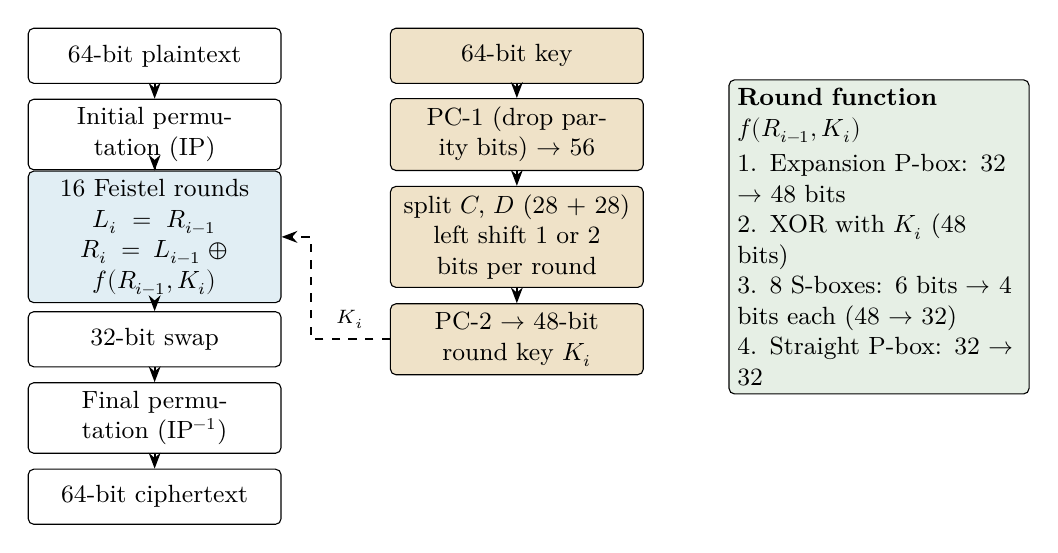
\begin{tikzpicture}[every node/.style={font=\scriptsize}, bx/.style={box,minimum width=30mm,text width=30mm}]
  % data path
  \node[bx] (p) at (0,0) {64-bit plaintext};
  \node[bx] (ip) at (0,-1) {Initial permutation (IP)};
  \node[bx,fill=cyan!10] (r) at (0,-2.3) {16 Feistel rounds\\$L_i = R_{i-1}$\\$R_i = L_{i-1} \oplus f(R_{i-1}, K_i)$};
  \node[bx] (sw) at (0,-3.6) {32-bit swap};
  \node[bx] (fp) at (0,-4.6) {Final permutation (IP$^{-1}$)};
  \node[bx] (c) at (0,-5.6) {64-bit ciphertext};
  \foreach \u/\v in {p/ip,ip/r,r/sw,sw/fp,fp/c} \draw[arr] (\u)--(\v);
  % key schedule
  \node[bx,fill=yellow!20] (k) at (4.6,0) {64-bit key};
  \node[bx,fill=yellow!20] (pc1) at (4.6,-1) {PC-1 (drop parity bits) $\to$ 56};
  \node[bx,fill=yellow!20] (sh) at (4.6,-2.3) {split $C$, $D$ (28 + 28)\\left shift 1 or 2 bits per round};
  \node[bx,fill=yellow!20] (pc2) at (4.6,-3.6) {PC-2 $\to$ 48-bit round key $K_i$};
  \foreach \u/\v in {k/pc1,pc1/sh,sh/pc2} \draw[arr] (\u)--(\v);
  \draw[arr,dashed] (pc2.west) -- node[above]{$K_i$} ++(-1.0,0) |- (r.east);
  % round function
  \node[box,fill=green!12,text width=36mm,align=left] (f) at (9.2,-2.3) {\textbf{Round function} $f(R_{i-1}, K_i)$\\[2pt]
    1. Expansion P-box: 32 $\to$ 48 bits\\2. XOR with $K_i$ (48 bits)\\3. 8 S-boxes: 6 bits $\to$ 4 bits each (48 $\to$ 32)\\4. Straight P-box: 32 $\to$ 32};
\end{tikzpicture}
\end{center}
\begin{itemize}
  \item \textbf{Feistel structure:} each round changes only one half and then swaps the halves. Decryption is the \emph{same} algorithm with the round keys used in reverse ($K_{16}, \dots, K_1$). $f$ need not be invertible.
  \item \textbf{Shifts:} 1 bit in rounds 1, 2, 9, 16; 2 bits in all the others (28 bits in total).
\end{itemize}
\begin{minipage}[t]{0.48\textwidth}\small
\textbf{S-box substitution (pseudocode)}\\
\ttfamily for i = 1 to 8:\\
\hspace*{1em}b = in[6i-5 .. 6i]\quad // 6 bits\\
\hspace*{1em}row = 2*b1 + b6\quad // outer bits\\
\hspace*{1em}col = b2b3b4b5\quad // inner 4 bits\\
\hspace*{1em}out[4i-3 .. 4i] = S[i][row][col]\\
return out\quad // 32 bits
\end{minipage}\hfill
\begin{minipage}[t]{0.48\textwidth}\small
\textbf{Key generation (pseudocode)}\\
\ttfamily K56 = PC1(K64)\\
C = K56[1..28]; D = K56[29..56]\\
for i = 1 to 16:\\
\hspace*{1em}s = (i in \{1,2,9,16\}) ? 1 : 2\\
\hspace*{1em}C = rotl(C, s); D = rotl(D, s)\\
\hspace*{1em}K[i] = PC2(C || D)\quad // 48 bits\\
return K[1..16]
\end{minipage}

\medskip
\textbf{Q7 (5).} \emph{Pseudocode for finding an inverse, and finding $23^{-1}$ in $\mathbb{Z}_{100}$.}
This is the \textbf{extended Euclidean algorithm} (pseudocode in the method box). Mr X's worry is real: an inverse exists only when $\gcd = 1$, and the same algorithm tells him so when it doesn't. Here $\gcd(100, 23) = 1$:
\begin{center}\small
\begin{tabular}{@{}cccccccc@{}}
\toprule
Iter. & $q$ & $r_1$ & $r_2$ & $r$ & $t_1$ & $t_2$ & $t$\\
\midrule
1 & 4 & 100 & 23 & 8 & 0 & 1 & $-4$\\
2 & 2 & 23 & 8 & \textbf{7} & 1 & $-4$ & 9\\
3 & 1 & 8 & 7 & 1 & $-4$ & 9 & $\mathbf{-13}$\\
4 & 7 & 7 & 1 & 0 & 9 & $-13$ & \textbf{100}\\
 & & \textbf{1} & 0 & & $\mathbf{-13}$ & 100 & \\
\bottomrule
\end{tabular}
\end{center}
\begin{enumerate}[leftmargin=1.5em]
  \item \textbf{4 iterations}.
  \item Remainder in iteration 2: $r = \mathbf{7}$.
  \item Coefficient in iteration 4: $t = \mathbf{100}$ (always $\pm n$ in the last step; a useful self-check).
  \item Inverse value in iteration 3: $t = -13$, which is the final answer: $23^{-1} \equiv -13 \equiv \mathbf{87} \pmod{100}$. Check: $23 \times 87 = 2001 = 20\cdot100 + 1$ \checkmark.
\end{enumerate}

% ================================================================
\subsection{Mid-Sem 2025--26, solved}

\textbf{Q1 (8).} \emph{One-time-pad Vigen\`ere; key stream 9 0 1 7 23 15 21 14 11 11 2 8 9.}
\begin{center}\small\setlength{\tabcolsep}{4pt}
\begin{tabular}{@{}l*{13}{c}@{}}
\toprule
Plain & s&e&n&d&m&o&r&e&m&o&n&e&y\\
$P$ & 18&4&13&3&12&14&17&4&12&14&13&4&24\\
Key & 9&0&1&7&23&15&21&14&11&11&2&8&9\\
$P{+}K$ & \hl{27}&4&14&10&\hl{35}&\hl{29}&\hl{38}&18&23&25&15&12&\hl{33}\\
mod 26 & 1&4&14&10&9&3&12&18&23&25&15&12&7\\
Cipher & \textbf{B}&\textbf{E}&\textbf{O}&\textbf{K}&\textbf{J}&\textbf{D}&\textbf{M}&\textbf{S}&\textbf{X}&\textbf{Z}&\textbf{P}&\textbf{M}&\textbf{H}\\
\bottomrule
\end{tabular}
\end{center}
(a) \textbf{\ttx{BEOKJDMSXZPMH}}.
(b) We need $K = (C - P) \bmod 26$ with $P$ = \ttx{cashnotneeded}:
\begin{center}\small\setlength{\tabcolsep}{4pt}
\begin{tabular}{@{}l*{13}{c}@{}}
\toprule
$C$ & B 1&E 4&O 14&K 10&J 9&D 3&M 12&S 18&X 23&Z 25&P 15&M 12&H 7\\
$P$ & c 2&a 0&s 18&h 7&n 13&o 14&t 19&n 13&e 4&e 4&d 3&e 4&d 3\\
$C - P$ & $-1$&4&$-4$&3&$-4$&$-11$&$-7$&5&19&21&12&8&4\\
Key & \textbf{25}&\textbf{4}&\textbf{22}&\textbf{3}&\textbf{22}&\textbf{15}&\textbf{19}&\textbf{5}&\textbf{19}&\textbf{21}&\textbf{12}&\textbf{8}&\textbf{4}\\
\bottomrule
\end{tabular}
\end{center}
Key stream: \textbf{25 4 22 3 22 15 19 5 19 21 12 8 4}. This is the point of the question: for \emph{any} ciphertext there is a key giving \emph{any} plaintext of the same length, which is why a one-time pad can't be broken (Section 13).

\textbf{Q2 (4).} \emph{Inverse of $x^7$ mod $x^8 + x^4 + x^3 + x + 1$.}
\begin{center}\small\setlength{\tabcolsep}{3pt}
\begin{tabular}{@{}lllllll@{}}
\toprule
$q$ & $r_1$ & $r_2$ & $r$ & $t_1$ & $t_2$ & $t$\\
\midrule
$x$ & $x^8{+}x^4{+}x^3{+}x{+}1$ & $x^7$ & $x^4{+}x^3{+}x{+}1$ & 0 & 1 & $x$\\
$x^3{+}x^2{+}x$ & $x^7$ & $x^4{+}x^3{+}x{+}1$ & $x$ & 1 & $x$ & $x^4{+}x^3{+}x^2{+}1$\\
$x^3{+}x^2{+}1$ & $x^4{+}x^3{+}x{+}1$ & $x$ & 1 & $x$ & $x^4{+}x^3{+}x^2{+}1$ & $x^7{+}x{+}1$\\
$x$ & $x$ & 1 & 0 & $x^4{+}x^3{+}x^2{+}1$ & $x^7{+}x{+}1$ & $m$\\
 & \textbf{1} & 0 & & $\mathbf{x^7{+}x{+}1}$ & & \\
\bottomrule
\end{tabular}
\end{center}
$(x^7)^{-1} = \mathbf{x^7 + x + 1}$ (byte \ttx{83}). (Row 2 detail: $x^7 \div (x^4{+}x^3{+}x{+}1)$ gives quotient $x^3{+}x^2{+}x$ and remainder $x$, all with XOR subtraction.)

\textbf{Q3 (4).} \emph{Playfair with the given key matrix: ``Insta Reels Pe Time Waste Na Kar'' (filler X, I/J together).}
\begin{center}\small
\begin{minipage}[c]{0.25\textwidth}\centering
\begin{tabular}{|*{5}{c|}}\hline L&A&R&K&S\\\hline P&U&B&C&D\\\hline E&F&G&H&I/J\\\hline M&N&O&Q&T\\\hline V&W&X&Y&Z\\\hline\end{tabular}
\end{minipage}
\begin{minipage}[c]{0.7\textwidth}
Digrams (\ttx{ee} in ``reels'' $\to$ \ttx{ex}, then re-pair; odd length, so \ttx{r} becomes \ttx{rx}):\\
\ttx{in st ar ex el sp et im ew as te na ka rx}\\[2pt]
\ttx{FT DZ RK GV MP LD IM ET FV RL MI WU SR BR}\\[2pt]
(rows: \ttx{ar}, \ttx{as}, \ttx{ka}; columns: \ttx{st}, \ttx{el}, \ttx{na}, \ttx{rx}; the rest are rectangles)
\end{minipage}
\end{center}
Ciphertext: \textbf{\ttx{FTDZRKGVMPLDIMETFVRLMIWUSRBR}}.
\emph{Trap:} in ``reels'' the \ttx{ee} lands inside one pair (\ttx{r e | e l} would be wrong). Pairing from the start gives \ttx{in st ar \underline{ee}}, so the filler goes in there.

\textbf{Q4 (6).} \emph{AES: (a) ShiftRows, (b) AddRoundKey.}\\
(a) Row $r$ is rotated \textbf{left by $r$ bytes} (row 0 unchanged):
\[
\begin{pmatrix}\mathtt{87}&\mathtt{F2}&\mathtt{4D}&\mathtt{97}\\\mathtt{EC}&\mathtt{6E}&\mathtt{4C}&\mathtt{90}\\\mathtt{4A}&\mathtt{C3}&\mathtt{46}&\mathtt{E7}\\\mathtt{8C}&\mathtt{D8}&\mathtt{95}&\mathtt{A6}\end{pmatrix}
\;\xrightarrow{\text{ShiftRows}}\;
\begin{pmatrix}\mathtt{87}&\mathtt{F2}&\mathtt{4D}&\mathtt{97}\\\mathtt{6E}&\mathtt{4C}&\mathtt{90}&\mathtt{EC}\\\mathtt{46}&\mathtt{E7}&\mathtt{4A}&\mathtt{C3}\\\mathtt{A6}&\mathtt{8C}&\mathtt{D8}&\mathtt{95}\end{pmatrix}
\]
(b) AddRoundKey $=$ \textbf{byte-wise XOR} of state and key. E.g.\ $\mathtt{47} \oplus \mathtt{AC}$: $\;0100\,0111 \oplus 1010\,1100 = 1110\,1011 = EB$.
\[
\begin{pmatrix}\mathtt{47}&\mathtt{40}&\mathtt{A3}&\mathtt{4C}\\\mathtt{37}&\mathtt{D4}&\mathtt{70}&\mathtt{9F}\\\mathtt{94}&\mathtt{E4}&\mathtt{3A}&\mathtt{42}\\\mathtt{ED}&\mathtt{A5}&\mathtt{A6}&\mathtt{BC}\end{pmatrix}
\oplus
\begin{pmatrix}\mathtt{AC}&\mathtt{19}&\mathtt{28}&\mathtt{57}\\\mathtt{77}&\mathtt{FA}&\mathtt{D1}&\mathtt{5C}\\\mathtt{66}&\mathtt{DC}&\mathtt{29}&\mathtt{00}\\\mathtt{F3}&\mathtt{21}&\mathtt{41}&\mathtt{6A}\end{pmatrix}
=
\begin{pmatrix}\boldsymbol{\mathtt{EB}}&\boldsymbol{\mathtt{59}}&\boldsymbol{\mathtt{8B}}&\boldsymbol{\mathtt{1B}}\\\boldsymbol{\mathtt{40}}&\boldsymbol{\mathtt{2E}}&\boldsymbol{\mathtt{A1}}&\boldsymbol{\mathtt{C3}}\\\boldsymbol{\mathtt{F2}}&\boldsymbol{\mathtt{38}}&\boldsymbol{\mathtt{13}}&\boldsymbol{\mathtt{42}}\\\boldsymbol{\mathtt{1E}}&\boldsymbol{\mathtt{84}}&\boldsymbol{\mathtt{E7}}&\boldsymbol{\mathtt{D6}}\end{pmatrix}
\]
Tip: XOR one hex digit at a time ($\mathtt4 \oplus \mathtt A = 0100 \oplus 1010 = 1110 = \mathtt E$, \;$\mathtt7 \oplus \mathtt C = 0111 \oplus 1100 = 1011 = \mathtt B$).

\textbf{Q5 (3).} \emph{Solve $19x + 13y = 20$.}
$\gcd(19, 13) = 1$, and $1 \mid 20$, so solutions exist. Euclid: $19 = 1\cdot13 + 6$, $13 = 2\cdot6 + 1$. Back-substitute:
$1 = 13 - 2\cdot6 = 13 - 2(19 - 13) = 3\cdot13 - 2\cdot19$, so $s = -2$, $t = 3$.
Times 20: $x_0 = -40$, $y_0 = 60$. General solution: $x = -40 + 13k$, $y = 60 - 19k$. Taking $k = 3$: \textbf{$x = -1$, $y = 3$}, so in general \textbf{$x = -1 + 13k$, $y = 3 - 19k$}.
Check: $19(-1) + 13(3) = -19 + 39 = 20$ \checkmark.

% ================================================================
\clearpage
\subsection{Mock Mid-Sem paper (same style), 90 minutes, 25 marks}
\emph{Precise answer with proper justification will be considered to get complete marks. Attempt all questions.}
\begin{center}\small
\begin{tabularx}{\textwidth}{|c|X|c|}
\hline
\textbf{Q} & & \textbf{Marks}\\\hline
1 & What is the maximum number of characters that change in the \emph{ciphertext} if a single plaintext character is changed, for: (a) Hill ($2\times2$) (b) Playfair (c) row--column transposition? (d) In the auto-key cipher (keyword length $m$), if \emph{one ciphertext character} is corrupted in transit, how many plaintext characters come out wrong after decryption? & 2\\\hline
2 & Using the Playfair cipher with the key ``MNNIT ALLAHABAD'' (I/J in one cell, filler X), encrypt ``Jazz night at the hall tomorrow''. & 4\\\hline
3 & Eve types ``abcdefghijkl'' on Alice's computer and the screen shows ``BDACFHEGJLIK''. Alice uses a keyed transposition cipher.
(a) What type of attack is this? (b) What is the key size? (c) Give the encryption and decryption keys. (d) Decrypt ``ETMEETMAONNO''. & 3\\\hline
4 & In GF$(2^8)$ find the inverse of $(x^6 + x^4 + x + 1)$ modulo $(x^8 + x^4 + x^3 + x + 1)$. Verify your answer. & 4\\\hline
5 & (i) In GF(11) find $7 \div 9$. (ii) Find $2^{90} \bmod 13$ and $1000^{999} \bmod 7$. (iii) Find, if they exist, $11^{-1} \bmod 26$, $26^{-1} \bmod 39$ and $17^{-1} \bmod 101$. & 3\\\hline
6 & Solve the linear Diophantine equations, or show there is no solution: (i) $24x + 138y = 18$ (ii) $15x + 21y = 7$. & 3\\\hline
7 & Using the extended Euclidean algorithm, find $47^{-1}$ in $\mathbb{Z}_{120}$. State (a) the number of iterations, (b) the remainder in iteration 2, (c) $t$ in iteration 3. (d) Does $46$ have an inverse in $\mathbb{Z}_{120}$? Justify. & 3\\\hline
8 & AES. State $S = \begin{pmatrix}\mathtt{19}&\mathtt{A0}&\mathtt{9A}&\mathtt{E9}\\\mathtt{3D}&\mathtt{F4}&\mathtt{C6}&\mathtt{F8}\\\mathtt{E3}&\mathtt{E2}&\mathtt{8D}&\mathtt{48}\\\mathtt{BE}&\mathtt{2B}&\mathtt{2A}&\mathtt{08}\end{pmatrix}$, round key $K = \begin{pmatrix}\mathtt{A0}&\mathtt{88}&\mathtt{23}&\mathtt{2A}\\\mathtt{FA}&\mathtt{54}&\mathtt{A3}&\mathtt{6C}\\\mathtt{FE}&\mathtt{2C}&\mathtt{39}&\mathtt{76}\\\mathtt{17}&\mathtt{B1}&\mathtt{39}&\mathtt{05}\end{pmatrix}$.
(a) Apply ShiftRows to $S$. (b) Apply AddRoundKey with $K$ to your result from (a) (skip MixColumns here). & 3\\\hline
\end{tabularx}
\end{center}

\clearpage
\subsection{Mock paper: model answers}

\textbf{M1.} (a) \textbf{2}: one block of 2 letters; both can change. (b) Usually 2 (one digram), but the \textbf{maximum is every remaining character}: changing a letter can create or remove a doubled pair (e.g.\ ``bal\underline{k}'' $\to$ ``bal\underline{l}''), which adds or removes a filler and shifts every later digram. (c) \textbf{1}: transposition only moves letters, so exactly one ciphertext letter (somewhere else) changes. (d) The wrong $P_i$ is then used as the key for $P_{i+m}$, which is used for $P_{i+2m}$, and so on: the error \textbf{propagates to every $m$-th character until the end}.

\textbf{M2.} Key without repeats: M N I T A L H B D, then the rest.
\begin{center}\small
\begin{minipage}[c]{0.25\textwidth}\centering
\begin{tabular}{|*{5}{c|}}\hline M&N&I/J&T&A\\\hline L&H&B&D&C\\\hline E&F&G&K&O\\\hline P&Q&R&S&U\\\hline V&W&X&Y&Z\\\hline\end{tabular}
\end{minipage}
\begin{minipage}[c]{0.7\textwidth}
\ttx{jazznightatthehalltomorrow}, J $\to$ I. Only \ttx{zz} lands in one pair: \ttx{zx}. The \ttx{tt}, \ttx{ll} and \ttx{rr} are each split across pairs (traps!). Odd length, so \ttx{w} becomes \ttx{wx}:\\
\ttx{ia zx zn ig ht at th eh al lt om or ro wx}\\[2pt]
\ttx{TM VY WA BR DN MA ND FL MC DM EA GU UG XY}
\end{minipage}
\end{center}
Ciphertext: \textbf{\ttx{TMVYWABRDNMANDFLMCDMEAGUUGXY}}. (Note \ttx{or}$\to$\ttx{GU} and \ttx{ro}$\to$\ttx{UG}: reversed pairs give reversed output.)

\textbf{M3.} (a) \textbf{Chosen-plaintext}. (b) The pattern repeats every 4 (\ttx{abcd}$\to$\ttx{BDAC}, \ttx{efgh}$\to$\ttx{FHEG}), so the \textbf{key size is 4}.
(c) Encryption key \textbf{(2 4 1 3)}: output position $j$ takes input position key[$j$]. Decryption key = inverse \textbf{(3 1 4 2)}.
(d) Blocks \ttx{ETME | ETMA | ONNO}, each rearranged as positions 3, 1, 4, 2: \textbf{meet me at noon}.

\textbf{M4.} Table ($m = x^8{+}x^4{+}x^3{+}x{+}1$, $b = x^6{+}x^4{+}x{+}1$):
\begin{center}\small\setlength{\tabcolsep}{3pt}
\begin{tabular}{@{}lllllll@{}}
\toprule
$q$ & $r_1$ & $r_2$ & $r$ & $t_1$ & $t_2$ & $t$\\
\midrule
$x^2{+}1$ & $m$ & $x^6{+}x^4{+}x{+}1$ & $x^2$ & 0 & 1 & $x^2{+}1$\\
$x^4{+}x^2$ & $x^6{+}x^4{+}x{+}1$ & $x^2$ & $x{+}1$ & 1 & $x^2{+}1$ & $x^6{+}x^2{+}1$\\
$x{+}1$ & $x^2$ & $x{+}1$ & 1 & $x^2{+}1$ & $x^6{+}x^2{+}1$ & $x^7{+}x^6{+}x^3{+}x$\\
$x{+}1$ & $x{+}1$ & 1 & 0 & $x^6{+}x^2{+}1$ & $x^7{+}x^6{+}x^3{+}x$ & $m$\\
 & \textbf{1} & 0 & & $\mathbf{x^7{+}x^6{+}x^3{+}x}$ & & \\
\bottomrule
\end{tabular}
\end{center}
Inverse $= \mathbf{x^7 + x^6 + x^3 + x}$ (byte \ttx{CA}; i.e.\ $\{53\}^{-1} = \{CA\}$, the standard AES example).\\
Verified: $(x^6{+}x^4{+}x{+}1)(x^7{+}x^6{+}x^3{+}x) \bmod m = 1$.

\textbf{M5.} (i) $9^{-1} \bmod 11 = 5$ ($45 = 4\cdot11 + 1$), so $7 \div 9 = 7 \cdot 5 = 35 \equiv \mathbf{2}$.
(ii) Fermat: $2^{12} \equiv 1 \pmod{13}$ and $90 = 7\cdot12 + 6$, so $2^{90} \equiv 2^6 = 64 \equiv \mathbf{12}$. \;$1000 = 142\cdot7 + 6 \equiv -1$, so $(-1)^{999} = -1 \equiv \mathbf{6}$.
(iii) $11^{-1} \bmod 26 = \mathbf{19}$ ($209 = 8\cdot26 + 1$). $26^{-1} \bmod 39$: $\gcd(26, 39) = 13$, so it \textbf{does not exist}. $17^{-1} \bmod 101 = \mathbf{6}$ ($102 = 101 + 1$).

\textbf{M6.} (i) $\gcd(24, 138) = 6$ and $6 \mid 18$, so solutions exist. Divide by 6: $4x + 23y = 3$. Since $4\cdot6 + 23\cdot(-1) = 1$, times 3 gives $x_0 = 18$, $y_0 = -3$.
General: $x = 18 + 23k$, $y = -3 - 4k$; with $k = -1$: \textbf{$x = -5 + 23k$, $y = 1 - 4k$}. Check: $24(-5) + 138(1) = 18$ \checkmark.
(ii) $\gcd(15, 21) = 3$, and $3 \nmid 7$: \textbf{no solution}. (The left side is always a multiple of 3.)

\textbf{M7.}
\begin{center}\small
\begin{tabular}{@{}cccccccc@{}}
\toprule
Iter. & $q$ & $r_1$ & $r_2$ & $r$ & $t_1$ & $t_2$ & $t$\\
\midrule
1 & 2 & 120 & 47 & 26 & 0 & 1 & $-2$\\
2 & 1 & 47 & 26 & \textbf{21} & 1 & $-2$ & 3\\
3 & 1 & 26 & 21 & 5 & $-2$ & 3 & $\mathbf{-5}$\\
4 & 4 & 21 & 5 & 1 & 3 & $-5$ & 23\\
5 & 5 & 5 & 1 & 0 & $-5$ & 23 & $-120$\\
 & & \textbf{1} & 0 & & \textbf{23} & & \\
\bottomrule
\end{tabular}
\end{center}
(a) \textbf{5 iterations}; (b) \textbf{21}; (c) $\mathbf{-5}$. \;$47^{-1} = \mathbf{23}$ (check: $47 \times 23 = 1081 = 9\cdot120 + 1$ \checkmark).
(d) \textbf{No}: $\gcd(46, 120) = 2 \ne 1$ (both even), so $46x$ is always even mod 120 and can never be 1.

\textbf{M8.} (a) $\begin{pmatrix}\mathtt{19}&\mathtt{A0}&\mathtt{9A}&\mathtt{E9}\\\mathtt{F4}&\mathtt{C6}&\mathtt{F8}&\mathtt{3D}\\\mathtt{8D}&\mathtt{48}&\mathtt{E3}&\mathtt{E2}\\\mathtt{08}&\mathtt{BE}&\mathtt{2B}&\mathtt{2A}\end{pmatrix}$ \quad
(b) XOR with $K$: $\begin{pmatrix}\boldsymbol{\mathtt{B9}}&\boldsymbol{\mathtt{28}}&\boldsymbol{\mathtt{B9}}&\boldsymbol{\mathtt{C3}}\\\boldsymbol{\mathtt{0E}}&\boldsymbol{\mathtt{92}}&\boldsymbol{\mathtt{5B}}&\boldsymbol{\mathtt{51}}\\\boldsymbol{\mathtt{73}}&\boldsymbol{\mathtt{64}}&\boldsymbol{\mathtt{DA}}&\boldsymbol{\mathtt{94}}\\\boldsymbol{\mathtt{1F}}&\boldsymbol{\mathtt{0F}}&\boldsymbol{\mathtt{12}}&\boldsymbol{\mathtt{2F}}\end{pmatrix}$
\;(e.g.\ $\mathtt{19} \oplus \mathtt{A0} = 0001\,1001 \oplus 1010\,0000 = 1011\,1001 = \mathtt{B9}$).

% Exam-pattern drill bank: questions written in the MNNIT CSN15403 mid-sem style, grouped by question type
\clearpage
\section{Exam-Pattern Drill Bank}
Every question type that appeared in the 2024--25 and 2025--26 papers, several times over, with new numbers.
Do each group until the method is automatic. Marks follow the papers. Answers are in Section~\ref{sec:drillans}.

\newcounter{dq}
\newcommand{\dq}[1]{\refstepcounter{dq}\par\medskip\noindent\textbf{E\thedq.} \emph{[#1]}\ }

\subsection*{Type 1: cipher behaviour and attack types (2--3 marks)}
\dq{2} What is the maximum number of characters that change in the ciphertext if a single plaintext character is changed? (a) one-time pad (b) Hill cipher with a $3\times3$ key (c) keyed transposition (d) auto-key ($k_1 = k$, $k_i = P_{i-1}$).

\dq{2} A single \emph{ciphertext} character is corrupted in transit. How many plaintext characters are wrong after decryption? (a) Vigen\`ere (b) Hill ($2\times2$) (c) auto-key ($k_i = P_{i-1}$) (d) Playfair.

\dq{2} Name the attack: (a) Eve only listens to the channel. (b) Eve finds an old printout with a plaintext and its ciphertext. (c) Eve borrows Alice's encryption device for an hour. (d) Eve tricks Bob into decrypting a ciphertext she made up.

\dq{3} Eve uses Alice's computer, types ``abcdefghijkl'' and sees ``DFACEBJLGIKH''. Alice uses a keyed transposition cipher.
(a) What type of attack is this? (b) What is the key size? (c) Find the encryption and decryption keys. (d) Decrypt ``AKATCTANADWT''.

\dq{2} Encrypt ``enemy attacks tonight'' with the keyed transposition key (3 1 4 5 2), padding with ``z''.

\subsection*{Type 2: Playfair (3--4 marks)}
\dq{4} Use the Playfair cipher to encipher ``We meet at the bridge at midnight Jack''. The key is made by filling the first rows with ``CRYPTOGRAPHY'' and the rest with the remaining alphabet (I/J together, filler X).

\dq{3} Encrypt ``Balloon pops at noon'' with this key matrix:
\begin{center}\small\ttfamily
\begin{tabular}{ccccc}K&E&Y&W&O\\R&D&A&B&C\\F&G&H&I/J&L\\M&N&P&Q&S\\T&U&V&X&Z\end{tabular}
\end{center}

\dq{3} The Playfair key is ``SECURITY''. Decrypt \ttx{DAFSAFCFPMHSLGCSAFRTSBFHUV}.

\subsection*{Type 3: GF$(2^8)$ arithmetic (4 marks)}
For all of these, $m(x) = x^8 + x^4 + x^3 + x + 1$.

\dq{4} Find the multiplicative inverse of $x^2$ in GF$(2^8)$ mod $m(x)$.

\dq{4} Find the multiplicative inverse of $(x^3 + 1)$ in GF$(2^8)$ mod $m(x)$.

\dq{4} Find the multiplicative inverse of $x^4$ in GF$(2^8)$ mod $m(x)$.

\dq{4} Find the multiplicative inverse of $x^6$ in GF$(2^8)$ mod $m(x)$.

\dq{3} In GF$(2^8)$: (a) add $(x^6 + x^4 + x^2 + x + 1)$ and $(x^7 + x + 1)$; (b) multiply them mod $m(x)$.

\subsection*{Type 4: GF$(p)$, modular exponentiation, inverses (3 marks)}
\dq{3} (i) In GF(13) find $4 \div 7$, and in GF(17) find $3 \div 5$.
(ii) Find $999^{999} \bmod 10$, $7^{1000} \bmod 13$ and $1234^{4321} \bmod 5$.
(iii) Find, if they exist, $13^{-1} \bmod 47$, $12^{-1} \bmod 30$ and $5^{-1} \bmod 28$.

\dq{3} Find $777^{333} \bmod 7$, $2^{1000} \bmod 7$, $11^{500} \bmod 12$ and $46^{47} \bmod 47$.

\subsection*{Type 5: extended Euclidean algorithm (5 marks)}
\dq{5} Find $17^{-1}$ in $\mathbb{Z}_{43}$ with the extended Euclidean algorithm. State the number of iterations, the remainder in iteration 3, and $t$ in iteration 2.

\dq{5} Mr X wants $38^{-1}$ in $\mathbb{Z}_{180}$. Run the extended Euclidean algorithm and explain what the final row tells him. Which elements of $\{36, 37, 38, 39\}$ \emph{do} have inverses in $\mathbb{Z}_{180}$?

\dq{5} Find $550^{-1} \bmod 1769$. How many iterations are needed? Comment on the answer.

\subsection*{Type 6: linear Diophantine equations (3 marks)}
\dq{3} Solve, or show there is no solution: (i) $21x + 14y = 35$ \quad (ii) $40x + 15y = 110$ \quad (iii) $12x + 18y = 25$.

\dq{3} A shop sells pens for Rs.\,19 and notebooks for Rs.\,13. A student spends exactly Rs.\,220. How many of each did they buy? Is the answer unique?

\subsection*{Type 7: one-time pad / Vigen\`ere with a key stream (8 marks)}
\dq{8} One-time-pad Vigen\`ere: each plaintext letter is shifted by the next number of the key stream.
(a) Encrypt ``meetmeatnoon'' with the key stream 3 19 5 0 24 11 7 2 14 9 25 8.
(b) Using your ciphertext, find a key stream that makes it decrypt to ``holdposition''.
(c) Why does (b) show that Eve can't break this cipher by brute force?

\dq{3} Encrypt ``polyalphabetic'' with the Vigen\`ere keyword ``LEMON''.

\subsection*{Type 8: AES state operations (6 marks)}
\dq{6} AES state (rows) $S = \begin{pmatrix}\mathtt{32}&\mathtt{88}&\mathtt{31}&\mathtt{E0}\\\mathtt{43}&\mathtt{5A}&\mathtt{31}&\mathtt{37}\\\mathtt{F6}&\mathtt{30}&\mathtt{98}&\mathtt{07}\\\mathtt{A8}&\mathtt{8D}&\mathtt{A2}&\mathtt{34}\end{pmatrix}$, key $K = \begin{pmatrix}\mathtt{2B}&\mathtt{28}&\mathtt{AB}&\mathtt{09}\\\mathtt{7E}&\mathtt{AE}&\mathtt{F7}&\mathtt{CF}\\\mathtt{15}&\mathtt{D2}&\mathtt{15}&\mathtt{4F}\\\mathtt{16}&\mathtt{A6}&\mathtt{88}&\mathtt{3C}\end{pmatrix}$.
(a) Apply ShiftRows to $S$. (b) Apply AddRoundKey to $S$ (the original) with $K$.

\dq{3} After ShiftRows the state is $\begin{pmatrix}\mathtt{D4}&\mathtt{E0}&\mathtt{B8}&\mathtt{1E}\\\mathtt{27}&\mathtt{BF}&\mathtt{B4}&\mathtt{41}\\\mathtt{11}&\mathtt{98}&\mathtt{5D}&\mathtt{52}\\\mathtt{AE}&\mathtt{F1}&\mathtt{E5}&\mathtt{30}\end{pmatrix}$. What was it before ShiftRows?

\dq{3} $\bigstar$ (MixColumns, one byte.) A state column is $(\mathtt{87}, \mathtt{6E}, \mathtt{46}, \mathtt{A6})$. Compute the first byte of its MixColumns output, $\mathtt{02}\cdot\mathtt{87} \oplus \mathtt{03}\cdot\mathtt{6E} \oplus \mathtt{46} \oplus \mathtt{A6}$, in GF$(2^8)$.

\subsection*{Type 9: DES (5 marks)}
\dq{2} DES S-box $S_1$ (below). Find the output for the 6-bit inputs (a) \ttx{100011} (b) \ttx{011011} (c) \ttx{110110}.
\begin{center}\scriptsize\setlength{\tabcolsep}{2.5pt}
\begin{tabular}{c|*{16}{c}}
$S_1$ & 0&1&2&3&4&5&6&7&8&9&10&11&12&13&14&15\\\hline
0 & 14&4&13&1&2&15&11&8&3&10&6&12&5&9&0&7\\
1 & 0&15&7&4&14&2&13&1&10&6&12&11&9&5&3&8\\
2 & 4&1&14&8&13&6&2&11&15&12&9&7&3&10&5&0\\
3 & 15&12&8&2&4&9&1&7&5&11&3&14&10&0&6&13
\end{tabular}
\end{center}

\dq{3} DES key schedule. (a) By how many bits in total have $C$ and $D$ been rotated after rounds 2, 9 and 16? (b) Why is the total after round 16 important? (c) How many bits does PC-1 discard, and why?

\dq{5} Explain with a diagram why a Feistel cipher can decrypt with the \emph{same} round function even if $f$ is not invertible. Given one round's output $(L_1, R_1)$ and $K_1$, write $L_0$ and $R_0$.


\subsection*{Type 10: Fermat, Euler, primitive roots (3--4 marks)}
\dq{3} Using Fermat's little theorem, find (i) $6^{10} \bmod 11$ (ii) $3^{12} \bmod 11$ (iii) $2^{-1} \bmod 13$ (iv) $7^{-1} \bmod 19$.

\dq{4} Using Euler's theorem, find the multiplicative inverses: (i) $3^{-1} \bmod 20$ (ii) $7^{-1} \bmod 15$ (iii) $8^{-1} \bmod 77$ (iv) $60^{-1} \bmod 187$ (v) $71^{-1} \bmod 100$.

\dq{3} Find (i) $7^{222} \bmod 11$ (ii) $4^{532} \bmod 11$ (iii) $11^{2024} \bmod 35$.

\dq{4} (i) Show that 3 is a primitive root of 17. (ii) Find all primitive roots of 11. (iii) How many primitive roots does 23 have? Given that 5 is one, find another without building a table.

\dq{3} Find the order of every element of $\mathbb{Z}_7^*$ and identify its primitive roots. Does $\mathbb{Z}_8^*$ have a primitive root? Justify.

\dq{3} Evaluate, stating whether Fermat's theorem applies: (i) $12^{16} \bmod 17$ (ii) $17^{16} \bmod 17$ (iii) $2^{14} \bmod 15$: what does this tell you about 15? (iv) $2^{340} \bmod 341$ turns out to be 1. Is 341 prime?

% ===============================================================
\clearpage
\subsection{Drill bank: model answers}\label{sec:drillans}
\setcounter{dq}{0}
\newcommand{\da}{\refstepcounter{dq}\par\medskip\noindent\textbf{E\thedq.}\ }

\da (a) \textbf{1} (b) \textbf{3}: the whole block can change (c) \textbf{1}: letters only move, so one letter (at a new position) changes (d) \textbf{2}: $C_i$, and $C_{i+1}$ because $P_i$ is the key for the next letter.

\da (a) \textbf{1} (b) \textbf{2}: the whole block decrypts wrongly (c) \textbf{every character from there on}: wrong $P_i$ becomes the key for $P_{i+1}$, which is then wrong, and so on (d) \textbf{2}: one digram.

\da (a) ciphertext-only (b) known-plaintext (c) chosen-plaintext (d) chosen-ciphertext.

\da (a) \textbf{Chosen-plaintext}. (b) \ttx{abcdef}$\to$\ttx{DFACEB} and \ttx{ghijkl}$\to$\ttx{JLGIKH}: the same pattern, so the \textbf{key size is 6}. (It can't be 3: the first output letter, \ttx{d}, comes from outside \ttx{abc}.)
(c) Encryption key \textbf{(4 6 1 3 5 2)}: output $j$ takes input key[$j$]. Decryption key = inverse \textbf{(3 6 4 1 5 2)}.
(d) Blocks \ttx{AKATCT | ANADWT}, taking positions 3, 6, 4, 1, 5, 2 of each: \textbf{attack at dawn}.

\da 19 letters, padded to 20 with one \ttx{z}, in blocks of 5: \ttx{enemy}, \ttx{attac}, \ttx{kston}, \ttx{ightz}. Each block is output as positions 3, 1, 4, 5, 2:
\ttx{enemy}$\to$\ttx{EEMYN}, \ttx{attac}$\to$\ttx{TAACT}, \ttx{kston}$\to$\ttx{TKONS}, \ttx{ightz}$\to$\ttx{HITZG}. Answer: \textbf{\ttx{EEMYNTAACTTKONSHITZG}} (Forouzan's own example).

\da Matrix: \ttx{C R Y P T / O G A H B / D E F I K / L M N Q S / U V W X Z}.
Text: \ttx{we meet at the bridge at midnight iack} (J$\to$I). The \ttx{ee} and \ttx{tt} split across pairs, so no filler is needed; the length is odd, so pad with \ttx{x}:
\ttx{we me et at th eb ri dg ea tm id ni gh ti ac kx}\\
$\to$ \ttx{VF VM KR BY PB KG PE EO FG RS KE QF AB PK OY IZ} \;(\ttx{me}: column; \ttx{id}, \ttx{gh}: rows).\\
Answer: \textbf{\ttx{VFVMKRBYPBKGPEEOFGRSKEQFABPKOYIZ}}.

\da \ttx{balloonpopsatnoon}: \ttx{ba}, then \ttx{ll} is a double, so \ttx{lx} and re-pair: \ttx{lo on po ps at no on}. Even length now, so no padding.
\ttx{ba lx lo on po ps at no on} $\to$ \textbf{\ttx{CB IZ SC ES SY QM RV SE ES}}.
\emph{Trap:} after \ttx{lx}, the \ttx{oo} falls across \ttx{lo | on}, so no second filler is needed.

\da Matrix: \ttx{S E C U R / I T Y A B / D F G H K / L M N O P / Q V W X Z}. Decrypt (row: left; column: up; rectangle: same rule):
\ttx{hi de th eg ol du nd er th eb ri dg ex} $\to$ remove the final filler: \textbf{``hide the gold under the bridge''}.

\da $q$, $r_1$, $r_2$, $r$, $t_1$, $t_2$, $t$:
\begin{center}\small\setlength{\tabcolsep}{3pt}
\begin{tabular}{@{}lllllll@{}}
\toprule
$x^6{+}x^2{+}x$ & $m$ & $x^2$ & $x{+}1$ & 0 & 1 & $x^6{+}x^2{+}x$\\
$x{+}1$ & $x^2$ & $x{+}1$ & 1 & 1 & $x^6{+}x^2{+}x$ & $x^7{+}x^6{+}x^3{+}x{+}1$\\
$x{+}1$ & $x{+}1$ & 1 & 0 & $x^6{+}x^2{+}x$ & $x^7{+}x^6{+}x^3{+}x{+}1$ & $m$\\
\bottomrule
\end{tabular}
\end{center}
$(x^2)^{-1} = \mathbf{x^7 + x^6 + x^3 + x + 1}$ (\ttx{CB}). Row 1: $m \div x^2$ gives $q = x^6{+}x^2{+}x$, $r = x{+}1$.

\da
\begin{center}\small\setlength{\tabcolsep}{3pt}
\begin{tabular}{@{}lllllll@{}}
\toprule
$x^5{+}x^2{+}x{+}1$ & $m$ & $x^3{+}1$ & $x^2$ & 0 & 1 & $x^5{+}x^2{+}x{+}1$\\
$x$ & $x^3{+}1$ & $x^2$ & 1 & 1 & $x^5{+}x^2{+}x{+}1$ & $x^6{+}x^3{+}x^2{+}x{+}1$\\
$x^2$ & $x^2$ & 1 & 0 & $x^5{+}x^2{+}x{+}1$ & $x^6{+}x^3{+}x^2{+}x{+}1$ & $m$\\
\bottomrule
\end{tabular}
\end{center}
$(x^3{+}1)^{-1} = \mathbf{x^6 + x^3 + x^2 + x + 1}$ (\ttx{4F}).

\da
\begin{center}\small\setlength{\tabcolsep}{3pt}
\begin{tabular}{@{}lllllll@{}}
\toprule
$x^4{+}1$ & $m$ & $x^4$ & $x^3{+}x{+}1$ & 0 & 1 & $x^4{+}1$\\
$x$ & $x^4$ & $x^3{+}x{+}1$ & $x^2{+}x$ & 1 & $x^4{+}1$ & $x^5{+}x{+}1$\\
$x{+}1$ & $x^3{+}x{+}1$ & $x^2{+}x$ & 1 & $x^4{+}1$ & $x^5{+}x{+}1$ & $x^6{+}x^5{+}x^4{+}x^2$\\
$x^2{+}x$ & $x^2{+}x$ & 1 & 0 & $x^5{+}x{+}1$ & $x^6{+}x^5{+}x^4{+}x^2$ & $m$\\
\bottomrule
\end{tabular}
\end{center}
$(x^4)^{-1} = \mathbf{x^6 + x^5 + x^4 + x^2}$ (\ttx{74}).

\da
\begin{center}\small\setlength{\tabcolsep}{3pt}
\begin{tabular}{@{}lllllll@{}}
\toprule
$x^2$ & $m$ & $x^6$ & $x^4{+}x^3{+}x{+}1$ & 0 & 1 & $x^2$\\
$x^2{+}x{+}1$ & $x^6$ & $x^4{+}x^3{+}x{+}1$ & 1 & 1 & $x^2$ & $x^4{+}x^3{+}x^2{+}1$\\
$x^4{+}x^3{+}x{+}1$ & $x^4{+}x^3{+}x{+}1$ & 1 & 0 & $x^2$ & $x^4{+}x^3{+}x^2{+}1$ & $m$\\
\bottomrule
\end{tabular}
\end{center}
$(x^6)^{-1} = \mathbf{x^4 + x^3 + x^2 + 1}$ (\ttx{1D}).
\emph{Pattern:} in the first row, $x^k \cdot q$ is always the top part of $m$; the remainder is the low part $x^4{+}x^3{+}x{+}1$ whenever $k \ge 5$.

\da (a) Addition is XOR, so equal terms cancel: $(x^6{+}x^4{+}x^2{+}x{+}1) + (x^7{+}x{+}1) = \mathbf{x^7 + x^6 + x^4 + x^2}$ (\ttx{57} $\oplus$ \ttx{83} $=$ \ttx{D4}).
(b) The product is $x^{13}{+}x^{11}{+}x^9{+}x^8{+}x^6{+}x^5{+}x^4{+}x^3{+}1$. Reduce with $x^8 = x^4{+}x^3{+}x{+}1$ (and $x^9, \dots, x^{13}$ likewise) to get $\mathbf{x^7 + x^6 + 1}$ (\ttx{C1}). This is Stallings' worked example $\{57\}\cdot\{83\} = \{C1\}$.

\da (i) $7^{-1} \bmod 13 = 2$ ($14 \equiv 1$), so $4 \div 7 = 8$. \;$5^{-1} \bmod 17 = 7$ ($35 \equiv 1$), so $3 \div 5 = 21 \equiv 4$. Answers: \textbf{8, 4}.
(ii) $999 \equiv -1 \pmod{10}$, odd power: $\mathbf{9}$. \;$7^{12} \equiv 1 \pmod{13}$ and $1000 = 83\cdot12 + 4$: $7^4 = 2401 \equiv \mathbf{9}$. \;$1234 \equiv -1 \pmod 5$, odd power: $\mathbf{4}$.
(iii) $13^{-1} \bmod 47 = \mathbf{29}$ ($377 = 8\cdot47 + 1$). $12^{-1} \bmod 30$: $\gcd = 6$, \textbf{does not exist}. $5^{-1} \bmod 28 = \mathbf{17}$ ($85 = 3\cdot28 + 1$).

\da $777 = 111\cdot7 \equiv 0$, so the answer is $\mathbf{0}$. (\emph{Trap:} Fermat needs $\gcd(a, p) = 1$; you can't conclude ``$\equiv 1$''.)
$2^3 \equiv 1 \pmod 7$ and $1000 = 333\cdot3 + 1$, so the answer is $\mathbf{2}$. \;$11 \equiv -1 \pmod{12}$, even power: $\mathbf{1}$. \;$46 \equiv -1 \pmod{47}$, odd power: $\mathbf{46}$ (or by Fermat, $a^p \equiv a$).

\da
\begin{center}\small
\begin{tabular}{@{}cccccccc@{}}
\toprule Iter. & $q$ & $r_1$ & $r_2$ & $r$ & $t_1$ & $t_2$ & $t$\\\midrule
1 & 2 & 43 & 17 & 9 & 0 & 1 & $-2$\\
2 & 1 & 17 & 9 & 8 & 1 & $-2$ & $\mathbf{3}$\\
3 & 1 & 9 & 8 & \textbf{1} & $-2$ & 3 & $-5$\\
4 & 8 & 8 & 1 & 0 & 3 & $-5$ & 43\\
 & & 1 & 0 & & $-5$ & & \\\bottomrule
\end{tabular}
\end{center}
\textbf{4 iterations}; remainder in iteration 3 $= \mathbf{1}$; $t$ in iteration 2 $= \mathbf{3}$. \;$17^{-1} = -5 \equiv \mathbf{38}$ (check: $17 \cdot 38 = 646 = 15\cdot43 + 1$ \checkmark).

\da Table: $q = 4, 1, 2, 1, 4$; remainders $28, 10, 8, 2, 0$. The final row has $r_1 = \mathbf{2}$, not 1, so $\gcd(180, 38) = 2$ and \textbf{38 has no inverse} in $\mathbb{Z}_{180}$. The algorithm itself detects the failure.
$180 = 2^2\cdot3^2\cdot5$, so only numbers co-prime to 2, 3 and 5 have inverses: 36 (no), \textbf{37 (yes)}, 38 (no), 39 (no, divisible by 3).

\da Quotients $3, 4, 1, 1, 1, 1, 1, 4, 3$, so \textbf{9 iterations}. The final $t_1 = \mathbf{550}$: $550^{-1} \equiv 550 \pmod{1769}$. \emph{550 is its own inverse}: $550^2 = 302500 = 171\cdot1769 + 1$. (Stallings' example; a surprising answer worth checking rather than doubting.)

\da (i) $\gcd(21, 14) = 7$ and $7 \mid 35$. Divide by 7: $3x + 2y = 5$. Here $x = 1, y = 1$ works, so \textbf{$x = 1 + 2k$, $y = 1 - 3k$}.
(ii) $\gcd(40, 15) = 5$ and $5 \mid 110$. Divide: $8x + 3y = 22$; $x = 2, y = 2$ works, so \textbf{$x = 2 + 3k$, $y = 2 - 8k$}.
(iii) $\gcd(12, 18) = 6$ and $6 \nmid 25$: \textbf{no solution}.

\da $19x + 13y = 220$, $\gcd = 1$. From Euclid, $19(-2) + 13(3) = 1$, so $x_0 = -440$, $y_0 = 660$, and in general $x = -440 + 13k$, $y = 660 - 19k$.
Both must be $\ge 0$: $k \ge 33.9$ and $k \le 34.7$, so $k = 34$: \textbf{2 pens and 14 notebooks} ($38 + 182 = 220$). The non-negative answer is \textbf{unique}.

\da (a) $P + K$: $12{+}3,\allowbreak\ 4{+}19,\allowbreak\ 4{+}5,\allowbreak\ 19{+}0,\allowbreak\ 12{+}24,\allowbreak\ 4{+}11,\allowbreak\ 0{+}7,\allowbreak\ 19{+}2,\allowbreak\ 13{+}14,\allowbreak\ 14{+}9,\allowbreak\ 14{+}25,\allowbreak\ 13{+}8 = 15,\allowbreak\ 23,\allowbreak\ 9,\allowbreak\ 19,\allowbreak\ 36,\allowbreak\ 15,\allowbreak\ 7,\allowbreak\ 21,\allowbreak\ 27,\allowbreak\ 23,\allowbreak\ 39,\allowbreak\ 21$. Mod 26: \textbf{\ttx{PXJTKPHVBXNV}}.
(b) $K = C - P \pmod{26}$ with $P$ = \ttx{holdposition}: \textbf{8 9 24 16 21 1 15 13 8 15 25 8}.
(c) Every 12-letter message is reachable from this ciphertext with some key, and every key is equally likely, so the ciphertext gives no information (perfect secrecy).

\da Key \ttx{LEMONLEMONLEMO}: \textbf{\ttx{ASXMNWTTOOPXUQ}}.

\da (a) Rotate row $r$ left by $r$: $\begin{pmatrix}\mathtt{32}&\mathtt{88}&\mathtt{31}&\mathtt{E0}\\\mathtt{5A}&\mathtt{31}&\mathtt{37}&\mathtt{43}\\\mathtt{98}&\mathtt{07}&\mathtt{F6}&\mathtt{30}\\\mathtt{34}&\mathtt{A8}&\mathtt{8D}&\mathtt{A2}\end{pmatrix}$.
(b) XOR with $K$: $\begin{pmatrix}\mathtt{19}&\mathtt{A0}&\mathtt{9A}&\mathtt{E9}\\\mathtt{3D}&\mathtt{F4}&\mathtt{C6}&\mathtt{F8}\\\mathtt{E3}&\mathtt{E2}&\mathtt{8D}&\mathtt{48}\\\mathtt{BE}&\mathtt{2B}&\mathtt{2A}&\mathtt{08}\end{pmatrix}$ (e.g.\ $\mathtt{32}\oplus\mathtt{2B} = 0011\,0010 \oplus 0010\,1011 = 0001\,1001 = \mathtt{19}$).
These are the official AES (FIPS-197) test values: the initial AddRoundKey of round 0.

\da InvShiftRows rotates row $r$ \textbf{right} by $r$: $\begin{pmatrix}\mathtt{D4}&\mathtt{E0}&\mathtt{B8}&\mathtt{1E}\\\mathtt{BF}&\mathtt{B4}&\mathtt{41}&\mathtt{27}\\\mathtt{5D}&\mathtt{52}&\mathtt{11}&\mathtt{98}\\\mathtt{30}&\mathtt{AE}&\mathtt{F1}&\mathtt{E5}\end{pmatrix}$.

\da $\mathtt{02}\cdot b$ (``xtime''): shift left 1; if a 1 falls off the top, XOR with $\mathtt{1B}$. \;$\mathtt{03}\cdot b = (\mathtt{02}\cdot b) \oplus b$.
$\mathtt{02}\cdot\mathtt{87}$: $1000\,0111 \to 0000\,1110 \oplus 0001\,1011 = \mathtt{15}$. \;$\mathtt{02}\cdot\mathtt{6E} = \mathtt{DC}$ (no overflow), so $\mathtt{03}\cdot\mathtt{6E} = \mathtt{DC} \oplus \mathtt{6E} = \mathtt{B2}$.
$\mathtt{15} \oplus \mathtt{B2} \oplus \mathtt{46} \oplus \mathtt{A6} = \mathtt{A7} \oplus \mathtt{46} \oplus \mathtt{A6} = \mathtt{E1} \oplus \mathtt{A6} = \mathbf{47}$. That is exactly the \ttx{47} in the 2025--26 paper's ``after MixColumns'' state.

\da Row $=$ (first bit, last bit), column $=$ the middle 4 bits.
(a) \ttx{1}\,\ttx{0001}\,\ttx{1}: row 3, column 1 $\to$ 12 $=$ \textbf{\ttx{1100}}.
(b) \ttx{0}\,\ttx{1101}\,\ttx{1}: row 1, column 13 $\to$ 5 $=$ \textbf{\ttx{0101}}.
(c) \ttx{1}\,\ttx{1011}\,\ttx{0}: row 2, column 11 $\to$ 7 $=$ \textbf{\ttx{0111}}.

\da (a) The shifts are 1, 1, 2, 2, 2, 2, 2, 2, 1, 2, 2, 2, 2, 2, 2, 1. Running totals: after round 2 $= \mathbf{2}$, after round 9 $= \mathbf{15}$, after round 16 $= \mathbf{28}$.
(b) 28 is the length of each half, so after round 16 $C$ and $D$ are back where they started. Decryption can then generate the keys in reverse with right shifts.
(c) PC-1 drops \textbf{8 parity bits} (every 8th bit): $64 \to 56$. They are for error checking, not secrecy, so the real key size is 56 bits.

\da One round: $L_1 = R_0$, \;$R_1 = L_0 \oplus f(R_0, K_1)$. To go back:
\[
R_0 = L_1, \qquad L_0 = R_1 \oplus f(L_1, K_1) \quad\text{(since } R_1 \oplus f(R_0, K_1) = L_0 \oplus f \oplus f = L_0\text{)}.
\]
We only ever \emph{recompute} $f$ (on $L_1 = R_0$, which we know) and XOR it away; we never invert $f$. So $f$ can be any function (DES's S-boxes aren't invertible). Diagram: two halves, $f$ box fed by the right half and $K_i$, XOR into the left half, then a swap (see the 2024--25 Q6 answer above).

\da (i) $p = 11$, $11 \nmid 6$: $6^{10} \equiv \mathbf{1}$ directly.
(ii) $3^{12} = 3^{10}\cdot3^2 \equiv 1 \cdot 9 = \mathbf{9}$.
(iii) $2^{-1} \equiv 2^{13-2} = 2^{11} = 2048 = 157\cdot13 + 7$, so $\mathbf{7}$ (check $2\cdot7 = 14 \equiv 1$).
(iv) $7^{-1} \equiv 7^{17} \bmod 19 = \mathbf{11}$ (check $7\cdot11 = 77 = 4\cdot19 + 1$).

\da Use $a^{-1} \equiv a^{\Phi(n) - 1}$.
(i) $\Phi(20) = 8$: $3^7$; since $3^4 = 81 \equiv 1$, $3^7 \equiv 3^3 = 27 \equiv \mathbf{7}$.
(ii) $\Phi(15) = 8$: $7^7$; powers 7, 4, 13, 1, so $7^4 \equiv 1$ and $7^7 \equiv 7^3 \equiv \mathbf{13}$.
(iii) $\Phi(77) = 60$: $8^{59}$, with $59 = 32 + 16 + 8 + 2 + 1$. Table mod 77: $8^1 = 8$, $8^2 = 64$, $8^4 = 15$, $8^8 = 71$, $8^{16} = 36$, $8^{32} = 64$.
Product: $64\cdot36 \to 71$, $\times71 \to 36$, $\times64 \to 71$, $\times8 \to \mathbf{29}$ (check $8\cdot29 = 232 = 3\cdot77 + 1$).
(iv) $\Phi(187) = 160$: $60^{159} \equiv \mathbf{53}$ (check $60\cdot53 = 3180 = 17\cdot187 + 1$).
(v) $\Phi(100) = 40$: $71^{39} \equiv \mathbf{31}$ (check $71\cdot31 = 2201$).
(These are Forouzan's examples. In the exam, extended Euclid is usually faster; Euler is the method they ask for when they name it.)

\da (i) $222 \bmod 10 = 2$, so $7^2 = 49 \equiv \mathbf{5}$. (ii) $532 \bmod 10 = 2$, so $4^2 = 16 \equiv \mathbf{5}$.
(iii) $\gcd(11, 35) = 1$, $\Phi(35) = 24$, $2024 \bmod 24 = 8$, so $11^8$: $11^2 = 121 \equiv 16$, $11^4 \equiv 256 \equiv 11$, $11^8 \equiv 11^2 \equiv \mathbf{16}$. (In fact $11^3 \equiv 1$, and $2024 = 3\cdot674 + 2$.)

\da (i) Chain mod 17: 3, 9, 10, 13, 5, 15, 11, 16, 14, 8, 7, 4, 12, 2, 6, 1. All 16 distinct, so \textbf{yes}. (Fast test: $16 = 2^4$, so only check $3^8 \equiv 16 \ne 1$.)
(ii) $10 = 2\cdot5$: $a$ is a primitive root iff $a^5 \not\equiv 1$ and $a^2 \not\equiv 1$. That gives \textbf{2, 6, 7, 8} ($\Phi(10) = 4$ of them).
(iii) $\Phi(22) = \mathbf{10}$. Every primitive root is $5^k$ with $\gcd(k, 22) = 1$: e.g.\ $5^3 = 125 = 5\cdot23 + 10$, so \textbf{10}. ($5^2 = 2$ is \emph{not} one, since $\gcd(2, 22) \ne 1$.)

\da Orders in $\mathbb{Z}_7^*$: $\mathrm{ord}(1) = 1$, $\mathrm{ord}(2) = 3$, $\mathrm{ord}(3) = 6$, $\mathrm{ord}(4) = 3$, $\mathrm{ord}(5) = 6$, $\mathrm{ord}(6) = 2$. Primitive roots (order $6 = \Phi(7)$): \textbf{3 and 5}.
$\mathbb{Z}_8^* = \{1, 3, 5, 7\}$: $3^2 = 9 \equiv 1$, $5^2 = 25 \equiv 1$, $7^2 = 49 \equiv 1$. Every order is $\le 2 < \Phi(8) = 4$, so there is \textbf{no primitive root}.

\da (i) 17 is prime and $17 \nmid 12$: $\mathbf{1}$. (ii) $17 \mid 17$, so Fermat does \textbf{not} apply: $17^{16} \equiv \mathbf{0}$.
(iii) $2^4 = 16 \equiv 1 \pmod{15}$, so $2^{14} = 2^{12}\cdot2^2 \equiv 4 \ne 1$. If 15 were prime, Fermat would force 1, so \textbf{15 is composite} (Fermat test).
(iv) \textbf{No}: $341 = 11\cdot31$. Passing the Fermat test doesn't prove primality; 341 is a \emph{pseudoprime} to base 2.

% Practice problems + answer key (every answer verified by script)
\clearpage
\section{Practice Problems}
These go beyond the lecture examples, and many contain a trap. Show your working as you would in an exam. Answers start on a new page (Section~\ref{sec:answers}); don't peek.

\newcounter{qn}
\newcommand{\q}{\refstepcounter{qn}\par\medskip\noindent\textbf{Q\theqn.}\ }

\subsection*{A. Security definitions and shift ciphers}

\q A message is worth \$500 and is useful for only 1 hour. Breaking the cipher needs \$100 of computing time and takes 2 hours.
(a) Is the scheme computationally secure? (b) What if breaking it took 30 minutes instead?

\q (a) Alice encrypts with a shift cipher, key 7, then encrypts the result again with key 21. Which single key gives the same ciphertext? Did encrypting twice make it stronger?
(b) Bob says he used a shift cipher with key 29. Which cipher did he really use?
(c) An attacker brute-forcing a shift cipher got readable text by moving every letter \emph{forward} by 16. What was the encryption key?

\q This was made with a shift cipher; the key is unknown. Decrypt it, then say which principle from the course the message states.
\begin{center}\ttx{DROOXOWIUXYGCDROCICDOW}\end{center}

\subsection*{B. Monoalphabetic}

\q Keyword cipher: write the keyword \textbf{SECURITY} (no repeats) under \ttx{a b c \dots}, then continue with the unused letters in alphabetical order.
(a) Encrypt ``meet me at noon''. (b) Decrypt \ttx{IMRLPRHCXSHSFXNANVAHN}.
(c) Which plaintext letter is not disguised at all by this key? Why is this a typical weakness of keyword ciphers?

\q (a) The lecture says a monoalphabetic cipher has $26!$ keys. How many are actually useful, and why?
(b) Is the Caesar cipher a monoalphabetic cipher?
(c) In a 20-letter ciphertext, \ttx{Q} is the most common letter (4 times). Can you conclude \ttx{Q} $=$ e?

\subsection*{C. Playfair}

\q Keyword \textbf{PLAYFAIR EXAMPLE}. Encrypt ``hide the gold in the tree stump''.

\q Keyword \textbf{MONARCHY}. Split ``committee'' into digrams, then encrypt it.

\q Keyword \textbf{NETWORK}. Decrypt \ttx{GCUYOSODNUZY} and write the final, readable message.

\q (a) Under some Playfair key, \ttx{AB} encrypts to \ttx{XY}. What does \ttx{BA} encrypt to? Does it depend on which of the three rules applied?
(b) Can a Playfair plaintext letter ever encrypt to itself?
(c) An intercepted message contains the pair \ttx{QQ} (as one digram), and elsewhere the letter \ttx{J}. Could it be Playfair ciphertext?

\subsection*{D. Hill}

\q Which of these are valid Hill keys (mod 26)? Give the reason for each.
\[
K_1=\begin{pmatrix}2&3\\1&4\end{pmatrix}\;
K_2=\begin{pmatrix}4&2\\3&1\end{pmatrix}\;
K_3=\begin{pmatrix}13&1\\2&1\end{pmatrix}\;
K_4=\begin{pmatrix}5&4\\3&5\end{pmatrix}\;
K_5=\begin{pmatrix}1&4\\3&1\end{pmatrix}
\]

\q $K=\begin{pmatrix}3&3\\2&5\end{pmatrix}$. (a) Encrypt ``help'' with $C = PK$ (the lecture's convention).
(b) A textbook using $C = KP$ gets a different answer. What is it? (c) Why do they differ?

\q $K=\begin{pmatrix}5&8\\17&3\end{pmatrix}$. (a) Find $K^{-1} \bmod 26$ and check it. (b) Decrypt \ttx{EGXJ}.

\q \textbf{Known-plaintext attack.} A $2\times2$ Hill cipher ($C = PK$) encrypts ``help'' to \ttx{PQEX}. Find the key $K$. Then decrypt \ttx{CKJM}, which was sent with the same key.

\subsection*{E. Polyalphabetic}

\q Vigen\`ere, key \textbf{NESO}. Decrypt \ttx{SVWEHIFQLEFOYCKWFJSWYWZSEI}.

\q (a) What does a Vigen\`ere cipher with key \ttx{AAAA} do? And with key \ttx{DDDD}?
(b) In a long Vigen\`ere ciphertext, the sequence \ttx{KWX} appears at positions 10, 34 and 70. What can you say about the key length?
(c) Suppose you know the key length is 5. How would you break it?

\q Autokey, keyword \textbf{KEY}. (a) Encrypt ``meet at noon''.
(b) Encrypt it with ordinary Vigen\`ere (key \ttx{KEY}) as well. Where do the two ciphertexts first differ, and why?
(c) Why must an autokey receiver decrypt strictly left to right?

\subsection*{F. Vernam and one-time pad}

\q (a) $P = \ttx{10110011}$, $K = \ttx{01101010}$. Find $C$. (b) Compute $C \oplus P$. What do you get, and why? (c) Why doesn't (b) weaken a one-time pad?

\q Two ciphertexts were made with the \textbf{same} one-time pad key:
$C_1 = \ttx{JUVUZEXJGN}$, $C_2 = \ttx{YHZOFXYIWY}$. You know $C_1$ is ``meet at noon''. Recover the key and the second message.

\q The ciphertext \ttx{XMCKL} came from a one-time pad. (a) Find a key that decrypts it to ``hello'' and another that decrypts it to ``later''. (b) What does this show?

\q Which of these give \textbf{perfect secrecy}?
(a) A one-time pad whose random key is used for two messages.
(b) Vigen\`ere with a truly random key as long as the message, used once.
(c) Vernam with a random 1,000-bit tape, looped to encrypt a 10,000-bit message.
(d) A key stream produced from a random 128-bit seed by a fixed formula.
(e) A Caesar shift with a randomly chosen key, used once on a one-letter message.

\subsection*{G. Transposition}

\q Rail fence, depth 3. Decrypt \ttx{WECRLTEERDSOEEFEAOCAIVDEN}.

\q Row--column transposition, 4 columns, key \textbf{3 1 4 2}, padded with \ttx{x}. Decrypt \ttx{EEEETTFTAXMMTHREARPY}.

\q (a) A ciphertext has normal English letter frequencies (lots of E, T, A) but is unreadable. Substitution or transposition?
(b) Show that a rail fence of depth 2 is really a row--column transposition. Which rectangle and key?
(c) Encrypt ``retreat now'' with Caesar ($k=3$) and then rail fence (depth 2). Now do it in the other order. Compare the results and explain.

\subsection*{H. Steganography, key counting, primes}

\q A captured note reads: ``\emph{Don't wait, we'll discuss food now.}'' Analysts believe a message is hidden in it and that a Caesar cipher was also used. Recover the message. Which approach from the lecture did the sender use?

\q LSB steganography, 2 LSBs per channel, bits hidden in the order R, G, B.
(a) Hide the bits \ttx{101101} in the pixel $(200, 13, 87)$. What is the new pixel?
(b) What is the largest amount any channel value can change?
(c) How many bytes can a $1024\times768$ image hide at most?
(d) Why must the stego image not be saved as a JPEG?

\q A company of 100 employees uses symmetric keys so that every pair can talk privately.
(a) How many keys are needed? (b) One more employee joins. How many \emph{new} keys are needed?
(c) How many keys would public-key cryptography need for the 101 employees?

\q Columnar transposition with keyword \textbf{LETTER} (repeated letters numbered left to right), padded with \ttx{x}. Decrypt:
\begin{center}\ttx{TOELXCPNOXAPNIMKOTAXTSDTXATUWX}\end{center}

\q Compute: (a) $-19 \bmod 3$ \quad (b) $3 \bmod 19$ \quad (c) $2^{10} \bmod 11$. For (c), what do you notice? Which upcoming theorem does it preview?

\q (a) Classify each as prime, composite or neither: 1, 2, 51, 91, 97, 221.
(b) To test whether 221 is prime by trial division, what is the largest divisor you need to try? Why?
(c) What is wrong with the sentence ``RSA is secure because factoring large prime numbers is hard''?

\q (a) 100 $= 2^2 \cdot 5^2$ has 9 divisors. Find a rule that gets the number of divisors straight from the prime factorisation, and use it for $5040 = 2^4 \cdot 3^2 \cdot 5 \cdot 7$.
(b) Which numbers have \emph{exactly three} divisors? Give three examples.

\subsection*{I. Modular arithmetic}

\q Valid or invalid? (a) $73 \equiv 13 \pmod{12}$ \quad (b) $-17 \equiv 3 \pmod 5$ \quad (c) $100 \equiv 1 \pmod 9$ \quad (d) $-7 \equiv 7 \pmod 7$ \quad (e) $14 \equiv -14 \pmod 6$ \quad (f) $0 \equiv 26 \pmod{13}$ \quad (g) $38 \bmod 12 = 14$

\q Without a calculator: (a) $(1234 \times 5678) \bmod 9$ \quad (b) $7^{100} \bmod 10$ \quad (c) $2^{50} \bmod 7$ \quad (d) $-123 \bmod 10$

\q Work in $\mathbb{Z}_{10}$. (a) Give the additive inverses of 3, 0 and 5.
(b) Give the multiplicative inverses of 3, 7, 9, 5 and 4, where they exist. (c) Explain why 4 can never have one.

\q Find \emph{all} solutions in $\mathbb{Z}_{12}$: (a) $4x \equiv 8 \pmod{12}$ \quad (b) $3x \equiv 8 \pmod{12}$ \quad (c) $5x \equiv 3 \pmod{12}$

\q (a) What time does a 12-hour clock show 100 hours after 9 o'clock? (b) 50 hours before 3 o'clock?
(c) Use additive inverses to explain why decrypting a shift cipher with key $k$ is the same as \emph{encrypting} with key $26 - k$. What is the ``encryption key'' that decrypts Caesar?

\q Rail fence, depth 4. Decrypt \ttx{TIRTHYSETAEEUDHMKNE}. (Careful: the rows are not all the same length.)

\subsection*{J. Modular exponentiation}

\q (Lecture homework 1) Compute $11^{23} \bmod 187$ by repeated squaring. How is the answer related to the lecture's $88^7 \bmod 187$?

\q (Lecture homework 2) Find the last three digits of $175^{209}$.

\q Compute $2^{33} \bmod 30$ (the example on the definition slide). Do it two ways: repeated squaring, and by spotting a cycle in the powers of 2.

\q (a) Find the last two digits of $7^{222}$. (b) Find its last digit.

\q A student computes $5^{117} \bmod 19$ like this: ``$117 \bmod 19 = 3$, so the answer is $5^3 = 125 \equiv 11$.''
(a) What is wrong? (b) Find the correct answer.

\q (a) $100^{101} \bmod 101$ \quad (b) $100^{100} \bmod 101$ \quad (c) $99^{99} \bmod 100$
(d) How many multiplications does repeated squaring need for $a^{100}$, compared with multiplying $a$ by itself over and over? And for $a^{1024}$?

\subsection*{K. GCD and the Euclidean algorithm}

\q (Lecture homework) Find $\gcd(1005, 105)$ with the table method and $\gcd(529, 123)$ with the recursive method. Are 529 and 123 relatively prime? Is either of them prime?

\q True or false? Give a reason or a counterexample for each.
(a) If $\gcd(a, b) = 1$ then $a$ and $b$ are both prime.
(b) Two even numbers can be relatively prime.
(c) Any two consecutive integers $n$ and $n + 1$ are relatively prime.
(d) $\gcd(a, b) = \gcd(a, a + b)$ for all positive $a, b$.
(e) In the table method you can stop as soon as $R = 0$ and read the answer from column $B$.

\q (a) Find $\gcd(89, 55)$ and count the divisions. (b) Why does it take so many steps for such small numbers?

\q A Hill cipher works mod 26. (a) Which values from 1 to 25 can the determinant of a valid key take? How many are there?
(b) Use the Euclidean algorithm to show that $\gcd(13, 26) \ne 1$ but $\gcd(15, 26) = 1$.

\q (a) $\gcd(0, 17)$ \quad (b) $\gcd(17, 17)$ \quad (c) $\gcd(1, 10^{100})$
(d) Someone starts the table method for $\gcd(105, 1005)$ with $A = 105$, $B = 1005$ (the wrong way round). What happens in the first row? Do they still get the right answer?

\subsection*{L. Relatively prime numbers and Euler's totient}

\q (Lecture homework) (a) Use Euclid to decide whether 790 and 121 are relatively prime. (b) Find $\Phi(369)$ and $\Phi(372)$.

\q Spot the mistakes.
(a) A student writes $\Phi(25) = (5-1)(5-1) = 16$.
(b) Another writes $\Phi(1000) = 1000\,(1 - \tfrac12)^3 (1 - \tfrac15)^3$ ``because $1000 = 2^3 \cdot 5^3$''.
(c) A third says $\Phi(12) = \Phi(2)\cdot\Phi(6) = 1 \cdot 2 = 2$.
Give the correct values, and also find $\Phi(27)$, $\Phi(1024)$ and $\Phi(97)$.

\q These are totient questions in disguise. Say why, then answer.
(a) How many of the fractions $\frac{1}{36}, \frac{2}{36}, \dots, \frac{35}{36}$ are already in lowest terms?
(b) How many integers from 1 to 1000 are divisible by neither 2 nor 5?
(c) A ``multiplicative cipher'' encrypts $C = k\cdot P \bmod 26$. How many values of $k$ give a usable cipher?

\q (a) Find \emph{all} $n$ with $\Phi(n) = 4$. (Hint: if a prime $p$ divides $n$, then $p - 1$ divides $\Phi(n)$.)
(b) Show that $\Phi(n)$ is even for every $n \ge 3$.

\q $\bigstar$ Prove that \textbf{no} integer $n$ has $\Phi(n) = 14$.

\q $\bigstar$ RSA with $n = 187$.
(a) Given $187 = 11 \cdot 17$, find $\Phi(187)$.
(b) Check that $e = 7$ and $d = 23$ satisfy $e\cdot d \equiv 1 \pmod{\Phi(n)}$.
(c) Eve doesn't know 11 and 17, but she steals $\Phi(n) = 160$. Show that she can now factor $n$.
(d) What does (c) tell you about keeping $\Phi(n)$ secret?

\subsection*{M. $\bigstar$ Challenge set (mixed topics)}
Each of these hides a trap or needs ideas from two different sections.

\q The \textbf{multiplicative cipher} encrypts $C = k\cdot P \bmod 26$ (a $=0$, \dots, z $=25$).
(a) Why can't $k = 13$ be used? Find two plaintext letters that collide.
(b) Which two letters are \emph{never} disguised, whatever valid $k$ is chosen?
(c) Adding a shift, $C = (kP + b) \bmod 26$, gives the \emph{affine} cipher. How many keys does it have?

\q Alice and Bob use a perfect one-time pad (fresh random key, used once). Alice's answer is either ``YES'' or ``NO''. Eve intercepts a 3-letter ciphertext.
What does Eve learn? Does this contradict perfect secrecy? How should Alice fix it?

\q (a) A message is Vigen\`ere-encrypted with key \ttx{AB}, then the result is encrypted again with key \ttx{BCD}. Show that this is a single Vigen\`ere cipher and find its key.
(b) If the two keys have lengths 4 and 6, how long is the combined key?
(c) Is double Vigen\`ere much stronger?

\q Known plaintext: Vigen\`ere turns \ttx{thequickbrownfox} into \ttx{VYCFNKTIQKQNLUHZ}. Find the key and its length.

\q Find (a) $3^{(3^3)} \bmod 10$ and (b) $(3^3)^3 \bmod 10$. Why are they different?

\q Without calculating the huge numbers: (a) show that $10^{101} + 1$ is divisible by 11; (b) find $(10^{100} + 1) \bmod 101$.

\q Find $\gcd(2^{30} - 1,\; 2^{20} - 1)$ without multiplying anything out.
(Hint: $2^{30} - 1 = 2^{10}(2^{20} - 1) + (2^{10} - 1)$.)

\q A rail fence of depth 2 is applied to \ttx{abcdefghijklmnop} (16 letters), then again to the result, and so on.
(a) After how many encryptions does the original text come back? (b) What if the message had 20 letters?
(c) What does this say about ``encrypt twice for extra security''?

\q (a) Split ``taxxi'' into Playfair digrams using the lecture's rules. What goes wrong, and how do you fix it?
(b) A Playfair ciphertext contains \ttx{RS} and, later, \ttx{SR}. What can an attacker deduce?

\q Hill key $K = \begin{pmatrix}1&2\\0&25\end{pmatrix}$ ($C = PK$).
(a) Show $K^2 \equiv I \pmod{26}$. (b) Encrypt ``hi'', then encrypt the result again.
(c) Look at the first letter of every block. Why is this key a bad choice despite being valid?

\q Brute-force the shift-cipher ciphertext \ttx{FKHHU}. How many readable answers are there? What does this mean for the lecture's claim that brute force reveals the one meaningful plaintext?


\subsection*{N. $\bigstar$ Fermat, Euler, primitive roots}

\q (a) Show $2^{340} \equiv 1 \pmod{341}$ in two lines. (Hint: look at $2^{10}$.)
(b) Show that base 3 exposes 341 as composite, \emph{without} computing $3^{340} \bmod 341$. (Hint: work mod 31.)

\q Find the last two digits of (a) $3^{2024}$ and (b) $2^{2024}$. Careful: can Euler's theorem be used in (b)?

\q 6 is a primitive root of 41. (a) How many primitive roots does 41 have? (b) Find two more without building any table. (c) Explain why $6^2$ is \emph{not} a primitive root.

\q (a) Is 2 a primitive root of 101? Decide with at most two modular powers. (b) Is 2 a primitive root of 17?

\q Toy Diffie--Hellman with $p = 23$ and $g = 5$. Alice's secret is 6 and Bob's is 15.
(a) Find what each sends and the shared key. (b) Why is $g$ chosen to be a primitive root? (c) What would go wrong with $g = 22$?

\q (a) A student computes $4^{-1} \bmod 9$ as $4^{9-2} \bmod 9$. What is wrong, and what is the right answer?
(b) Applying Euler's formula blindly to $6^{-1} \bmod 9$ gives $6^{\Phi(9) - 1} = 6^5 \bmod 9$. What do you get, and what does it show?

\subsection*{O. $\bigstar$ Attacks and Lecture 5 extras}
\q Classify (attack, goal threatened, passive/active), and say whether encryption alone stops it: (a) Eve can't read the CEO's encrypted mail but notices it goes to a law firm every night at 2 a.m.; (b) a buyer receives goods, then claims she never ordered them; (c) Eve resends a captured \emph{encrypted} ``pay Rs.~500 to Eve'' message; (d) a botnet floods a web server.

\q (a) Why is $(k_1, k_2) = (13, 5)$ an illegal affine key? Show two letters that collide. (b) Known plaintext: an affine cipher maps \ttx{e}$\to$\ttx{R} and \ttx{n}$\to$\ttx{Y}. Find the key and decrypt \ttx{KTF}.

\q A Kasiski test finds repeated trigrams at distances 30, 42, 66 and 18. Which key lengths are possible, and which do you try first? Why does this attack fail completely against the one-time pad?

\q Keyed transposition, blocks of 5, encryption key \ttx{4 2 5 1 3}. (a) Find the decryption key. (b) Encrypt \ttx{attackatdawn} (pad with \ttx{z}). (c) The key happens to be its own inverse. Is that a weakness?

\q Hill $2\times2$ (row vectors, $C = PK$). Eve knows \ttx{help} encrypts to \ttx{DPLE}. Recover $K$.

\q Lecture 6 says composing two permutations gives a single permutation, so double transposition adds no strength. Lecture 5 says double transposition defeats the pattern attack. Reconcile the two.

\subsection*{P. $\bigstar$ Extended Euclid, congruences, Diophantine}
\q Full table: $\gcd(1820, 231)$ and $s, t$ with $1820s + 231t = \gcd$.

\q Find $97^{-1} \bmod 1000$ with the table. Without any table, why does $98^{-1} \bmod 1000$ not exist?

\q Solve $35x \equiv 10 \pmod{50}$ (all solutions in $\mathbb{Z}_{50}$). Then $35x \equiv 11 \pmod{50}$.

\q Using $(84)(-19) + (320)(5) = 4$: solve $84x + 320y = 8$ (particular and general) and explain why $84x + 320y = 10$ has no solution.

\subsection*{Q. $\bigstar$ Primes, primality, CRT, discrete logs}
\q 341 passes the Fermat test with base 2 ($2^{340} \equiv 1 \pmod{341}$). Run Miller--Rabin with base 2. Then run it on $2047 = 23 \times 89$ with base 2 and with base 3. What do the results teach you?

\q (a) Solve $x \equiv 1 \ (3),\ 2\ (4),\ 3\ (5)$. (b) Trap: solve $x \equiv 3 \pmod 6$, $x \equiv 5 \pmod 8$, and then $x \equiv 2 \pmod 6$, $x \equiv 5 \pmod 8$. Can the four-step CRT be used?

\q Factor 8051 by Fermat's method. Why is it so fast here?

\q Given that 2 is a primitive root of 11, list all primitive roots of 11 without testing each number. How many should there be?

\q Solve (a) $2^x \equiv 9 \pmod{11}$; (b) $3^x \equiv 4 \pmod{11}$; (c) $3^x \equiv 2 \pmod{11}$.

\q $\operatorname{ord}_{17}(2) = 8$. Can any element of $\mathbb{Z}_{17}^*$ have order 6? Order 16? Which $a \in \{2, 3, 4\}$ is a primitive root?

\q Compute $5^{117} \bmod 19$ with the least work, then explain what the answer says about $\operatorname{ord}_{19}(5)$.

\subsection*{R. $\bigstar$ Algebraic structures and GF$(2^n)$}
\q $\langle \mathbb{Z}_{10}^*, \times\rangle$ is cyclic. Is $\langle \mathbb{Z}_{12}^*, \times\rangle$? Justify with orders.

\q Group, ring or field (and why): $\langle \mathbb{Z}_{11}, +, \times\rangle$; $\langle \mathbb{Z}_{12}, +, \times\rangle$; GF$(2^4)$; $\langle \mathbb{Z}, +, \times\rangle$; $\langle \mathbb{Z}_{9}^*, \times\rangle$.

\q In GF$(2^4)$ with $x^4 + x + 1$: compute $(x^3 + x + 1)(x^2 + 1)$, and find $(x^3 + x^2)^{-1}$ and $x^{-1}$.

\q $|\mathbb{Z}_{15}^*| = 8$. Can it contain an element of order 3? Order 8? Is it cyclic?

\q AES arithmetic: compute $\ttx{57} \cdot \ttx{83}$ and $\ttx{57} \cdot \ttx{13}$ in GF$(2^8)$.

\q $x^4 + x^2 + 1$ has no root in GF(2) (it equals 1 at both $x = 0$ and $x = 1$). Is it irreducible?

\subsection*{S. $\bigstar$ Modern block ciphers, DES, AES}
\q A 1000-byte file is encrypted with AES. How many padding bits, and how many blocks? With DES?

\q Which of these can appear in a non-Feistel cipher: a $32 \times 48$ expansion P-box, a $6 \times 4$ S-box, a $64 \times 64$ straight P-box, a $4 \times 4$ S-box?

\q DES S-box 1: find the outputs for \ttx{101010}, \ttx{110011}, \ttx{010101}.

\q DES key schedule: how far has each half rotated in total after round 3, after round 9, after round 16? Why must the total be 28?

\q One Feistel round: $L_0 = 1010$, $R_0 = 0110$, $f(R_0, K_1) = 1100$. Find $L_1, R_1$, then decrypt them back.

\q Double DES has a 112-bit key. Explain why its strength is only about $2^{57}$, and what the attack needs in memory.

\q AES-128 key expansion: for how many of the words $w_4..w_{43}$ is SubWord applied? How many round keys does AES-256 use?

\q Compute MixColumns of the columns \ttx{[01 01 01 01]}, \ttx{[C6 C6 C6 C6]} and \ttx{[01 00 00 00]}. What does this show?

\q SubBytes maps \ttx{00} to \ttx{63}, not \ttx{00}, even though $00^{-1}$ is defined as $00$. Why?

\subsection*{T. $\bigstar$ RSA}
\q $p = 13$, $q = 17$, $e = 5$: find $d$, encrypt $P = 65$, decrypt.

\q $p = 7$, $q = 13$, $e = 3$. What goes wrong?

\q Two users publish $n_1 = 143$ and $n_2 = 187$. Break both.

\q You learn $n = 3233$ and $\phi(n) = 3120$. Find $p$, $q$ and, for $e = 17$, $d$.

\q $e = 3$, $n$ is 2048 bits, Alice sends $P = 2$. Eve sees $C = 8$. What's wrong?

\subsection*{U. $\bigstar$ ElGamal and ECC}
\q ElGamal: $p = 23$, $e_1 = 5$, $d = 6$. Encrypt $P = 10$ with $r = 3$, and decrypt.

\q Alice reuses $r = 3$ (same keys as above) and sends a second ciphertext $(10, 10)$. Eve knows the first plaintext was 10. Find the second plaintext.

\q $E_{11}(1, 6)$: list all points, count them, and compute $2 \cdot (2, 7)$.

\q Is $y^2 = x^3$ over $\mathbb{Z}_{p}$ allowed as an ECC curve? What does Hasse say about $\#E$ for $p = 101$?

\q ECC-ElGamal on $E_{13}(1, 1)$: $e_1 = (1, 4)$, $d = 3$. Find $e_2$, encrypt $P = (5, 1)$ with $r = 2$, and decrypt.

\subsection*{V. $\bigstar$ Message integrity}
\q For a 128-bit digest give the work for a preimage and for a collision attack (50\%). Which number is the real security level, and why is MD5 broken while a 128-bit AES key isn't?

\q A 40-bit digest: about how many messages give a 50\% chance of a collision?

\q Match each to an attack and a birthday problem: (a) Eve has the stored hash of a password and wants \emph{any} matching password; (b) Eve has a signed contract and its digest and wants a different contract with the same digest; (c) Eve prepares a fair and an unfair contract, each in many reworded versions, looking for a matching pair.

\q SHA-512: padding for a 3000-bit message, number of blocks, and number of words in the expanded schedule per block.

\q Rabin's scheme with DES produces a 64-bit digest. Why is it insecure, and what does Davies--Meyer change?

\q Compute Majority and Conditional for the nibbles $x = 1010$, $y = 1100$, $z = 0110$.

\q 30 students: probability that two share a birthday (approximation and exact).

% ------------------------------------------------------------------
\clearpage
\section{Answer Key}\label{sec:answers}
\setcounter{qn}{0}
\newcommand{\ans}{\refstepcounter{qn}\par\medskip\noindent\textbf{A\theqn.}\ }

\subsection*{A. Security definitions and shift ciphers}

\ans (a) \textbf{Yes.} The cost criterion fails (\$100 $<$ \$500), but the time criterion holds (2 h $>$ 1 h). Meeting \emph{either} criterion is enough.
(b) \textbf{No.} Now it's cheap \emph{and} fast (30 min $<$ 1 h), so neither criterion holds.
\emph{Trap:} thinking both conditions must hold.

\ans (a) $7 + 21 = 28 \equiv \mathbf{2}$. Two shifts combine into one shift, so it is \textbf{no stronger}: still only 25 keys to try.
(b) $29 \bmod 26 = 3$: the \textbf{Caesar cipher}.
(c) Moving forward 16 is the same as moving back 10 ($16 \equiv -10$). The encryption key is \textbf{10}, not 16 (compare the GERMANY example).

\ans \ttx{O} appears 5 times out of 22, so guess \ttx{O} $=$ e: key $= 14 - 4 = \mathbf{10}$. Shift every letter back 10:
\textbf{``the enemy knows the system''}.
This is \textbf{Kerckhoffs's principle} (Shannon's maxim): assume the attacker knows the algorithm; only the key is secret.

\subsection*{B. Monoalphabetic}

\ans Cipher line:
\begin{center}\small\setlength{\tabcolsep}{2.4pt}
\begin{tabular}{@{}l*{26}{c}@{}}
Plain & a&b&c&d&e&f&g&h&i&j&k&l&m&n&o&p&q&r&s&t&u&v&w&x&y&z\\
Cipher & S&E&C&U&R&I&T&Y&A&B&D&F&G&H&J&K&L&M&N&O&P&Q&V&W&X&\hl{Z}
\end{tabular}
\end{center}
(a) \textbf{\ttx{GRROGRSOHJJH}}.
(b) Look each letter up in the \emph{bottom} row: \textbf{``frequency analysis wins''}.
(c) \textbf{z $\to$ Z}: it maps to itself. The keyword uses no late letters, so the end of the alphabet barely moves (w$\to$V, x$\to$W, y$\to$X, z$\to$Z). A short keyword leaves much of the alphabet in near-normal order.

\ans (a) $26! - 1$. The identity permutation (a$\to$A, b$\to$B, \dots) leaves the message unchanged, just like shift key 0.
(b) \textbf{Yes.} Every shift is one particular permutation of the alphabet; Caesar is one of the $26!$.
(c) \textbf{No.} Frequency analysis needs a long ciphertext. In 20 letters the counts are too small to trust (the lecture's example had 120 letters).

\subsection*{C. Playfair}

\ans ``PLAYFAIR EXAMPLE'' without repeats is P L A Y F I R E X M; then B C D G H K N O Q S T U V W Z.
\begin{center}\small\begin{tabular}{|*{5}{c|}}\hline P&L&A&Y&F\\\hline I&R&E&X&M\\\hline B&C&D&G&H\\\hline K&N&O&Q&S\\\hline T&U&V&W&Z\\\hline\end{tabular}\end{center}
Digrams: \ttx{hi de th eg ol di nt he tr \underline{ex} es tu mp}.
\emph{Trap:} in ``tree'', \ttx{t r e e} gives \ttx{tr} then \ttx{ee}, a double in one pair, so it becomes \ttx{ex} and the second \ttx{e} moves on (\ttx{es}).\\
Answer: \textbf{\ttx{BMODZBXDNABEKUDMUIXMMOUVIF}}\;
(\ttx{ex}$\to$\ttx{XM} and \ttx{tu}$\to$\ttx{UV} are row cases; \ttx{de}$\to$\ttx{OD} is a column case; the rest are rectangles.)

\ans \ttx{c o m m i t t e e} $\to$ \ttx{co}, \ttx{mm}$\to$\ttx{mx}, then \ttx{mi}, \ttx{tt}$\to$\ttx{tx}, then \ttx{te}, then \ttx{e} alone $\to$ \ttx{ex}.
Digrams: \textbf{\ttx{co mx mi tx te ex}}.
\emph{Trap:} \ttx{ee} does \emph{not} get a filler: after re-pairing, the two e's are in different pairs.
All six are rectangles: \textbf{\ttx{HM AU AE SZ LK IU}} $\Rightarrow$ \textbf{\ttx{HMAUAESZLKIU}}.

\ans Matrix, then decrypt (row $\to$ left, column $\to$ up, rectangle as usual):
\begin{center}\small\begin{tabular}{|*{5}{c|}}\hline N&E&T&W&O\\\hline R&K&A&B&C\\\hline D&F&G&H&I\\\hline L&M&P&Q&S\\\hline U&V&X&Y&Z\\\hline\end{tabular}\end{center}
\ttx{GC}$\to$\ttx{ia},\; \ttx{UY}$\to$\ttx{zx},\; \ttx{OS}$\to$\ttx{zi},\; \ttx{OD}$\to$\ttx{ni},\; \ttx{NU}$\to$\ttx{ul},\; \ttx{ZY}$\to$\ttx{yx}\;
$\Rightarrow$ \ttx{iazxziniulyx}.\\
Remove the fillers (\ttx{zx z} was a split \ttx{zz}; the final \ttx{x} is padding): \ttx{iazzinjuly}. Decide i/j from context: \textbf{``jazz in july''}.

\ans (a) \textbf{\ttx{YX}}, always. In every rule, each letter's replacement depends only on its own cell and the other letter's cell, not on the order. (Lecture: \ttx{at}$\to$\ttx{RS}, \ttx{ta}$\to$\ttx{SR}; also \ttx{mo}$\to$\ttx{ON}, \ttx{om}$\to$\ttx{NO}.)
(b) \textbf{Never.} Right neighbour, cell below and other-column corner are all different cells.
(c) \textbf{No, for two reasons.} Plaintext pairs never contain two equal letters, and two different cells always map to two different cells, so a ciphertext pair is never doubled. And J never appears in Playfair ciphertext (the shared cell is written I).

\subsection*{D. Hill}

\ans Valid $\iff \gcd(\det K, 26) = 1$, i.e.\ det (mod 26) is odd and not 13.
\begin{center}\small
\begin{tabular}{@{}lllll@{}}
\toprule
& $\det$ & mod 26 & Valid? & Why\\
\midrule
$K_1$ & $8-3=5$ & 5 & \textbf{yes} & odd, not 13\\
$K_2$ & $4-6=-2$ & 24 & \textbf{no} & even (shares factor 2)\\
$K_3$ & $13-2=11$ & 11 & \textbf{yes} & an entry of 13 is fine; only the det matters\\
$K_4$ & $25-12=13$ & 13 & \textbf{no} & shares factor 13\\
$K_5$ & $1-12=-11$ & 15 & \textbf{yes} & negative is fine: $-11+26=15$\\
\bottomrule
\end{tabular}
\end{center}

\ans (a) \ttx{he} $=(7,4)$: $(7\cdot3+4\cdot2,\;7\cdot3+4\cdot5) = (29, 41) \equiv (3, 15) = $ \ttx{DP}.
\ttx{lp} $=(11,15)$: $(33+30,\;33+75) = (63, 108) \equiv (11, 4) = $ \ttx{LE}. Answer: \textbf{\ttx{DPLE}}.\\
(b) $C = KP$ with column vectors: $(3\cdot7+3\cdot4,\;2\cdot7+5\cdot4) = (33,34) \equiv (7,8) = $ \ttx{HI}; $(3\cdot11+3\cdot15,\;2\cdot11+5\cdot15) = (78, 97) \equiv (0,19) = $ \ttx{AT}. Answer: \textbf{\ttx{HIAT}}.\\
(c) $KP$ with $K$ is the same as $PK$ with the \textbf{transpose} $K^T$. Same key numbers, different matrix, so a different cipher. Always state the convention.

\ans (a) $\det K = 15 - 136 = -121 \equiv -121 + 130 = 9$, and $9^{-1} \equiv 3$ (since $27 = 26 + 1$).
For $2\times2$ there is a shortcut: swap the diagonal, negate the other two.
\[
\operatorname{adj}\begin{pmatrix}a&b\\c&d\end{pmatrix} = \begin{pmatrix}d&-b\\-c&a\end{pmatrix}
\quad\Rightarrow\quad
\operatorname{adj}K = \begin{pmatrix}3&-8\\-17&5\end{pmatrix} \equiv \begin{pmatrix}3&18\\9&5\end{pmatrix}
\]
\[
K^{-1} = 3\begin{pmatrix}3&18\\9&5\end{pmatrix} = \begin{pmatrix}9&54\\27&15\end{pmatrix} \equiv \boxed{\begin{pmatrix}9&2\\1&15\end{pmatrix}}
\qquad\text{Check: } KK^{-1} = \begin{pmatrix}53&130\\156&79\end{pmatrix} \equiv I \;\checkmark
\]
(b) \ttx{EG} $=(4,6)$: $(4\cdot9+6\cdot1,\;4\cdot2+6\cdot15) = (42, 98) \equiv (16, 20) = $ \ttx{qu}.
\ttx{XJ} $=(23,9)$: $(207+9,\;46+135) = (216, 181) \equiv (8, 25) = $ \ttx{iz}. Answer: \textbf{quiz}.

\ans Stack the blocks as rows: $P = \begin{pmatrix}7&4\\11&15\end{pmatrix}$ (\ttx{he}, \ttx{lp}), $C = \begin{pmatrix}15&16\\4&23\end{pmatrix}$ (\ttx{PQ}, \ttx{EX}).
Since $C = PK$, we get $K = P^{-1}C$.\\
$\det P = 105 - 44 = 61 \equiv 9$, and $9^{-1} = 3$. So $P^{-1} = 3\begin{pmatrix}15&-4\\-11&7\end{pmatrix} \equiv \begin{pmatrix}19&14\\19&21\end{pmatrix}$.\\
$K = \begin{pmatrix}19&14\\19&21\end{pmatrix}\begin{pmatrix}15&16\\4&23\end{pmatrix} = \begin{pmatrix}341&626\\369&787\end{pmatrix} \equiv \boxed{\begin{pmatrix}3&2\\5&7\end{pmatrix}}$.\\
To decrypt: $\det K = 11$, $11^{-1} = 19$ ($209 = 8\cdot26+1$), $K^{-1} = 19\begin{pmatrix}7&-2\\-5&3\end{pmatrix} \equiv \begin{pmatrix}3&14\\9&5\end{pmatrix}$.
\ttx{CK} $=(2,10) \to (96, 78) \equiv (18, 0) = $ \ttx{sa}; \ttx{JM} $=(9,12) \to (135, 186) \equiv (5, 4) = $ \ttx{fe}. Answer: \textbf{safe}.\\
\emph{Lesson:} Hill is linear, so a few known plaintext--ciphertext pairs reveal the whole key. This only works when $P$ is invertible (here $\det P = 9$).

\subsection*{E. Polyalphabetic}

\ans $P = (C - K) \bmod 26$ with key \ttx{NESONESO\dots}. The first letters, with the negatives fixed:
\begin{center}\small\setlength{\tabcolsep}{4pt}
\begin{tabular}{@{}l*{8}{c}@{}}
\toprule
$C$ & S 18 & V 21 & W 22 & E 4 & H 7 & I 8 & F 5 & Q 16\\
$K$ & N 13 & E 4 & S 18 & O 14 & N 13 & E 4 & S 18 & O 14\\
$C-K$ & 5 & 17 & 4 & \hl{$-10$} & \hl{$-6$} & 4 & \hl{$-13$} & 2\\
mod 26 & 5 f & 17 r & 4 e & 16 q & 20 u & 4 e & 13 n & 2 c\\
\bottomrule
\end{tabular}
\end{center}
Answer: \textbf{``frequency analysis fails here''}.

\ans (a) \ttx{AAAA}: shift 0 everywhere, so \textbf{nothing is encrypted}. \ttx{DDDD}: shift 3 everywhere, which is just the \textbf{Caesar cipher}. A key whose letters are all equal is a shift cipher.
(b) The distances are $34-10=24$ and $70-34=36$ (and $60$). Repeats happen when the same plaintext meets the same part of the key, so the distances are multiples of the key length. The key length divides $\gcd(24,36) = 12$: it is \textbf{1, 2, 3, 4, 6 or 12}, most likely 6 or 12. (This is the Kasiski idea mentioned in the notes.)
(c) Split the ciphertext into 5 groups: letters 1, 6, 11, \dots; 2, 7, 12, \dots; and so on. Each group was shifted by \textbf{one} key letter, so it is a \textbf{Caesar cipher}. Break each with frequency analysis (its most common letter is probably e).

\ans (a) Key stream \ttx{KEY} + \ttx{meetatn} $=$ \ttx{keymeetatn}. Ciphertext: \textbf{\ttx{WICFEXGOHA}}.
(b) Vigen\`ere: \ttx{WICDERXSMX}. They agree on \ttx{WIC} (both use the keyword \ttx{KEY}) and \textbf{differ from letter 4}: Vigen\`ere repeats \ttx{KEY}, while autokey switches to the plaintext \ttx{m, e, e, \dots}
(c) From letter 4 on, the key \emph{is} the plaintext. The receiver learns each key letter only by decrypting an earlier letter first.

\subsection*{F. Vernam and one-time pad}

\ans (a) $C = \ttx{11011001}$.
(b) $C \oplus P = \ttx{01101010} = K$, because $P \oplus K \oplus P = K$. Knowing a plaintext and its ciphertext reveals the key.
(c) That key is used for \textbf{one message only} and then destroyed. Knowing it tells you nothing about any other message.

\ans $K = C_1 - P_1$: J$-$m $= 9-12 = -3 \to 23 = $ x, U$-$e $= 20-4 = 16 = $ q, \dots\ $\Rightarrow K = $ \textbf{\ttx{xqrbzlkvsa}}.
$P_2 = C_2 - K$: Y$-$x $= 24-23 = 1 = $ b, H$-$q $= 7-16 = -9 \to 17 = $ r, \dots\ $\Rightarrow$ \textbf{``bring money''}.
\emph{Lesson:} reusing a pad key is fatal. One known message reveals the other.

\ans (a) $K = C - P$. For ``hello'': \textbf{\ttx{qirzx}}. For ``later'': \textbf{\ttx{mmjgu}}.
(b) Every 5-letter message is possible with some key, so the ciphertext reveals nothing. This is \textbf{perfect secrecy}, and it is why brute force is useless against an OTP.

\ans (a) \textbf{No}: key reuse (see A18).
(b) \textbf{Yes}: that \emph{is} a one-time pad; Vigen\`ere's formula with a perfect key.
(c) \textbf{No}: the key repeats 10 times.
(d) \textbf{No}: only $2^{128}$ possible key streams, so it is at best computationally secure (a stream cipher).
(e) \textbf{Yes}: a random shift used once on one letter is a one-time pad of length 1. Every plaintext letter is equally likely. \emph{Trap:} ``Caesar is weak'' is only true when the key is reused across many letters.

\subsection*{G. Transposition}

\ans 25 letters; the zig-zag repeats every $2(3-1) = 4$ letters. Row 1 holds positions 1, 5, 9, \dots, 25 (7 letters); row 3 holds 3, 7, \dots, 23 (6 letters); row 2 the rest (12).
Cut: \ttx{WECRLTE | ERDSOEEFEAOC | AIVDEN}, then read along the zig-zag: \textbf{``we are discovered flee at once''}.

\ans 20 letters, 4 columns $\Rightarrow$ 5 rows, 5 letters per column.
\emph{Trap:} key \textbf{3 1 4 2} means column 1 is read \emph{third}, column 2 \emph{first}, column 3 \emph{fourth}, column 4 \emph{second}. So the read order is col 2, col 4, col 1, col 3:
col 2 $=$ \ttx{EEEET}, col 4 $=$ \ttx{TFTAX}, col 1 $=$ \ttx{MMTHR}, col 3 $=$ \ttx{EARPY}.
\begin{center}\small
\begin{tabular}{|cccc|}
\hline m&e&e&t\\ m&e&a&f\\ t&e&r&t\\ h&e&p&a\\ r&t&y&\textit{x}\\ \hline
\end{tabular}
\quad Read rows: \textbf{``meet me after the party''} (+ filler x).
\end{center}
(Notice the ciphertext starts \ttx{EEEE}: transposition keeps letters, so the e's stay visible.)

\ans (a) \textbf{Transposition}: it moves letters but never changes them, so the frequencies stay English.
(b) Write the text row by row into a rectangle with \textbf{2 columns} (letters 1, 2 on row 1; 3, 4 on row 2; \dots), then read column 1, then column 2 (key \textbf{1 2}). Column 1 holds the odd-position letters, which is exactly rail fence row 1. For ``neso academy is the best'' both give \ttx{NSAAEYSHBSEOCDMITEET}.
(c) Both orders give \textbf{\ttx{UWHWRHUDQZ}}. Caesar changes each letter whatever its position; transposition moves positions whatever the letter. So they commute, and the order doesn't matter.

\subsection*{H. Steganography, key counting, primes}

\ans First letters: \textbf{D}on't \textbf{w}ait, \textbf{w}e'll \textbf{d}iscuss \textbf{f}ood \textbf{n}ow $\Rightarrow$ \ttx{DWWDFN}. That isn't a word, so undo Caesar (shift back 3): \textbf{ATTACK}.
The sender \textbf{encrypted first, then hid} the ciphertext. Even someone who spots the hidden letters only gets ciphertext.

\ans (a) Bits \ttx{10 | 11 | 01}:
R $200 = \ttx{110010\textbf{00}} \to \ttx{110010\textbf{10}} = 202$;
G $13 = \ttx{000011\textbf{01}} \to \ttx{000011\textbf{11}} = 15$;
B $87 = \ttx{010101\textbf{11}} \to \ttx{010101\textbf{01}} = 85$.
New pixel: $\mathbf{(202, 15, 85)}$.
(b) \textbf{3}: the last two bits can go from \ttx{00} to \ttx{11} ($0 \to 3$) or back. \emph{Trap:} answering 2 because ``2 bits''.
(c) $1024 \cdot 768 \cdot 6 = 4{,}718{,}592$ bits $= \mathbf{589{,}824}$ \textbf{bytes} (576 KB).
(d) JPEG is \textbf{lossy}: compression changes pixel values slightly, which destroys the LSBs. Use a lossless format like PNG (as OpenStego did).

\ans (a) $\frac{100 \cdot 99}{2} = \mathbf{4950}$.
(b) The newcomer needs a key with each of the 100 existing people: \textbf{100} new keys. (Check: $\frac{101 \cdot 100}{2} - 4950 = 5050 - 4950 = 100$.)
(c) One key pair each: \textbf{101 pairs = 202 keys}. It grows linearly instead of roughly $N^2/2$.

\ans Keyword L E T T E R $\to$ E(col 2) $=1$, E(col 5) $=2$, L $=3$, R $=4$, T(col 3) $=5$, T(col 4) $=6$. Key: \textbf{3 1 5 6 2 4}.
30 letters, 6 columns $\Rightarrow$ 5 letters per column. Cut the ciphertext into fives and put them back in read order (col 2, 5, 1, 6, 3, 4):
col 2 $=$ \ttx{TOELX}, col 5 $=$ \ttx{CPNOX}, col 1 $=$ \ttx{APNIM}, col 6 $=$ \ttx{KOTAX}, col 3 $=$ \ttx{TSDTX}, col 4 $=$ \ttx{ATUWX}.
\begin{center}\small
\begin{tabular}{|cccccc|}\hline a&t&t&a&c&k\\ p&o&s&t&p&o\\ n&e&d&u&n&t\\ i&l&t&w&o&a\\ m&\textit{x}&\textit{x}&\textit{x}&\textit{x}&\textit{x}\\\hline\end{tabular}
\quad Rows: \textbf{``attack postponed until two am''}
\end{center}

\ans (a) $-19 = (-7)\cdot 3 + \mathbf{2}$, so the answer is \textbf{2}. \emph{Trap:} not $-1$; the remainder must be in $0, 1, 2$.
(b) $3 = 0 \cdot 19 + 3$, so the answer is \textbf{3}. A smaller number mod a bigger one is itself.
(c) $2^{10} = 1024 = 93 \cdot 11 + 1$, so the answer is \textbf{1}. Here 11 is prime and the exponent is $11 - 1$, which previews \textbf{Fermat's theorem}: $a^{p-1} \equiv 1 \pmod p$.

\ans (a) 1: \textbf{neither} (only one divisor). 2: \textbf{prime}. $51 = 3 \cdot 17$: composite. $91 = 7 \cdot 13$: composite. 97: \textbf{prime}. $221 = 13 \cdot 17$: composite.
\emph{Traps:} 51, 91 and 221 all end in 1 and ``look'' prime.
(b) Up to $\sqrt{221} \approx 14.9$, so the primes \textbf{2, 3, 5, 7, 11, 13}. If $n = ab$ with both $a, b > \sqrt n$, then $ab > n$, which is impossible, so one factor must be $\le \sqrt n$. Here 13 works: $221 = 13 \cdot 17$.
(c) Primes can't be factored. The hard problem is \textbf{factoring the product} $n = p \cdot q$ of two large primes.

\ans (a) A divisor of $p^a q^b \cdots$ picks each exponent from $0$ to $a$, $0$ to $b$, \dots, so the count is $(a+1)(b+1)\cdots$
Check: $100 = 2^2 5^2 \to 3 \cdot 3 = 9$ \checkmark. \;$5040 \to (4+1)(2+1)(1+1)(1+1) = \mathbf{60}$.
(b) Exactly 3 divisors means $(a+1)\cdots = 3$, so the number is $p^2$ for a prime $p$: \textbf{4, 9, 25, 49, \dots} (e.g.\ 9 has 1, 3, 9, as in the lecture).

\subsection*{I. Modular arithmetic}

\ans Test whether $m \mid (a - b)$:
(a) $60 = 5\cdot12$: \textbf{valid}. (b) $-20 = -4\cdot5$: \textbf{valid}. (c) $99 = 11\cdot9$: \textbf{valid}.
(d) $-14 = -2\cdot7$: \textbf{valid}. \emph{Trap:} $-7$ and $7$ look ``opposite'', but both are $\equiv 0 \pmod 7$.
(e) $28$ is not a multiple of 6: \textbf{invalid}. (f) $-26 = -2\cdot13$: \textbf{valid}.
(g) \textbf{False}. The $\bmod$ operator gives the least remainder: $38 \bmod 12 = 2$. (The congruence $38 \equiv 14 \pmod{12}$ is true, but that's a different statement.)

\ans (a) A number is $\equiv$ its digit sum $\pmod 9$: $1234 \equiv 1+2+3+4 = 10 \equiv 1$, and $5678 \equiv 26 \equiv 8$. So the product $\equiv 1 \cdot 8 = \mathbf{8}$.
(b) $7^2 = 49 \equiv 9$, $7^4 \equiv 81 \equiv 1$, so $7^{100} = (7^4)^{25} \equiv \mathbf{1}$.
(c) $2^3 = 8 \equiv 1 \pmod 7$, so $2^{50} = (2^3)^{16}\cdot 2^2 \equiv 1 \cdot 4 = \mathbf{4}$.
(d) $-123 = -13\cdot10 + 7$, so the answer is $\mathbf{7}$. \emph{Trap:} not $-3$.

\ans (a) $-3 \equiv \mathbf{7}$, $-0 = \mathbf{0}$, $-5 \equiv \mathbf{5}$ (5 is its own additive inverse: $5 + 5 = 10 \equiv 0$).
(b) $3^{-1} = \mathbf{7}$ ($21 \equiv 1$), $7^{-1} = \mathbf{3}$, $9^{-1} = \mathbf{9}$ ($81 \equiv 1$), and \textbf{5 and 4 have none} ($\gcd(5,10) = 5$, $\gcd(4,10) = 2$).
(c) $4x$ is always even, and reducing an even number mod 10 (also even) leaves it even. It can never equal 1.

\ans (a) \emph{Trap:} ``divide by 4, so $x = 2$'' finds only one answer. You can't divide, because $\gcd(4,12) = 4$. Check every $x$: $4x \bmod 12$ is $8$ for $x = \mathbf{2, 5, 8, 11}$ (8, 20, 32, 44). Four solutions.
(b) $3x \bmod 12$ is always one of $0, 3, 6, 9$. \textbf{No solution.}
(c) $\gcd(5,12) = 1$, so $5^{-1}$ exists: $5\cdot5 = 25 \equiv 1$, so $5^{-1} = 5$. Then $x \equiv 5 \cdot 3 = 15 \equiv \mathbf{3}$. Exactly one solution (check: $15 \equiv 3$ \checkmark).
\emph{Rule:} $ax \equiv b \pmod n$ has exactly one solution when $\gcd(a,n) = 1$. Otherwise it has none or several.

\ans (a) $(9 + 100) \bmod 12 = 109 \bmod 12 = 1$: \textbf{1 o'clock}.
(b) $(3 - 50) \bmod 12 = -47 \bmod 12 = -47 + 48 = 1$: \textbf{1 o'clock}.
(c) $C - k \equiv C + (-k) \equiv C + (26 - k) \pmod{26}$, because $26 - k$ is the additive inverse of $k$. So decrypting shift $k$ is encrypting with $26 - k$. For Caesar ($k = 3$) that's \textbf{23}.

\ans 19 letters; the pattern repeats every $2(4-1) = 6$: rows 1 2 3 4 3 2 $|$ 1 2 3 4 3 2 $|$ 1 2 3 4 3 2 $|$ 1.
Counts: row 1 = 4 (positions 1, 7, 13, 19), row 2 = 6, row 3 = 6, row 4 = 3 (positions 4, 10, 16).
Cut: \ttx{TIRT | HYSETA | EEUDHM | KNE}. Put the pieces back and read positions 1--19: \textbf{``the key is under the mat''}.
\emph{Trap:} splitting 19 into roughly equal rows gives nonsense. The end rows (1 and 4) come up only once per cycle, the middle rows twice.

\subsection*{J. Modular exponentiation}

\ans $23 = 16 + 4 + 2 + 1$ (binary \ttx{10111}). Table mod 187:
$11^1 = 11$; \;$11^2 = 121$; \;$11^4 = 121^2 = 14641 = 78\cdot187 + 55 \to 55$; \;$11^8 = 55^2 = 3025 \to 33$; \;$11^{16} = 33^2 = 1089 \to 154 \equiv -33$.
Multiply, reducing each time: $(-33)(55) = -1815 \equiv 55$; \;$55 \cdot 121 = 6655 \equiv 110$; \;$110 \cdot 11 = 1210 \equiv \mathbf{88}$.
It \textbf{undoes} the lecture's example: $88^7 \equiv 11$ and $11^{23} \equiv 88 \pmod{187}$. That's RSA with $n = 187$, $e = 7$, $d = 23$: encrypting 88 gives 11, and decrypting 11 gives 88 back.

\ans Last 3 digits means mod 1000. $175^2 = 30625 \to \mathbf{625}$, and $625^2 = 390625 \to \mathbf{625}$ again! So $175^{2^k} \equiv 625$ for every $k \ge 1$.
$209 = 128 + 64 + 16 + 1$, so $175^{209} \equiv 625 \cdot 625 \cdot 625 \cdot 175 \equiv 625 \cdot 175 = 109375 \to \mathbf{375}$.
\emph{Trick:} spotting that $625^2 \equiv 625$ saves all the work.

\ans Repeated squaring: $2^2 = 4$, $2^4 = 16$, $2^8 = 256 \equiv 16$, $2^{16} \equiv 16$, $2^{32} \equiv 16$. With $33 = 32 + 1$: $16 \cdot 2 = 32 \equiv \mathbf{2}$.
Cycle: $2, 4, 8, 16, 32 \equiv 2, 4, \dots$ repeats every 4 from $2^1$. Since $33 = 1 + 8\cdot4$, $2^{33} \equiv 2^1 = \mathbf{2}$.
(Fermat can't be used: 30 isn't prime.)

\ans (a) $7^2 = 49$, $7^4 = 2401 \equiv \mathbf{1} \pmod{100}$. So $7^{222} = (7^4)^{55}\cdot 7^2 \equiv 49$: the last two digits are \textbf{49}.
(b) The last digit is the last of those two: \textbf{9}. (Directly: $7^4 \equiv 1 \pmod{10}$ too, so $7^{222} \equiv 7^2 = 49 \equiv 9$.)

\ans (a) You may reduce the \textbf{base} mod 19, but \textbf{not the exponent}. The exponent counts how many times you multiply; it isn't a residue mod 19. (For prime $p$, Fermat lets you reduce the exponent mod $p - 1$, not mod $p$.)
(b) $117 = 64 + 32 + 16 + 4 + 1$. Mod 19: $5^1 = 5$, $5^2 = 25 \to 6$, $5^4 = 36 \to 17$, $5^8 = 289 \to 4$, $5^{16} = 16$, $5^{32} = 256 \to 9$, $5^{64} = 81 \to 5$.
Product: $5 \cdot 9 \cdot 16 \cdot 17 \cdot 5$: $45 \to 7$; $7\cdot16 = 112 \to 17$; $17\cdot17 = 289 \to 4$; $4 \cdot 5 = 20 \to \mathbf{1}$. The student's 11 is wrong.
(Shortcut: $5^9 \equiv 1 \pmod{19}$, and $117 = 13 \cdot 9$.)

\ans (a) $100 \equiv -1 \pmod{101}$ and 101 is odd: $(-1)^{101} = -1 \equiv \mathbf{100}$.
(b) 100 is even: $(-1)^{100} = \mathbf{1}$.
(c) $99 \equiv -1 \pmod{100}$ and 99 is odd: $-1 \equiv \mathbf{99}$.
(d) $a^{100}$: 6 squarings (up to $a^{64}$) + 2 multiplications ($a^{64}\cdot a^{32}\cdot a^4$) $=$ \textbf{8}, versus \textbf{99} naively.
$a^{1024} = a^{2^{10}}$: just \textbf{10} squarings, versus 1023.

\subsection*{K. GCD and the Euclidean algorithm}

\ans Table for $\gcd(1005, 105)$:
\begin{center}\small
\begin{tabular}{cccc}
\toprule Q&A&B&R\\\midrule 9&1005&105&60\\ 1&105&60&45\\ 1&60&45&15\\ 3&45&15&0\\ X&\textbf{15}&0&X\\\bottomrule
\end{tabular}
\qquad
\begin{minipage}{0.5\textwidth}
$\gcd(529, 123) = \gcd(123, 37)$ \;($529 = 4\cdot123 + 37$)\\
$= \gcd(37, 12)$ \;($123 = 3\cdot37 + 12$)\\
$= \gcd(12, 1)$ \;($37 = 3\cdot12 + 1$)\\
$= \gcd(1, 0) = \mathbf{1}$ \;($12 = 12\cdot1 + 0$)
\end{minipage}
\end{center}
$\gcd(1005, 105) = \mathbf{15}$. And $\gcd(529, 123) = 1$, so they \textbf{are} relatively prime, \emph{but neither is prime}: $529 = 23^2$ and $123 = 3\cdot41$. (Trap: coprime doesn't mean prime.)

\ans (a) \textbf{False}: $\gcd(8, 9) = 1$, and neither is prime.
(b) \textbf{False}: both are divisible by 2, so their GCD is at least 2.
(c) \textbf{True}: any common divisor of $n$ and $n+1$ divides their difference, which is 1.
(d) \textbf{True}: any common divisor of $a$ and $b$ divides $a + b$; any common divisor of $a$ and $a + b$ divides $(a + b) - a = b$. Same common divisors, same GCD.
(e) \textbf{True} (same answer, different place to read it). When $R = 0$, the $B$ in that row is the last non-zero remainder, which moves into $A$ in the next row anyway. Just don't read column $A$ of the $R = 0$ row, which is the lecture's warning.

\ans (a) $89 = 1\cdot55 + 34$, $55 = 1\cdot34 + 21$, $34 = 1\cdot21 + 13$, $21 = 1\cdot13 + 8$, $13 = 1\cdot8 + 5$, $8 = 1\cdot5 + 3$, $5 = 1\cdot3 + 2$, $3 = 1\cdot2 + 1$, $2 = 2\cdot1 + 0$.
$\gcd = \mathbf{1}$, after \textbf{9 divisions}.
(b) These are consecutive \textbf{Fibonacci numbers} (each is the sum of the two before it). Every quotient is 1, so the numbers shrink as slowly as possible. This is the worst case for Euclid, and even that is only about 5 steps per decimal digit.

\ans (a) Exactly the numbers coprime to 26 $= 2\cdot13$, i.e.\ the \textbf{odd numbers except 13}: 1, 3, 5, 7, 9, 11, 15, 17, 19, 21, 23, 25. That's \textbf{12 values}.
(b) $\gcd(26, 13)$: $26 = 2\cdot13 + 0 \Rightarrow \gcd = 13 \ne 1$ (invalid).
$\gcd(26, 15)$: $26 = 1\cdot15 + 11$, $15 = 1\cdot11 + 4$, $11 = 2\cdot4 + 3$, $4 = 1\cdot3 + 1$, $3 = 3\cdot1 + 0 \Rightarrow \gcd = 1$ (valid).

\ans (a) $\gcd(17, 0) = \mathbf{17}$: every number divides 0.
(b) $\mathbf{17}$. (c) $\mathbf{1}$: 1 is coprime to everything.
(d) Row 1: $105 = \mathbf{0}\cdot1005 + 105$, so $Q = 0$ and $R = 105$. The shift then gives $A = 1005$, $B = 105$: the numbers swap themselves. They still get \textbf{15}, just one row later.

\subsection*{L. Relatively prime numbers and Euler's totient}

\ans (a) $790 = 6\cdot121 + 64$; $121 = 1\cdot64 + 57$; $64 = 1\cdot57 + 7$; $57 = 8\cdot7 + 1$; $7 = 7\cdot1 + 0$. So $\gcd = 1$: \textbf{relatively prime}, though both are composite ($790 = 2\cdot5\cdot79$, $121 = 11^2$).
(b) $369 = 3^2\cdot41$: $\;369\cdot\frac23\cdot\frac{40}{41} = \mathbf{240}$. \quad $372 = 2^2\cdot3\cdot31$: $\;372\cdot\frac12\cdot\frac23\cdot\frac{30}{31} = \mathbf{120}$.

\ans (a) $(p-1)(q-1)$ needs \textbf{distinct} primes. Correct: $25(1 - \frac15) = \mathbf{20}$.
(b) The exponents must \textbf{not} appear. Their version gives $1000\cdot\frac18\cdot\frac{64}{125} = 64$. Correct: $1000\cdot\frac12\cdot\frac45 = \mathbf{400}$.
(c) Multiplying only works when the factors are \textbf{co-prime}, and $\gcd(2, 6) = 2$. Correct: $12 = 4\cdot3$, so $\Phi(4)\Phi(3) = 2\cdot2 = \mathbf{4}$ (the numbers 1, 5, 7, 11).
$\Phi(27) = 27 - 9 = \mathbf{18}$; \;$\Phi(1024) = \Phi(2^{10}) = 1024 - 512 = \mathbf{512}$; \;$\Phi(97) = \mathbf{96}$ (97 is prime).

\ans (a) $\frac{k}{36}$ is in lowest terms exactly when $\gcd(k, 36) = 1$. That's $\Phi(36) = 36\cdot\frac12\cdot\frac23 = \mathbf{12}$.
(b) ``Divisible by neither 2 nor 5'' means co-prime to $10$, and also to $1000 = 2^3 5^3$. 1000 itself doesn't qualify, so the count is $\Phi(1000) = \mathbf{400}$.
(c) $k$ needs an inverse mod 26 (to decrypt), so $\gcd(k, 26) = 1$: $\Phi(26) = 26\cdot\frac12\cdot\frac{12}{13} = \mathbf{12}$.

\ans (a) A prime $p \mid n$ needs $(p - 1) \mid 4$, so $p \in \{2, 3, 5\}$. Also $p^2 \mid n$ would put $p$ into $\Phi(n)$, so 3 and 5 can appear at most once.
Checking $n = 2^a 3^b 5^c$ gives exactly $\mathbf{n = 5, 8, 10, 12}$ (e.g.\ $\Phi(10) = 1\cdot4$, $\Phi(12) = 2\cdot2$).
\emph{Trap:} assuming $\Phi(n) = 4$ has one answer. $\Phi$ is not one-to-one.
(b) If an odd prime $p \mid n$, then $(p - 1)$, which is even, divides $\Phi(n)$. Otherwise $n = 2^a$ with $a \ge 2$, and $\Phi = 2^{a-1}$ is even.
(Another way: $k$ and $n - k$ are both co-prime to $n$ or both not, so the co-prime numbers come in pairs. They can only coincide when $k = n/2$, but $\gcd(n/2, n) = n/2 > 1$ for $n \ge 3$.)

\ans The factor 7 in $14 = 2\cdot7$ must come from somewhere. A factor of $\Phi(n)$ comes either from $q - 1$ for a prime $q \mid n$, or from $p$ itself when $p^2 \mid n$.
\begin{itemize}
  \item $q - 1$ a multiple of 7 that divides 14: $q - 1 \in \{7, 14\}$, so $q \in \{8, 15\}$. Neither is prime.
  \item $7^2 \mid n$: then $\Phi(49) = 42$ divides $\Phi(n)$, and $42 > 14$. Impossible.
\end{itemize}
So $\Phi(n) = 14$ has \textbf{no solution} (a script check of all $n$ up to 500 agrees).

\ans (a) $\Phi(187) = 10\cdot16 = \mathbf{160}$.
(b) $7\cdot23 = 161 = 160 + 1 \equiv \mathbf{1} \pmod{160}$ \checkmark. That's why $88^7 \to 11$ and $11^{23} \to 88$ undo each other.
(c) $n - \Phi(n) + 1 = pq - (p-1)(q-1) + 1 = p + q$, so $p + q = 187 - 160 + 1 = 28$ and $pq = 187$.
Then $p, q$ are the roots of $x^2 - 28x + 187 = 0$: $x = \frac{28 \pm \sqrt{784 - 748}}{2} = \frac{28 \pm 6}{2} = \mathbf{17, 11}$.
(d) Knowing $\Phi(n)$ is as good as knowing the factors. It must stay as secret as $p$ and $q$; otherwise $d$ can be computed immediately.

\subsection*{M. Challenge set}

\ans (a) $\gcd(13, 26) = 13$, so there's no inverse and decryption is impossible. Collision: $13 \cdot 0 = 0$ and $13 \cdot 2 = 26 \equiv 0$, so \textbf{a and c both encrypt to A}. (In fact every even letter goes to A, and every odd one to N.)
(b) \textbf{a} ($k\cdot0 = 0$) and \textbf{n}: $13k \bmod 26 = 13$ for every odd $k$, and every valid $k$ is odd.
(c) $k$ has $\Phi(26) = 12$ choices and $b$ has 26, so $12 \cdot 26 = \mathbf{312}$ keys (311 if you exclude the identity $k = 1, b = 0$). Still easy to brute-force.

\ans Eve learns the answer is \textbf{YES}: it's the only 3-letter option. Perfect secrecy says the ciphertext reveals nothing \emph{among messages of the same length}. The OTP hides content, \textbf{not length}.
Fix: \textbf{pad} every message to the same length (e.g.\ send ``NOX'' or use fixed-length codes).

\ans (a) Adding the keys position by position: the shifts repeat every $\operatorname{lcm}(2, 3) = 6$ letters.
Combined key $=$ (A$+$B, B$+$C, A$+$D, B$+$B, A$+$C, B$+$D) $=$ \textbf{\ttx{BDDCCE}}. Check: ``hello'' gives \ttx{IHONQ} either way.
(b) $\operatorname{lcm}(4, 6) = \mathbf{12}$. \emph{Trap:} not $4 + 6$ or $4 \times 6$.
(c) Only a little. It is still a Vigen\`ere cipher (with period 12), and the same key-length attack breaks it.

\ans $K = C - P$, letter by letter: \ttx{cryptcryptcryptc}. The key is \textbf{CRYPT}, length \textbf{5}.
(One known plaintext is enough to break Vigen\`ere completely.)

\ans (a) Exponents stack \textbf{from the top}: $3^{(3^3)} = 3^{27}$. Powers of 3 mod 10 cycle 3, 9, 7, 1 (period 4), and $27 = 6\cdot4 + 3$, so the answer is $\mathbf{7}$.
(b) $(3^3)^3 = 27^3 \equiv 7^3 = 343$, so the answer is $\mathbf{3}$ (it equals $3^9$, and $9 \equiv 1 \pmod 4$ gives 3).
\emph{Trap:} $a^{b^c}$ means $a^{(b^c)}$, not $(a^b)^c = a^{bc}$.

\ans (a) $10 \equiv -1 \pmod{11}$, so $10^{101} + 1 \equiv (-1)^{101} + 1 = 0$. Divisible \checkmark.
(b) $10^2 = 100 \equiv -1 \pmod{101}$, so $10^{100} = (10^2)^{50} \equiv (-1)^{50} = 1$. The answer is $1 + 1 = \mathbf{2}$.

\ans Euclid step 1: $2^{30} - 1 = 2^{10}(2^{20} - 1) + (2^{10} - 1)$, so the remainder is $2^{10} - 1$.
Step 2: $2^{20} - 1 = (2^{10} + 1)(2^{10} - 1) + 0$. So $\gcd = 2^{10} - 1 = \mathbf{1023}$.
The pattern: $\gcd(2^a - 1, 2^b - 1) = 2^{\gcd(a,b)} - 1$, because Euclid on the numbers mirrors Euclid on the exponents ($\gcd(30, 20) = 10$).

\ans (a) \textbf{4} times (\ttx{acegikmobdfhjlnp} after the first).
(b) \textbf{18} times! The 16-letter and 20-letter cases are completely different.
\emph{Why:} number positions $0, \dots, n-1$. Depth 2 sends position $i$ to $i/2$ (even $i$) or $n/2 + (i-1)/2$ (odd $i$), which is $i \cdot 2^{-1} \bmod (n - 1)$. The last letter stays put. So after $t$ rounds a letter has moved to $i \cdot 2^{-t}$, and the text returns when $2^t \equiv 1 \pmod{n - 1}$. That happens first at $t = 4$ for $n - 1 = 15$ ($2^4 = 16$), and only at $t = 18$ for $n - 1 = 19$.
(c) Repeating the same transposition just gives another transposition, and eventually the original. No real security is added.

\ans (a) \ttx{t a x x i} gives \ttx{ta}, then \ttx{xx}. Inserting the filler \ttx{x} just produces \ttx{xx} again, forever. Fix: use a \textbf{different filler} for x's, e.g.\ \ttx{q}: \ttx{ta xq xi}.
(b) A reversed ciphertext pair means a \textbf{reversed plaintext pair} (practice A9a): if \ttx{RS} came from \ttx{ab}, then \ttx{SR} came from \ttx{ba}. Words like ``re\dots er'' or ``de\dots ed'' leak this way. It's a classic foothold for breaking Playfair.

\ans (a) $K^2 = \begin{pmatrix}1 & 2 + 50\\ 0 & 625\end{pmatrix} = \begin{pmatrix}1&52\\0&625\end{pmatrix} \equiv \begin{pmatrix}1&0\\0&1\end{pmatrix}$ ($52 = 2\cdot26$, $625 = 24\cdot26 + 1$) \checkmark. $K$ is its own inverse.
(b) \ttx{hi} $= (7, 8) \to (7\cdot1 + 8\cdot0,\; 7\cdot2 + 8\cdot25) = (7, 214) \equiv (7, 6) = $ \ttx{HG}. Encrypting \ttx{HG} gives \ttx{HI} back.
(c) $C_1 = P_1\cdot1 + P_2\cdot0 = P_1$: the \textbf{first letter of every pair is not encrypted at all}. Half the message shows through, even though $\det K = 25$ is perfectly valid. Validity (invertibility) is not the same as security.

\ans Shift back by 3: \textbf{cheer}. Shift back by 22 (i.e.\ forward 4): \textbf{jolly}. Two meaningful answers, because ``cheer'' and ``jolly'' are themselves shifts of each other by 7.
With very short ciphertexts, brute force can produce several valid plaintexts, and you need context (or more ciphertext) to decide. The lecture's ``only one answer makes sense'' only holds for long enough messages.

\subsection*{N. Fermat, Euler, primitive roots}

\ans (a) $2^{10} = 1024 = 3\cdot341 + 1$, so $2^{10} \equiv 1$ and $2^{340} = (2^{10})^{34} \equiv 1$.
(b) If $3^{340} \equiv 1 \pmod{341}$, it would also be $\equiv 1 \pmod{31}$ (since $31 \mid 341$). Mod 31, Fermat gives $3^{30} \equiv 1$; $340 \bmod 30 = 10$, so $3^{340} \equiv 3^{10}$. Now $3^5 = 243 \equiv -5$, so $3^{10} \equiv 25 \ne 1$.
So $3^{340} \not\equiv 1 \pmod{341}$, and \textbf{341 is composite}. (Base 2 lied; base 3 doesn't. That's why real primality tests try many bases. Worse still, numbers like $561 = 3\cdot11\cdot17$ fool \emph{every} co-prime base: Carmichael numbers.)

\ans (a) $\gcd(3, 100) = 1$, $\Phi(100) = 40$, $2024 \bmod 40 = 24$, so $3^{24}$. In fact $3^{20} \equiv 1 \pmod{100}$, so $3^{24} \equiv 3^4 = 81$: the last two digits are \textbf{81}.
(b) \textbf{No}: $\gcd(2, 100) = 2$, so Euler doesn't apply. Split $100 = 4 \times 25$ instead.
Mod 4: $2^{2024} \equiv 0$. Mod 25: $\Phi(25) = 20$ and $2024 \bmod 20 = 4$, so $2^4 = 16$.
The number below 100 that is $\equiv 0 \pmod 4$ and $\equiv 16 \pmod{25}$ is \textbf{16}. (This is the Chinese remainder theorem, coming soon.)

\ans (a) $\Phi(40) = \mathbf{16}$.
(b) The primitive roots are exactly $6^k$ with $\gcd(k, 40) = 1$. $k = 3$: $6^3 = 216 = 5\cdot41 + 11$, so \textbf{11}. $k = 7$: $6^7 \equiv$ \textbf{29}.
(c) $6^2 = 36$ has order $40/\gcd(2, 40) = 20 < 40$: its powers repeat after 20 steps.

\ans (a) $100 = 2^2\cdot5^2$, so check $2^{100/2} = 2^{50}$ and $2^{100/5} = 2^{20}$ mod 101: $2^{50} \equiv 100 \ne 1$ and $2^{20} \equiv 95 \ne 1$. So \textbf{yes}. (Two powers instead of a 100-row table.)
(b) $16 = 2^4$; check $2^8 = 256 = 15\cdot17 + 1 \equiv 1$. \textbf{No}: 2 has order 8, not 16.

\ans (a) Alice sends $A = 5^6 \bmod 23 = \mathbf{8}$; Bob sends $B = 5^{15} \bmod 23 = \mathbf{19}$.
Key: Alice computes $B^6 = 19^6 \bmod 23 = \mathbf{2}$; Bob computes $A^{15} = 8^{15} \bmod 23 = \mathbf{2}$. They match, because both equal $5^{90}$.
(b) A primitive root's powers cover all of $1, \dots, 22$, so the shared key can be any of 22 values. That makes guessing as hard as possible.
(c) $22 \equiv -1$: its powers are only $\pm1$ (22, 1, 22, 1, \dots). Every public value and every key is 1 or 22, so Eve can guess the key.

\ans (a) $a^{p-2}$ needs $p$ \textbf{prime}, and 9 isn't. The student gets $4^7 \equiv 4 \pmod 9$, but $4\cdot4 = 16 \equiv 7 \ne 1$.
Correct (Euler, $\Phi(9) = 6$): $4^{-1} \equiv 4^5 = 1024 \equiv \mathbf{7}$ (check $4\cdot7 = 28 = 3\cdot9 + 1$).
(b) $6^5 = 7776 \equiv \mathbf{0} \pmod 9$, and $6 \cdot 0 \ne 1$. The formula silently fails because $\gcd(6, 9) = 3$, so no inverse exists. Always check the gcd first.

\subsection*{O. Attacks and Lecture 5 extras}
\ans (a) \textbf{Traffic analysis}, confidentiality, passive; encryption does \textbf{not} stop it (metadata leaks). (b) \textbf{Repudiation}, integrity, active, by a party; needs a digital signature. (c) \textbf{Replay}, integrity, active; encryption doesn't help (the ciphertext is valid); needs timestamps/nonces. (d) \textbf{DoS}, availability, active. Encryption only stops snooping.

\ans (a) $\gcd(13, 26) = 13 \ne 1$: no inverse. $a = 0 \to 5$ and $c = 2 \to 31 \equiv 5$: both become \ttx{F}, so decryption is ambiguous. (b) $4k_1 + k_2 \equiv 17$, $13k_1 + k_2 \equiv 24$ $\Rightarrow 9k_1 \equiv 7$, $9^{-1} = 3$, $k_1 = 21$, $k_2 = 17 - 84 \equiv 11$. Decrypt with $21^{-1} = 5$: \ttx{KTF} $\to$ \textbf{\ttx{vow}}.

\ans $\gcd(30, 42, 66, 18) = 6$: $m \in \{2, 3, 6\}$; try 6 first (2 and 3 are also consistent but give shorter repeats). OTP keys never repeat, so repeated ciphertext segments are coincidences with no common distance.

\ans (a) \ttx{DecKey[EncKey[i]] = i} gives \ttx{4 2 5 1 3}: the same key. (b) \ttx{attac katda wnzzz} $\to$ \ttx{ATCAT DAAKT ZNZWZ}. (c) No: an involution key just means encryption $=$ decryption; security depends on the key being secret, not on it differing from its inverse.

\ans $P = \begin{pmatrix}7&4\\11&15\end{pmatrix}$ (\ttx{he}, \ttx{lp}), $C = \begin{pmatrix}3&15\\11&4\end{pmatrix}$. $\det P = 61 \equiv 9$, $9^{-1} = 3$, $P^{-1} = \begin{pmatrix}19&14\\19&21\end{pmatrix}$, $K = P^{-1}C = \begin{pmatrix}3&3\\2&5\end{pmatrix}$.

\ans Both are true. The double transposition is still one permutation of positions, so it is not a new kind of cipher. But it is not a \emph{columnar} permutation with the same regular structure: the position pattern (steps of the row count) that the pattern attack exploits disappears. It hides structure; it doesn't square the key space.

\subsection*{P. Extended Euclid, congruences, Diophantine}
\ans Rows $(q; r_1, r_2, r; s; t)$: $(7; 1820, 231, 203; 1; -7)$, $(1; 231, 203, 28; -1; 8)$, $(7; 203, 28, 7; 8; -63)$, $(4; 28, 7, 0; \dots)$. $\gcd = 7$, $s = 8$, $t = -63$: $8 \cdot 1820 - 63 \cdot 231 = 14560 - 14553 = 7$ \checkmark.

\ans $t$ column: $0, 1, -10, 31, -134, \mathbf{433}$ with quotients 10, 3, 4, 3, 2; final $r_1 = 1$ $\Rightarrow 97^{-1} = 433$ ($97 \cdot 433 = 42001$). $\gcd(98, 1000) = 2$ (both even), so no inverse.

\ans $d = \gcd(35, 50) = 5 \mid 10$: 5 solutions. $7x \equiv 2 \pmod{10}$, $7^{-1} = 3$, $x_0 = 6$: \textbf{6, 16, 26, 36, 46}. $35x \equiv 11$: $5 \nmid 11$, \textbf{none}.

\ans Multiply by $8/4 = 2$: particular $(-38, 10)$; general $x = -38 + 80k$, $y = 10 - 21k$. For 10: $\gcd = 4 \nmid 10$.

\subsection*{Q. Primes, primality, CRT, discrete logs}
\ans $340 = 85 \cdot 2^2$: $T = 2^{85} \bmod 341 = 32$, then $32^2 \bmod 341 = \mathbf{1}$ $\Rightarrow$ composite (a nontrivial square root of 1). $2047$: $2046 = 1023 \cdot 2$, $T = 2^{1023} \bmod 2047 = 1$ $\Rightarrow$ ``prime'' (wrong: a strong pseudoprime to base 2); base 3 gives $T = 1565 \ne \pm1$ with no loop $\Rightarrow$ composite. Lesson: MR catches Fermat liars like 341 but still needs several bases.

\ans (a) $M = 60$; $M_i = 20, 15, 12$; inverses 2, 3, 3; $x = (40 + 90 + 108) \bmod 60 = \mathbf{58}$. (b) 6 and 8 aren't coprime, so the four-step formula doesn't apply. A solution exists iff $\gcd(6, 8) = 2$ divides the difference: $5 - 3 = 2$ \checkmark\ $\Rightarrow x = \mathbf{21} \pmod{24}$; $5 - 2 = 3$ is odd $\Rightarrow$ \textbf{no solution}.

\ans $\lceil\sqrt{8051}\rceil = 90$, $90^2 - 8051 = 49 = 7^2$ $\Rightarrow 8051 = 97 \times 83$, in one step, because the factors are close to $\sqrt n$ (the reason RSA wants $p$, $q$ far apart).

\ans The primitive roots are $2^k$ with $\gcd(k, 10) = 1$, $k = 1, 3, 7, 9$: $2, 8, 7, 6$. Count $= \phi(\phi(11)) = \phi(10) = 4$ \checkmark.

\ans (a) $2^6 = 64 \equiv 9$: $x = 6$. (b) Powers of 3: $3, 9, 5, 4, 1$: $x = 4$ (3 has order 5, not a primitive root). (c) \textbf{No solution}: 2 isn't in $\{1, 3, 4, 5, 9\}$, the subgroup generated by 3.

\ans Orders divide 16, so \textbf{no} element of order 6. Order 16 exists (a primitive root): $\operatorname{ord}(3) = 16$; $\operatorname{ord}(2) = 8$, $\operatorname{ord}(4) = 4$. So 3.

\ans Fermat: $117 \bmod 18 = 9$, so $5^{117} \equiv 5^9 \equiv \mathbf{1} \pmod{19}$. Hence $\operatorname{ord}_{19}(5)$ divides 9 (it is 9): 5 is \textbf{not} a primitive root.

\subsection*{R. Algebraic structures and GF$(2^n)$}
\ans $\mathbb{Z}_{12}^* = \{1, 5, 7, 11\}$ and $5^2, 7^2, 11^2 \equiv 1$: all orders $\le 2 < 4$, so \textbf{not cyclic} (no generator). Same order 4 as $\mathbb{Z}_{10}^*$, different structure.

\ans $\mathbb{Z}_{11}$: \textbf{field} (11 prime). $\mathbb{Z}_{12}$: commutative \textbf{ring}, not a field (2, 3, 4, 6, \dots\ have no inverse). GF$(2^4)$: \textbf{field}. $\mathbb{Z}$: commutative \textbf{ring} (no division). $\langle \mathbb{Z}_9^*, \times\rangle$: abelian \textbf{group} (one operation), in fact cyclic (generator 2).

\ans $(x^3 + x + 1)(x^2 + 1) \equiv \mathbf{1}$ (they are inverses: compare the worked example in Section~\ref{sec:algebra}). $(x^3 + x^2)^{-1} = x^3 + x$; \;$x^{-1} = x^3 + 1$ (check: $x^4 + x \equiv (x + 1) + x = 1$).

\ans Orders divide 8, so no order 3. All orders in $\mathbb{Z}_{15}^*$ are 1, 2 or 4: no element of order 8 $\Rightarrow$ \textbf{not cyclic} (consistent: primitive roots exist only for $2, 4, p^t, 2p^t$).

\ans $\ttx{57} \cdot \ttx{83} = \ttx{C1}$; \;$\ttx{57} \cdot \ttx{13} = \ttx{FE}$ (FIPS-197's examples).

\ans \textbf{No}: $x^4 + x^2 + 1 = (x^2 + x + 1)^2$. Having no roots only rules out linear factors; a degree-4 polynomial can split into two irreducible quadratics.

\subsection*{S. Modern block ciphers, DES, AES}
\ans 8000 bits: AES ($128$): $-8000 \bmod 128 = 64$ bits, 63 blocks. DES ($64$): $8000 = 125 \times 64$, \textbf{0} bits, 125 blocks.

\ans Only the invertible ones: the $64 \times 64$ straight P-box and the $4 \times 4$ S-box (if it's a bijection). Expansion P-boxes and $6 \times 4$ S-boxes are noninvertible: Feistel only.

\ans \ttx{101010}: row 2, col 5 $\to 6 =$ \ttx{0110}. \ttx{110011}: row 3, col 9 $\to 11 =$ \ttx{1011}. \ttx{010101}: row 1, col 10 $\to 12 =$ \ttx{1100}.

\ans $1 + 1 + 2 = 4$; after round 9: 15; after 16: \textbf{28}. Each half is 28 bits, so a total of 28 brings it back to the original, which the decryption key schedule relies on.

\ans $L_1 = R_0 = 0110$, $R_1 = L_0 \oplus f = 1010 \oplus 1100 = 0110$. Decrypt: $R_0 = L_1 = 0110$, $L_0 = R_1 \oplus f(L_1, K_1) = 0110 \oplus 1100 = 1010$ \checkmark\ (same $f$, no inverse of $f$ needed).

\ans Meet-in-the-middle (known plaintext $P, C$): encrypt $P$ under all $2^{56}$ keys, store the $M$ values (memory $\approx 2^{56}$ blocks); decrypt $C$ under all $2^{56}$ keys and look up matches: $2 \times 2^{56} = 2^{57}$ operations, then check candidates on another pair.

\ans When $i \bmod 4 = 0$: $i = 4, 8, \dots, 40$: \textbf{10} times. AES-256: 14 rounds, \textbf{15} round keys (60 words).

\ans Each column of equal bytes $b$ maps to itself, since $02 \oplus 03 \oplus 01 \oplus 01 = 01$: \ttx{[01 01 01 01]}, \ttx{[C6 C6 C6 C6]} unchanged. \ttx{[01 00 00 00]} $\to$ \ttx{[02 01 01 03]} (the first column of the matrix). MixColumns alone gives no diffusion on uniform columns; ShiftRows first breaks that up.

\ans The affine step adds the constant \ttx{63}, so the S-box has no fixed point at 0 (and no ``opposite'' fixed points); otherwise SubBytes would be the pure (algebraic, more attackable) inverse map.

\subsection*{T. RSA}
\ans $n = 221$, $\phi = 192$, $d = 5^{-1} \bmod 192 = \mathbf{77}$ ($5 \cdot 77 = 385 = 2 \cdot 192 + 1$). $C = 65^5 \bmod 221 = \mathbf{182}$; $182^{77} \bmod 221 = 65$ \checkmark.

\ans $\phi = 72$ and $\gcd(3, 72) = 3$: $e$ has no inverse mod $\phi$; choose another $e$ (e.g.\ 5).

\ans $\gcd(143, 187) = 11$ $\Rightarrow 143 = 11 \times 13$, $187 = 11 \times 17$: both factored, so both private keys follow. Never let moduli share a prime (or a modulus).

\ans $p + q = n - \phi + 1 = 114$, $pq = 3233$: roots of $z^2 - 114z + 3233$: $\mathbf{61, 53}$. $d = 17^{-1} \bmod 3120 = \mathbf{2753}$. (Knowing $\phi(n)$ is as good as factoring.)

\ans $P^e = 8 < n$, so no reduction happened: $P = \sqrt[3]{8} = 2$ over the integers. Small $e$ with short unpadded messages: use OAEP padding.

\subsection*{U. ElGamal and ECC}
\ans $e_2 = 5^6 \bmod 23 = 8$. $C_1 = 5^3 = 125 \equiv \mathbf{10}$, $C_2 = 10 \cdot 8^3 = 5120 \equiv \mathbf{14}$. Decrypt: $C_1^d = 10^6 \equiv 6$, $6^{-1} = 4$, $14 \cdot 4 = 56 \equiv \mathbf{10}$ \checkmark.

\ans $e_2^r = C_2 \cdot P^{-1} = 14 \cdot 10^{-1} = 14 \cdot 7 \equiv 6$. Then $P' = 10 \cdot 6^{-1} = 10 \cdot 4 = 40 \equiv \mathbf{17}$. (Same $C_1 = 10$ reveals that $r$ was reused.)

\ans 12 points: \ttx{(2,4) (2,7) (3,5) (3,6) (5,2) (5,9) (7,2) (7,9) (8,3) (8,8) (10,2) (10,9)}, plus $O$: $\#E = 13$. $2(2,7)$: $s = (3 \cdot 4 + 1)(14)^{-1} = 13 \cdot 3^{-1} \equiv 2 \cdot 4 = 8$; $x_3 = 64 - 4 = 60 \equiv 5$, $y_3 = 8(2 - 5) - 7 = -31 \equiv 2$: $\mathbf{(5, 2)}$.

\ans No: $a = b = 0$ gives $4a^3 + 27b^2 = 0$, a singular curve (cusp), which the definition excludes. Hasse: $102 - 2\sqrt{101} \le \#E \le 102 + 2\sqrt{101}$, i.e.\ $82 \le \#E \le 122$.

\ans $e_2 = 3(1, 4) = (0, 12)$. $C_1 = 2(1, 4) = (8, 12)$; $2e_2 = (10, 6)$; $C_2 = (5, 1) + (10, 6) = (12, 5)$. Decrypt: $3C_1 = (10, 6)$, inverse $(10, 7)$, $C_2 + (10, 7) = \mathbf{(5, 1)}$ \checkmark.

\subsection*{V. Message integrity}
\ans Preimage $0.69 \times 2^{128}$; collision $1.18 \times 2^{64}$. Security level $= 2^{64}$ (the weakest attack). A 128-bit \emph{key} faces only brute force ($2^{128}$); a 128-bit \emph{digest} faces the birthday bound ($2^{64}$), which is reachable, so MD5 is broken.

\ans $1.18 \times 2^{20} \approx 1.24$ million messages.

\ans (a) Preimage, problem 1 ($\sim 2^n$). (b) Second preimage, problem 2 ($\sim 2^n$). (c) Alternate collision, problem 4 ($\sim 2^{n/2}$): the only one at birthday cost.

\ans $|P| = (-3000 - 128) \bmod 1024 = 968$; $3000 + 968 + 128 = 4096 = $ \textbf{4 blocks}; 80 words per block.

\ans A 64-bit digest falls to a birthday collision in $\sim 2^{32}$ hashes, and the scheme is open to meet-in-the-middle. Davies--Meyer XORs the previous digest into the output ($H_i = E_{M_i}(H_{i-1}) \oplus H_{i-1}$), which blocks the meet-in-the-middle trick (the digest is still only as long as the cipher block).

\ans Majority $= (x \wedge y) \oplus (y \wedge z) \oplus (z \wedge x) = 1000 \oplus 0100 \oplus 0010 = \mathbf{1110}$ (bitwise majority). Conditional $= (x \wedge y) \oplus (\bar x \wedge z) = 1000 \oplus 0100 = \mathbf{1100}$ (take $y$ where $x = 1$, $z$ where $x = 0$).

\ans $1 - e^{-30 \cdot 29/730} \approx 0.696$; exact $1 - \prod_{i=0}^{29}\frac{365 - i}{365} \approx 0.706$.


\end{document}
